\RequirePackage[l2tabu,orthodox]{nag}

% TODO: decide if one-sided/two-sided
%\documentclass[headsepline,footsepline,footinclude=false,fontsize=11pt,paper=a4,listof=totoc,bibliography=totoc,BCOR=12mm,DIV=12]{scrbook} % two-sided % original source stated: BCOR=12mm,DIV=12
\documentclass[headsepline,footsepline,footinclude=false,oneside,fontsize=11pt,paper=a4,listof=totoc,bibliography=totoc,DIV=12]{scrbook} % one-sided

% TODO: change citation style in settings
\PassOptionsToPackage{table,svgnames,dvipsnames}{xcolor}
%%%%%own packages inlcuded
\usepackage[verbose]{placeins} 

\usepackage{algorithm}
\usepackage{algpseudocode}
\usepackage{comment}
\usepackage{changepage}
\usepackage{booktabs}
\usepackage{rotating}
\usepackage{setspace}
%\usepackage[showframe=true]{geometry}
%%%%%own packages inlcuded

\usepackage[utf8]{inputenc}
\usepackage[T1]{fontenc}
\usepackage[sc]{mathpazo}
\usepackage[ngerman,english]{babel} % english is the same as american or USenglish
\usepackage[autostyle]{csquotes}
\usepackage[%
  backend=biber,
  url=true,
  style=numeric, % alphabetic, numeric
  sorting=none, % default == nty, https://tex.stackexchange.com/questions/51434/biblatex-citation-order
  maxnames=4,
  minnames=3,
  maxbibnames=99,
  giveninits,
  uniquename=init]{biblatex} % TODO: adapt citation style
\usepackage{graphicx}
\usepackage{scrhack} % necessary for listings package
\usepackage{listings}
\usepackage{lstautogobble}
\usepackage{tikz}
\usepackage{pgfplots}
\usepackage{pgfplotstable}
\usepackage{booktabs} % for better looking table creations, but bad with vertical lines by design (package creator despises vertical lines)
\usepackage[final]{microtype}
\usepackage{caption}
\usepackage[hidelinks]{hyperref} % hidelinks removes colored boxes around references and links
\usepackage{ifthen} % for comparison of the current language and changing of the thesis layout
\usepackage{pdftexcmds} % string compare to work with all engines
\usepackage{paralist} % for condensed enumerations or lists
\usepackage{subfig} % for having figures side by side
\usepackage{siunitx} % for physical accurate units and other numerical presentations
\usepackage{multirow} % makes it possible to have bigger cells over multiple rows in a table
\usepackage{array} % different options for table cell orientation
\usepackage{makecell} % allows nice manual configuration of cells with linebreaks in \thead and \makecell with alignments
\usepackage{pdfpages} % for including multiple pages of pdfs
\usepackage{adjustbox} % can center content wider than the \textwidth
\usepackage{tablefootnote} % for footnotes in tables as \tablefootnote
\usepackage{threeparttable} % another way to add footnotes as \tablenotes with \item [x] <your footnote> after setting \tnote{x} 


% https://tex.stackexchange.com/questions/42619/x-mark-to-match-checkmark
\usepackage{amssymb}% http://ctan.org/pkg/amssymb
\usepackage{pifont}% http://ctan.org/pkg/pifont
\newcommand{\cmark}{\ding{51}}%
\newcommand{\xmark}{\ding{55}}%


\usepackage[acronym,xindy,toc]{glossaries} % TODO: include "acronym" if glossary and acronym should be separated
\makeglossaries
\loadglsentries{pages/glossary.tex} % important update for glossaries, before document


\bibliography{bibliography}

\setkomafont{disposition}{\normalfont\bfseries} % use serif font for headings
\linespread{1.05} % adjust line spread for mathpazo font

% Add table of contents to PDF bookmarks
\BeforeTOCHead[toc]{{\cleardoublepage\pdfbookmark[0]{\contentsname}{toc}}}

% Define TUM corporate design colors
% Taken from http://portal.mytum.de/corporatedesign/index_print/vorlagen/index_farben
\definecolor{TUMBlue}{HTML}{0065BD}
\definecolor{TUMSecondaryBlue}{HTML}{005293}
\definecolor{TUMSecondaryBlue2}{HTML}{003359}
\definecolor{TUMBlack}{HTML}{000000}
\definecolor{TUMWhite}{HTML}{FFFFFF}
\definecolor{TUMDarkGray}{HTML}{333333}
\definecolor{TUMGray}{HTML}{808080}
\definecolor{TUMLightGray}{HTML}{CCCCC6}
\definecolor{TUMAccentGray}{HTML}{DAD7CB}
\definecolor{TUMAccentOrange}{HTML}{E37222}
\definecolor{TUMAccentGreen}{HTML}{A2AD00}
\definecolor{TUMAccentLightBlue}{HTML}{98C6EA}
\definecolor{TUMAccentBlue}{HTML}{64A0C8}

% Settings for pgfplots
\pgfplotsset{compat=newest}
\pgfplotsset{
  % For available color names, see http://www.latextemplates.com/svgnames-colors
  cycle list={TUMBlue\\TUMAccentOrange\\TUMAccentGreen\\TUMSecondaryBlue2\\TUMDarkGray\\},
}

% Settings for lstlistings

% Use this for basic highlighting
\lstset{%
  basicstyle=\ttfamily,
  columns=fullflexible,
  autogobble,
  keywordstyle=\bfseries\color{TUMBlue},
  stringstyle=\color{TUMAccentGreen}
}

% use this for C# highlighting
% %\setmonofont{Consolas} %to be used with XeLaTeX or LuaLaTeX
% \definecolor{bluekeywords}{rgb}{0,0,1}
% \definecolor{greencomments}{rgb}{0,0.5,0}
% \definecolor{redstrings}{rgb}{0.64,0.08,0.08}
% \definecolor{xmlcomments}{rgb}{0.5,0.5,0.5}
% \definecolor{types}{rgb}{0.17,0.57,0.68}

% \lstset{language=[Sharp]C,
% captionpos=b,
% %numbers=left, % numbering
% %numberstyle=\tiny, % small row numbers
% frame=lines, % above and underneath of listings is a line
% showspaces=false,
% showtabs=false,
% breaklines=true,
% showstringspaces=false,
% breakatwhitespace=true,
% escapeinside={(*@}{@*)},
% commentstyle=\color{greencomments},
% morekeywords={partial, var, value, get, set},
% keywordstyle=\color{bluekeywords},
% stringstyle=\color{redstrings},
% basicstyle=\ttfamily\small,
% }

% Settings for search order of pictures
\graphicspath{
    {logos/}
    {figures/}
}

% Set up hyphenation rules for the language package when mistakes happen
\babelhyphenation[english]{
an-oth-er
ex-am-ple
}

% Decide between
%\newcommand{\todo}[1]{\textbf{\textsc{\textcolor{TUMAccentOrange}{(TODO: #1)}}}} % for one paragraph, otherwise error!
%\newcommand{\done}[1]{\textit{\textsc{\textcolor{TUMAccentBlue}{(Done: #1)}}}} % for one paragraph, otherwise error!
% and
\newcommand{\todo}[1]{{\bfseries{\scshape{\color{TUMAccentOrange}[(TODO: #1)]}}}} % for multiple paragraphs
\newcommand{\done}[1]{{\itshape{\scshape{\color{TUMAccentBlue}[(Done: #1)]}}}} % for multiple paragraphs
% for error handling of intended behavior in your latex documents.

\newcommand{\tabitem}{~~\llap{\textbullet}~~}

\newcolumntype{P}[1]{>{\centering\arraybackslash}p{#1}} % for horizontal alignment with limited column width
\newcolumntype{M}[1]{>{\centering\arraybackslash}m{#1}} % for horizontal and vertical alignment with limited column width
\newcolumntype{L}[1]{>{\raggedright\arraybackslash}m{#1}} % for vertical alignment left with limited column width
\newcolumntype{R}[1]{>{\raggedleft\arraybackslash}m{#1}} % for vertical alignment right with limited column width

% TODO: change thesis information
\newcommand*{\getUniversity}{Technische Universität München}
\newcommand*{\getFaculty}{Department of Informatics}
\newcommand*{\getTitle}{Intelligent Ball Screw Fault Diagnosis Using Deep Learning Based Domain Adaption and Transfer Learning}
\newcommand*{\getTitleGer}{Intelligente Fehlerdiagnose von Kugelgewinden mittels Deep Learning, basierend auf Domain Adaption und Transfer Learning}
\newcommand*{\getAuthor}{Fabian Kolb}
\newcommand*{\getDoctype}{Master's Thesis in Informatics: Robotics, Cognition, Intelligence}
\newcommand*{\getSupervisor}{Zäh Michael; Prof. Dr.-Ing.}
\newcommand*{\getAdvisor}{Benker Maximilian; M.Sc.}
\newcommand*{\getSubmissionDate}{15.Sept.2022}
\newcommand*{\getSubmissionLocation}{Munich}

%%%%% own inlcuded

\DeclareSourcemap{
                \maps[datatype=bibtex]{
                               % remove fields that are always useless
                               \map{
                                               \step[fieldset=abstract, null]
                                               \step[fieldset=pagetotal, null]
                                               \step[fieldset=month, null]
                               }
                               % remove URLs for types that are primarily printed
                               \map{
                                               \pernottype{software}
                                               \pernottype{online}
                                               \pernottype{report}
                                               \pernottype{techreport}
                                               \pernottype{standard}
                                               \pernottype{manual}
                                               \pernottype{misc}
                                               \step[fieldset=url, null]
                                               \step[fieldset=urldate, null]
                               }
                               \map{
                                               \pertype{inproceedings}
                                               \pertype{article}
                                               % remove mostly redundant conference information
                                               %\step[fieldset=venue, null]
                                               %\step[fieldset=eventdate, null]
                                               %\step[fieldset=eventtitle, null]
                                               % do not show ISBN for proceedings
                                               \step[fieldset=isbn, null]
                                               \step[fieldset=issn, null]
                                               % Citavi bug
                                               %\step[fieldset=volume, null]
                               }
                               \map{
                                               \pertype{book}
                                               \pertype{inbook}
                                               \pertype{incollection}
                                               % remove mostly redundant conference information
                                               %\step[fieldset=venue, null]
                                               %\step[fieldset=eventdate, null]
                                               %\step[fieldset=eventtitle, null]
                                               % do not show ISBN for proceedings
                                               \step[fieldset=doi, null]
                                               % Citavi bug
                                               %\step[fieldset=volume, null]
                               }
                }
}
%%%%% own inlcuded

\begin{document}

% TODO: decide on used language
%\selectlanguage{ngerman}
\selectlanguage{english}

% Set page numbering to avoid "destination with the same identifier has been already used" warning for cover page.
% (see https://en.wikibooks.org/wiki/LaTeX/Hyperlinks#Problems_with_Links_and_Pages).
\pagenumbering{alph}
\begin{titlepage}
  % HACK for two-sided documents: ignore binding correction for cover page.
  % Adapted from Markus Kohm's KOMA-Script titlepage=firstiscover handling.
  % See http://mirrors.ctan.org/macros/latex/contrib/koma-script/scrkernel-title.dtx,
  % \maketitle macro.
  \oddsidemargin=\evensidemargin\relax
  \textwidth=\dimexpr\paperwidth-2\evensidemargin-2in\relax
  \hsize=\textwidth\relax

  \centering

  \IfFileExists{logos/tum.pdf}{%
    
\includegraphics[height=20mm]{logos/tum.pdf}
  }{%
    \vspace*{20mm}
  }

  \vspace{5mm}
  {\huge\MakeUppercase{\getFaculty{}}}\\

  \vspace{5mm}
  {\large\MakeUppercase{\getUniversity{}}}\\

  \vspace{20mm}
  {\Large \getDoctype{}}

  \vspace{15mm}
  \makeatletter
  \ifthenelse{\pdf@strcmp{\languagename}{english}=0}
  {\huge\bfseries \getTitle{}}
  {\huge\bfseries \getTitleGer{}}
  \makeatother

  \vspace{15mm}
  {\LARGE \getAuthor{}}

  \vspace{15mm}
  {\normalsize Inventory Number: 63451}

    
  \IfFileExists{logos/faculty.png}{%
    \vfill{}
    
\includegraphics[height=20mm]{logos/faculty.png}
  }{}
\newpage\null\thispagestyle{empty}\newpage %%%%% own inlcuded
\end{titlepage}


\frontmatter{}

\begin{titlepage}
  \centering

  \IfFileExists{logos/tum.pdf}{%
    
\includegraphics[height=20mm]{logos/tum.pdf}
  }{%
    \vspace*{20mm}
  }

  \vspace{5mm}
  {\huge\MakeUppercase{\getFaculty{}}}\\

  \vspace{5mm}
  {\large\MakeUppercase{\getUniversity{}}}\\

  \vspace{20mm}
  {\Large \getDoctype{}}

  \makeatletter
  \vspace{15mm}
  \ifthenelse{\pdf@strcmp{\languagename}{english}=0}
  {
  {\huge\bfseries \getTitle{}}

  \vspace{10mm}
  {\huge\bfseries \foreignlanguage{ngerman}{\getTitleGer{}}}
  }
  {
  {\huge\bfseries \getTitleGer{}}

  \vspace{10mm}
  {\huge\bfseries \foreignlanguage{english}{\getTitle{}}}
  }
  \makeatother

  \vspace{15mm}
  \begin{tabular}{l l}
    Author:          & \getAuthor{} \\
    Supervisor:      & \getSupervisor{} \\
    Advisor:         & \getAdvisor{} \\
    Submission Date: & \getSubmissionDate{} \\
  \end{tabular}

  \IfFileExists{logos/faculty.png}{%
    \vfill{}
    
\includegraphics[height=20mm]{logos/faculty.png}
  }{}
\end{titlepage}

\cleardoublepage{}

\thispagestyle{empty}
\vspace*{0.8\textheight}
\noindent
\makeatletter
\ifthenelse{\pdf@strcmp{\languagename}{english}=0}
{I confirm that this \MakeLowercase{\getDoctype{}} is my own work and I have documented all sources and material used.}
{Ich versichere, dass ich diese \getDoctype{} selbstständig verfasst und nur die angegebenen Quellen und Hilfsmittel verwendet habe.}
\makeatother

\vspace{15mm}
\noindent
\getSubmissionLocation{}, \getSubmissionDate{} \hspace{50mm} \getAuthor{}

\cleardoublepage{}

\makeatletter
\ifthenelse{\pdf@strcmp{\languagename}{english}=0}
{\addcontentsline{toc}{chapter}{Acknowledgments}}
{\addcontentsline{toc}{chapter}{Danksagungen}}
\makeatother
\thispagestyle{empty}

\vspace*{20mm}

\begin{center}
\makeatletter
\ifthenelse{\pdf@strcmp{\languagename}{english}=0}
{\usekomafont{section} Acknowledgments}
{\usekomafont{section} Danksagungen}
\makeatother
\end{center}

\vspace{10mm}

%TODO: Acknowledgments

\cleardoublepage{}
 % TODO: if you don't have anyone to thank for or don't wish to publish it, comment this line out.
\chapter{\abstractname}

%TODO: Abstract
In order to remain competitive in the ongoing globalization, companies are forced to optimize their productions and processes. The immense amount of data and modern information and communication technologies offer great opportunities for modern prognostics and health management systems. By analyzing machine and production data, machines can be proactively maintained, which increases the quality standards and efficiency in production lines. Since ball screw drives are widely used components in industrial machines, their degradation status monitoring is especially important. Due to varying working conditions, prognostics and health management systems must be developed robust enough to handle continuous changes in the fault characteristics of industrial machines. To counteract the domain shift in machine data, novel domain adaption approaches from the computer vision community recently became more popular in prognostics and health management systems. In this thesis, a deep learning based domain adaption model is proposed, which predicts the health condition state of ball screw drives. Throughout the training, the domain shift in the machine data is measured and reduced by the maximum mean discrepancy. By applying the maximum mean discrepancy in the feature extractor, the domain shift is reduced more efficiently. The effects of different hyperparameter choices in the domain adaption module are evaluated. A novel maximum mean discrepancy metric is presented, which uses some target labels. 


\makeatletter
\ifthenelse{\pdf@strcmp{\languagename}{english}=0}
{\renewcommand{\abstractname}{Kurzfassung}}
{\renewcommand{\abstractname}{Abstract}}
\makeatother

\chapter{\abstractname}

%TODO: Abstract in other language
\begin{otherlanguage}{ngerman} % TODO: select other language, either ngerman or english !
Um in der fortschreitenden Globalisierung wettbewerbsfähig zu bleiben, sind Unternehmen gezwungen, ihre Produktion und Prozesse zu optimieren. Die dabei generierten Datenmengen sowie moderne Informations- und Kommunikationstechniken bieten große Chancen für moderne Prognostics and Health Management Systeme. Durch die Analyse von Maschinen- und Produktionsdaten können Maschinen proaktiv gewartet und dadurch die Qualitätsstandards und Effizienz in Produktionslinien erhöht werden. Kugelgewindetriebe sind häufig in Industriemaschinen verbaut. Deren Zustandsüberwachung is daher besonders wichtig. Aufgrund sich ändernder Arbeitsbedingungen müssen Prognostics and Health Management Systeme entwickelt werden, welche robust genug sind, um mit kontinuierlichen Veränderungen in den Fehlercharakteristiken der Industriemaschinen umzugehen. Um der Domänenverschiebung in den Maschinendaten entgegenzuwirken, wird der Einsatz von Domänenanpassungsansätzen aus der Computer Vision in Prognostics and Health Management Systemen immer beliebter. In dieser Arbeit wird ein Deep Learning basiertes Domänenanpassungssystem vorgestellet, welches den Verschleißzustand von Kugelgewindetrieben vorhersagt. Während des Trainings, wird die Domänenverschiebung in den Maschinendaten durch die Maximum Mean Discrepancy gemessen und reduziert. Durch den Einsatz der Maximum Mean Discrepancy in CNNs, wird die Domänenverschiebung effizienter reduziert. Die Effekte verschiedener Hyperparameter im Domänenanpassungsmodul werden evaluaiert. Eine neuartige Maximum Mean Discrepancy Metrik wird vorgestellt, welche die Target Labels zu einem kleinen Teil verwendet.



\end{otherlanguage}


% Undo the name switch
\makeatletter
\ifthenelse{\pdf@strcmp{\languagename}{english}=0}
{\renewcommand{\abstractname}{Abstract}}
{\renewcommand{\abstractname}{Kurzfassung}}
\makeatother
\microtypesetup{protrusion=false}
\tableofcontents{}
\microtypesetup{protrusion=true}

\mainmatter{}

% !TeX root = ../main.tex
% Add the above to each chapter to make compiling the PDF easier in some editors.

\chapter{Introduction}
Modern sensors, sensor networks, computing systems and data-driven techniques have revolutionized the industry. As a key role in modern production facilities, prognostics and health management (PHM) applications have accelerated big data revolution \cite{ZHAO2019213}. By analyzing production and machine data, the degradation status and risk of failure can be predicted for the machines. This is especially helpful to increase the production quality and reduce the down dime in production facilities. Ball screw drives (BSDs) are quite common in industrial machines, since they transfer rotary motion to linear motion with high precision. Generally BSDs are highly relevant for the precision of the entire machine, which makes its health monitoring especially interesting \cite{LiPin2018}. Surveys showed, that BSDs are related in up to 19\% of all machine tool failures \cite{Denkena2021}. Anyhow, the research about modern health condition monitoring of BSDs is still in it's beginnings \cite{LiPin2018}. This thesis evaluates PHM methods for BSDs.


\section{Relevance and Problems of Prognostics and Health Management for Ball Screw Drives}
BSDs represent an essential part in a lot of industrial machines. Like all mechanical components, which involving friction, also BSDs suffer from degradation. The steel balls and screw shaft are especially affected by the degradation \cite{Pandhare2021}. In order to guarantee high motion repeatability while maximizing the expected life, the preload level of BSDs is calibrated precisely. However, the degradation of the BSD components lowers the preload and therefore the stiffness in the BSD system. This deteriorates the positioning accuracy and leads to a lower production quality or even total failure of the corresponding machine. Therefore, BSD health condition monitoring systems are of great interest \cite{Pandhare2021}. Anyhow, the complex motion trajectory of the balls in BSDs and the difficult installation of sensors, make the PHM of BSDs challenging \cite{LiPin2018}. Due to the increasing computational power and amount of data, machine learning techniques, especially deep learning, are considered as a powerful and efficient solution for extracting information from big data. Deep learning models can efficiently learn to map machine data and machine health classes \cite{ZHAO2019213}. Unfortunately, a lot of PHM systems assume the training and testing data to have the same data distribution. In reality, this is not the case. Over long time horizons, operating conditions change and the system wears out. This leads to changing fault characteristics in the machine data. Consequently, PHM systems show unsatisfactory performance when being applied in real industrial scenarios over long periods of time. This phenomenon is described as domain shift and can be compensated by domain adaptation and transfer learning approaches. These methods attempt to minimize the distribution discrepancy between the training and testing data while solving the classification task \cite{AZAMFAR2020103932}.


\section{Traditional Prognostics and Health Management Approaches}
As shown in fig. \ref{fig:hand_crafted_features_physical_models_deep_learning}, health monitoring systems are traditionally restricted to physical-based and conventional data-driven approaches. Physical-based models explain the underlying complexity and degradation of machines with physical laws \cite{ZHAO2019213}. These models are especially attractive since they don't require any historical fault data to make predictions \cite{AN201942}. If the physics projected on the data doesn't include all relevant machine aspects as well as noise and perturbation, the performance of such approaches is reduced \cite{ZHAO2019213}. In conventional data-driven approaches, traditional hand-crafted features are extract from the data to retrieve expressive information from the machine data. The features are rated by their suitability for the task and the most promising ones are selected. Subsequently, a shallow classifier predicts the corresponding health condition state of the machine \cite{ZHAO2019213}. The physical-based and conventional data-driven approaches suffer from several problems. Firstly, in complex real-world scenarios, establishing physical-based models or conventional hand-crafted features is quite a laborious task and expects a lot of experience. Secondly, an on-line model update is hardly possible. Thirdly, the physical-based and conventional data-driven approaches are restricted to the specifications made about the monitoring task beforehand. The limited transferability, flexibility and adaptability of these more traditional approaches are the reason for the growing interest in deep learning-based PHM. Deep neural networks can capture relations within complex and high-dimensional data. By using multiple layers, neural networks can progressively extract features with different levels of abstraction. The automatic learning makes neural networks easily adjustable to different problems \cite{ZHAO2019213}.
\begin{figure}[H]
  \centering
  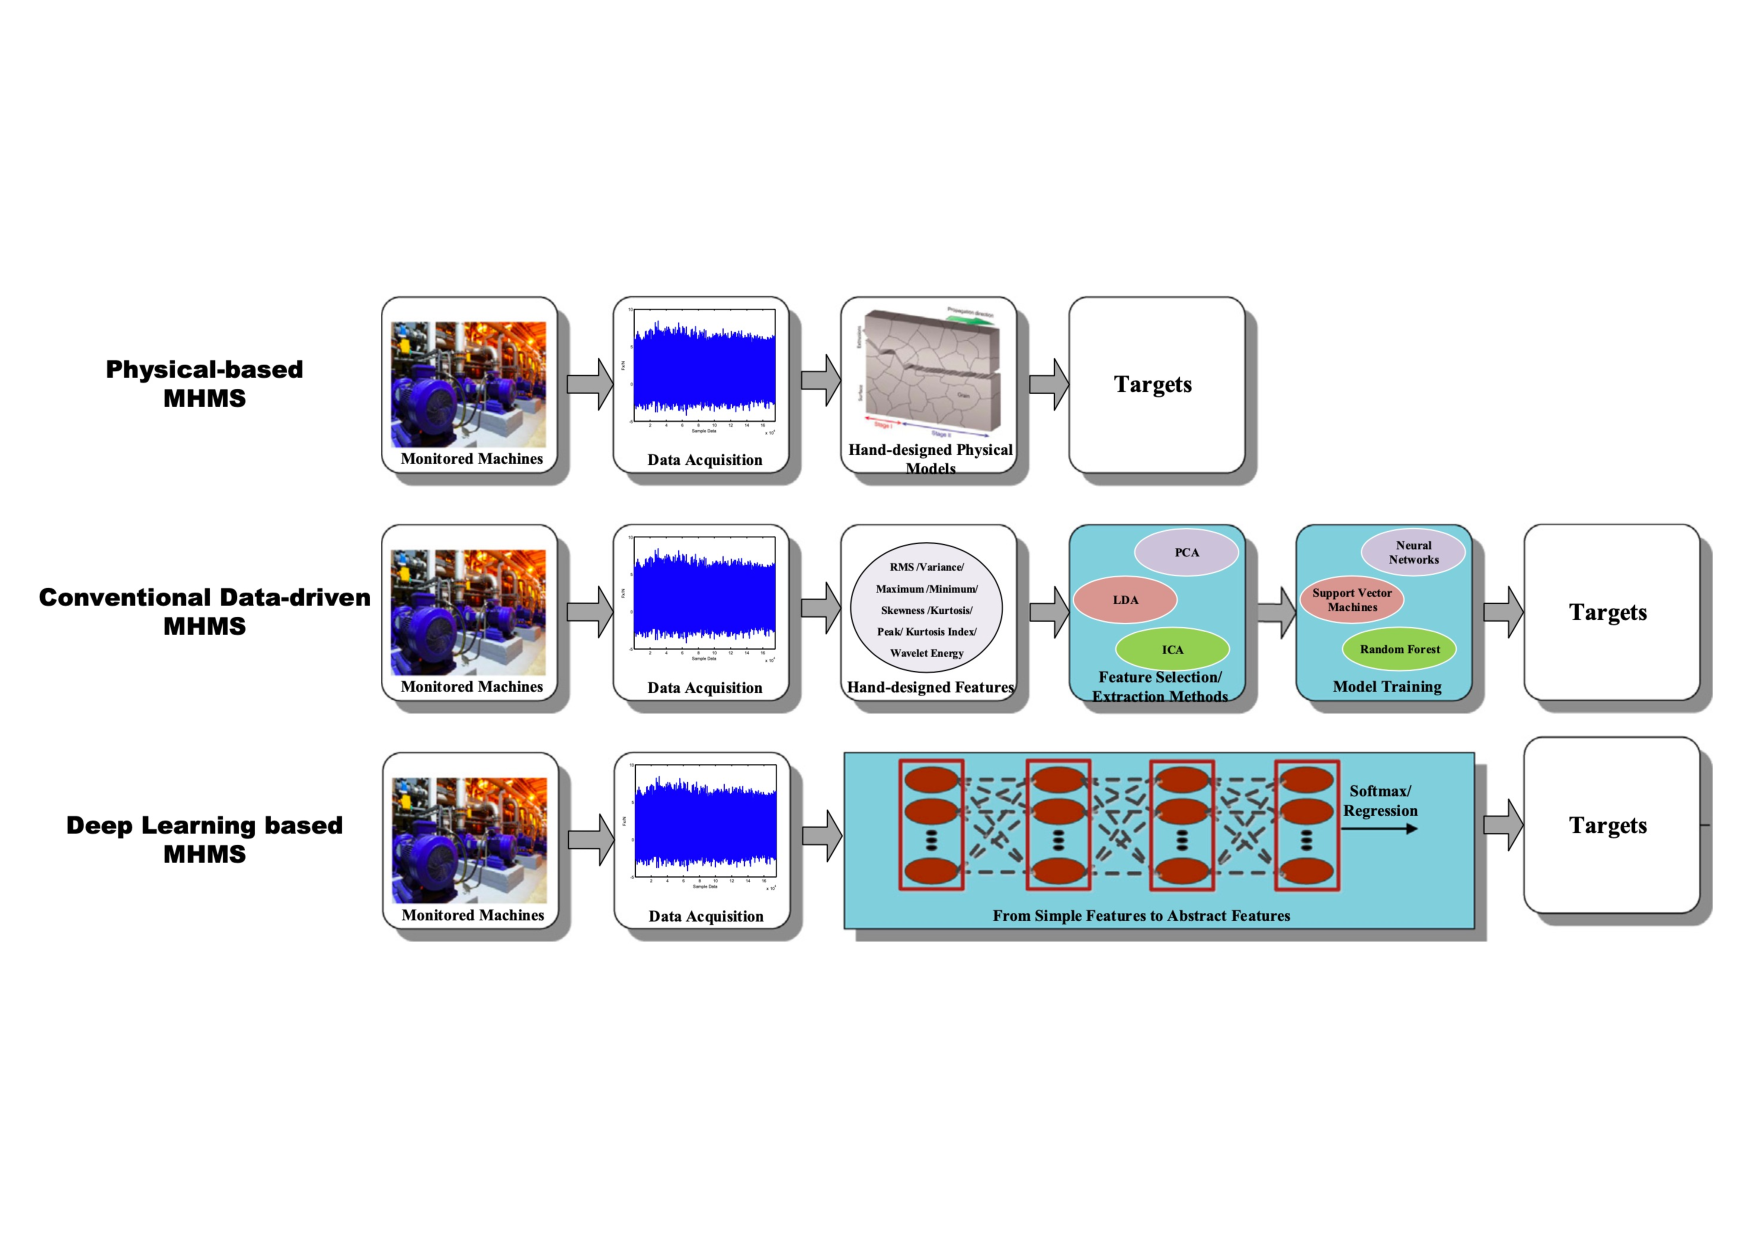
\includegraphics[width=1\textwidth]{hand_crafted_features_physical_models_deep_learning.pdf}
  \caption {Overview of different PHM approaches \cite{ZHAO2019213}} \label{fig:hand_crafted_features_physical_models_deep_learning}
\end{figure}
\chapter{Theory}\label{chapter:theory}

\section{Ball Screw Drive}
As shown in fig. \ref{fig:Ball_Screw} ball screw drives (BSDs) consist of five main components, the steel balls, screw shaft, nuts, seals, and tube. The steel balls serve as ball bearing between the screw shaft and the nuts. The screw shaft is mounted by fixed and free bearings is actuated by a motor. The nuts, which typically carry the load, move linearly along the screw shaft when the shaft is rotating. While the steel balls are rotated under external load and friction, the ball screw drive shaft is under constant compressive stress. Due to the rolling friction, defects usually occur in the grooves of the screw shaft, which guide the steel balls. Defects usually start with little abrasion on the surface of the ball screw drive shaft. Each time the steel balls pass the surface defects, the system repetitively takes shocks. Depending on the location and severity of the defects the periodicity as well as the intensity of the shock varies. For this reason, analysing recorded vibration signals seems promising for PHM systems \cite{Lee2015}. Of course surface defects also lower the efficiency of the system. Exemplary, one can imagine that the reduced efficiency leads to an increased demand of motor torque to move the load with the same speed and acceleration. This might become visible when looking at the electrical current of the motor. For this reason, also investigating the control signals of the industrial machine might be a good indicator for PHM systems. In industrial machines linear guiding shoes (LGSs) are used to guide the components that are moved by the BSDs.


\begin{figure}[H]
  \centering
  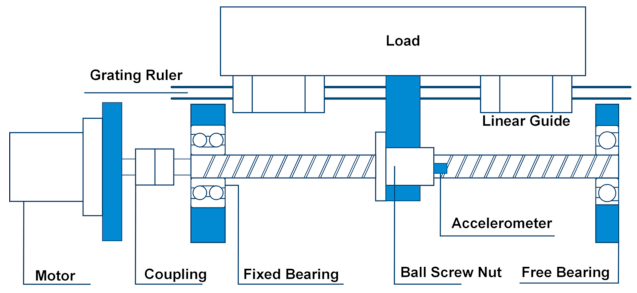
\includegraphics[width=1\textwidth]{Ball_Screw.pdf}
  \caption {Ball screw drive \cite{DENG2020}} \label{fig:Ball_Screw}
\end{figure}

\section{Neural Network}
The big data ecosystem is constantly evolving, and new technologies are coming up continuously, with many of them reacting more and more to the demands of the industry. Big data refers to an increasing volume of unstructured data, high sampling rates and a variety of different data sources. Modern technologies become relevant when processing this data to retrieve useful information. Machine learning is a research domain of algorithms that can recognize patterns in existing datasets by automatically evolving features during a training process. Deep Learning is a specific branch of machine learning. Inspired by the nature, neural networks try to imitate the function of human brains. The increased amount of data and computational power makes deep learning applications more attractive for real world use. Neural networks are hierarchically structured non-linear processing layers which try to learn hierarchical representations of data. Due to the increasing interest, the deep learning community recently came up with various new deep learning architectures. In the following, some of those are explained more in detail.

\subsection{Neural Network Architecture}
Neural networks consist of neurons which are layered in a hierarchical architecture. The neurons of consecutive layers are connected through weights and biases. During the optimization of the model, the weights and biases are updated. Fig. \ref{fig:neural_network_overview} shows the organization of neurons in an architecture with fully-connected layers. Each neuron from layer i is connected with all neurons from layer i+1 and shares information with them.

\begin{figure}[H]
  \centering
  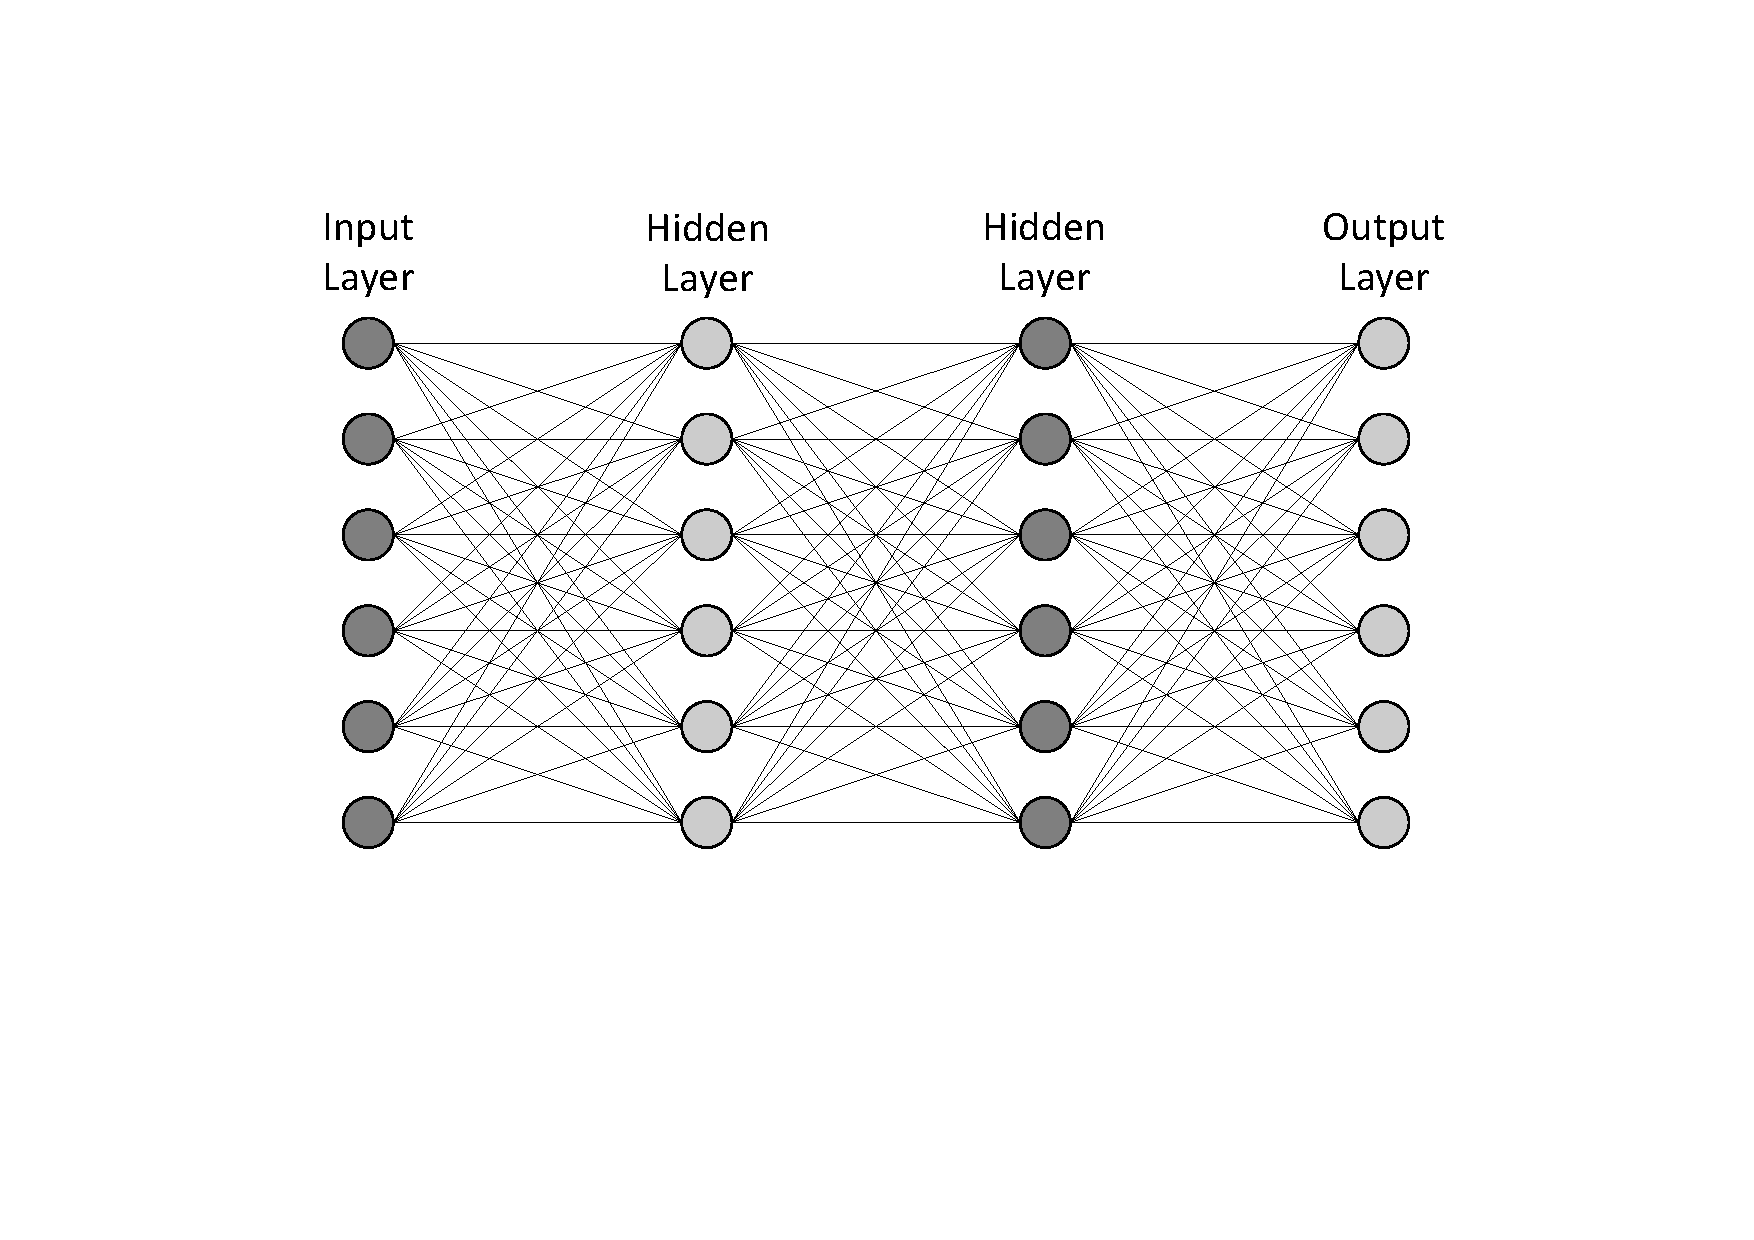
\includegraphics[width=0.7\textwidth]{neural_network_overview.pdf}
  \caption {Layer overview neural network}
  \label{fig:neural_network_overview}
\end{figure}
The input of a neuron is calculated in two steps. Firstly, the weighted sum of all previous neuron's outputs and a bias is estimated. Afterwards, the result is processed by an activation function, which gives the neural network a non-linear property. Standard multilayer feedforward networks with even one single hidden layer and an arbitrary bounded and non-constant activation function are universal approximators. This means that a wide variety of functions can be represented by the neural network when given appropriate weights \cite{HORNIK1991}. Without activation functions, neural networks could only make linear assignments of inputs x to outputs y. With rising data complexity, the demand for a "non-linear" mapping from x to y is necessary. Without a non-linearity, the set of learnable functions is identical for neural networks with several and one hidden layer. Such neural networks would not mathematically realize complex relationships in the data. Fig. \ref{fig:neural_network_optimization} shows the forward and backward pass in a neural network at the example of one single neuron. First, the outputs of the neurons $i$ from the previous layers $l-1$, which are connected with the neuron of interest $j$ in layer $l$, are multiplied with its weights and summed up together with a bias $b_{j}$. The resulting logits $z_{j}$ are then processed by the activation function $\phi$. Different activation functions can be used throughout the network. After passing several consecutive hidden layers, a loss function evaluates the prediction with the ground truth label in the end of the network.

\subsection{Activation Function}
Different problems and network layers require different activation functions. One typically uses tanh, sigmoid and ReLU activations in hidden layers and a linear, sigmoid and softmax function in the final layer \cite{Brownlee2021}. Linear final layers are restricted to regression problems, whereas sigmoid and softmax functions are used for classification problems. The sigmoid function is used for binary and softmax for multiclass classification. In general, the softmax function is an extension of the sigmoid function to the multiclass case, which can be proofed easily. The softmax and sigmoid functions normalize the network output to a probability distribution over the predicted output classes. Deciding for activation functions in the hidden layers does not follow such clear rules. All the mentioned functions have different characteristics, which lead to individual advantages and disadvantages. The sigmoid and tanh activation function squeeze the inputs in values between -1 and 1. Both functions can suffer from the vanishing gradient problem, since the derivative of these functions is close to zero for very big or small inputs. A solution for that is the ReLU activation function, which solves that problem but maps all negative inputs to zero. This so-called dead ReLU problem is solved by the Leaky Relu functions.  \cite{Brownlee2021}. In table \ref{tab:activation_functions} some of the most popular activation functions are described.

\begin {table}[H]
\begin{tabular}{ c c c c }
\toprule 
Formula & Formulation s(x) & Derivative $\frac{ds(x)}{dx}$ & Function Output Range \\
\midrule 
ReLU &   $\begin{cases} 0 & \text{, for }x < 0\\
	x & \text{, for }x \geqslant 0 \end{cases}$ & $\begin{cases} 0 & \text{, for }1 < 0\\
	1 & \text{, for }x \geqslant 0 \end{cases}$ & $[ 0, \infty)$\\

\rule{0pt}{5ex}%  EXTRA vertical height 

Leaky ReLU &   $\begin{cases} \alpha x & \text{, for }x < 0\\
	x & \text{, for }x \geqslant 0 \end{cases}$ & $\begin{cases} \alpha & \text{, for }1 < 0\\
	1 & \text{, for }x \geqslant 0 \end{cases}$ & $(- \infty, \infty)$\\

\rule{0pt}{5ex}%  EXTRA vertical height 

Sigmoid & $\frac{1}{1+e^{-x}}$ & $\frac{e^{-x}}{(1+e^{-x})^{2}}$ & (0,1)\\

\rule{0pt}{5ex}%  EXTRA vertical height 

Softmax & $\frac{e^{x_{i}}}{\sum_{j=1}^{K} e^{x_{j}}}$ & $\frac{e^{-x}}{(1+e^{-x})^{2}}$ & (0,1)\\

\rule{0pt}{5ex}%  EXTRA vertical height 

tanh & $\frac{e^{2x}-1}{e^{2x}+1}$ & $1-tanh^{2}(x)$ & $(-1,1)$ \\
\bottomrule  

\end{tabular}
\caption {Overview activation functions} \label{tab:activation_functions}
\end {table}
\subsection{Optimization}
When training neural networks one has to decide for a loss function and an optimizer. 

\subsubsection{Loss}
The loss function acts as a model evaluation criterion and the optimizer is responsible for changing the model according to the criterion. Deep learning can be applied in two different use cases: (1) regression tasks and (2) classification tasks. In a regression problem, the goal is to learn a mapping function from input variables to a continuous output variable. Contrariwise, in a classification problem, the model aims to predict a class label for each input sample \cite{ShilohPerl2020}. Typically, the mean square error (MSE) is applied as criterion in regression tasks:

\begin{equation}
L(X) =  \sum_{x}(\hat{y}(x)-y(x))^2,
\end{equation}

where $y(x)$ is the ground truth and $\hat{y}(x)$ the predicted class label \cite{ShilohPerl2020}. On the other hand, a Cross-Entropy-loss (CE-loss) is common for classification tasks: 

\begin{equation}
L(X) = \sum_{x} y(x) log(p(x)),
\end{equation}
where p(x) is the predicted probability of the sample $x$ belonging to the ground truth class $y(x)$ \cite{ShilohPerl2020}.

\subsection{Training Loop}
During training, the model's weights and biases need to be adapted such that the criterion is minimized. This optimization takes place in a two stage process:
\begin{itemize}
    \item \textbf{Forward pass}: Calculating the neuron values throughout the network and the loss from the model prediction and the ground truth values or classes.
    \item \textbf{Backward pass}: Calculating the derivative of the criterion with respect to the model parameter and updating those to reduce the loss.
\end{itemize}
Iteratively, these two steps are performed to optimize the model. The process is visualized in fig. \ref{fig:neural_network_optimization}. By calculating the partial derivatives of each layer and concatenating them in a reverse order of the forward pass, the gradients used for updating the model parameters can be established. For concatenating the partial derivatives, the chain rule is used:
\begin{equation}
 \frac{\delta L_{i}}{\delta w_{i}} = \frac{\delta L_{i}}{\delta \hat{y_{i}}} \cdot \frac{\delta \hat{y_{i}}}{\delta z_{i}} \cdot \frac{\delta z_{i}}{\delta w_{i}}, 
 \label{chain_rule}
\end{equation}
where $\frac{\delta L_{i}}{\delta \hat{y_{i}}}$ is the derivative of the loss with respect to the activation in the final layer, $\frac{\delta \hat{y_{i}}}{\delta z_{i}}$ is the derivative of the used activation function.  $\frac{\delta z_{i}}{\delta w_{i}}$ is the derivative of the logits $z_{i}$ with respect to the weights and biases used between the last two layers of the network \cite{ShilohPerl2020}. The gradients for all the previous layers needs to be estimated and concatenated equally to update all parameters in the model.

\begin{figure}[H]
  \centering
  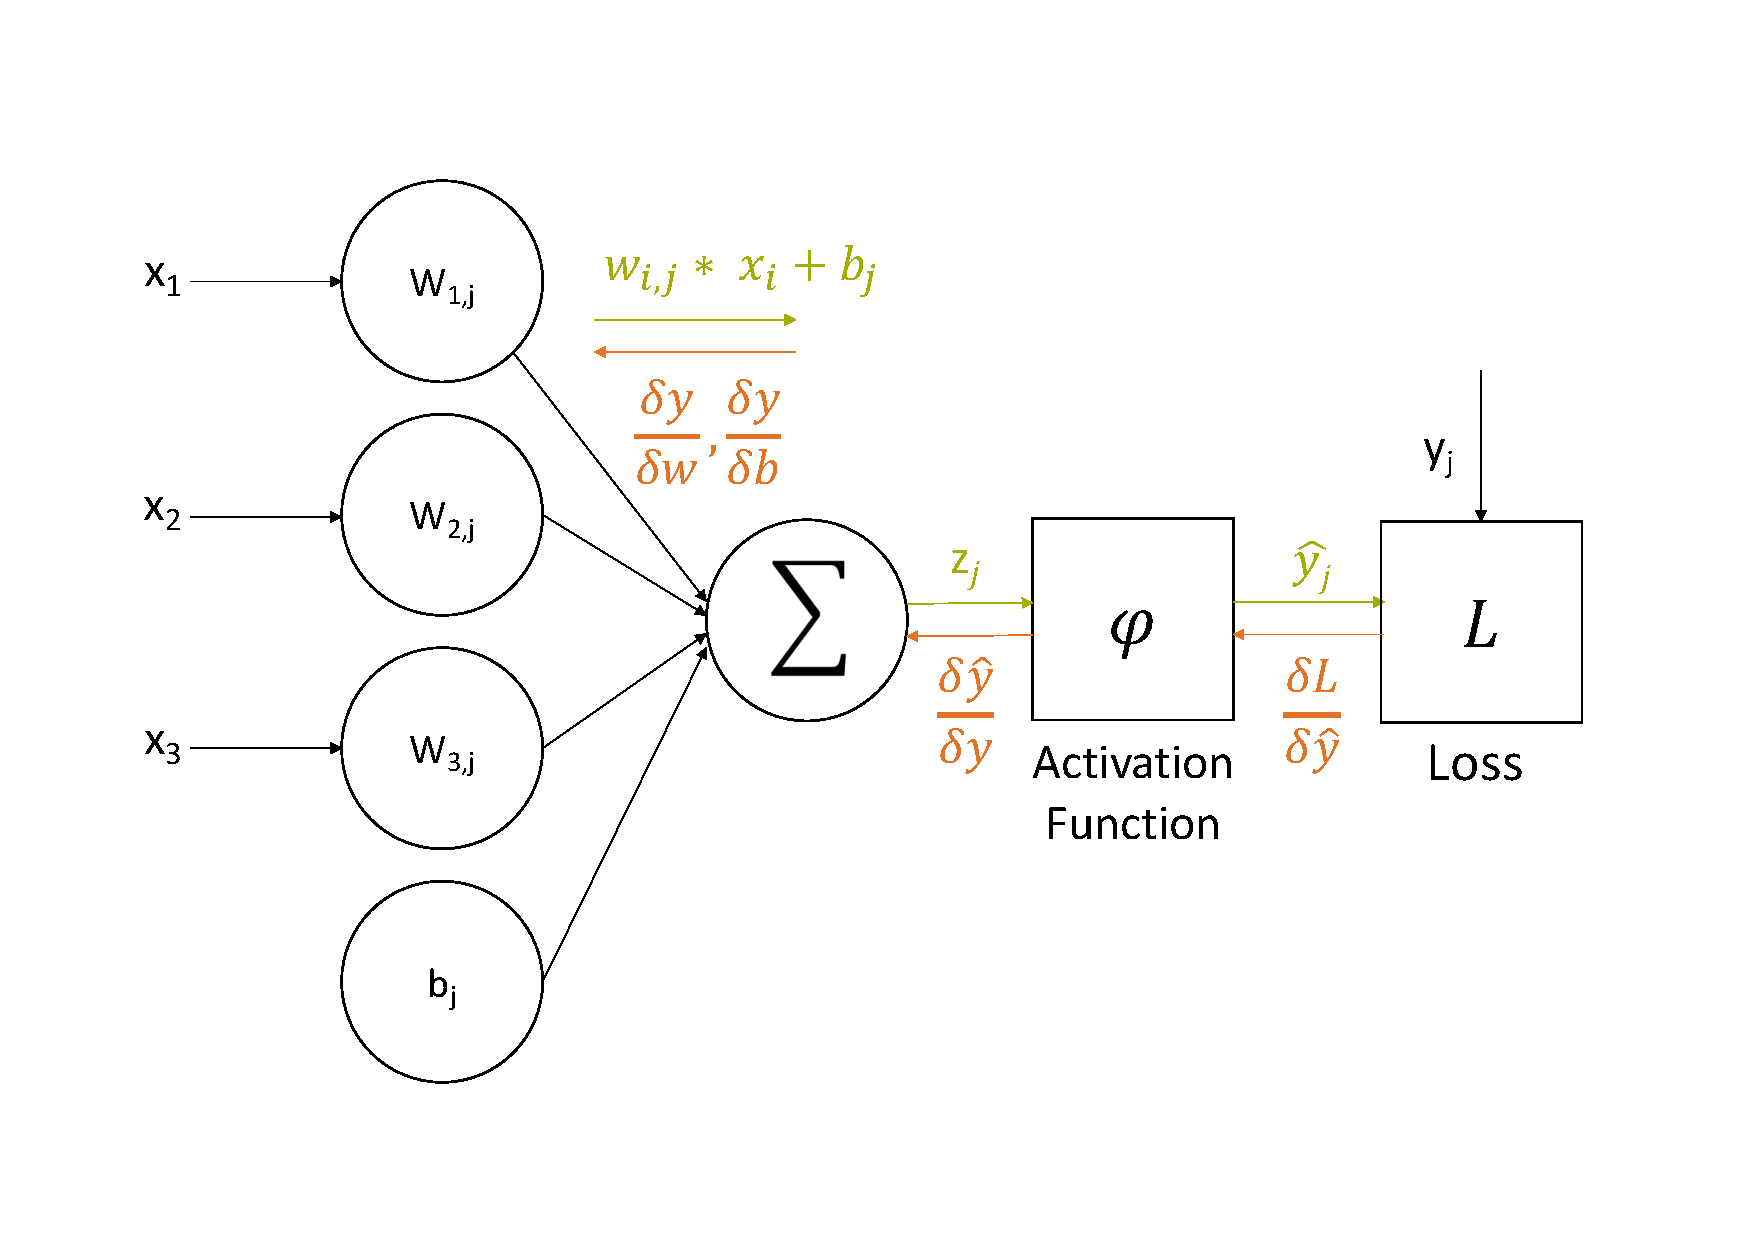
\includegraphics[width=0.7\textwidth]{neural_network_optimization.pdf}
  \caption {Optimization of neural network}
  \label{fig:neural_network_optimization}
\end{figure}

\subsection{Optimizer}
Calculating the gradient for the whole dataset is computationally expensive. A common practice is therefore to separate the dataset in several subsets, so called mini-batches. For each mini-batch, the gradients are calculated and the model is updated. This process is repeated for all the mini-batches retrieved from the dataset. Each training loop including the whole dataset is called an epoch. As soon as the loss converges the training can be terminated. Despite convergence, an optimal solution is not assured since the most neural network problems are not convex \cite{ShilohPerl2020}.

Most optimization methods are first order methods, which rely on gradients to update the model parameters. Second-order methods combine second and first order derivatives, which generally makes the method converge faster. These methods require the computation of the Hessian, which is especially expansive for big datasets and models. Also, first order methods can suffer from long training times when calculating gradients for big datasets (batch gradient descent). A method which tries to circumnavigate this problem is the Stochastic Gradient Descent (SGD). Repetitively, the model is updated with gradients based on a single sample, which is picked randomly from the dataset. Since the choice of these samples is random, the optimization suffers from instability and fluctuation. The mini-batch gradient descent is a compromise between the regular SGD and batch gradient descent. The gradient and model update is neither performed for a single sample nor for the whole dataset. It is performed on a small and randomly picked subset of the data, which accelerates the convergence of the training.
In order to accelerate and stabilize the optimization, one can also include historical gradients and update the model weights with a moving average over the past gradients. First and second order momenta are methods which accelerate SGD in the relevant direction and dampens oscillations \cite{ShilohPerl2020}. This variant of the regular gradient descent allows an optimization with an adaptive step size in the different dimensions of the latent feature space. To learn faster, the step size can be increased in the relevant and decreased in the irrelevant directions. Each training loop including the whole dataset is called an epoch. As soon as the loss converges, the training can be terminated. Despite convergence an optimal solution is not assured since the most neural network problems are not convex \cite{ShilohPerl2020}.\newline\newline

\textbf{Momentum}
Updating the model parameters with momentum is a procedure which includes two steps. In a first step, the moving average over the past gradients is calculated and in a second step the model parameters are updated accordingly:

\begin{equation}
  \begin{aligned}
      v_{t} = & \gamma v_{t-1} +  \eta \nabla_{\theta}L(W_{t-1}) &\\
      W_{t} = &W_{t-1} - v_{t},
      \label{eqn:momentum}
  \end{aligned}
\end{equation}

where $v_{t}$ is the updated and $v_{t-1}$ the current momentum, $W_{t}$ is the updated and $W_{t-1}$ the current model weights, $\nabla_{\theta}L(W_{t-1})$ is the derivative of the loss with respect to the current model weights, $\eta$ is the learning rate and $\gamma$ defines the relationship between the current momentum and gradient for calculating the updated momentum \cite{Ruder2016}.
\newline
\newline
\textbf{Nesterov Accelerated Gradient}
\newline
Another well known optimizer of this kind is Nesterov Accelerated Gradient (NAG), which extends the regular first order momentum update rules. When calculating the first order momentum, NAG calculates the gradient not with respect to the current but to the pre-updated weights: 

\begin{equation}
    \nabla_{\theta}L( W_{t-1} - \gamma v_{t-1}),
\end{equation}

where $W_{t-1}$ are the current model weights, which are pre-updated with the current first order momentum $v_{t-1}$. Just like described in equation \ref{eqn:momentum} the pre-updated gradient is used to calculate the updated momentum in a first step, which is then applied to update the model weights in a second step \cite{Ruder2016}.
\newline
\newline
\textbf{Adagrad}
\newline
Like all mentioned optimization methods also Adagrad is a gradient-based optimization. Adagrad uses a squared version of the moving average over the past gradients:

\begin{equation}
  \begin{aligned}
  W_{t} = W_{t-1} - \frac{\eta}{\sqrt[2]{G_{t}+ \epsilon}} \bigodot \nabla_{\theta}L(W_{t-1}),
  \end{aligned}
  \label{eq:Adagrad}
\end{equation}

where  $W_{t-1}$ are the current and $W_{t}$ the updated model weights, $\nabla_{\theta}L(W_{t})$ is the derivative of the loss with respect to the current model weights. $G_{t}$ is the second order momentum, which is a diagonal matrix where each diagonal element i,i is the sum of the squares of the gradients with respect to the model parameter i up to time step t. $\epsilon$ denotes a small quantity which prevents the division by zero and $\gamma$ is the learning rate \cite{Ruder2016}.
\newline
\newline
\textbf{Adaptive Moment Estimation}
\newline
Adaptive Moment Estimation (Adam) is one of the most popular optimizer. ADAM combines the idea of first and second order momentum: 
\begin{equation}
  \begin{aligned}
   &m_{t} =  \beta_{1} m_{t-1} +  (1-\beta_{1}) \nabla_{\theta}L(W_{t-1}) &\\
    &v_{t} =  \beta_{2} v_{t-1} +  (1-\beta_{2}) \nabla_{\theta}L^{2}(W_{t-1}) &\\
    &\hat{m}_{t} = \frac{m_{t}}{1-\beta_{1}^{t}}&\\
    &\hat{v}_{t} = \frac{v_{t}}{1-\beta_{2}^{t}}&\\
   & W_{t} = W_{t-1} - \frac{\eta}{\sqrt[2]{\hat{v}_{t} + \epsilon}}\hat{m}_{t}, &\\
  \end{aligned}
  \label{eq:ADAM}
\end{equation}

where $m_{t}$ and $v_{t}$ are the first and second momentum, $\hat{m}_{t}$ and $\hat{v}_{t}$ are the bias-corrected first and second moment estimates, $\beta_{1}$ and $\beta_{2}$ are the weighting factors for the moving average and $W_{t-1}$ and  $W_{t}$ are the current and updated model weights \cite{Ruder2016}.

\section{Convolutional Neural Network}

Equally, to regular neural networks, convolutional neural networks (CNNs) consist of several neurons embedded in a fixed architecture. Developed for computer vision applications, the architecture of CNNs is optimized to process images. In CNNs the neurons are structured in layers just like in normal neural networks. In regular networks the neurons of one layer are organized in one dimension and in CNNs in three dimensions (height, width, depth). The functionality of CNNs is visualized in \ref{fig:CNN_overview}. One can identify four main compounds of a CNN, which are described more detailed in the following:

\begin{itemize}
    \item [1.] The input data is organized in a structured and grid-like form. Each element in this structure is called a pixel, which described by its specific value and position. The data is stored in arrays with spatial dimension (height x width) and depth (channel size).
    
    \item [2.] Convolutional layers contain kernels which are convolved with the input. The kernel contains weights and biases which are learned during training. An 'elementwise' activation function is applied to the kernel outputs.
    
    \item [3.]  Pooling layers downsample the spatial dimension. This reduces the height and width of the feature maps throughout the network. This minimizes the learnable network parameters.
    
    \item [4.] In the end fully-connected layers coupled with activation functions attempt to predict class labels for the input data.
\end{itemize}

\begin{figure}[H]
  \centering
  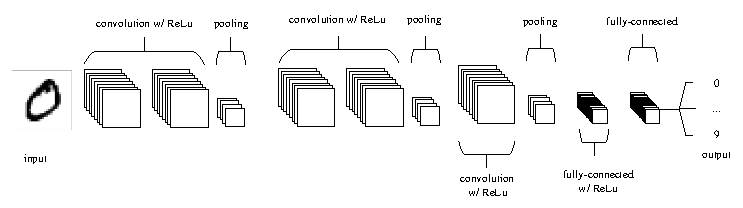
\includegraphics[width=0.9\textwidth]{cnn/cnn_architecture.pdf}
  \caption {CNN architecture \cite{OShea2015}}
  \label{fig:CNN_overview}
\end{figure}

In the following typical CNN layers are described more in detail. 

\subsection{Kernel}
The convolutional layers are the core elements in a CNN. The learnable parameters in a convolutional layer are the weights and biases of the kernel. During the optimization, each kernel learns to extract expressive features. The depth of a kernel is defined by the depth of the input layer and the number of applied kernels defines the depth of the subsequent feature map. Each channel corresponds to the features extracted by the convolution of a single kernel with the data across the whole spatial dimension. Usually, the spatial dimensions (width, height) are reduced and the depth of the latent feature map is increased throughout the network. Therefore, the network extracts more global features in the beginning and more local features in the end of the network.  \cite{OShea2015}. Looking at fig. \ref{fig:kernel_number} one can see how the kernel of depth 3 is applied to the input of depth 3. By using 6 kernels, the resulting feature map is of depth 6.

\begin{figure}[H]
  \centering
  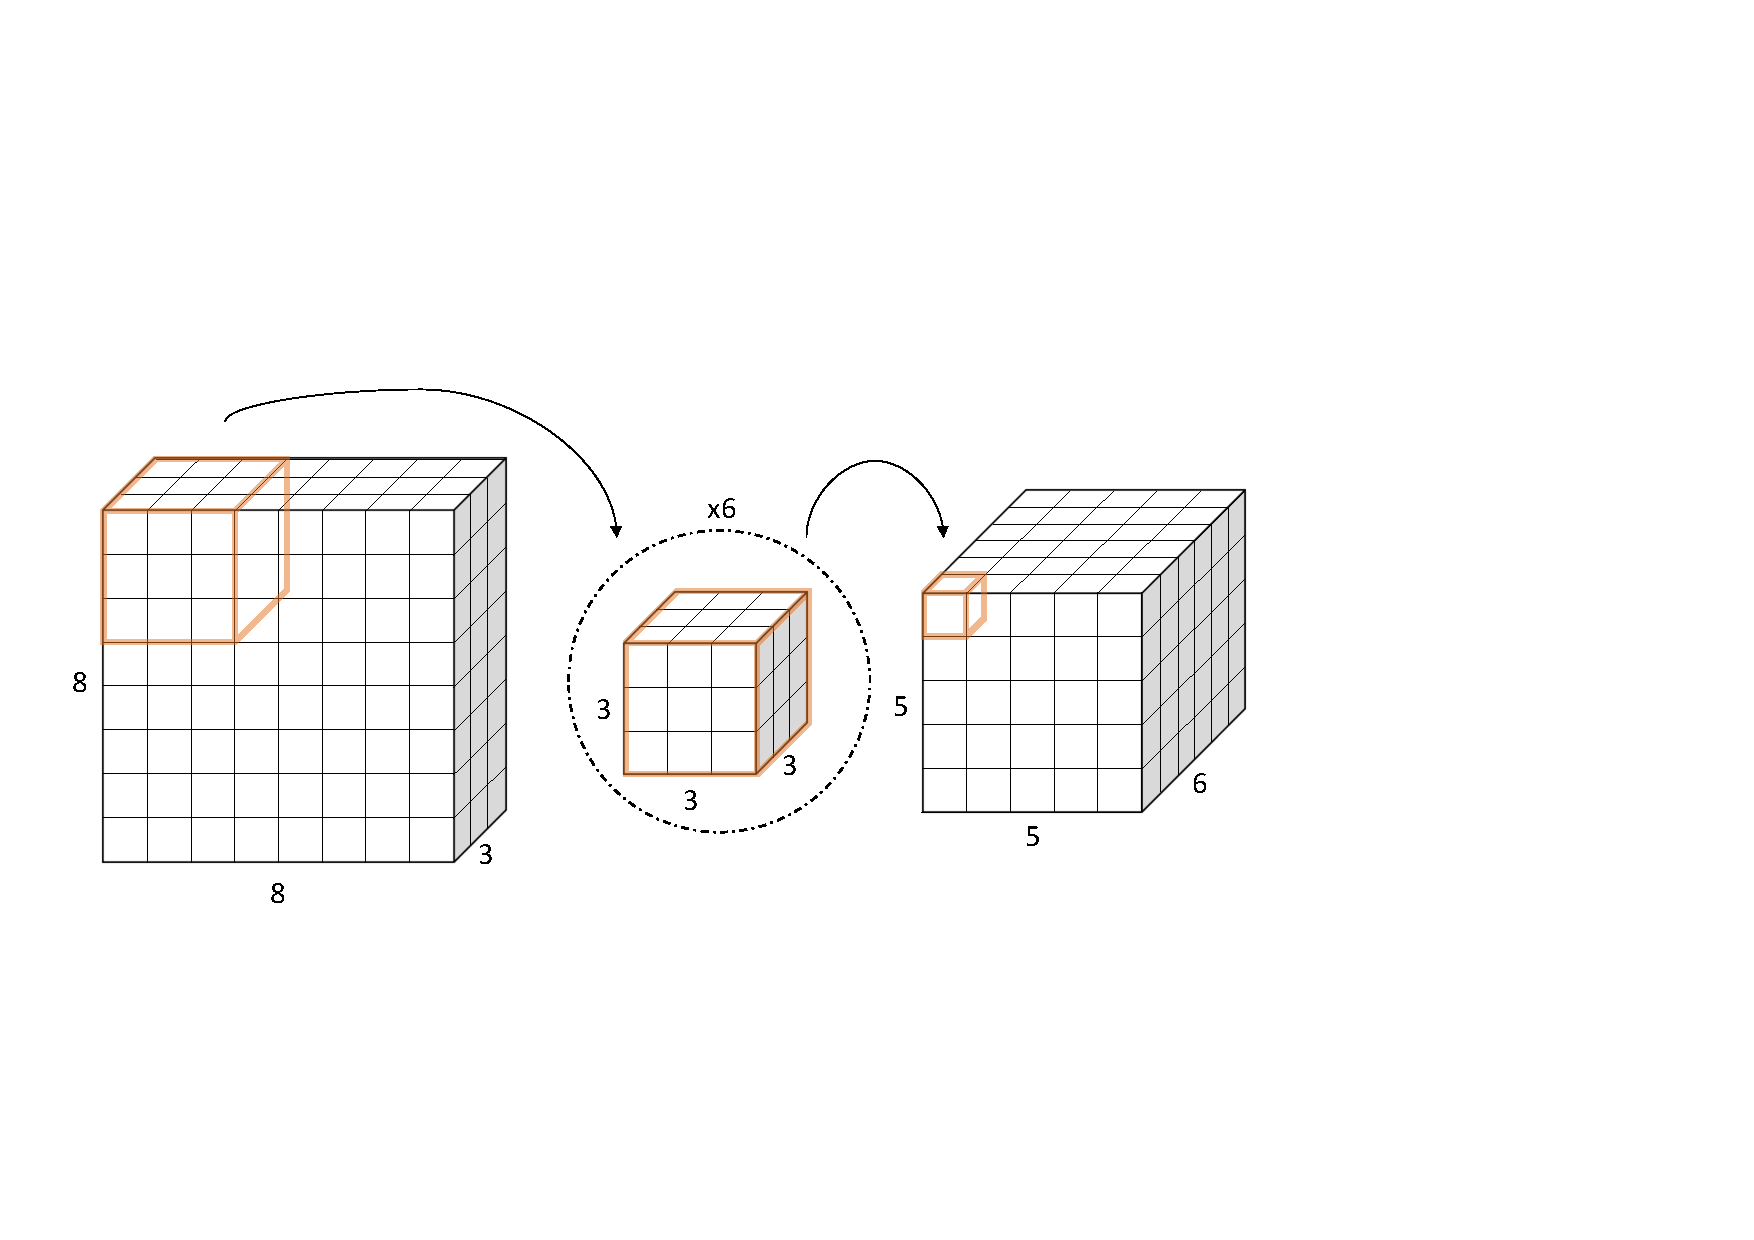
\includegraphics[width=0.6\textwidth]{cnn/kernel_number.pdf}
  \caption {2D convolution based on \cite{Ganesh2019}}
  \label{fig:kernel_number}
\end{figure}

To make things easier a single convolution of a kernel with a subspace of the input data is shown for the 1D case:

\begin{equation}
  y(p_{0}) = \sum_{p_{n} \in R} w(p_{n}) \cdot x(p_{0} + p_{n}), 
  \label{eq:kernel}
\end{equation}

where $p_{n}$ is one of the $R$ kernel cells, $p_{0}$ is the lower bound pixel position of the input subspace involved in the single convolutional operation. Each kernel cell is multiplied with a corresponding pixel in the input and the $R$ outputs are summed up in the pixel $p_{0}$ of the subsequent feature map \cite{Ganesh2019}. Typically, a bias value is included in this weighted sum and a non-linearity is applied consecutively. The convolutional process is also visualized in fig. \ref{fig:kernel}, where $p_{n}$ is one of the three cells within the kernel, $R$ is three in this case and $p_{1}$ marks the lower bound pixel position of the input feature map and the pixel which sums all the information from the convolution in the output feature map.


\begin{figure}[H]
  \centering
  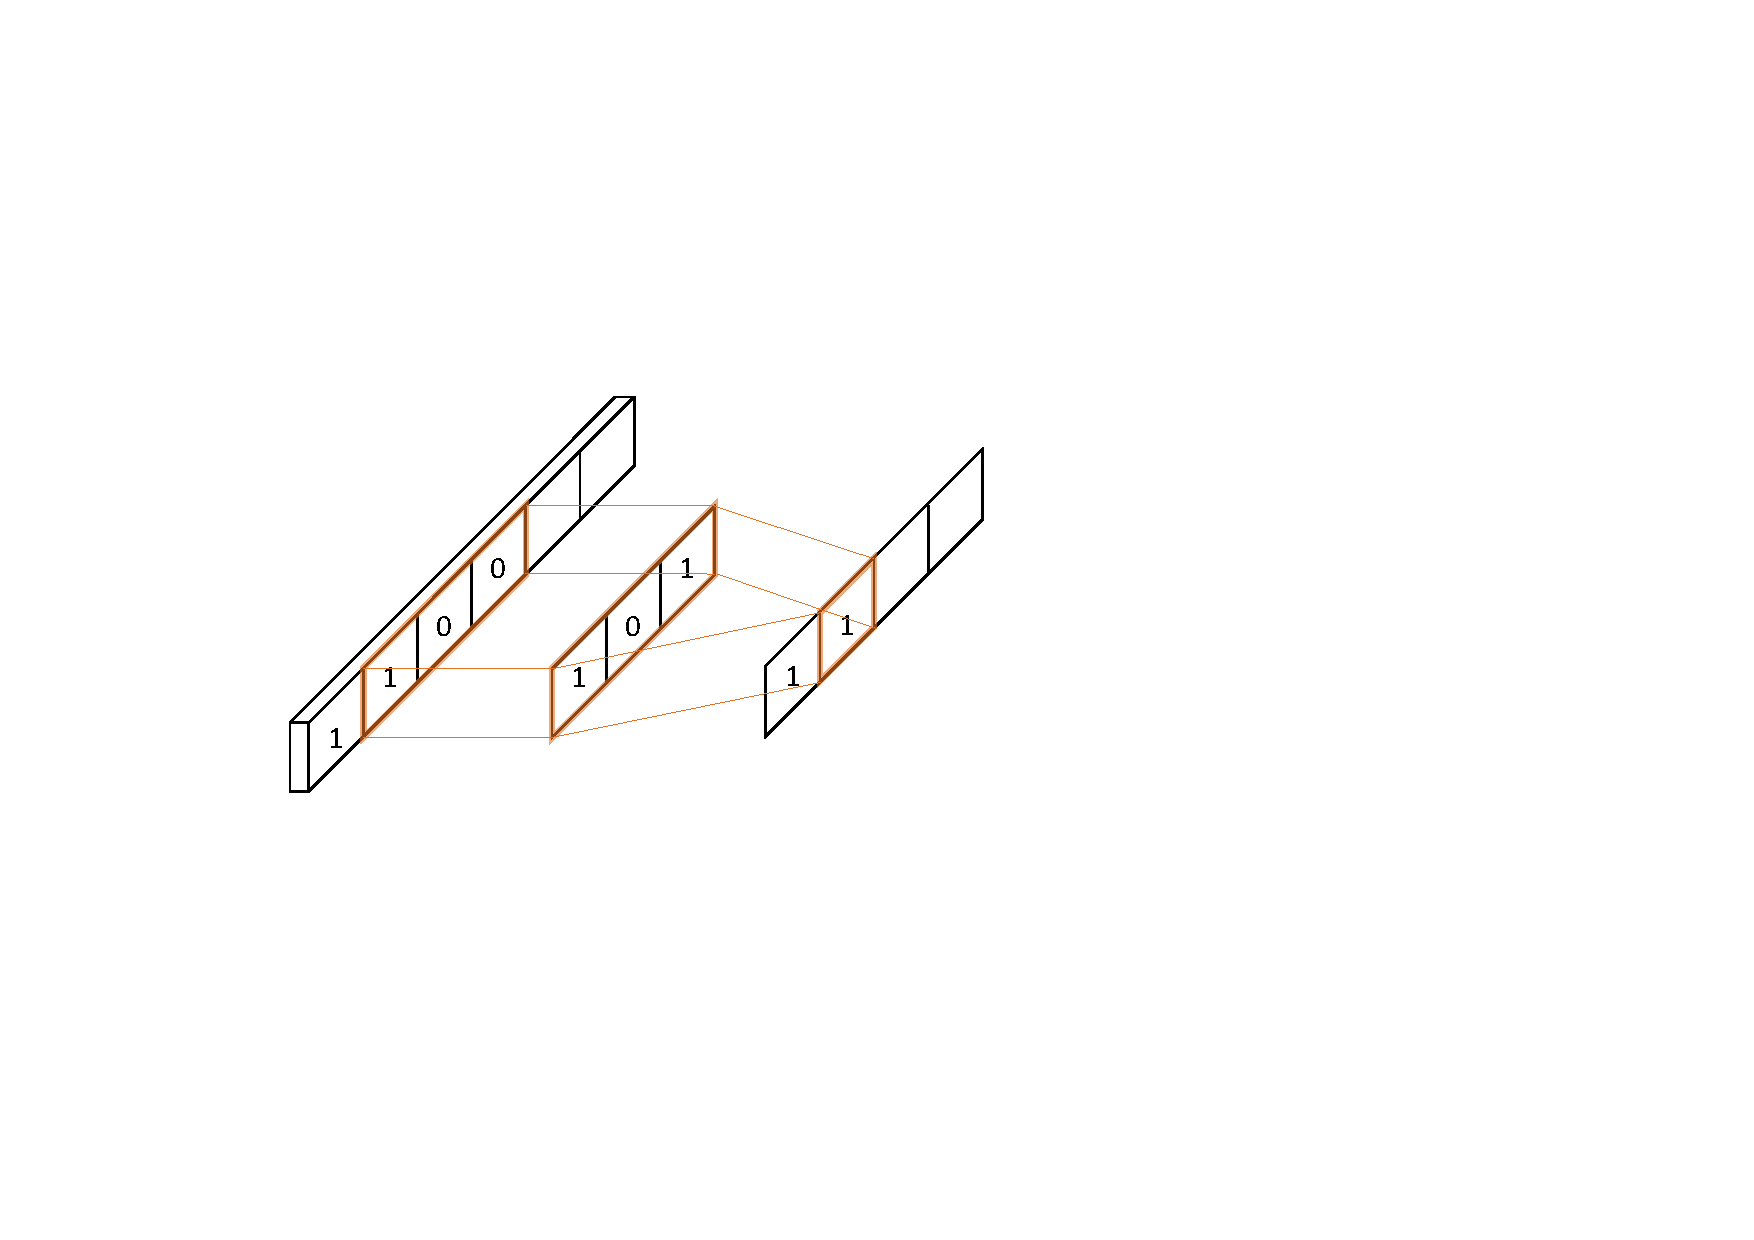
\includegraphics[width=0.4\textwidth]{cnn/kernel_calculation.pdf}
  \caption {1D convolution based on \cite{Ganesh2019}}
  \label{fig:kernel}
\end{figure}

Compared to regular neural networks CNNs profit a lot from its weight sharing concept. The kernel weights are learned throughout the training. Since the same kernel is applied on different areas of the input, it is not necessary to train a weight for every pixel along the whole spatial dimension of the input. This reduces the number of learnable parameters in the network \cite{OShea2015}. Since the kernel is applied on different areas of locations, the feature search is insensitive to feature location in the image.

\subsection{Convolution Parameters}

The dimension of the input, which is processed by the kernel, is called receptive field. When increasing the receptive field, more global and otherwise more local features of the input are extracted. When defining a CNN architecture, one has to find a trade-off between a model which is complex enough to capture important information from the data and also keep the number of parameters low. Several hyperparameters can be used to reduce or increase the complexity of the model. After a convolutional layer, three hyperparameters can be used to define the width and height of the resulting feature map. 


\subsection{Stride}
By increasing the stride, the kernel skips several input pixels while shifting the kernel. The effects of different stride factors are shown in fig.\ref{fig:stride_cnn}. Also, this convolution variant decreases the spatial dimension of the resulting feature map \cite{OShea2015}.

\begin{figure}[H]
  \centering
  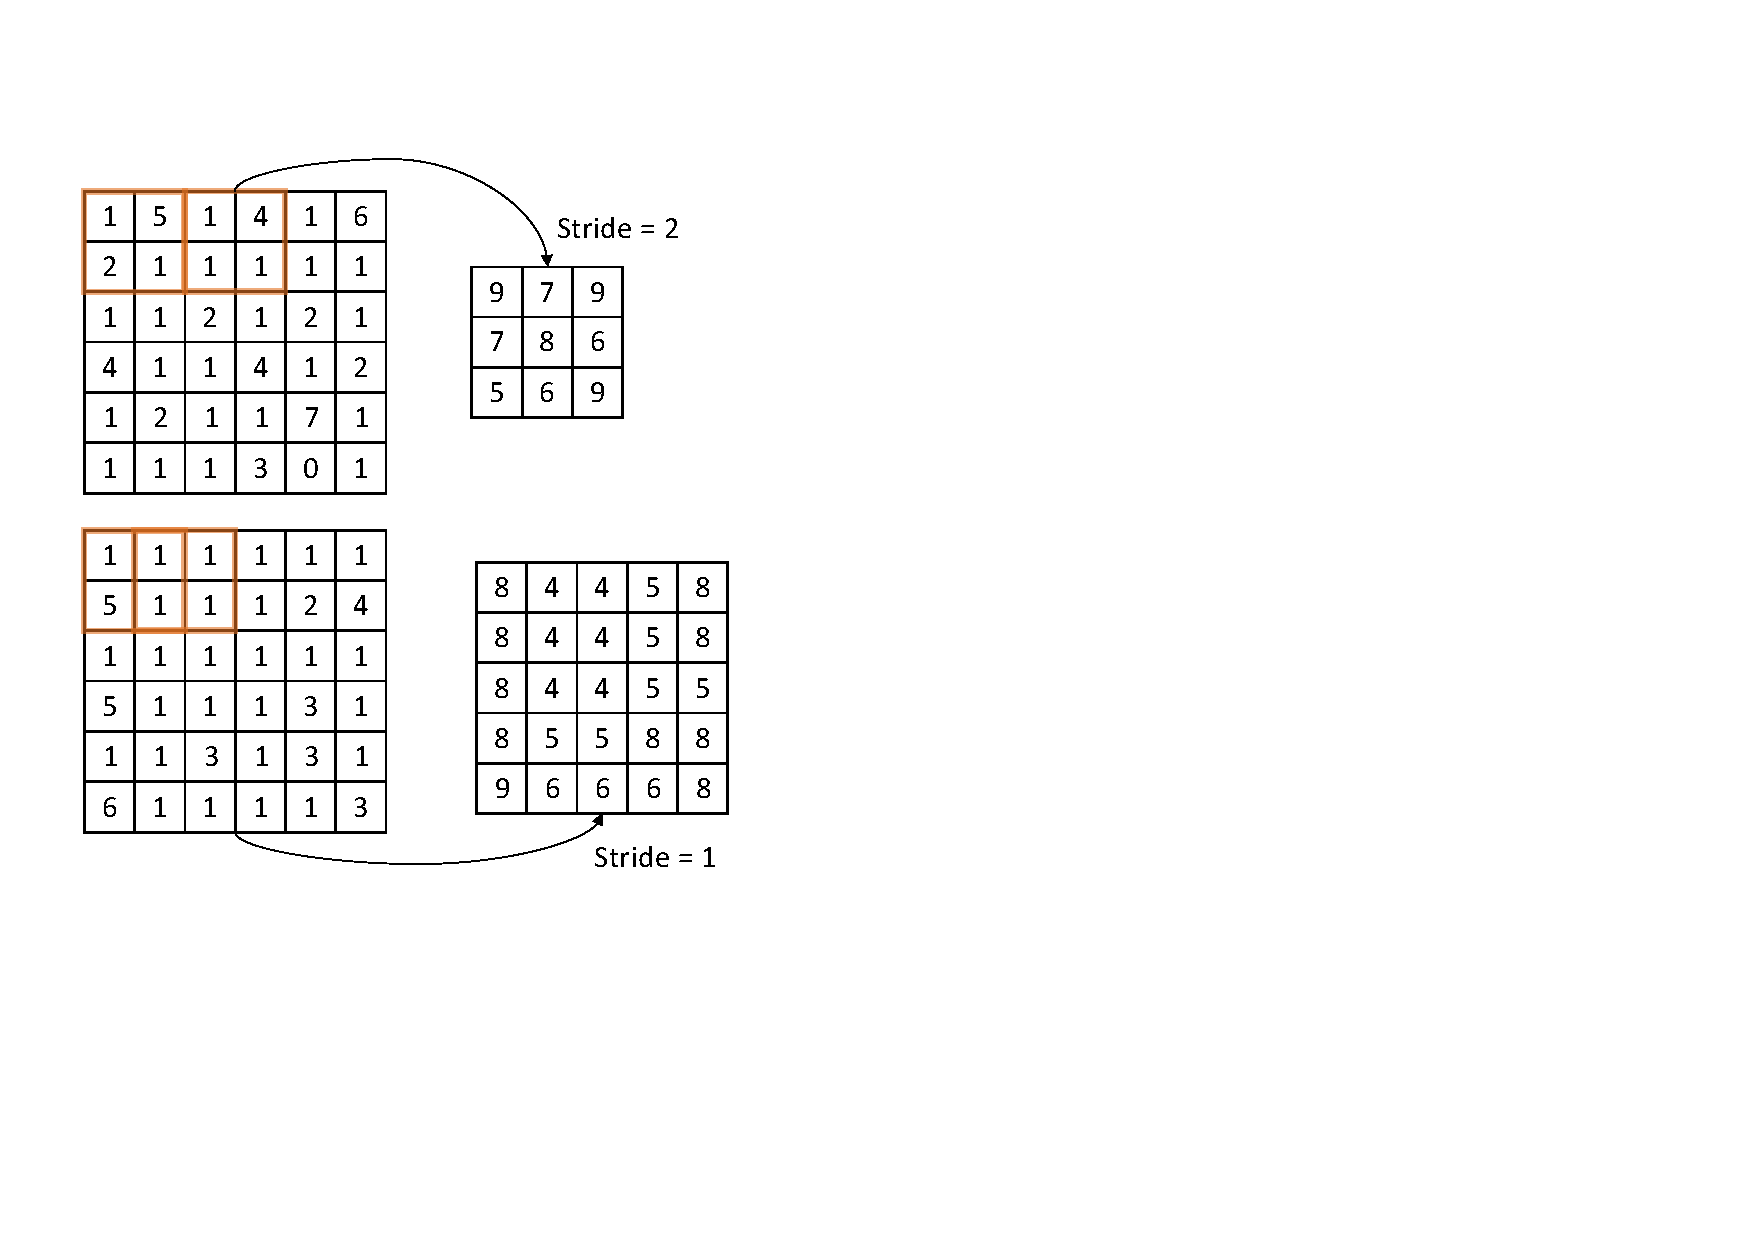
\includegraphics[width=0.4\textwidth]{cnn/stride_cnn.pdf}
  \caption {Stride factor}
  \label{fig:stride_cnn}
\end{figure}


\subsection{Zero Padding}
Zero padding, shown in fig.\ref{fig:zero_padding_cnn}, enlarges the input with a border of zeros. During the convolution, the kernel covers an increased spatial dimension of the input, which increases the spatial dimension of the resulting feature map \cite{OShea2015}.

\begin{figure}[H]
  \centering
  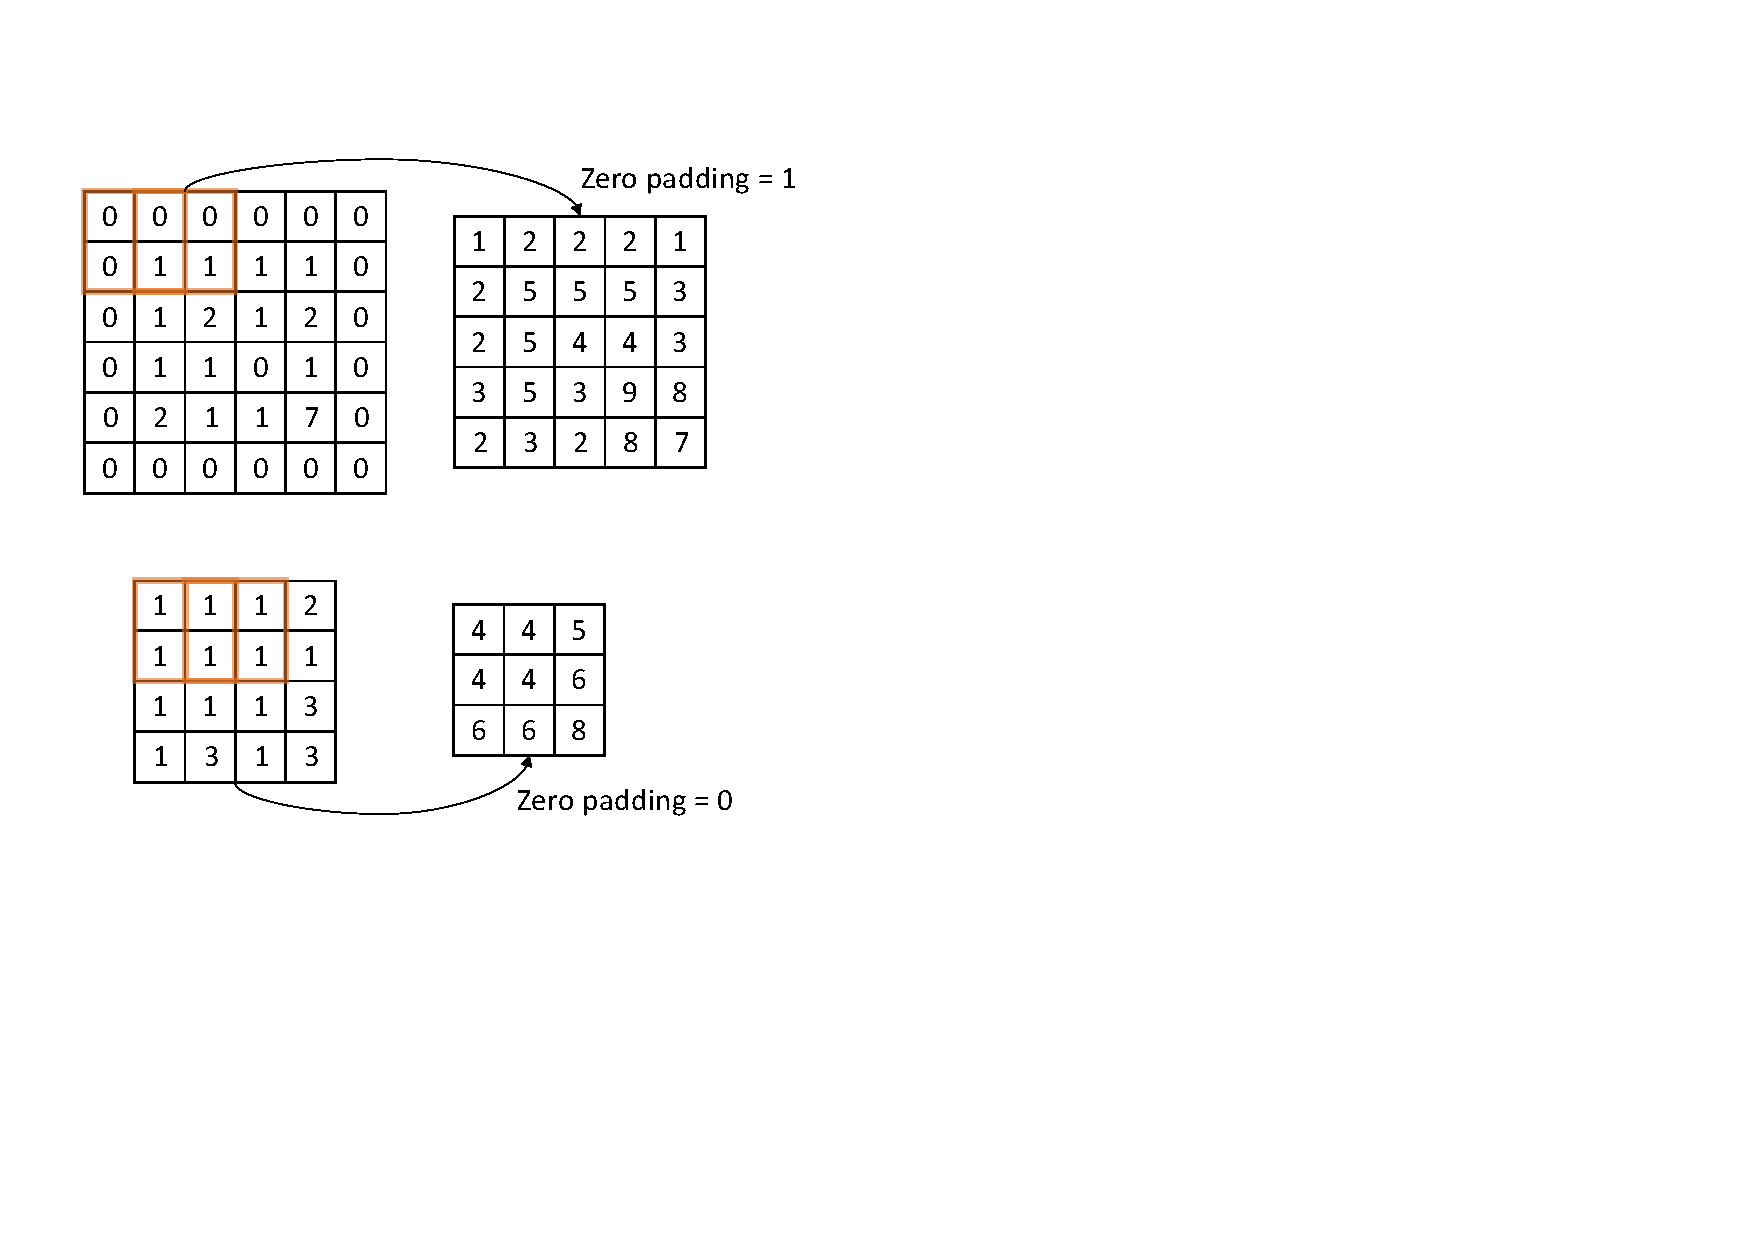
\includegraphics[width=0.4\textwidth]{cnn/zero_padding_cnn.pdf}
  \caption {Zero padding}
  \label{fig:zero_padding_cnn}
\end{figure}



\subsection{Spatial Dimension}

 The spatial dimension of the feature map right after a convolutional layer can be calculated as follows:

\begin{equation}
  \frac{(V-R)+2Z}{S+1}, 
  \label{eq:spatial_dimensionality_cnn_feature map}
\end{equation}
where V is the input size, R is the size of the receptive field, Z is the amount of zero padding and S refers to the stride.

\subsection{Pooling Layer}
To change the spatial dimension of the latent feature spaces throughout the network, one can also include pooling layers. There exist different variants like max- and average-pooling. In general, the functionality is similar to convolutional layers with the only difference that no learnable parameters are involved. Also pooling kernels are shifted over the input. For each kernel position, all pixels covered by the kernel are merged to a single value. Max-pooling returns the maximal pixel value and average-pooling the average over all pixels. Often convolutional and pooling layers are applied consecutively \cite{OShea2015}.


\section{Domain Adaptation and Transfer Learning}

In the computer vision community, domain adaption and transfer-learning techniques recently received more and more attention. Transfer learning, also called multi-task learning, is a problem related to domain adaption. The goal is to train a model to solve a specific task on a given dataset. The model should then be used to solve a different task on the same data. The data used in the tasks is equally distributed, but in different tasks the relation between samples and ground truth outputs differs. For this reason, the conditional distribution differs, whereas the marginal distribution is the same for the different tasks. Domain adaption refers to problems in which a model is trained on labeled train data, denoted as source domain. The model is then applied to solve an equal task on the unlabeled test data, denoted as target domain. The target and source domain data come from different distributions, anyhow the data must be related in any sense and structured similarly. The conditional and marginal distribution for the source and target domain data differ. Generally, one can say domain adaption is used to reduce the discrepancy between data distributions. In this sense, a model is trained to solve the same task on differently distributed data. Transfer learning on the other hand learns a model, which is able to solve different tasks on the same dataset. The differences are visualized in fig. \ref{fig:domain_adaption_vs_transfer_learning}

\begin{figure}[H]
  \centering
  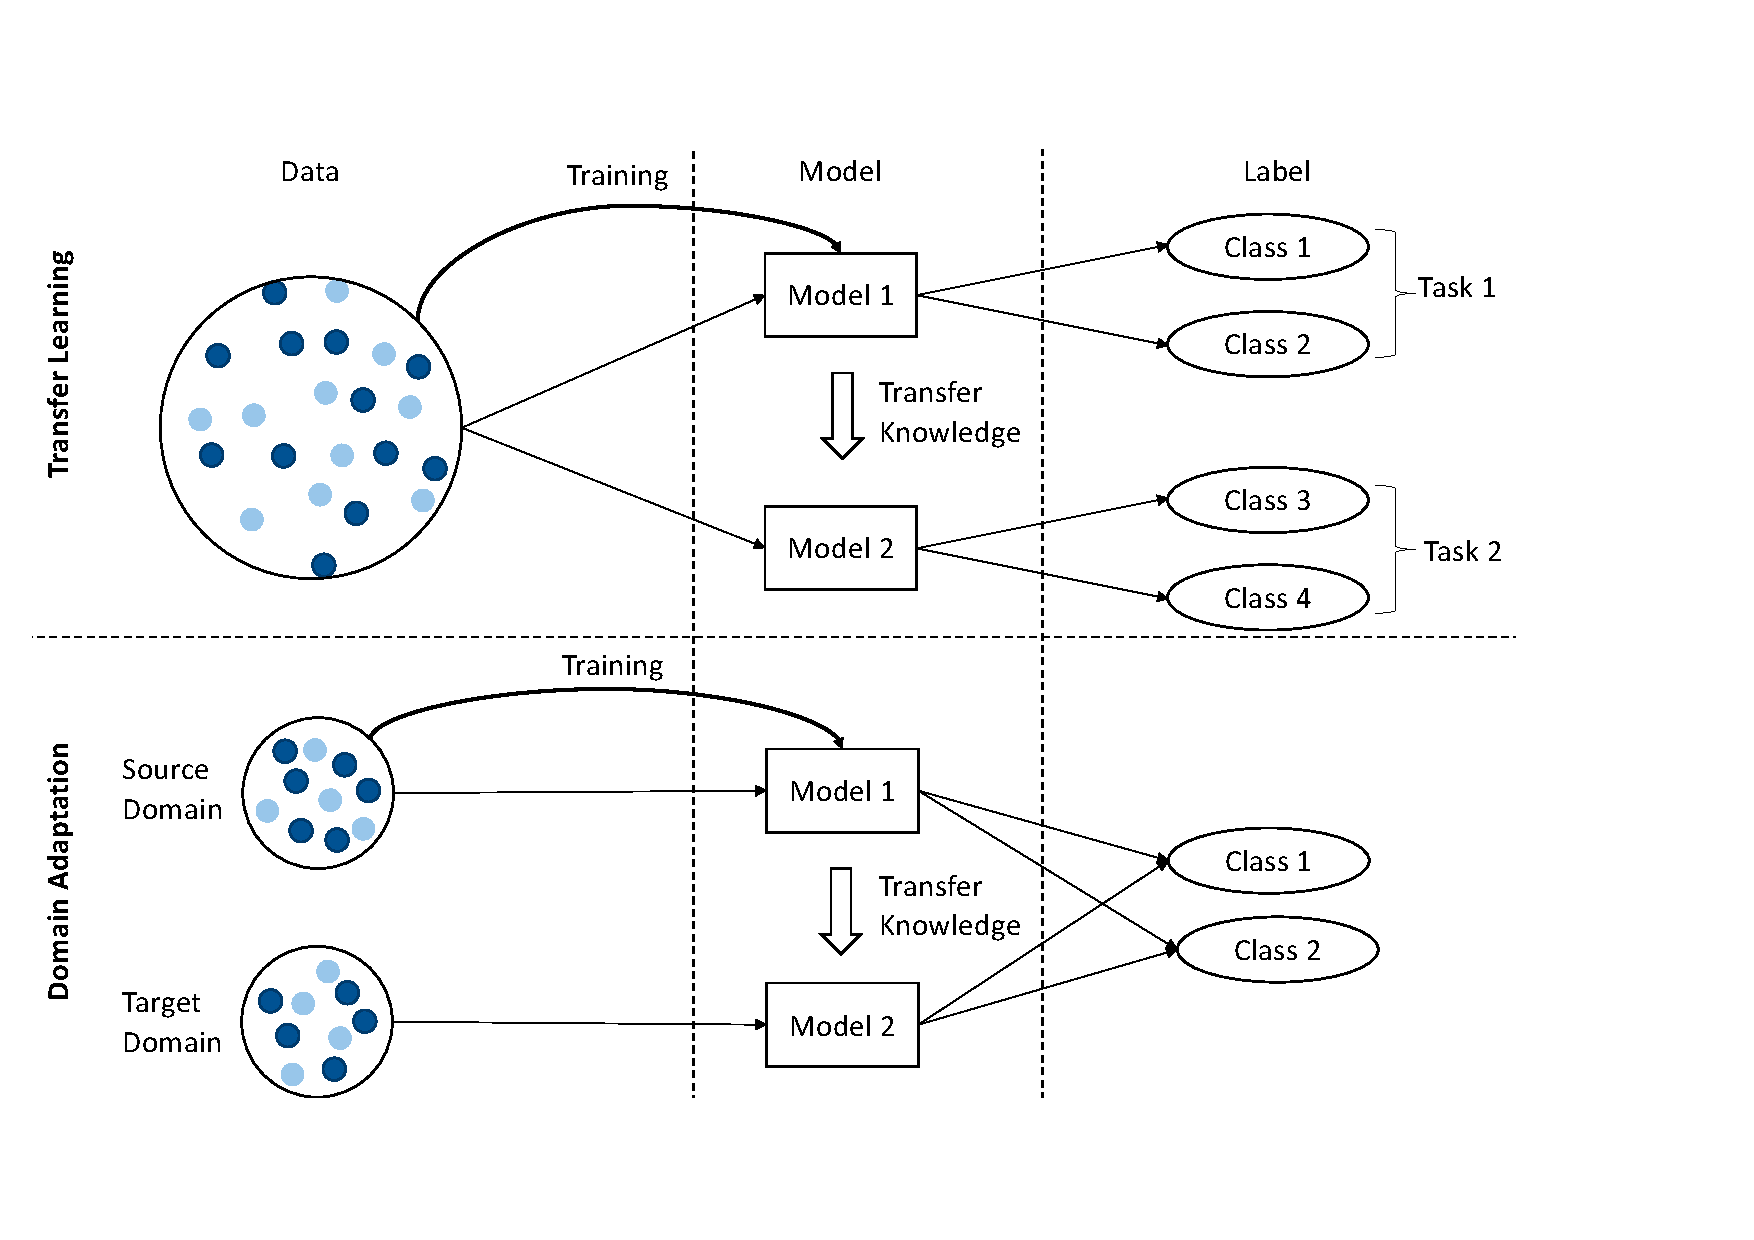
\includegraphics[width=.8\textwidth]{domain_adaption_vs_transfer_learning.pdf}
  \caption {Transfer learning vs. domain adaption} \label{fig:domain_adaption_vs_transfer_learning}
\end{figure}


Since the focus of this thesis is to analyze domain adaption approaches, the following passages explain the different aspects of domain-adaption.
\subsection{Notation}
The labeled source domain data is denoted by  $S = {(x_{i}^{s}, y_{i}^{s})_{i = 0}^{i = N_{s}}}$. Generally, the target domain data is separated in labeled $T_{l} = {(x_{i}^{tl}, y_{i}^{tl})_{i = 0}^{i = N_{tl}}}$ and unlabeled data $T_{u} = {(x_{i}^{tu})_{i = 0}^{i = N_{tu}}}$. Usually, it is assumed that there is a large amount of labeled data in the source and a small amount of labeled data in the target domain: $N_{tl} \ll N_{s}$. In this conext $x_{i}$ is referred as the observation and $y_{i}$ as the corresponding label  \cite{Patel2015}. Depending on the data available during training, one differs between different branches of domain adaption: 
\begin{itemize}
\item \textbf{Semi-supervised domain adaptation}, where a function is trained to use the data from $S$, $T_{l}$
\item \textbf{Unsupervised domain adaptation}, where a function is learned using the data from $S$ and $T_{u}$ \cite{Patel2015} 
\end{itemize}

From a statistical point of view, the source and target domain can be described by the marginal distribution $P(X)$ and conditional distribution $P(Y|X)$. It is required that the data from source and target have the same data space and label space, but the marginal and conditional distribution may differ $P(Y_{s}) \neq P(Y_{t})$ and $P(Y_{s}|X_{s}) \neq P(Y_{t}|X_{st})$ \cite{Qikang2020}

\subsection{Types of Transfer Learning}
Generally, domain adaption approaches can be grouped in four different types \cite{AZAMFAR2020103932}:  

\begin{itemize}
\item \textbf{Instance Weighting Methods} can be used to address this covariate shift problem by integrating weights into a loss function that estimates the discrepancy between source and target. Weighting factors like $\frac{P_{t}(x)}{P_{s}(x)}$ can be used. When a source domain sample has a high probability to be in the target domain, this means that the source domain sample is quite similar to the target domain samples. Samples like that should be strongly included in the training to optimize the model to work well on the target domain data.
\item \textbf{Feature-Based Transfer Learning} has the goal to find a feature space in which the domain discrepancy is reduced. All source and target samples are transferred in the domain-invariant feature space, where the classification of data from both domains works well. Fig. \ref{fig:Domain_adaption_intro} illustrates how feature-based domain adaption can be used to find a cross-domain classifier which accurately separates source and target domain data \cite{Pandhare2021}. 
\item \textbf{Model-Based Transfer Learning} aims to find a classifier trained on the source domain, which can be transferred or fine-tuned to perform well on the target domain.
\item \textbf{Relation-Based Transfer Learning} has the goal to find and utilize similarities between the two domains, which helps to transfer knowledge. 
\end{itemize}

\begin{figure}[H]
  \centering
  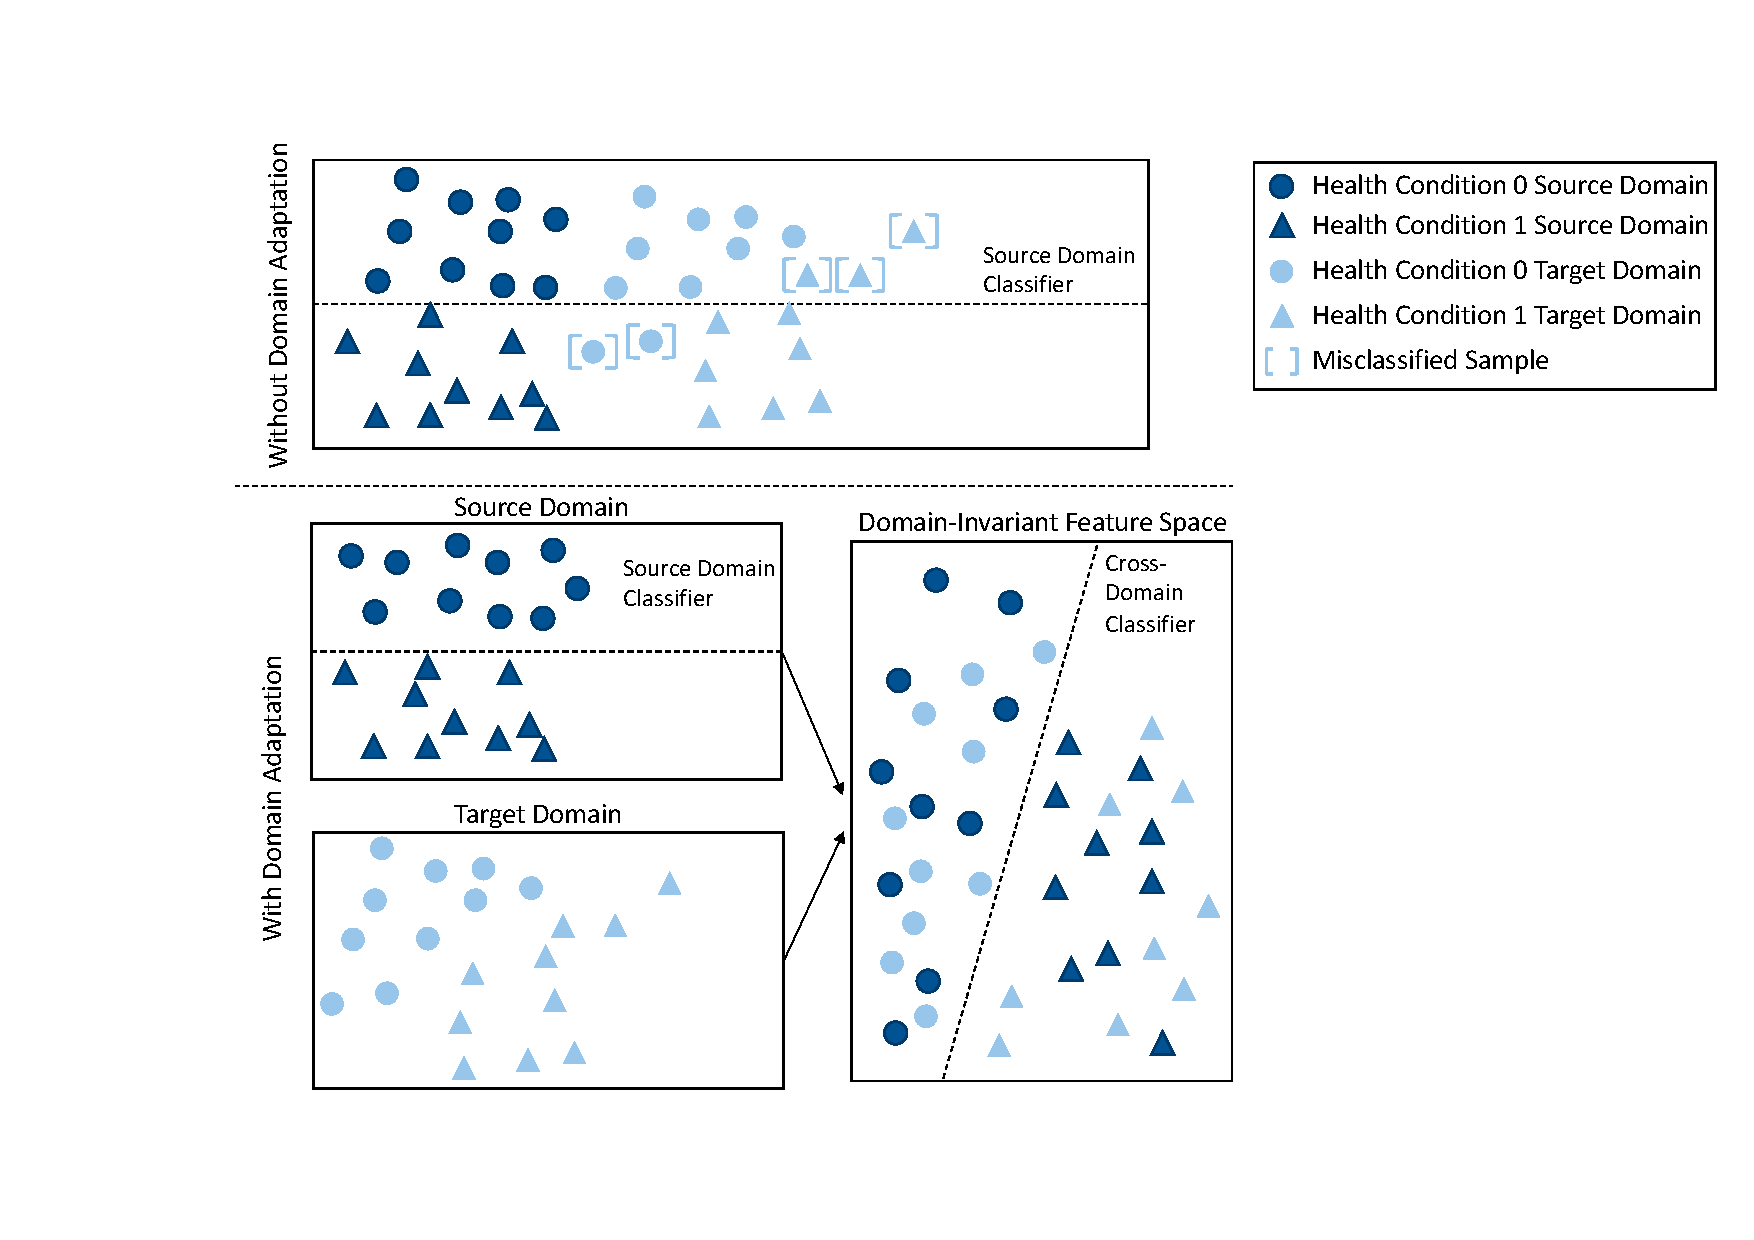
\includegraphics[width=1\textwidth]{domain_adaption_intro.pdf}
  \caption {Domain adaption for PHM based on \cite{Pandhare2021}} \label{fig:Domain_adaption_intro}
\end{figure}


\section{Maximum Mean Discrepancy}
Maximum Mean Discrepancy (MMD) is a criterion which estimates the discrepancy between two distributions. MMD can be used to optimize a neural network such that the distribution discrepancy in its latent feature space is reduced. In the reproducing kernel Hilbert space (RKHS) the discrepancy is measured as squared distance between the distribution kernel embeddings. The distribution discrepancy across domains can be measured in several layers of the neural network. Including this information in the optimization of the model helps to avoid feature transferability degradation \cite{li2020}. 

\begin{align}
    M_{k}(P,Q) = \Bigl|  \boldsymbol{E_{P}}[\Phi(\boldsymbol{X^{s}})] - \boldsymbol{E_{Q}}[\Phi(\boldsymbol{X^{t}})]     \Bigl|^{2}_{Hk}
\end{align}

Hk denotes the RKHS, which is described by the characteristic kernel k and the mapping function $\Phi$. When taking the identity function as mapping function, the discrepancy of the distribution means is measured. When using more complex mapping functions also higher order moments can be matched \cite{Yujia2015}. The distributions of the source domain $X^{s} = \{{x}_{i}^{s}\}_{i=0,...,n_{s}}$ and target domain $X^{t} = \{{x}_{i}^{t}\}_{i=0,...,n_{t}}$ in the latent feature space of interest are represented by P and Q. $\boldsymbol{E_{P}[.]}$ is the expected value of the source distribution and $\boldsymbol{E_{Q}[.]}$. The kernel choice is of great importance when applying MMD for optimizing neural networks. For this reason, it makes sense to combine several kernels to profit from their individual performance:

\begin{align}
    k(\boldsymbol{X^{s}}, \boldsymbol{X^{t}}) = \sum_{i=0}^{N_{k}} k_{\sigma_{i}}(\boldsymbol{X^{s}}, \boldsymbol{X^{t}})
\end{align}

$N_{k}$ denotes the number of kernels used in the RKHS and $k_{\sigma_{i}}$ represents one individual RBF kernels  \cite{li2020}. Other kernels like linear kernels could be used, but current research shows that RBF kernels usually perform best \cite{AZAMFAR2020103932}.


\section{Non-Stationary Signal Analysis for Prognostic and Health Management}
Non-stationary signal analysis, which is a method to investigate signals with changing statistical properties, is one of the main topics in the field of machinery fault diagnosis. Signals can contain multiple frequencies and amplitudes which might change over time. Traditional signal analysis techniques make stationary assumptions. When applying those to non-stationary signals, solely statistical averages in time or frequency can be extracted \cite{FENG2013}. Therefore, the demand for analysis methods, which allow to ascertain features of non-stationary signals, is increasing. Such methods seem promising for extracting health related information from machine data. Time–frequency representations (TFRs) are techniques to transform non-stationary signals in a two-dimensional time-frequency planes, where each value describes the dominance of a specific frequency at a certain point in time. All TFRs, which fulfill this idea of linearity and superposition, are called linear TFRs. The two most popular linear TFRs are the short-time Fourier and the Wavelet transform \cite{Hlawatsch1992}. 


\subsubsection{Short-Time Fourier transform}
Short-time Fourier transform (STFT) is a method which adds a time variable to the traditional Fourier spectrum. This allows to investigate variations in the signal's spectrum over time. STFT assumes the spectrum to be constant during a short time window. For each such window a Fourier spectrum is obtained. The time related changes are measured between consecutive window snapshots in time. The process is mathematically expressed in the following:  
\begin{equation}
    STFT_{x}(t,f) = \int_{- \inf}^{+ \inf}x(\tau) w(\tau -t) exp(-j2\pi f \tau),
\end{equation}
where  $w(\tau -t)$ is the window function centered around t, which is multiplied with the signal $x(t)$. Specific window functions are defined to separate the signal. Shifting the window over the signal and applying the Fourier transform $exp(-j2\pi f \tau)$ to each window, generates a local frequency spectrum of the signal for different points in time t \cite{FENG2013}. The time-frequency resolution is defined by the windowing function and the window length. STFT suffers from a trade-off between high resolution in time or frequency. The optimum window length will depend on the main interest behind the signal analysis. For accurate time domain information the window size needs to be reduced and for frequency domain information increased. STFT  decomposes the signal in existing sinusoidals and determines it's frequency and phase for a local part of the signal \cite{Hlawatsch1992}. 

\subsubsection{Wavelet Transform}
The Wavelet transform decomposes the signals in several wavelets. A wavelet is a wave-like oscillation, which is described by its function, location and scale. The location defines where the wavelet overlaps with the signal and the scale defines how much squished (small scale) or stretched (big scale) the wavelet is \cite{Shawhin2020}. The convolution of the wavelet and the signal is mathematically expressed as following:
\begin{equation}
    WT_{x}(t,a) = \frac{1}{\sqrt{a}} \int_{- \inf}^{+ \inf} x(\tau) \psi(\frac{\tau -t}{a}) d \tau,
\end{equation}
 where $x(t)$ is the signal and $\psi(\frac{\tau -t}{a})$ the wavelet. In this case $a$ is the scaling factor, $t$ the time shift and $\frac{1}{\sqrt{a}}$ a normalization factor to maintain the energy conservation \cite{FENG2013}. Different wavelet bases $\psi(t)$ can be convolved with the signal, which allows to analyze the signal for different patterns \cite{Shawhin2020}. Possible wavelet bases are the Gaussian, Morlet, Shannon, Meyer, Laplace, Hermit, or the Mexican Hat wavelets in both simple and complex functions \cite{Verstraete2017}. This enables a more extensive, flexible and detailed analysis. The wavelet transform can be adapted to extract patterns which are especially relevant for a PHM task. In fig. \ref{fig:ricker_wavelet} Ricker wavelets with different scales and locations are visualized. Wavelet transforms can extract local spectral and temporal information in parallel \cite{Shawhin2020}.


\begin{figure}[H]
  \centering
  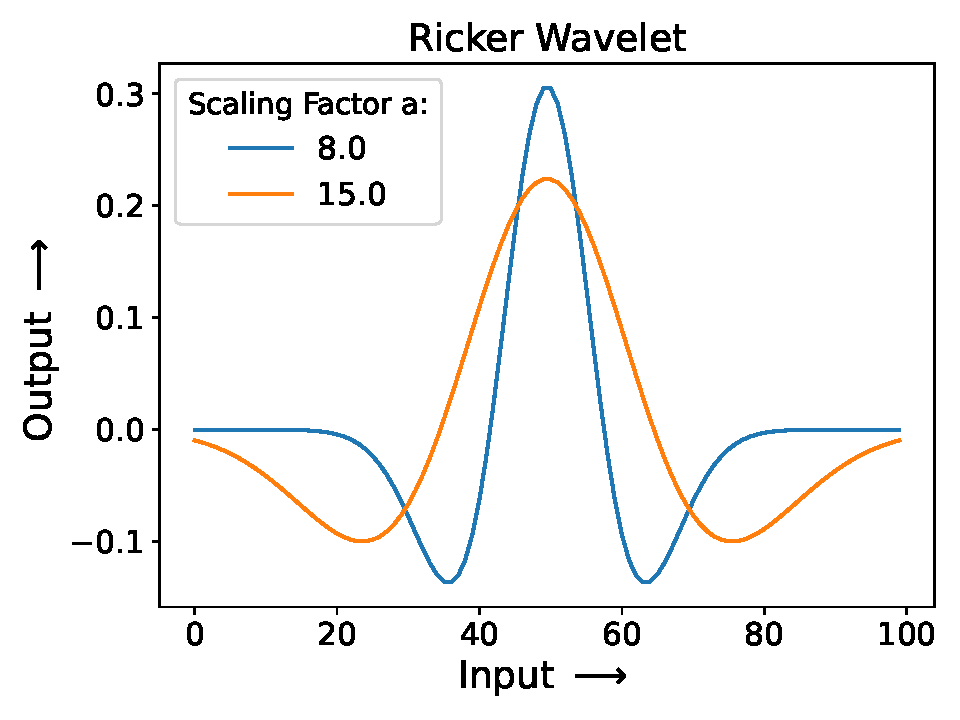
\includegraphics[width=.47\textwidth]{preprocessing_transform/Ricker_Wavelet_Scaling.pdf}
  \hspace{.1cm}
  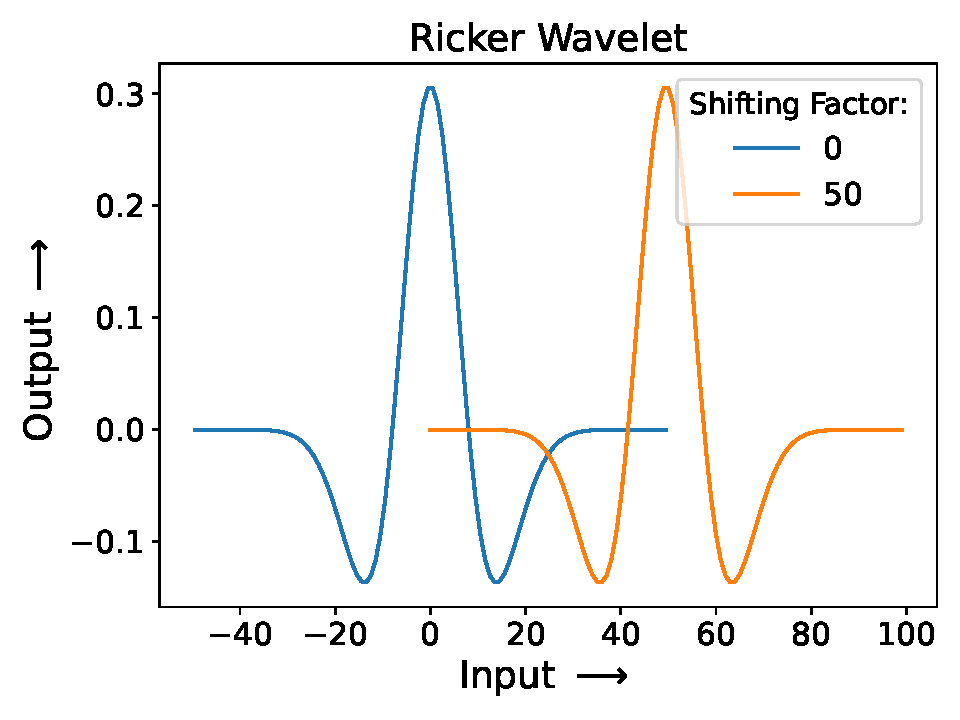
\includegraphics[width=.47\textwidth]{preprocessing_transform/Ricker_Wavelet_Shifting.pdf}
  

  \caption{Ricker wavelet}
  \label{fig:ricker_wavelet}
\end{figure}

\subsubsection{Spectrograms and Scalograms}

 Spectrograms are a graphic representation of the STFT and scalograms of the wavelet transform. Spectrograms and scalograms visualize the the squared magnitudes of the previously presented STFT and Wavelet transform. This squared magnitude is loosely interpreted as signal energy \cite{Hlawatsch1992}. The mathematical expressions are presented in the following: 

\begin{equation}
    \begin{aligned}
        SPEC_{x}(t,f) &= |STFT_{x}(t,f)|^{2} \\
        SCAL_{x}(t,f) &= |WT_{x}(t,f)|^{2}, 
    \end{aligned}
\end{equation}

where $STFT_{x}(t,f)$ is the Short-time Fourier transform, $WT_{x}(t,f)$ the wavelet transform, $SPEC_{x}(t,f)$ the spectrogram and $SCAL_{x}(t,f)$ the scalogram \cite{Hlawatsch1992}. This way of representing the system energy in the 2D time and frequency space may reveal useful information from a complex and high-dimensional signal without the need for additional feature extraction. As described before, spectrograms have a fixed frequency resolution that is defined by the windows size. Scalograms on the other hand have a frequency-dependent frequency resolution \cite{Verstraete2017}.


% !TeX root = ../main.tex
% Add the above to each chapter to make compiling the PDF easier in some editors.

\chapter{Related Works}\label{chapter:related_works}
In this chapter, works from the literature are presented, which tackle problems related to the presented PHM task in this thesis. Section \ref{sec:traditional_approaches} discusses traditional PHM approaches for BSDs, which do not apply any domain adaptation. Then, in chapter \ref{sec:domain_adaption_approach}, deep learning based domain adaptation approaches are introduced, which perform health condition monitoring for BSDs and rolling bearings. Finally, section \ref{sec:domain_adaption_CV} presents an advanced domain adaptation approach from the computer vision community.

\section{Traditional Approaches for Prognostic and Health Management}\label{sec:traditional_approaches}

Traditionally, model-based and data-driven models were used for PHM. Model-based methods predict the health condition based on physical models describing the underlying degradation mechanisms. Data-driven methods learn a mapping relationship between the machine's health condition and the monitoring data \cite{DENG2020}. The following presents traditional data-driven and model-based PHM systems for monitoring the health condition of BSDs.

\subsection{Model-Based Approach: Monitoring of Defect Frequencies Calculated from Rolling Bearings and Transferred to Ball Screw Feed Drives}
Lee et al. \cite{Lee2015} proposed a diagnosis system for estimating the flaking degradation of BSD screw shafts. By filtering the machine signals for previously calculated characteristic defect frequencies, the severity and location of the degradation were predicted. Lee et al. developed a testbed containing one BSD and two linear motion guides. An accelerometer was mounted on the BSD nut. The continuous fatigue process was simulated by punching holes with a diameter of 3 mm in the BSD screw shaft. The motor was actuated with a constant velocity while the data was recorded. Harris and McCool \cite{Harris1996} proposed a method to estimate the characteristic defect frequencies of rolling bearings. Lee et al. \cite{Lee2015} extended that method to make it applicable for BSDs. The BSD screw shafts were considered as inner rings and the BSD nuts as outer rings of the rolling bearings. The defect frequencies were calculated from the BSD construction details and relative speeds. The ball pass frequencies of the shaft (BPFS), the ball pass frequencies of the nut (BPFN) and the ball spin frequency (BSF) were considered as defect frequencies: 
\begin{equation}
    BPFS = \frac{1}{120}zn(1+\frac{D_{w}}{d_{m}}cos\alpha),
    \label{eq:defect_frequency}
\end{equation}
\begin{equation}
    BPFN = \frac{1}{120}zn(1-\frac{D_{w}}{d_{m}}cos\alpha),
\end{equation}
\begin{equation}
    BSF = \frac{1}{120}n\frac{d_{m}}{D_{w}} (1-\frac{D_{w}}{d_{m}}cos\alpha)(1+\frac{D_{w}}{d_{m}}cos\alpha) ,
\end{equation}
where $\alpha$ is the contact angle between the ball, nuts and screw shaft, $d_{m}$ is the pitch diameter of the balls, $D_{w}$ is the diameter of a single ball, $n$ is the rotational speed of the BSD screw shaft and $z$ is the number of steel balls. A more detailed visualization of the bearing parameters is shown in figure \ref{fig:defect_frequency_calc}. 

\begin{figure}[H]
  \centering
  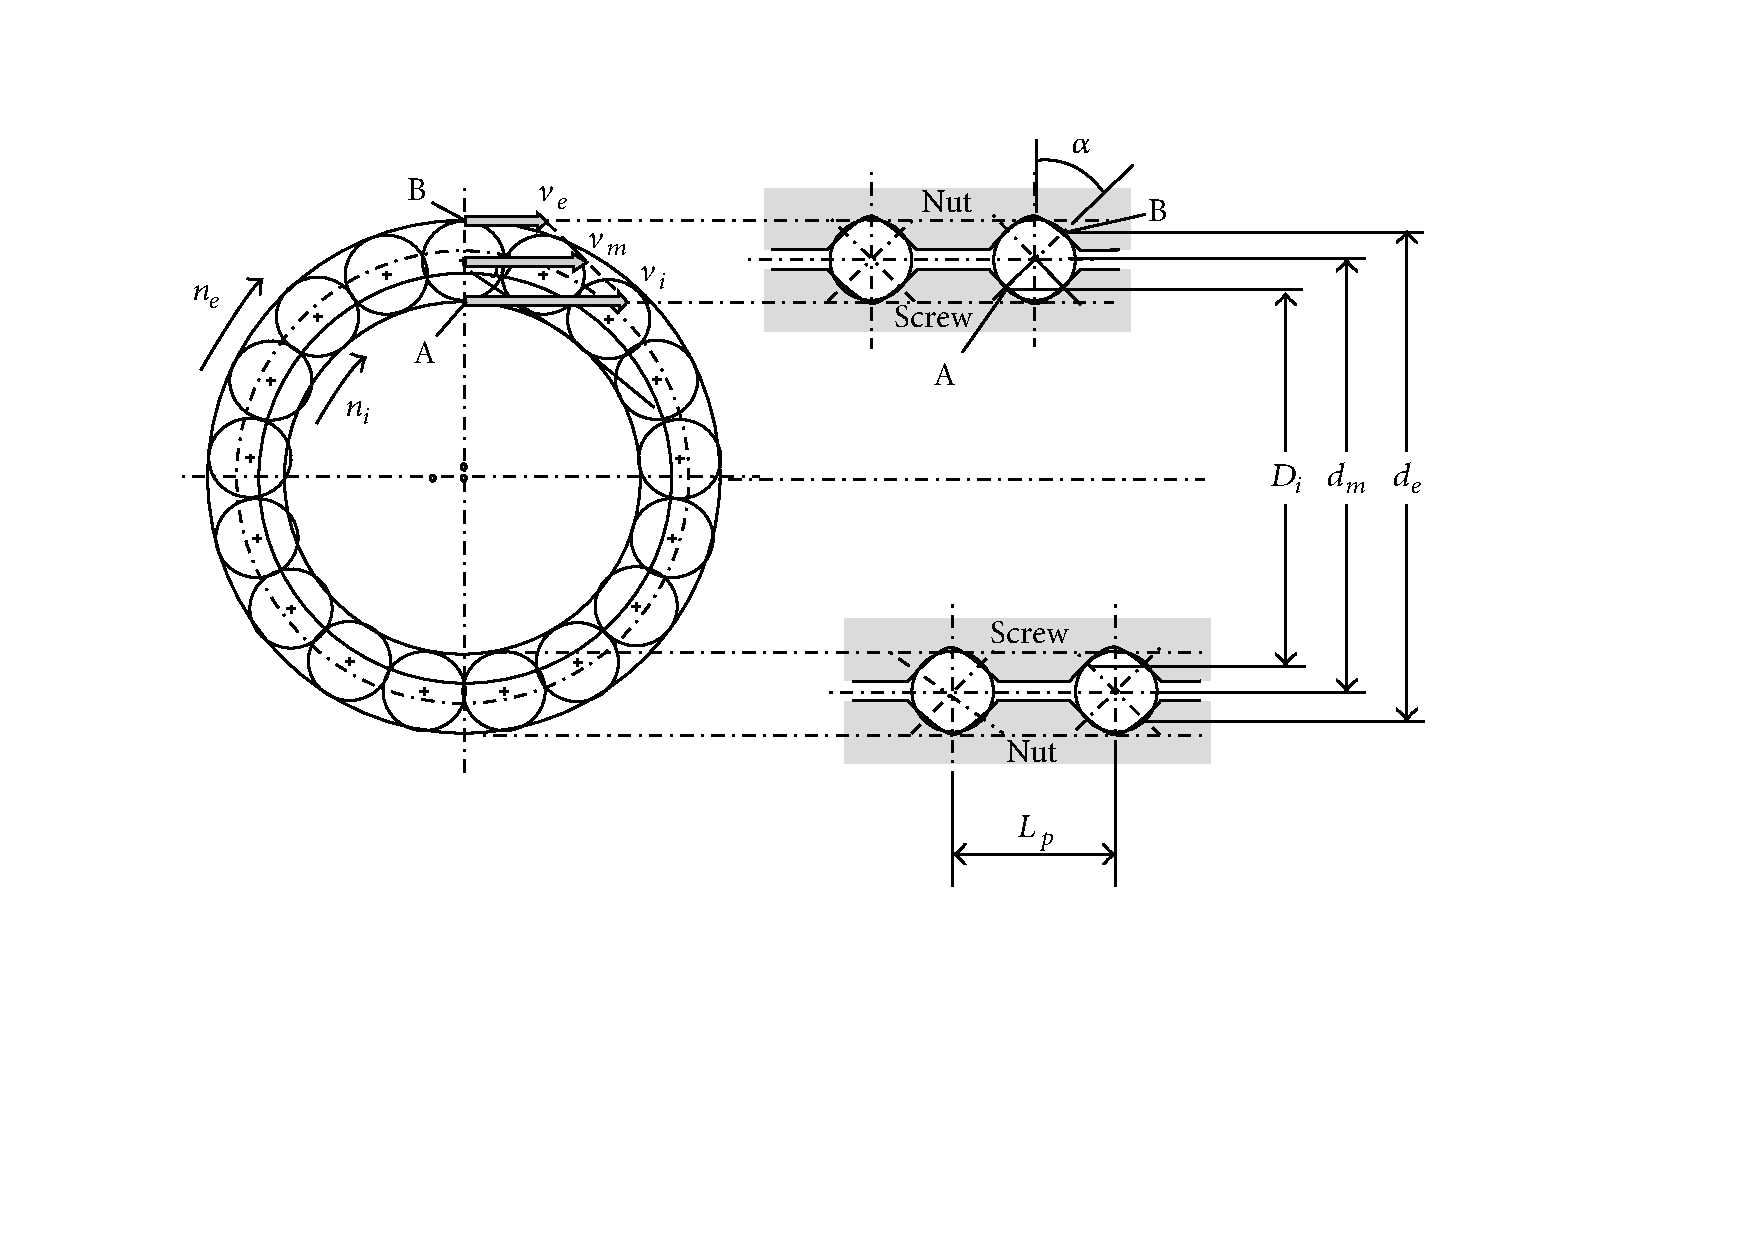
\includegraphics[width=.8\textwidth]{models_state_of_the_art/defect_frequency_calc.pdf}
  \caption{Visualization of the parameters required for the calculation of the defect frequencies \cite{Lee2015}}
  \label{fig:defect_frequency_calc}
\end{figure}

The derived frequencies above are valid for rolling bearings. To correctly apply those to BSDs, $z$ and $d_{m}$ need to be replaced by the effective number of steel balls $z^{'}$ and effective pitch parameter $d_{m}^{'}$, which are defined as follows:

\begin{equation} \label{eq:transfer_RollingBearing_BSD}
    d_{m}^{'} = (L_{p}^{2}+(\pi D_{b})^{2})^{\frac{1}{2}},
\end{equation}
\begin{equation}
    z^{'} = \frac{d_{m}^{'}}{D_{w}}.
\end{equation}

The relation between the regular and effective parameters and the required parameters $L_{p}$ and $D_{b}$ for equation  \ref{eq:transfer_RollingBearing_BSD} are visualized in figure \ref{fig:defect_frequency_transfer}. 

\begin{figure}[H]
  \centering
  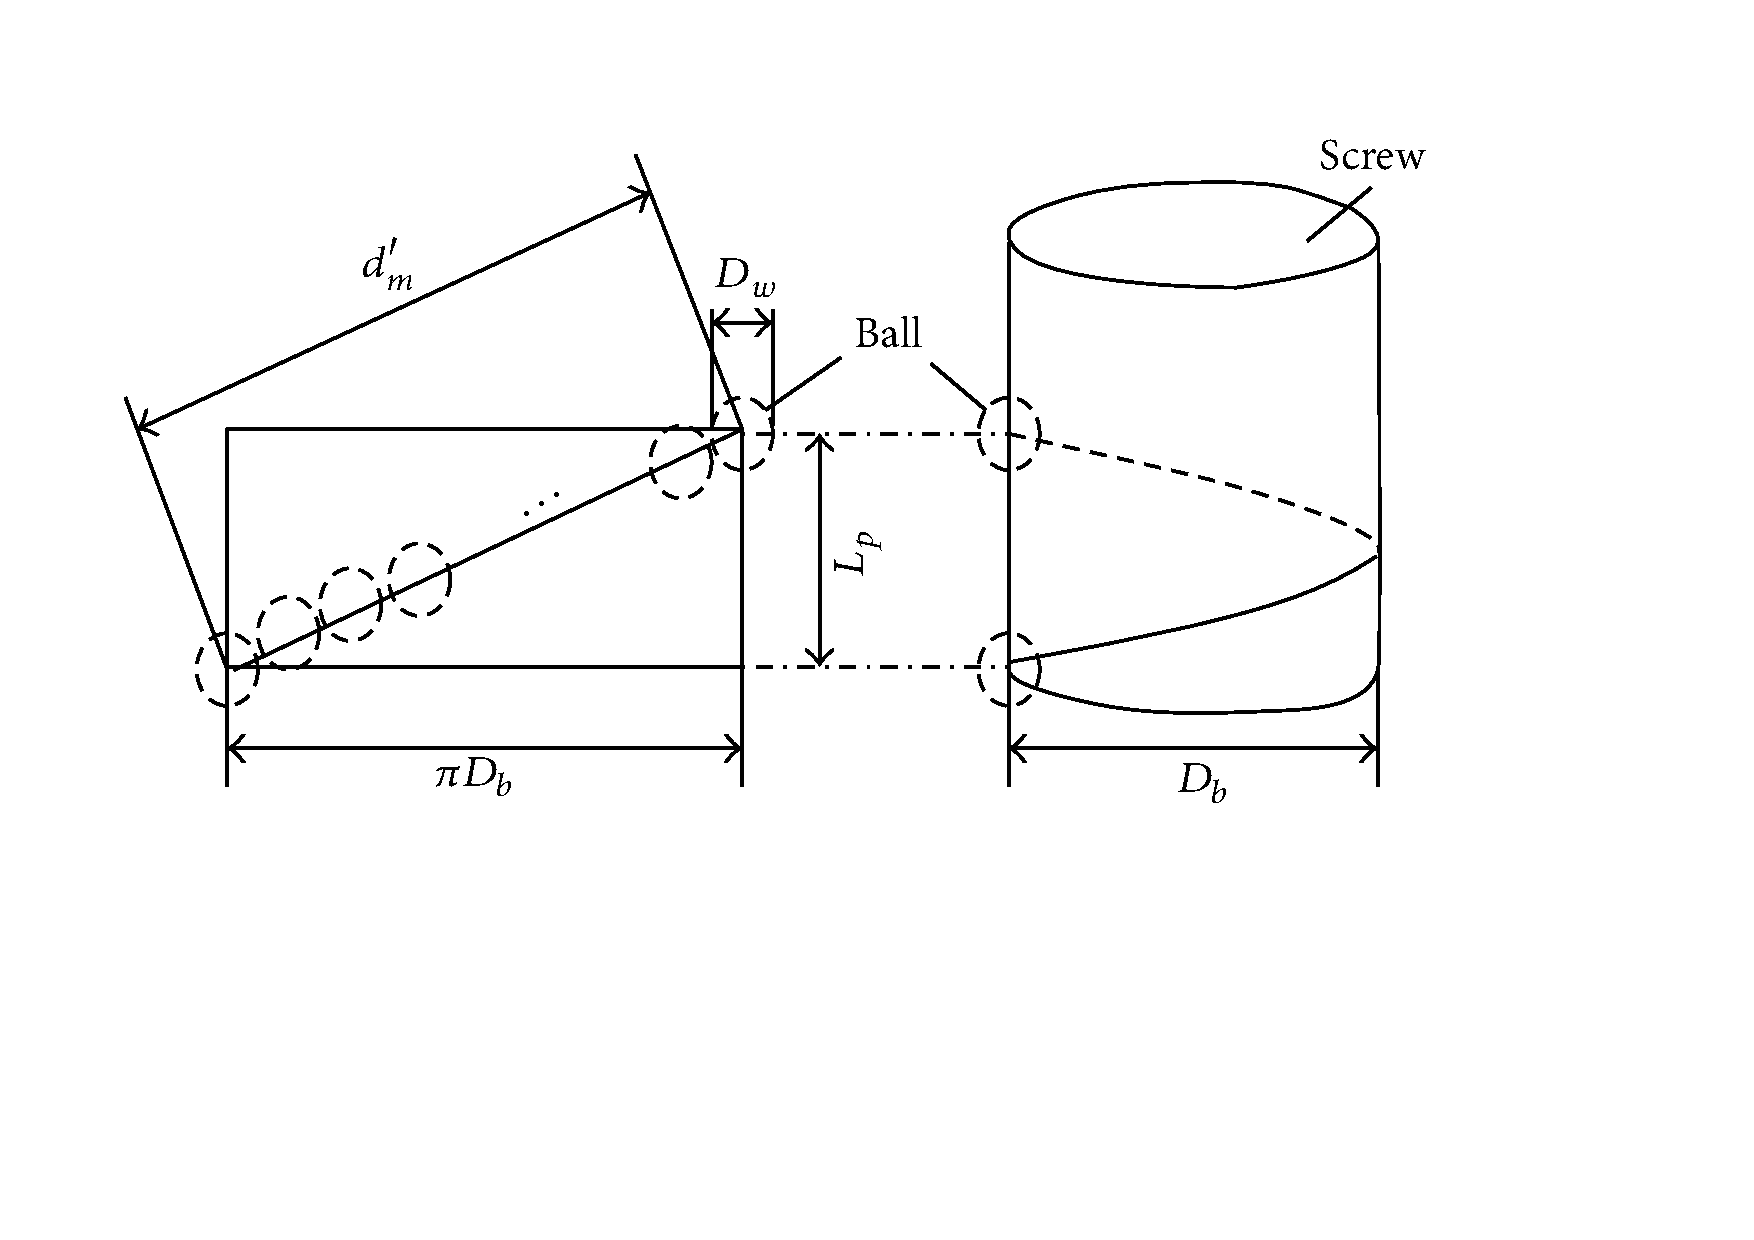
\includegraphics[width=.7\textwidth]{models_state_of_the_art/defect_frequency_transfer.pdf}
  \caption{Relationship between the regular and effective parameters required for transferring the calculated defect frequencies to the BSDs \cite{Lee2015}}
  \label{fig:defect_frequency_transfer}
\end{figure}

The BPFS frequency was identified as the most expressive and reliable for supervising the health condition of BSDs. To calculate the BPFS for ball screw feed drives, the equation \ref{eq:defect_frequency} must be combined with the effective pitch parameter $d_{m}^{'}$ and the effective number of steel balls $z^{'}$. During testing, the wavelet transform (Daubechies Wavelet (db14) function) was used to transform the machine signals in the two-dimensional time-frequency domain. The BSD's degradation status was monitored by supervising the magnitude of the calculated defect frequency in the machine signal's time-frequency domain. An alarm was triggered when the degradation was not acceptable anymore. The time-related information was an indicator of the defect location. The frequency-related information provided information about the degradation extent of the BSD \cite{Lee2015}. The proposed approach during testing is visualized in figure \ref{fig:defect_frequency_model}. 


\begin{figure}[H]
  \centering
  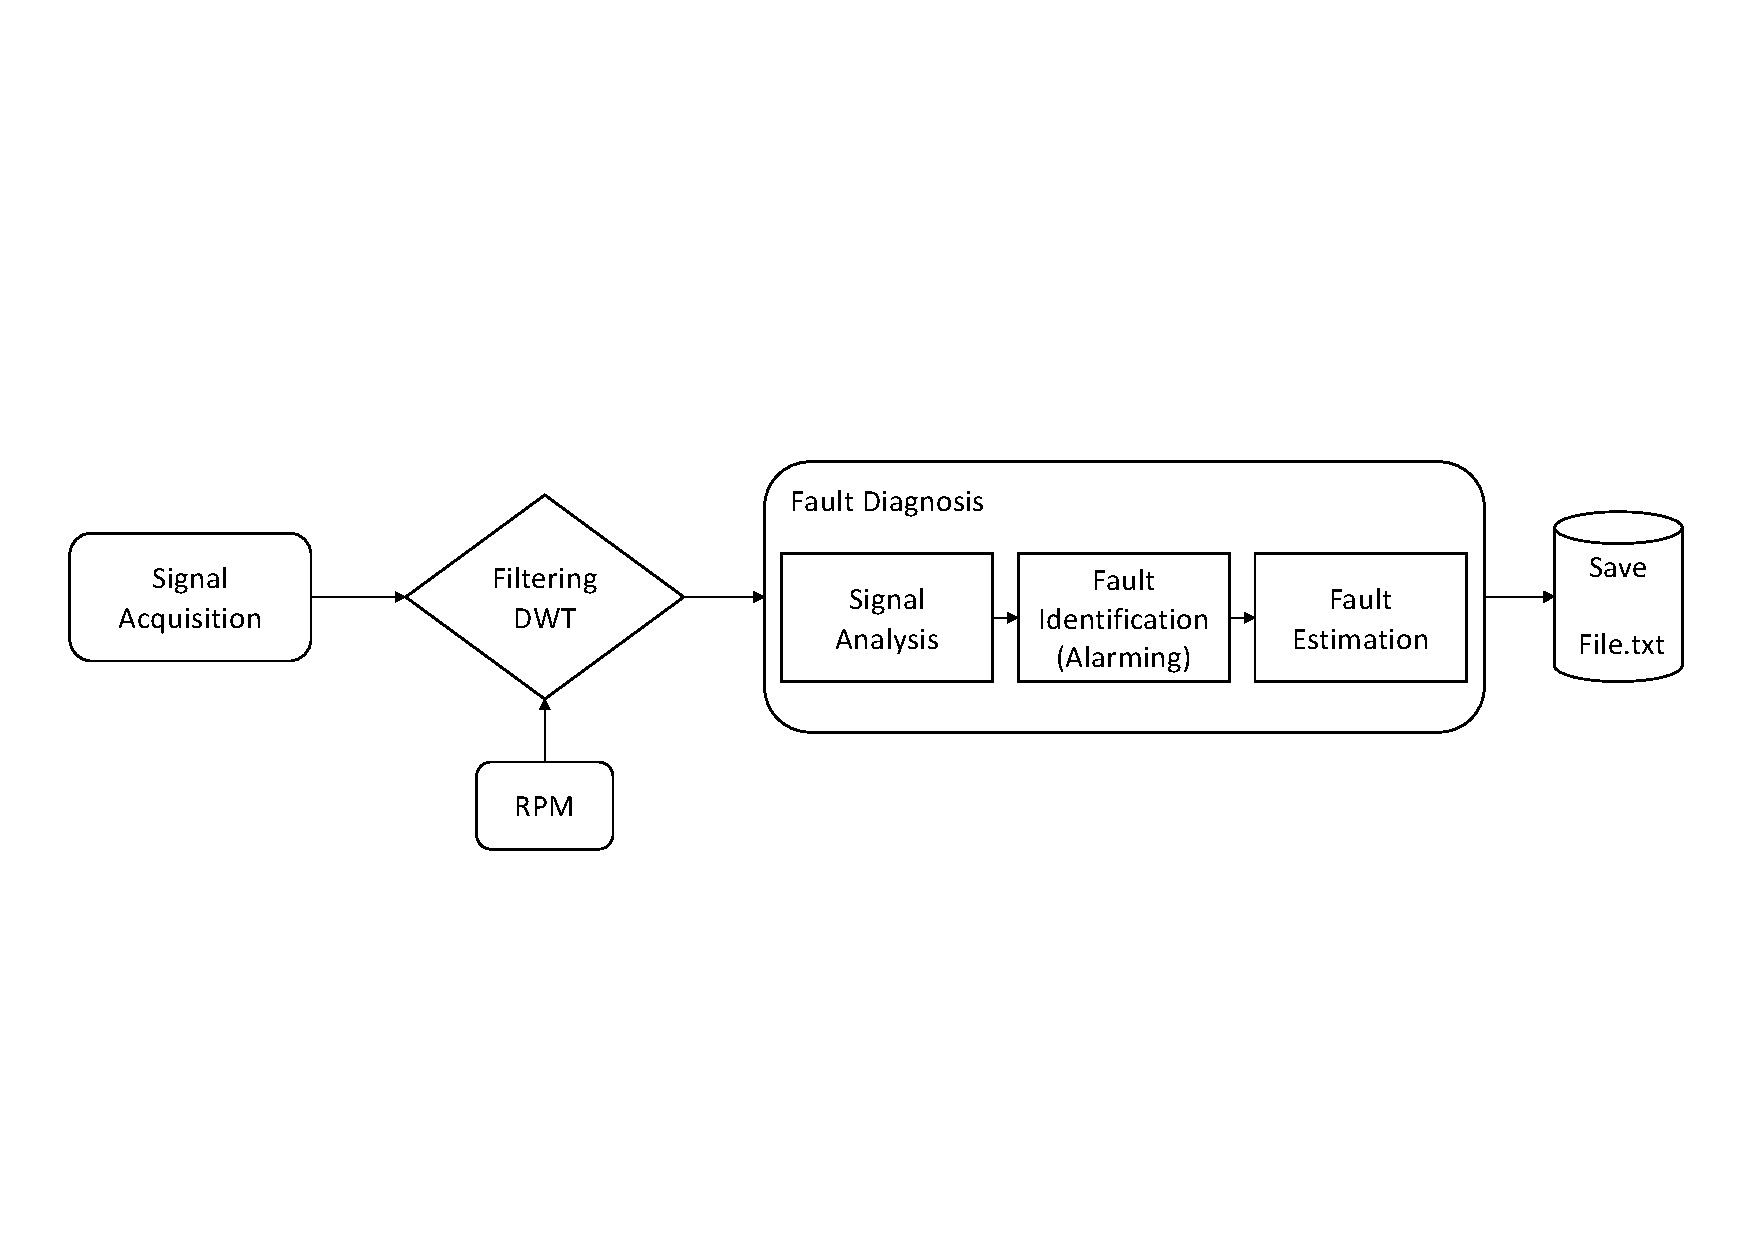
\includegraphics[width=1\textwidth]{models_state_of_the_art/defect_frequency_model.pdf}
  \caption{Failure diagnosis system during testing based on \cite{Lee2015}}
  \label{fig:defect_frequency_model}
\end{figure}

\subsubsection{Conclusion}
Lee et al. \cite{Lee2015} assumed that defects and degradation are mainly subjected to rolling friction. Such simplifying assumptions are often made when developing model-based PHM systems. In reality, the balls in the BSDs are rotating, revolving, and sliding \cite{Lee2015}. These highly complex processes make accurate degradation modeling, which is essential to achieving a good PHM performance, more challenging. In data-driven PHM systems, the correlation between the machine data and the degradation patterns can be learned automatically \cite{ZHAO2019213}. Therefore, these systems can be adapted to monitor different degradation types and corresponding levels by selecting expressive signals and defining appropriate health condition classes. In comparison, Lee et al. \cite{Lee2015} had to adhere to the defect frequencies developed by Harris et al. \cite{Harris1996}, which were limited to the flaking degradation of BSDs. Therefore, adapting the diagnosis system proposed by Lee et al. \cite{Lee2015} to monitor other degradation types is nearly impossible. Furthermore, different operational conditions of the machine might influence the dominance of the characteristic defect frequencies in the vibration signal.
Even in the experiments executed on the simplified testbed, Lee et al. \cite{Lee2015} observed other distinct frequencies coming from significant electrical noise. The monitoring task could become more challenging if vibrations from other parts of the machine disturb the machine signals. This becomes particularly relevant when applying the developed approach to monitoring real-world machines, where the mutual influence of different machine parts is especially strong. Apart from that, the BSD vibration signals were recorded by an accelerometer mounted on the BSD nut \cite{Lee2015}. The BSD nut is a highly fault-critical but also a very impractical sensor location for real-world use \cite{Pandhare2021}. It is questionable how this method would work with vibration signals recorded from less fault-critical sensor locations. Additionally, finding all parameters to calculate the defect frequencies may require copious measuring and testing. Often these parameters change throughout the lifetime of the BSDs. Despite the rolling diameter being reduced due to degradation, it was still used as a constant parameter in the calculation of the BSD’s defect frequencies \cite{Denkena2021} \cite{Pandhare2021}. This indicates that the proposed method is not applicable to monitoring BSDs' health condition over long periods. Only structural differences were considered when transferring the calculated defect frequencies from the rolling bearing to the BSD \cite{Lee2015}. The linear movement of the BSDs was completely ignored, representing a fundamental functional difference between rolling bearings and BSDs. The ongoing degradation was simulated by punching 3 mm diameter holes in the grooves of the BSD screw shaft. Variations in the dimension of these holes were not considered \cite{Lee2015}. This simplified degradation simulation reduces the relevance of the presented results.

\subsection{Model-Based Approach: Ball Screw Feed Drive Preload Estimation Based on a Discrete Dynamic Model}
Nguyen et al. \cite{NGUYEN2019} applied a simplified discrete dynamic model (see figure \ref{fig:Nguyen_discrete_dynamic_model}) to investigate the relation between the preload variations and the dynamic characteristics of BSDs. By estimating the natural frequency of the screw nut in the axial direction from the vibration and current signals, this relationship was then used to predict the preload level of the BSDs. The proposed method was evaluated on a simplified testbed. In the experiments, the preload of the BSDs was changed by a built-in preload adjustment mechanism

\begin{figure}[H]
  \centering
  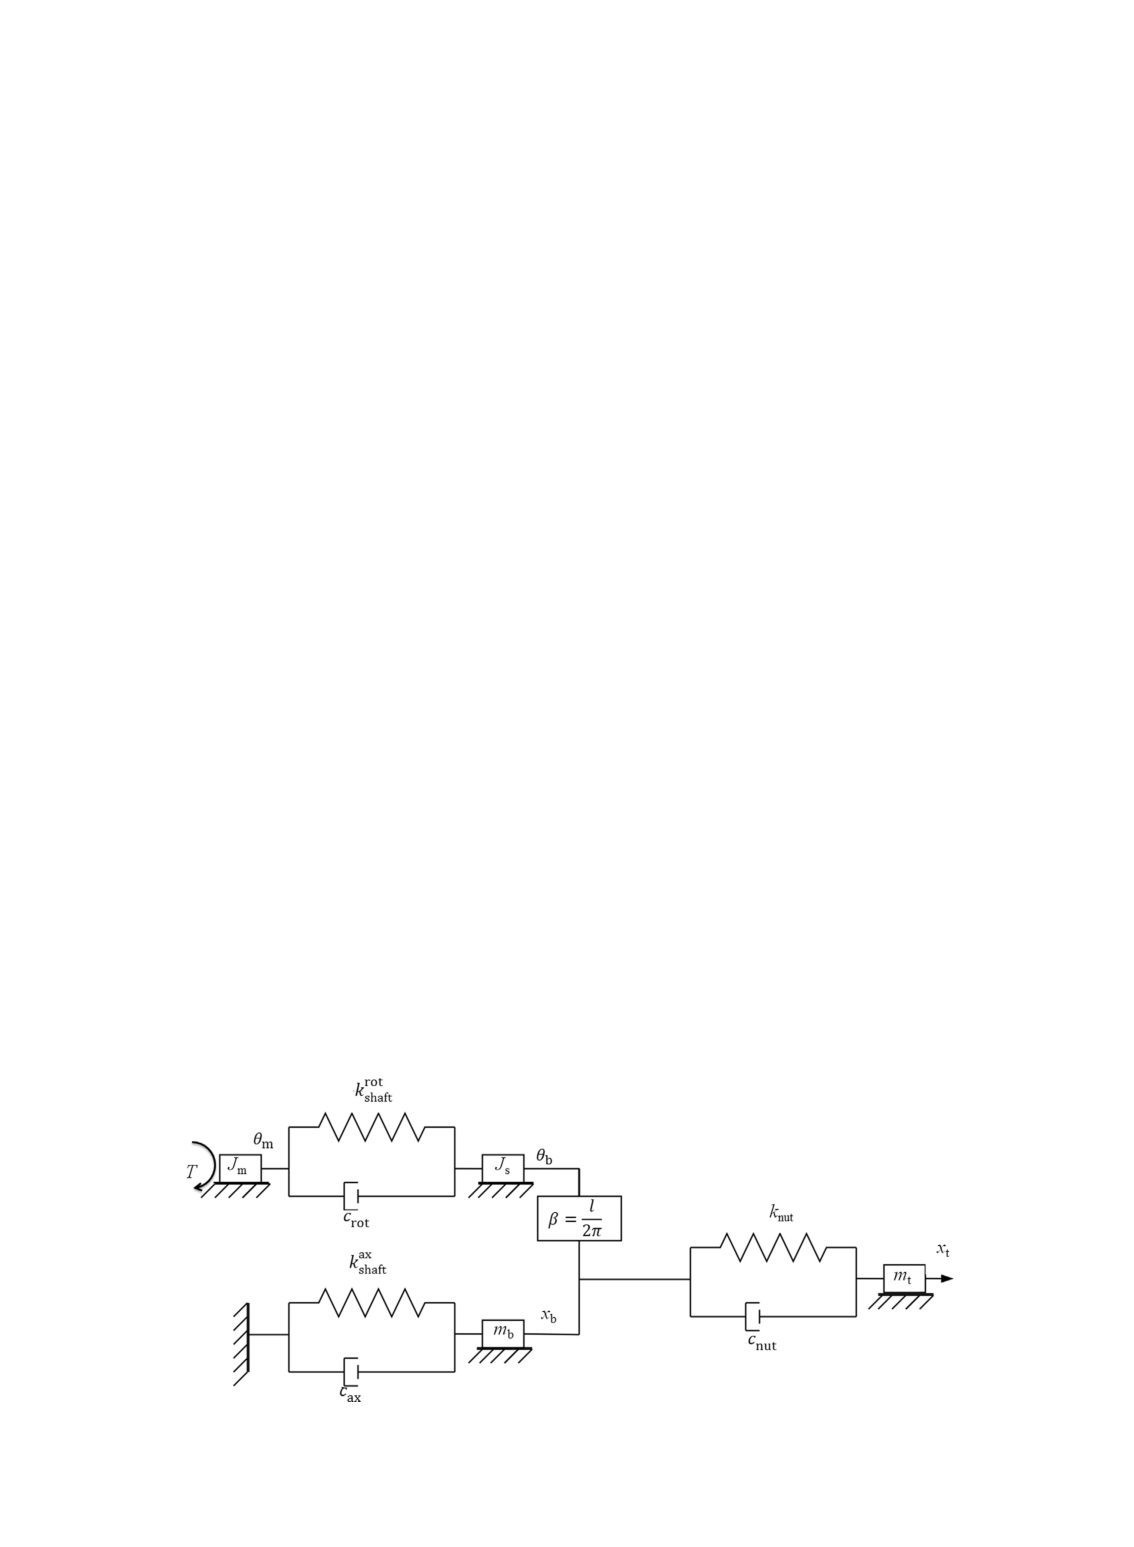
\includegraphics[width=.9\textwidth]{models_state_of_the_art/Nguyen_discrete_dynamic_model.pdf}
  \caption{Discrete dynamic model based on \cite{NGUYEN2019}}
  \label{fig:Nguyen_discrete_dynamic_model}
\end{figure}

According to the discrete dynamic model, the preload variations of BSDs correlate with the screw nut stiffness:

\begin{equation}
    k_{nut}=0.8K(\frac{P}{0.1C_{a}})^{\frac{1}{3}},
\end{equation}

where $P$ is the BSD preload, $C_{a}$ is the BSD screw dynamic load, $K$ is the BSD nut stiffness according to the manufacturer and $k_{nut}$ is the actual BSD nut stiffness. The formula is valid if the BSD preload is less than 10\% of the BSD dynamic load. The axial and rotational stiffness of the BSD screw shaft are determined by the configuration parameters and the working table displacement:
\begin{equation}
    k_{shaft}^{ax}=\frac{EA}{x_{t}}=\frac{\pi}{4x_{t}}d_{minor}^{2}E,
\end{equation}
\begin{equation}
    k_{shaft}^{rot}=\frac{\pi}{32L}d_{minor}^{4}G,
\end{equation}
 where $A$ is the cross sectional area of the BSD screw shaft, $E$ the Young’s modulus, $d_{minor}$ the screw diameter, $G$ the shear modulus, $L$ the screw shaft length and $x_{t}$ the working table displacement. The total axial stiffness of the BSD is composed of several other rotational and axial stiffness:
 \begin{equation}
    \frac{1}{k_{ax}}=\frac{1}{k_{shaft}^{ax}}+\frac{1}{k_{bearing}^{ax}}+\frac{1}{k_{nut}^{ax}}+\frac{1}{k_{bracket}^{ax}}+\frac{1}{\frac{k_{shaft}^{rot}}{\beta^{2}}},
\end{equation}
where $k_{shaft}^{ax}$ is the axial stiffness of the screw shaft, $k_{shaft}^{rot}$ the rotational stiffness of the screw shaft, $k_{bearing}^{ax}$ the axial stiffness of the supporting bearing, $k_{nut}^{ax}$ the axial stiffness of the screw nut and $k_{bracket}^{ax}$ the axial stiffness of the bracket. From there, the axial natural frequency can be calculated based on the axial stiffness $k_{ax}$ and the sum of all masses in the ball screw system $\sum M$:
\begin{equation}
    f\approx\frac{1}{2\pi}\sqrt{\frac{k_{ax}}{m_{table}+m_{screw}+m_{nut}+m_{bracket}}}=\frac{1}{2\pi}\sqrt{\frac{k_{ax}}{\sum M}}.
\end{equation}

Finally, the preload of BSDs is related to the axial natural frequency, the mass and displacement of the ball screw system and other configuration parameters:
\begin{equation}
    P=\frac{0.1C_{a}}{\{0.8K[ -\frac{4x_{t}}{\pi d_{minor}^{2}E} -\frac{32\pi^{2}L}{\pi d_{minor}^{4}G}-\frac{1}{k_{bearing}}-\frac{1}{k_{bracket}}+\frac{1}{(2\pi f)^{2}\sum M} ]\}^{3}},
\label{eq:preload_estimation_based_natural_frequency}
\end{equation}
where $C_{a}$ is the dynamic load rating, $K$ the nut stiffness from catalog, $k_{bearing}$ the bearing stiffness and $k_{bracket}$ the bracket stiffness. The axial natural frequency increases with the preload and decreases with the mass of the working table. Based on the formulas derived from the simplified discrete dynamic model, a monitoring system was established, which extracted the axial natural frequency from the machine data and calculated the corresponding BSD preload according to equation \ref{eq:preload_estimation_based_natural_frequency}. The monitoring system can be separated into different processing phases. Firstly, the vibration and motor current signals were measured with a uni-axial acceleration sensor mounted on the screw nut along with three Hall-effect-based current sensors. When the motor speed changed rapidly, the modal modes of the BSD system, including the axial natural frequency, were strongly activated. In these phases, the deformation of the BSD system was strong enough to make its modal modes observable and distinguishable from those of the other components. A trigger was implemented to detect the phases of rapid motor speed change. During those phases, the vibration and motor current signals were recorded and windowed afterward. The FFT transform was applied to extract an auto-spectrum and cross-spectrum for each window. By averaging the FFT transforms from several occurrences at the same positions along the BSD screw shaft, more stable results were achieved, which were less prone to noise. The average frequency response function (FRF) was composed from those spectra. The whole FRF extraction is visualized in figure \ref{fig:Nguyen_frf}. The axial natural frequency is the frequency in the FRF with maximum magnitude, which was found by a peak detection algorithm \cite{NGUYEN2019}.

\begin{figure}[H]
  \centering
  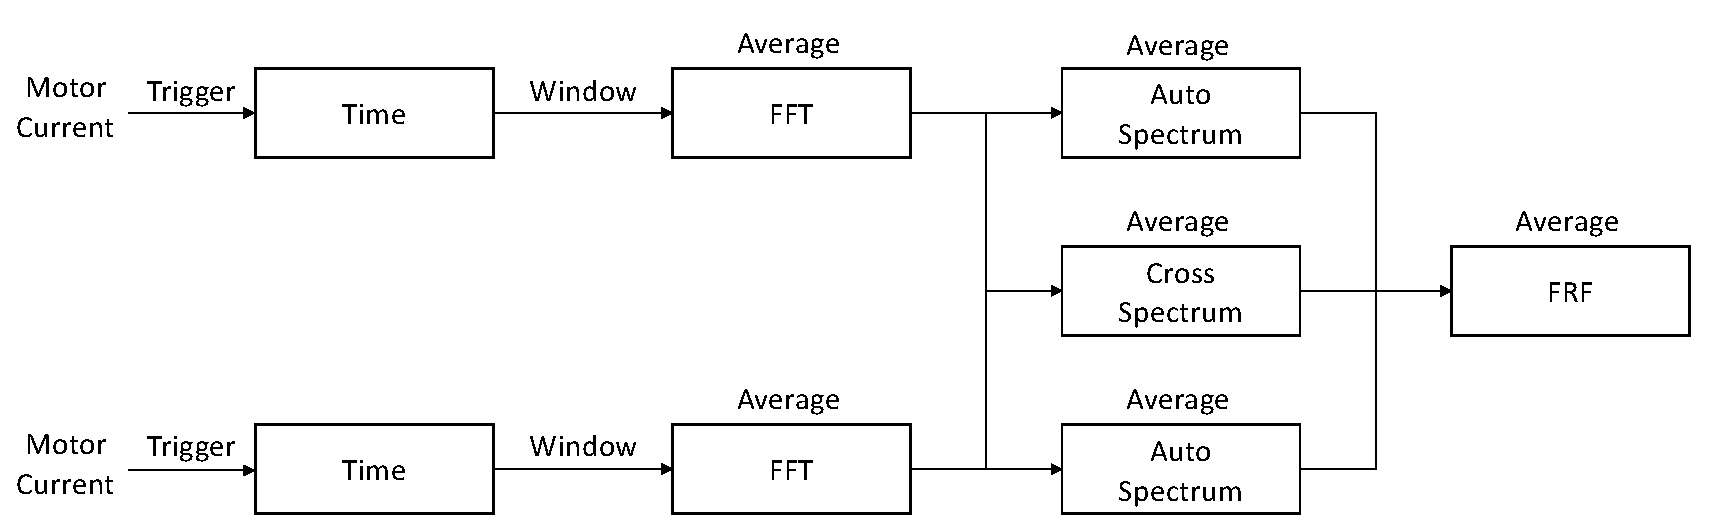
\includegraphics[width=.95\textwidth]{models_state_of_the_art/Nguyen_FRF.pdf}
  \caption{Average FRF calculation based on \cite{NGUYEN2019}}
  \label{fig:Nguyen_frf}
\end{figure}

\subsubsection{Conclusion}
Nguyen et al. \cite{NGUYEN2019} developed a complex inspection procedure to predict the preload of BSDs. The discrete dynamic model presented in figure \ref{fig:Nguyen_discrete_dynamic_model} is the base of the preload prediction. The BSD system was simplified by springs and dampers \cite{NGUYEN2019}. The quality of such prediction systems highly depends on the accuracy of the underlying model and its closeness to the real-world BSD \cite{ZHAO2019213}. The modes of the BSD system were especially activated when the motor changed its velocity rapidly. In this case, the modes of the BSD were dominant enough to become visible and distinguishable from those of other components \cite{NGUYEN2019}. When inspecting BSDs installed in big industrial machines, vibrations from several other components might disturb the machine signals, making extracting the axial natural frequency more challenging than in the simplified testbed. Furthermore, the working table mass, displacement and axial natural frequency must be estimated while the system is operational \cite{NGUYEN2019}, which can be extra laborious for big industrial machines. Since the operational conditions of industrial machines change, these parameters can not be assumed to stay constant. Therefore, re-estimating the required parameters is necessary for each inspection. Only if that is done correctly will the established relationship between the axial natural frequency, the displacement of the working table and the preload of the BSD be reliable. During the experiments in the isolated and simplified BSD testbed, the system partially failed to detect expressive operational phases for estimating the axial natural frequency \cite{NGUYEN2019}. Implementing a trigger to find such phases in big industrial machines might be even more difficult. Nguyen et al. \cite{NGUYEN2019} emphasized that at least ten trigger events from each position along the BSD screw shaft are required to accurately average the FRF in practical applications. Collecting this large amount of trigger events involves substantial effort and time. Equally to the work of Lee et al. \cite{Lee2015}, the BSD nut was used to record the vibration signal. The extraction of the axial natural frequency from signals recorded by sensors in less fault-critical sensor locations was not tested. The physical degradation of the shaft and ball surfaces was neglected in the experiments.

\subsection{Data-Driven Approach: Sensor Fusion of Multiple Hand-Crafted Statistical Features}

Denkena et al. \cite{Denkena2021} presented a method to monitor the preload of BSDs. Firstly, several hand-crafted statistical features were extracted from the machine signals. Afterwards, each feature was rated by its robustness and statistical significance. The most promising features were selected and fused based on the principal component analysis (PCA). In the end, decision trees solved the classification task. A testbed consisting of a single BSD and linear guideways was used to evaluate the proposed approach. The preload loss was simulated by installing ball sets with different oversizes. The internal controller provided internal control signals and three uniaxial acceleration sensors measured the system's vibration. The machine data was recorded during a constant feed rate over the whole length of the test bench. The proposed PHM method can be separated into four steps:

\begin{itemize}
    \item \textbf{Data acquisition:} Signals from three uniaxial acceleration sensors and internal control signals were processed simultaneously. The signals were separated into phases of zero acceleration (constant movement of BSD nut on the BSD screw shaft) and non-zero acceleration (direction change movement of the BSD nut at each end of the BSD screw shaft). In the experiments, the ball screw was moved over the whole length of the test bench with various feed rates (6000 mm/min, 11000 mm/min, 17000 mm/min, 20000 mm/min) \cite{Denkena2021}.
    \item \textbf{Feature extraction:} Information about the preload classes were extracted through statistical features (e.g. kurtosis, median, impulse factor, ...). The features were applied to each signal and segment. At this point, the features were unrated. Each feature was evaluated by its robustness and statistical significance. The robustness was measured by the feature's dispersion around the median. After normalizing the feature with the z-score, the significance was estimated by the f-statistics:

    \begin{equation}
        \textbf{Z-score:}\qquad \tilde{x}_{i,j} = \frac{x_{i,j} - \bar x_{i}}{\sigma_{i}},
    \end{equation}
    
    \begin{equation}
        \textbf{F-statistic:}\qquad f = \frac{\sum_{j=1}^{J} i \cdot (\bar x_{j} -\bar x)^{2}/(J-1)}{\sum_{j=1}^{J} \sum_{i=1}^{I} i \cdot (\bar x_{j,i} -\bar x_{j})^{2}/(J \cdot (I-1))},
    \end{equation}

    
    where ${x}_{i,j}$ denotes the feature value j of a sample of class i, $\bar{x}_{i}$ is the feature mean value of class i, ${s}_{i}$ is the feature standard deviation of class i and $\bar{x}$ is the overall feature and class mean value, I and J are the number of all classes and features. Features were seen as eligible for the diagnosing system if the dispersion around the median was smaller than $\pm$ 10 and the f-statistic was higher than a critical value of 10 \cite{Denkena2021}. 
    
    \item \textbf{Principal Component Analysis:} 
    PCA is a method to reduce the dimension of data while retaining most of the information. Principal components are the directions in the feature space, along which the variation of the data is maximal. By using only a few principal components, each sample can be represented by a smaller number of variables \cite{Ringner2008}. By applying PCA, the selected features were merged with the goal of maintaining the robustness and increasing the f-statistics \cite{Denkena2021}.
    
    \item \textbf{Classification:} Decision trees were used to predict the preload class based on the extracted features. Due to its low classification effort and good traceability, decision trees are suitable for that classification task. For each signal and segment, a separate decision tree was used \cite{Denkena2021}. 
\end{itemize}

\subsubsection{Conclusion}
In order to find features that work well for predicting the BSD's degradation status, Denkena et al. \cite{Denkena2021} extracted 1500 features from the signal segments. Extracting, evaluating and fusing this amount of features can become computationally expensive. The performed experiments showed that the suitability of the features strongly depended on the machine's working conditions, classes and signals. The following observations proved these dependencies:
\begin{itemize}
    \item \textbf{Working Conditions}: The features were not able to properly separate the classes on those vibration signals recorded with feed rates higher than 11000 mm/min \cite{Denkena2021}. 
    \item \textbf{Classes}: Certain features, like MAX, RMS and CRE, were only able to separate some of the defined preload classes \cite{Denkena2021}. 
    \item \textbf{Signals}: The robustness and statistical significance of some extracted statistical features depended on the signals \cite{Denkena2021}. 
\end{itemize}
The sensitivity to the machine's working conditions, classes and signals shows the system's low robustness, which makes its real-world use questionable. Furthermore, the features did not show proportional behavior to the physical degradation. When the features MAX and RMS were applied to the acceleration signals, they increased from C3 through C2 to C1, but decreased towards C0 \cite{Denkena2021}. Often deep learning is criticized for its black box principle and lack of understanding of the extracted features. Even though one generally understands the hand-crafted features, the meaning of the extracted information strongly depends on the task and signal. The correlation between those features and the physical degradation is often unknown, which makes such features an equal black box to the features extracted by deep learning models. Generally, one can say that finding a set of features that reliably predict all BSD preload classes demands substantial effort. These features work reliably for specific signals, working conditions and preload classes. If any of those specifications change, the entire system must be completely reconfigured. The physical degradation of the shaft and ball surface was neglected in the experiments \cite{Denkena2021}.

\subsection{Data-Driven Approach: Multi-Level Feature Selection of Multiple Hand-Crafted Statistical Features}
Li et al. \cite{LiPin2018} developed a prognosis system for BSDs, which simultaneously performed fault diagnosis, early diagnosis, health assessment and remaining useful life (RUL) prediction. Since this thesis focuses on the fault diagnosis of BSDs, this chapter is restricted to the processing units related to diagnosis. A testbed was built containing a BSD and horizontal guideways fixed to a concrete base. Instead of manually inserting faults to simulate degradation, it was caused by field use. Figure \ref{fig:level_feature_selection_model} shows the different processing steps and the parallel prediction units for the fault diagnosis, health assessment and remaining useful life (RUL) prediction. Vibration data was recorded by three accelerometers, speed and torque signals were retrieved from the controller \cite{LiPin2018}. 

\begin{figure}[H]
  \centering
  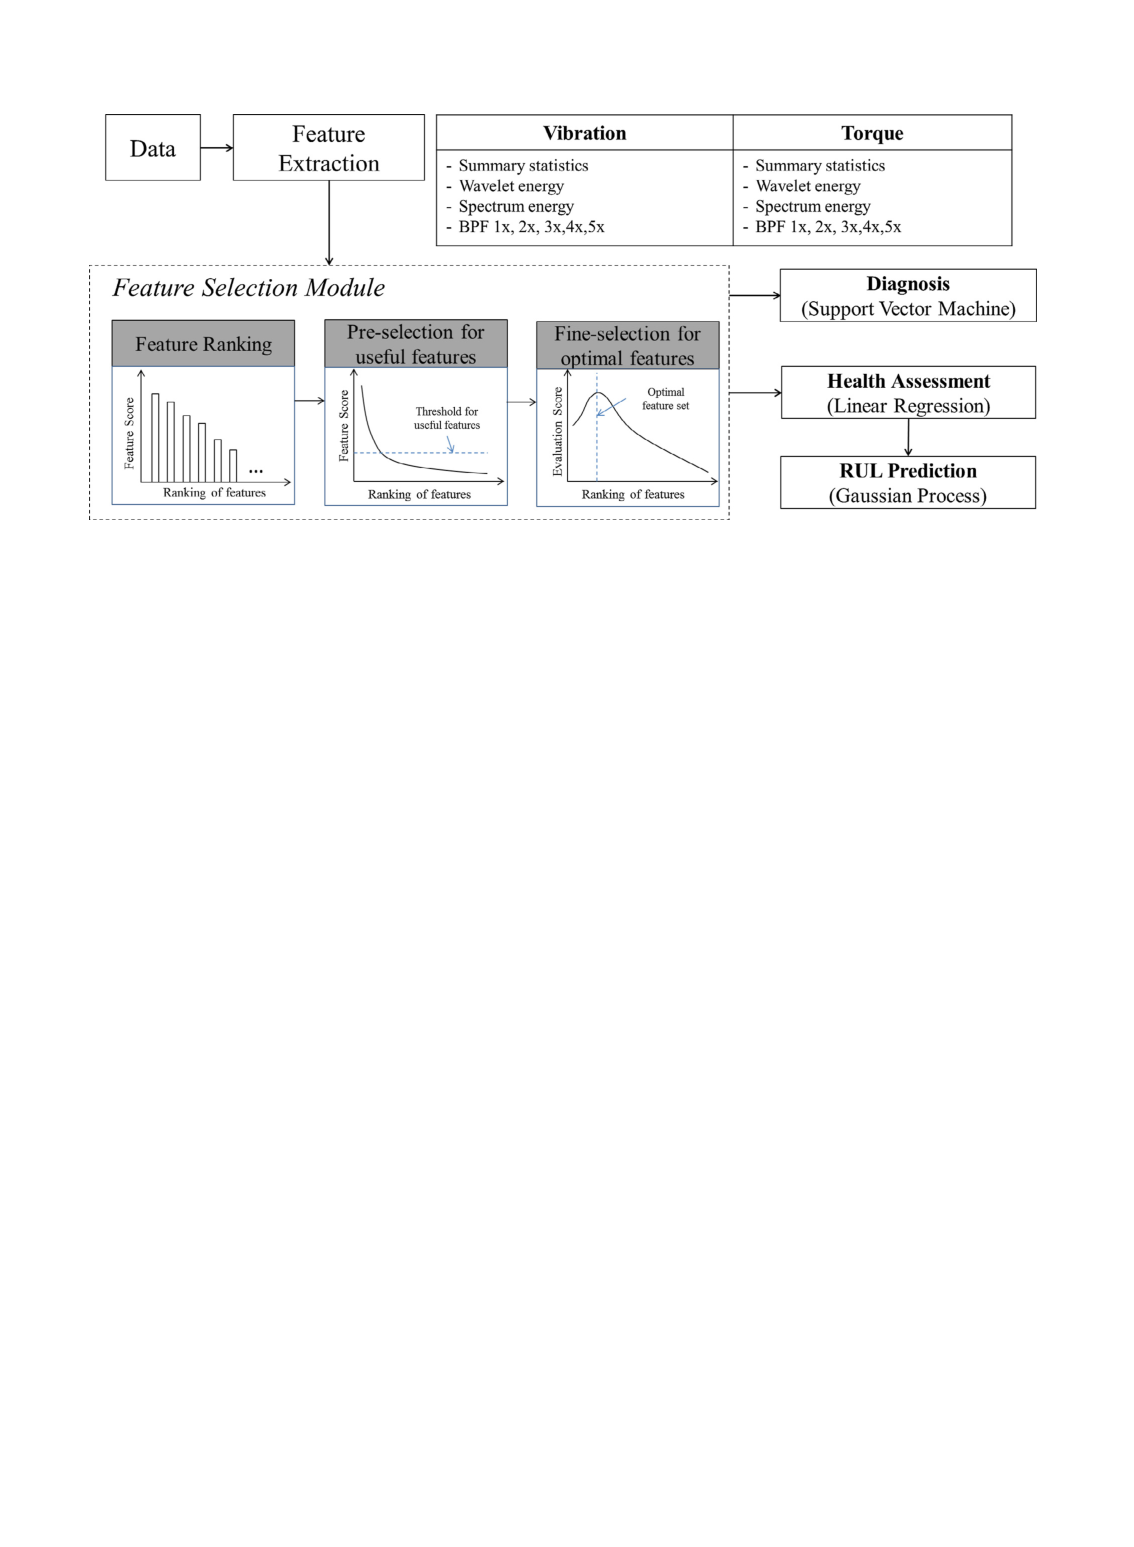
\includegraphics[width=1\textwidth]{models_state_of_the_art/model_multi-level_feature_selection.pdf}
  \caption{Feauture extraction and selection for health diagnosis, health assessment and RUL prediction \cite{LiPin2018}}
  \label{fig:level_feature_selection_model}
\end{figure}

\newpage
In the following, the three diagnosis steps of the proposed PHM system are presented in more detail:

\begin{itemize}
    \item \textbf{Feature Extraction}: The system processed the signals in the time domain, frequency domain and time-frequency domain. The wavelet decomposition (‘db4’ wavelet) was applied to transform the signals. Similarly to Denkena et al. \cite{Denkena2021}, features, such as RMS, mean, variance, kurtosis and skewness, were extracted from the signals in all three domains (time domain, frequency domain and time-frequency domain). Similar to the work of Lee et al. \cite{Lee2015}, the amplitudes corresponding to the calculated ball passing frequency and the ball screw rotation frequency, including its harmonics, were extracted as features for the monitoring system \cite{LiPin2018}.
    \item \textbf{Feature Selection}: In a multi-level feature selection procedure, the extracted features were rated by their suitability for the prognosis task. This process was separated into three stages: primary feature ranking, pre-selection and fine-selection. In order to select expressive features, a hybrid strategy of filter-based (feature ranking and pre-selection) and wrapper-based (fine-selection) methods was applied. Wrapper-based methods rate features by the performance of a classifier using them and filter-based methods by the feature's intrinsic properties \cite{Wald2013}. In the multi-layer feature selection procedure, the search space and search sequence corresponded to the selected features and their corresponding ranking scores found in the previous feature refinement phase. In the primary feature ranking phase, a selection criterion ranked and filtered all extracted features. In the pre-selection phase, the fisher score was applied to refine the previous feature choice:
    \begin{equation}
        S_{c} = \frac{\sum_{k=1}^{C} n_{k}(\mu_{k}^{j}-\mu^{j})^{2}}{\sum_{k=1}^{C}n_{k}(\sigma_{k}^{j})^{2}},
    \end{equation}
    where $C$ defines the number of classes, $n_{k}$ the number of samples in k-th class, $\mu_{k}^{j}$ and $\sigma_{k}^{j}$ the mean and standard deviation of the k-th class and the j-th feature and $\mu^{j}$ the mean of the j-th feature across all classes. For the multi-class classification task, the fisher score is biased. Therefore a fine feature-selection phase was added subsequently. Based on the prediction accuracy of an SVM using the pre-selected features, the final optimal features were chosen \cite{LiPin2018}.
    \item \textbf{Classification}: A second SVM was applied to make the predictions for the diagnosis task. The SVM processed the optimal features found during the fine-selection phase \cite{LiPin2018}. 
\end{itemize}

\subsubsection{Conclusion}
Similar to Denkena et al. \cite{Denkena2021}, Li et al. \cite{LiPin2018} extracted 440 features from the raw data. As mentioned before, the feature extraction and ranking can become computationally expensive when using that many features. Again, the expressiveness of the features strongly depended on the signals and the features did not correlate well with the degradation process \cite{LiPin2018}. In the multi-level feature selection, the SVM-based fine-selection and fisher score-based pre-selection diverged in their feature ranking. Especially the top features found during the pre-selection were rated down by the fine-selection \cite{LiPin2018}. Therefore, the application order of the feature selection methods significantly influenced the final feature choice. Denkena et al. \cite{Denkena2021} also mentioned that finding the empirical threshold for the fisher criterion in a nine-class classification task was challenging. When developing such feature selection modules, one has to select the single feature selection mechanisms, define their application order and find suitable parameters for each of them, which requires substantial effort. Generally, the definition of such feature selection modules strongly influences the performance of the PHM system and is highly dependent on the working conditions, health condition classes and signals. Minor variations in the predefined task specifications will most certainly reduce the performance of such PHM systems or could even make them fail. Using SVMs in the feature selection increases the training effort, which raises the training time and data requirements.

\newpage

\section{Domain Adaptation Approaches for Prognostic and Health Management} \label{sec:domain_adaption_approach}
With the goal of developing robust monitoring systems for complex industrial machines, PHM systems need to become more flexibel, adaptable and intelligent. Inspired by the advances in the computer vision community, domain adaptation and transfer learning approaches have achieved greater popularity for industrial PHM. 

\subsection{Domain Adaptation Approaches for Prognostic and Health Management of Ball Screw Feed Drives}
In the following, deep learning based domain adaptation models for monitoring the health condition of BSDs are presented. Similarly to the method proposed in this thesis, the presented models applied the MMD metric to measure and reduce the domain discrepancy in the latent feature spaces of the network.


\subsubsection{Deep Learning Based Domain Adaptation Based on MMD-Loss}
Azamfar et al. \cite{AZAMFAR2020103932} proposed a deep learning based domain adaptation model for estimating the health condition of BSDs based on their preload level. The preload was considered a good indicator for estimating the health condition of the BSDs and guideways. An experimental test rig was built, containing a single horizontal guideway and a BSD fixed on a concrete base. Three accelerometers were installed to measure vibrations in the X and Y directions. These sensors were mounted on the BSD nut and the bottom and top attachments of the BSD screw shaft. A sound pressure sensor captured the acoustic level during the experiments. The torque and speed signals were acquired from the controller. Three different preload classes were defined for the guideways and BSDs. In the "normal" class the component was operating normally, in the "faulty level 1" class it was deviating from the healthy condition and in the "faulty level 2" class it needed to be replaced or repaired. In total, nine combinations of guideway and BSD degradation classes were defined. Data was recorded by performing a full cycle of BSD operation, containing two full forward and backward strokes along the guideways. The signals were split in phases of constant and changing BSD velocity. The training was restricted to those segments with constant BSD velocity, which were fed to the model as single input samples. The data dimension was reduced by a simple down-sampling method. The recordings included BSD operations with different BSD velocities (200, 400 and 600 mm/s). A domain shift was created by training and testing the model with data of varying BSD velocities. The proposed method was evaluated in the nine-class classification task, including all combinations of BSD and guideway degradation classes. The proposed neural network architecture is presented in figure \ref{fig:Azamfar_model}. It contained a CNN of four alternating 1D convolutional and max-pooling layers and a subsequent classifier. To prevent overfitting, dropout layers with a rate of 0.3 were included. ReLU activation functions were used throughout the network. The proposed model optimization included a source CE-loss to improve the classification accuracy on the source domain data. Besides that, the domain discrepancy was reduced by an MMD-loss, which was applied in the penultimate fully connected layer \cite{AZAMFAR2020103932}. 

\begin{figure}[H]
  \centering
  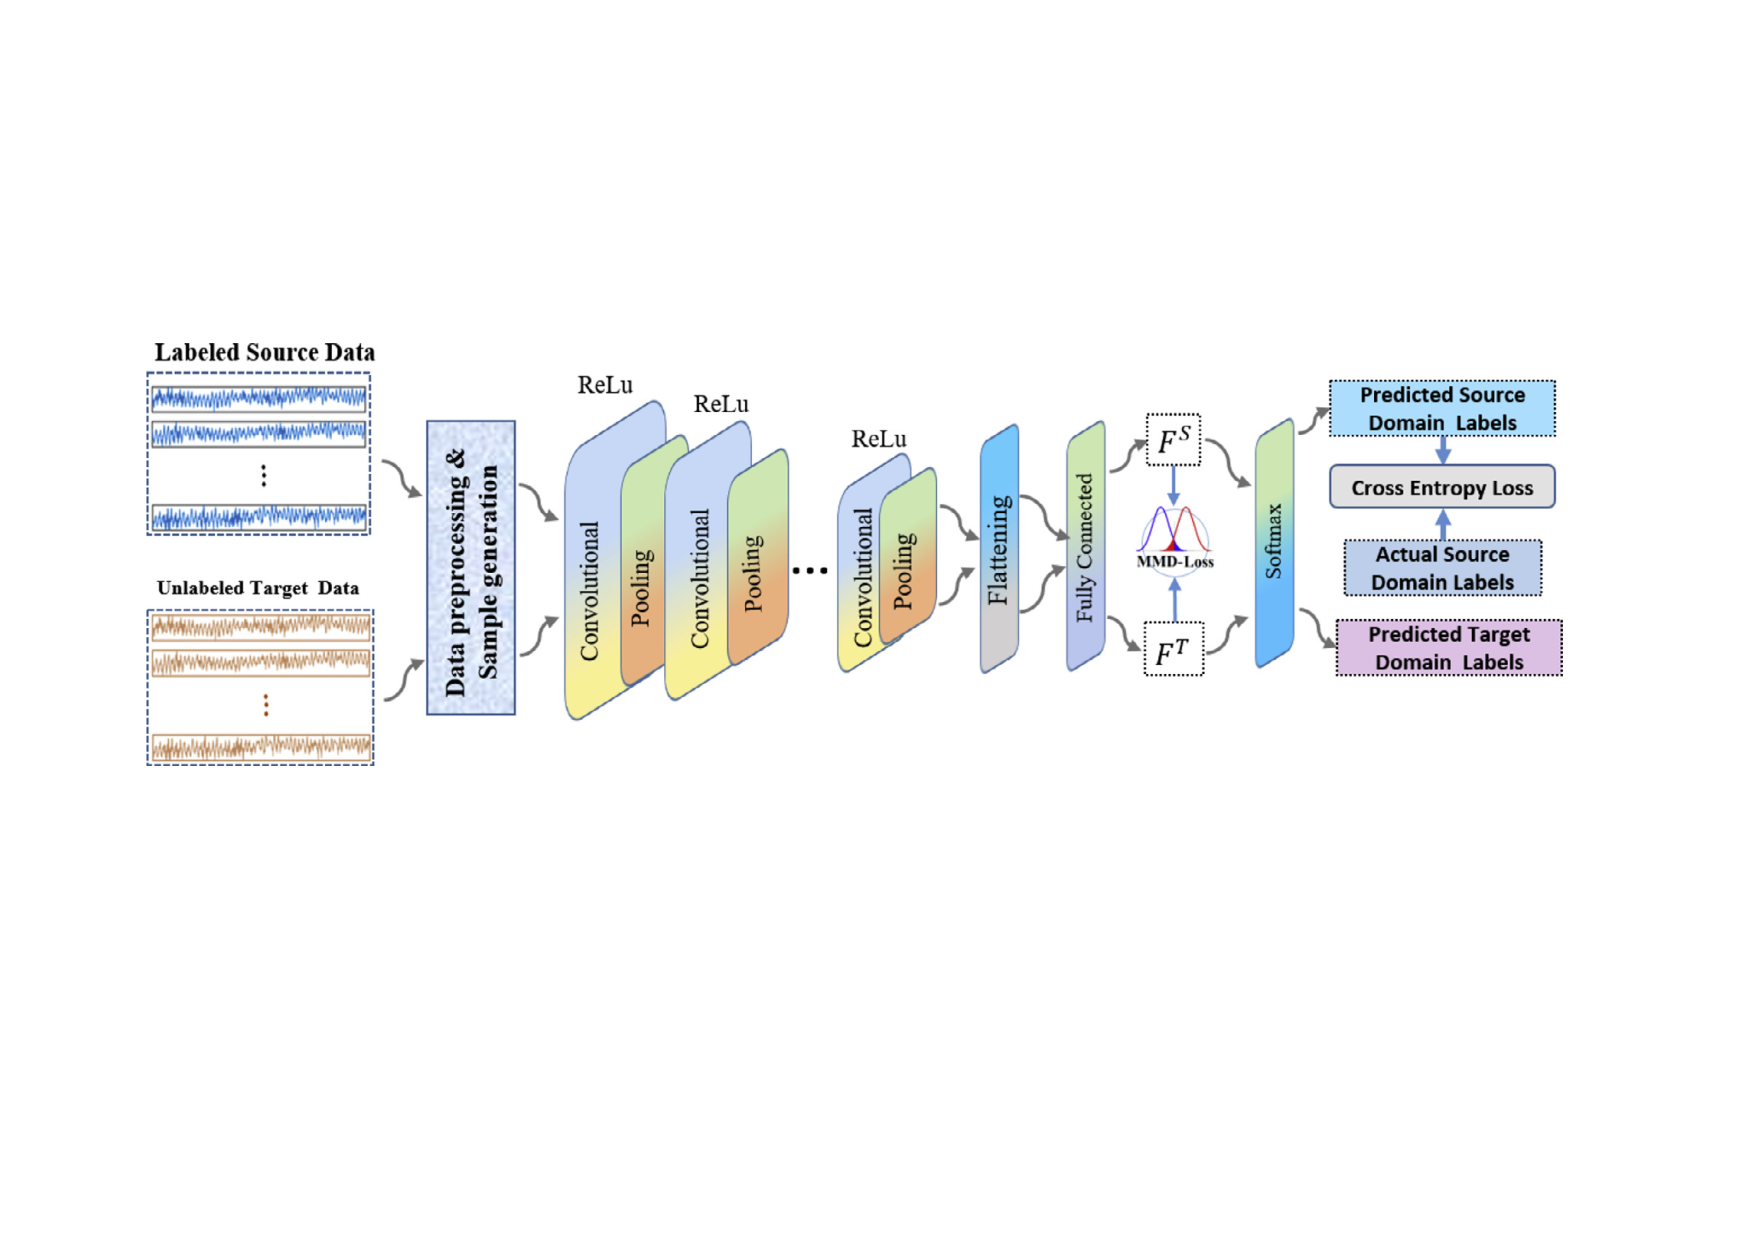
\includegraphics[width=1\textwidth]{models_state_of_the_art/Azamfar_model.pdf}
  \caption{Model architecture of deep learning based domain adaptation model for PHM of BSDs using an MMD-loss \cite{AZAMFAR2020103932}}
  \label{fig:Azamfar_model}
\end{figure}


\subsubsection{Deep Learning Based Domain Adaptation Based on MMD-Loss and PD Alignment}
Similar to Azamfar et al. \cite{AZAMFAR2020103932}, Pandhare et al. \cite{Pandhare2021} proposed a deep learning based domain adaptation model for estimating the health condition of BSDs based on their preload level. A similar test rig, as the one presented by Azamfar et al. \cite{AZAMFAR2020103932}, was used to evaluate the proposed models. In total, five accelerometers were mounted on the testbed. Two triaxial ones were placed close to the BSD nut, which is a promising position to represent the signature of the ball screw preload level. Three single-axial ones were mounted at the bottom and top attachments of the BSD screw shaft and on top of the load carried by the BSD nut. These sensor positions are more suitable and practical installations. Identical to Azamfar et al. \cite{AZAMFAR2020103932}, nine combinations of BSD and guideway preload classes were defined. By using data recorded with sensors mounted at different positions in the BSD testbed, a domain shift between the training and testing dataset was created. Pandhare et al. \cite{Pandhare2021} tried to find an indirect sensing method to make PHM independent of impractical sensor locations. The proposed model architecture is presented in figure \ref{fig:Pandhare_model}. It contained a CNN of two alternating 1D convolutional and max pooling layers and a consecutive classifier. The proposed model training included three losses. Again, a source CE-loss was used to improve the classification performance on the source domain data. An MMD-loss and PD alignment reduced the domain discrepancy between the training and testing dataset. The MMD-loss reduced the marginal and the PD alignment the conditional distribution discrepancy between the domains. The PD alignment matched source and target samples of the same class and reduced their L2-distance: 

\begin{equation}
    L_{p} = \frac{1}{n_{p}}\sum_{k=1}^{n_{p}}|h_{k}^{p,s}-h_{k}^{p,t}|_{2}, 
\end{equation}
where $h_{k}^{p,s}$ and $h_{k}^{p,t}$ are the k-th source and target domain samples and $n_{p}$ is the used subspace of labeled source and target domain samples. The PD alignment was restricted to some of the nine classes and 20\% of the training samples were used as PD samples. The MMD-loss and the PD alignment were restricted to the penultimate fully connected layer \cite{Pandhare2021}.
\begin{figure}[H]
  \centering
  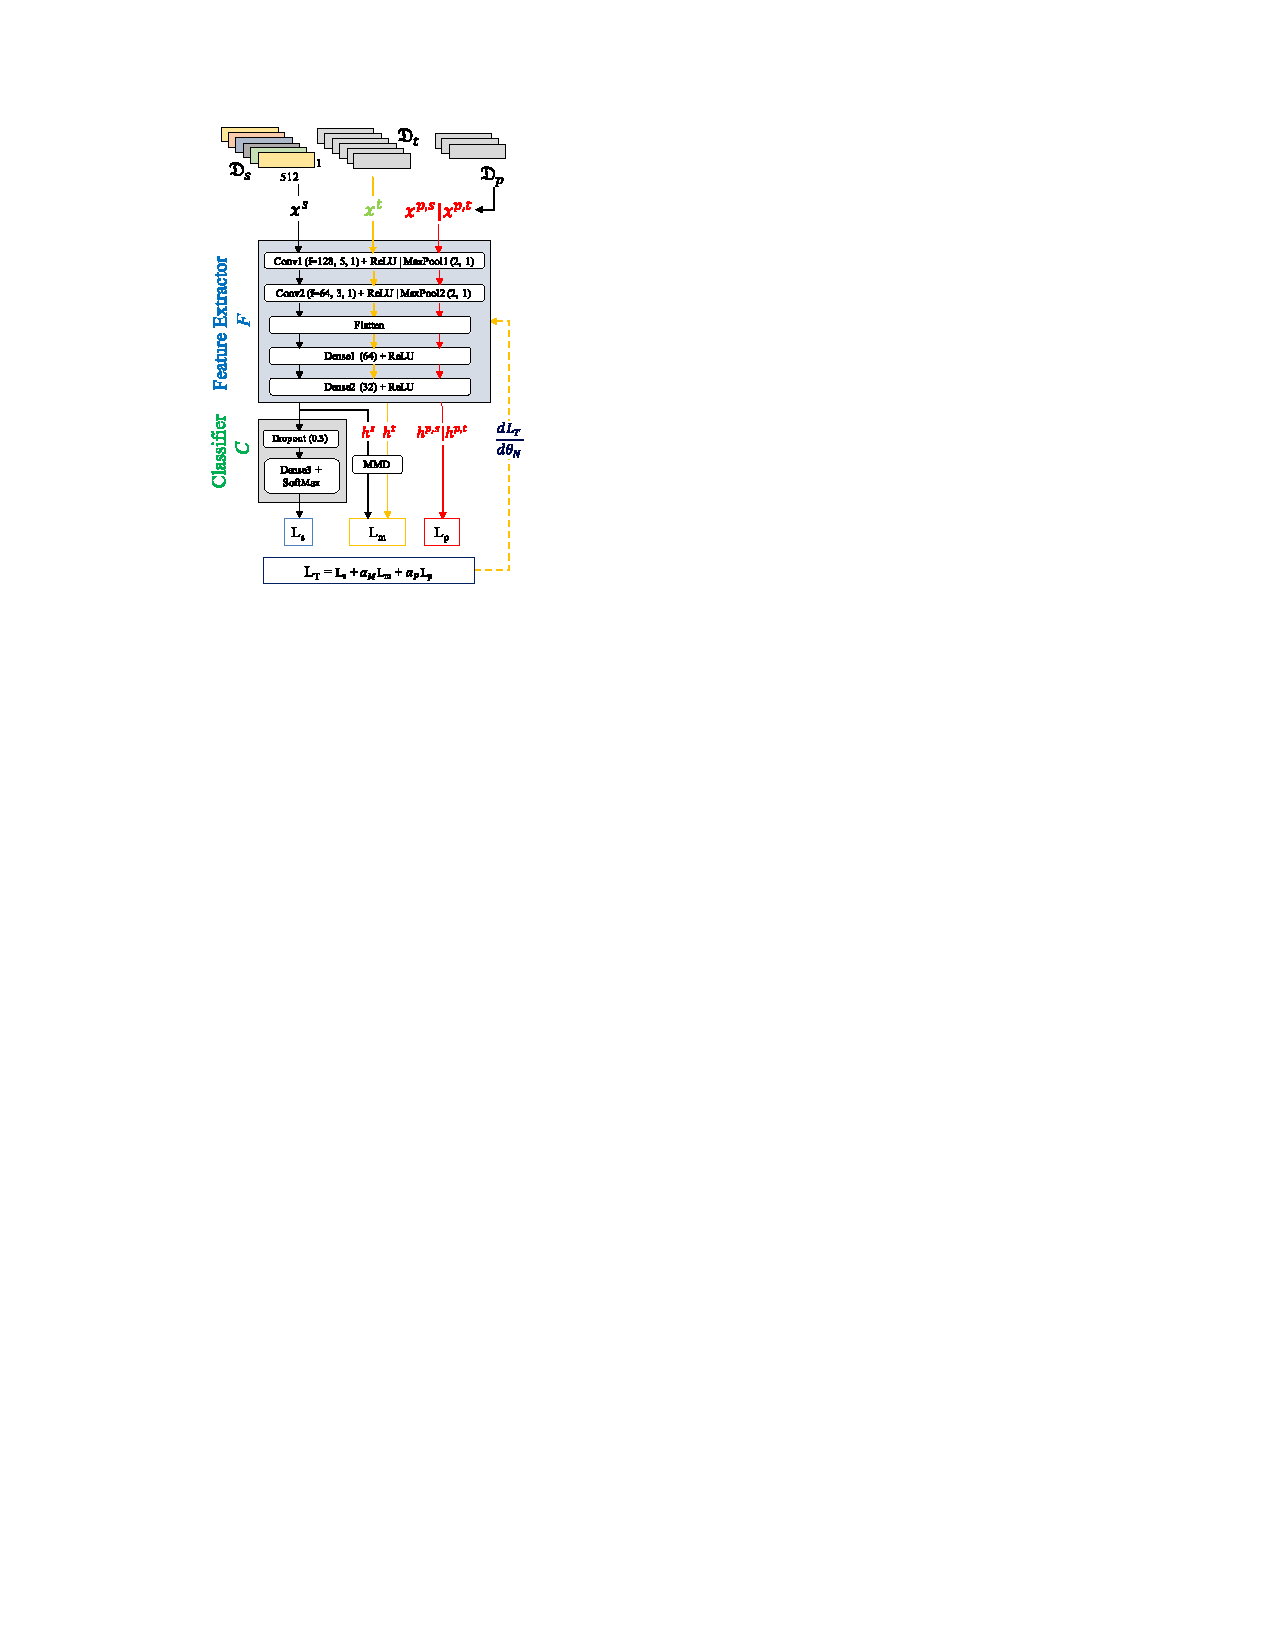
\includegraphics[width=.55\textwidth]{models_state_of_the_art/Pandhare_model.pdf}
  \caption{Model architecture of deep learning based domain adaptation model for PHM of BSDs using an MMD-loss and PD alignment \cite{Pandhare2021}}
  \label{fig:Pandhare_model}
\end{figure}

\subsubsection{Conclusion}
The disadvantages of the presented approaches by Azamfar et al. \cite{AZAMFAR2020103932} and Pandhare et al. \cite{Pandhare2021} are collectively presented in this section. Both approaches applied a regime separation to split the signals into phases of constant and changing BSD velocities \cite{Pandhare2021} \cite{AZAMFAR2020103932} . This extra step adds additional complexity to the data pre-processing. The segments with constant BSD velocity were fed to the models as single samples \cite{Pandhare2021} \cite{AZAMFAR2020103932}. Since those samples capture the frequency and amplitude variations during the whole steady-state phase of the BSD operation, they were assumed to be more expressive for the monitoring task \cite{AZAMFAR2020103932}. By doing so, only a few samples were collected from each recording. Experimental effort was required to record enough samples to train the neural network properly. Azamfar et al. \cite{AZAMFAR2020103932} and Pandhare et al. \cite{Pandhare2021} evaluated their monitoring approaches solely on a simplified testbed. Therefore, the evaluation of their approaches did not consider the mutual influence of the components installed in real-world industrial machines. Additionally, both approaches were restricted to predicting BSD preload forces. Other damages like pitting were ignored by the monitoring systems \cite{Pandhare2021} \cite{AZAMFAR2020103932}. In both cases, the MMD-loss was solely applied in the last fully connected layer. The domain discrepancy reduction was not evaluated in any other latent feature maps of the model \cite{Pandhare2021} \cite{AZAMFAR2020103932}. Azamfar et al. \cite{AZAMFAR2020103932} created a domain shift by recording data with different BSD velocities and Pandhare et al. \cite{Pandhare2021} by recording data with accelerometers mounted at different positions in the BSD testbed. In both cases, the domain shift was not generated by any differences on the physical component level. The same physical components were represented in both domains and therefore, in the training and testing dataset as well \cite{Pandhare2021} \cite{AZAMFAR2020103932}. The PHM systems only had to deal with domain shifts created by variations in the BSD operational conditions and data recording. It was not evaluated how the presented approaches react to physical variations in the systems. The PD alignment approach, presented by Pandhare et al. \cite{Pandhare2021}, requires target labels from some of the considered classes. This simplifies the health condition monitoring task and is rather more impractical for real-world PHM systems.

\subsection{Domain Adaptation Approaches for Prognostic and Health Management of Rolling Bearings}

A PHM system for rolling bearings was presented by Li et al. \cite{Li2018}. In a preprocessing step, a FFT transform was applied to represent the raw vibration signals in the time-frequency domain. As visualized in figure \ref{fig:Deep_distance_metric_learning_model}, the proposed model contained a CNN and a consecutive classifier. Max-pooling layers were included to reduce the model size. Batch-normalization layers reduced the internal covariate shift by normalizing the input distributions of the hidden layers. To prevent overfitting, dropout layers with a rate of 0.5 were included. The proposed method was evaluated on a rolling bearing dataset provided by the Bearing Data Center of Case Western Reserve University. A domain shift was generated by using testing data, which was exposed to additional environmental noise and collected under different working conditions. Ten health conditions with faults in different locations and with varying extents were defined. 

\begin{figure}[H]
  \centering
  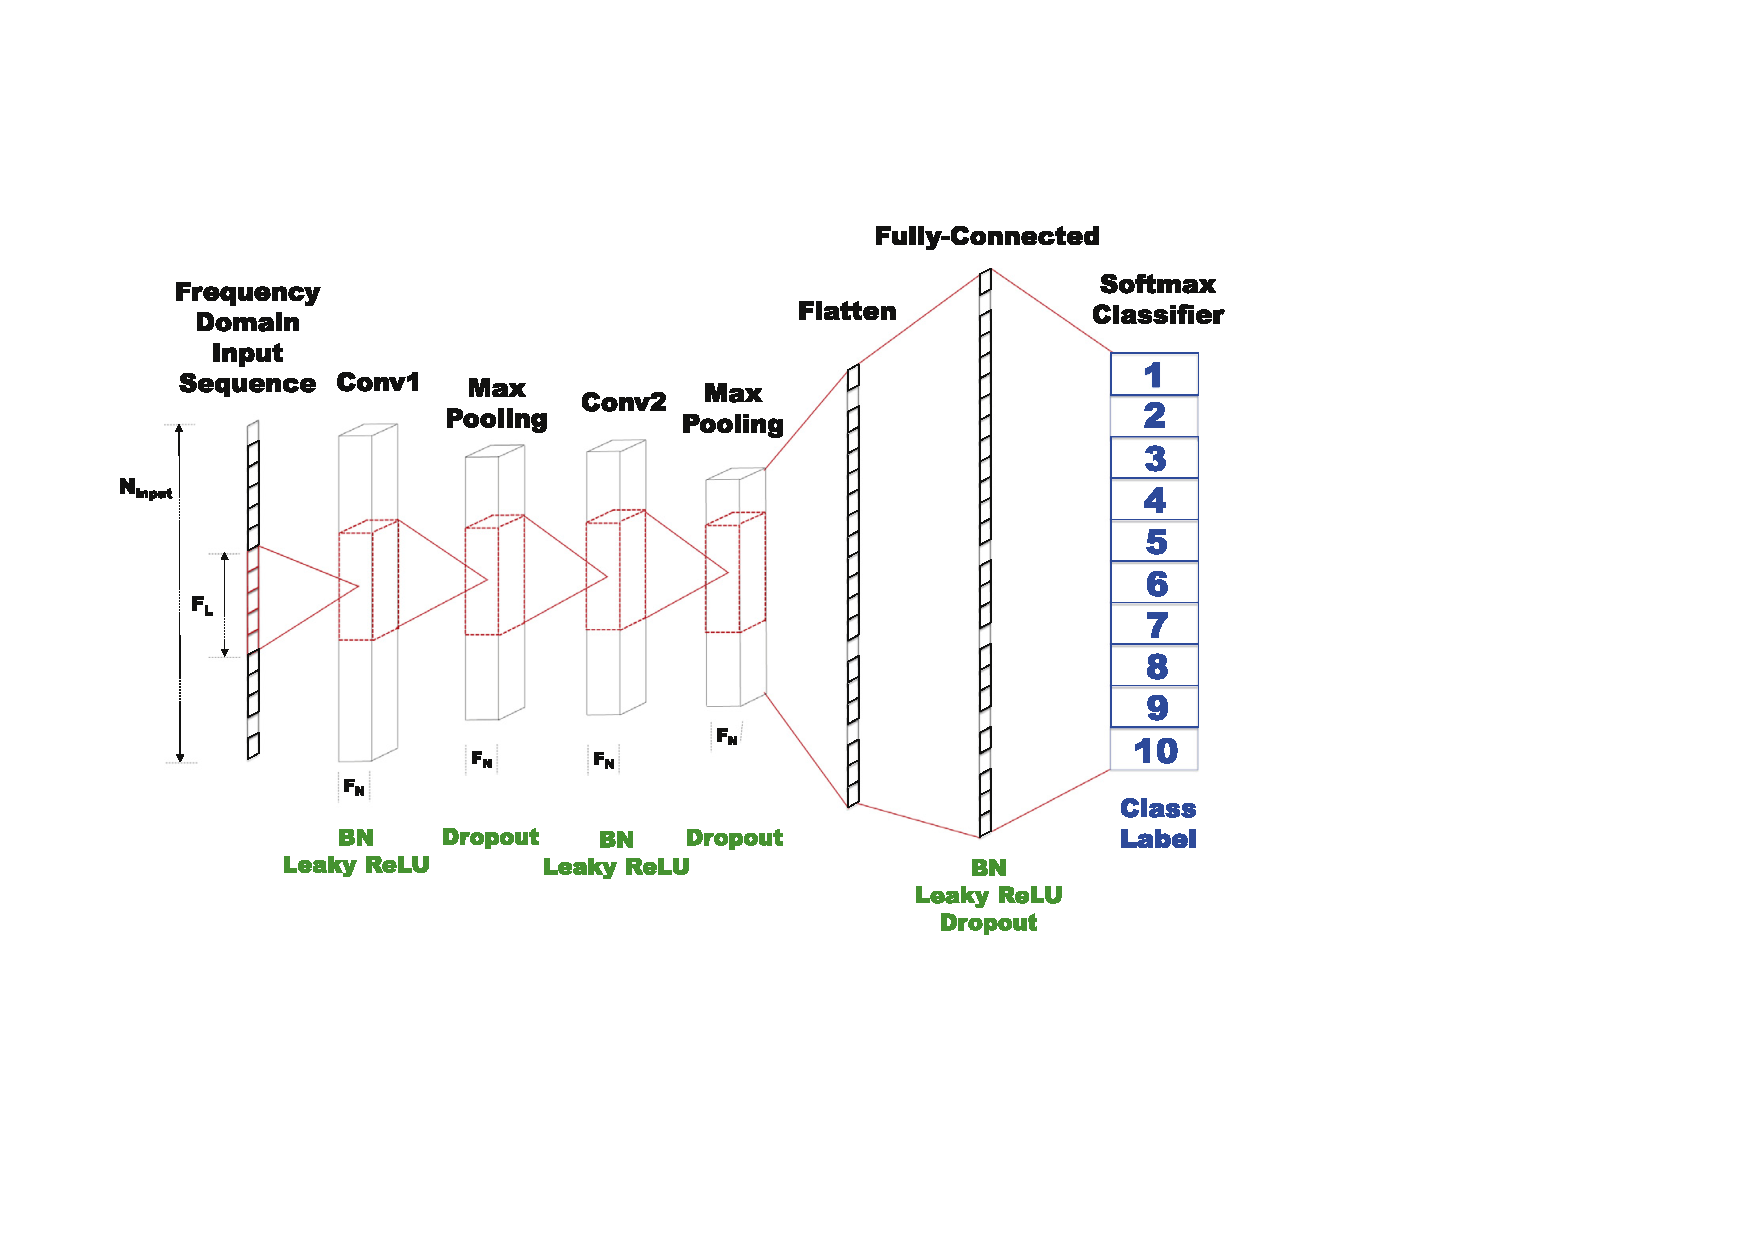
\includegraphics[width=.8\textwidth]{models_state_of_the_art/Deep_distance_metric_learning_model.pdf}
  \caption{Model architecture of deep learning based domain adaptation model for PHM of rolling bearings using an MMD-loss and deep distance metric learning \cite{Li2018}}
  \label{fig:Deep_distance_metric_learning_model}
\end{figure}


The proposed system optimized the inter- and intra-class distance in the latent feature space. The distance between the source samples was minimized if they belonged to the same class and maximized otherwise. This increased the separability and compactness of the source domain classes, which made the algorithm more robust against environmental noise. In order to calculate the intra- and inter-class distances, the expectation and variance of the source domain samples belonging to the same class were measured in the feature maps:

\begin{equation}
    \begin{aligned}
       &D_{inter} = |E[f^{(m)}x^{(i)}]-E[f^{(m)}x^{(j)}]|_{2}-\sqrt{Var[f^{(m)}x^{(i)}]}-\sqrt{Var[f^{(m)}x^{(j)}]}\\
       &D_{intra} = 
        \sum_{i=1}^{N_{class}} \sqrt{Var[x^{(i)}]},
    \end{aligned}
\end{equation}

where $N_{class}$ is the number of classes, $x^{(k)}$ denotes the raw input sample of class k, $f^{(m)}x^{(k)}$ denotes the feature representation of this sample in the m-th layer and $E[f^{(m)}x^{(i)}]$ and $Var[f^{(m)}x^{(i)}]$ are the corresponding expectation and variance. The inter- and intra-class distance were optimized with the following loss: $J_{Cluster} = - D_{inter} + \eta D_{intra}$. In addition to the distance metric learning, the discrepancy between the source and target domain was reduced by an MMD-loss applied in several fully connected (FC) layers. Lastly, the source CE-loss in the final layer optimized the model to classify the source samples correctly. In total, the network was trained with the following weighted average of losses: 

\begin{equation}
    \begin{aligned}
    J_{total} = \alpha J_{Cluster} + \beta J_{MMD} + \gamma J_{CE}, 
    \end{aligned}
\end{equation}
where $J_{Cluster}$ is the loss, optimizing the distances between the source domain samples, $J_{MMD}$ the MMD-loss, $J_{CE}$ the source CE-loss and $\alpha$, $\beta$ and $\gamma$ are the weights for calculating the weighted average \cite{Li2018}.

\subsubsection{Conclusion}
There are several MMD-based domain adaptation approaches for PHM of rolling bearing \cite{AN201942} \cite{Li2018} \cite{Guo2019} \cite{Singh2019} \cite{Kang2020}. Generally, BSDs and rolling bearings are related components. The screw shaft of BSDs can be seen as the inner and the corresponding nut as the outer ring of rolling bearings \cite{Lee2015}. In both cases, balls between those two components allow a rotatory motion around a fixed axis. Other than rolling bearings, BSDs also translate this rotatory motion into a linear one. The degradation of rolling bearings and BSDs is related in some sense. However, PHM systems for rolling bearings cannot be relied on to work as well for BSDs. Still, the research in this domain offers interesting applications and details for the PHM of BSDs. 

Even though the MMD-loss was applied in several layers, it was still restricted to those of the classifier. Furthermore, only noise and different operational conditions created the domain shift but the same physical components were used in the training and testing dataset. Other than the work of Azamfar et al. \cite{AZAMFAR2020103932} and Pandhare et al. \cite{Pandhare2021}, the system was able to monitor different degradation types.

\section{CNN-Based Domain Adaptation in Computer Vision Applications} \label{sec:domain_adaption_CV}

\begin{comment}
\subsection{Domain Conditioned Adaptation Network}
Li et al. \cite{li2020} propose a domain conditioned adaptation network (DCAN), which contains two separate modules to reduce the domain discrepancy. After each task-specific layer a domain conditioned feature correction block estimates and reduces the domain discrepancy based on the MMD metric. In the CNN backbone an attention module regulates the extraction of domain-specific and -independent features. The proportions of domain-specific and -independent features is learned to decrease the domain discrepancy. Fig. \ref{fig:DCAN_model} visualizes the domain adaptation modules in the DCAN model.

\subsubsection{Domain Conditioned Channel Attention Mechanism}
ResNet is used as a backbone network, which allows an easy implementation of the domain conditioned channel attention module in its residual block. In the latent feature maps, the processed images are represented as $\pmb{X}_{t} = [X^{1}_{t},...,X^{C}_{t}] \in \mathbb{R}^{HxWxC}$, where H and W are the spatial dimension and C the number of image channels. First, a channel-wise global average pooling layer is applied, which reduces the images to  $\pmb{g}_{t} = [g^{1}_{t},...,g^{C}_{t}] \in \mathbb{R}^{1x1xC}$. Afterwards, the data is split depending on its domain and passed through different fully connected layers. The upper flow is used for target and the lower flow for source domain samples. The two different source and target domain routes share parameters. For both domains, an attention mechanism is trained jointly to learn activating different channels in the domain samples. This allows extracting more enriched domain-specific features. In the fully connected layers the dimension is first reduced with a ratio ${1x1x\frac{C}{r}}$ and later reconstructed to its original size ${1x1xC}$. ReLU and Sigmoid functions are applied. The domain-wise feature selection is achieved by weighting the channels of the feature representations $\pmb{X}_{s}$ and $\pmb{X}_{t}$ with the channel attention vectors $\pmb{v}_{s}$ and $\pmb{v}_{t}$ calculated by the domain conditioned channel attention module:

\begin{equation}
    \begin{aligned}
        &\pmb{\tilde{X}}_{s} = \pmb{v}_{s} \odot \pmb{X}_{s} = [v_{s}^{1} \cdot X_{s}^{1}, ..., v_{s}^{C} \cdot X_{s}^{C}]\\
        &\pmb{\tilde{X}}_{t} = \pmb{v}_{t} \odot \pmb{X}_{t} = [v_{t}^{1} \cdot X_{t}^{1}, ..., v_{t}^{C} \cdot X_{t}^{C}].
    \end{aligned}
\end{equation}

The domain conditioned channel attention module allows the model to independently learn the importance of each channel for the classification of source and target domain samples \cite{li2020}.

\subsubsection{Domain Conditioned Feature Correction}
The data simultaneously passes through the regular network and the feature correction block, which consist of FC and ReLU blocks. The feature correction block estimates the domain discrepancy in the feature representation of the task-specific layer:
\begin{equation}
    \Delta H_{l}(x_{t}) = H_{l}(x_{s}) - H_{l}(x_{t}),
\end{equation}
where $H_{l}(x_{s})$ and $H_{l}(x_{t})$ are the feature representations of the source and target domain samples in the task-specific layer l. $\pmb{x}_{s}$ and $\pmb{x}_{t}$ are the source and target domain samples. The feature representation of the target domain samples is corrected as following:

\begin{equation}
    \hat{H}_{l}(x_{t}) = H_{l}(x_{t}) + \Delta H_{l}(x_{t}).
\end{equation}

The discrepancy between the regular feature representation of source domain samples $H_{l}(x_{s})$ and the corrected feature representation of the target domain samples $\hat{H}_{l}(x_{t})$ is measured by the MMD-loss in several layers:

\begin{equation}
    L_{M}^{l} = |\frac{1}{n_s} \sum_{i=1}^{n_{s}} \phi(H_{l}(x_{si}) - \frac{1}{n_t} \sum_{i=1}^{n_{t}} \phi(\hat{H}_{l}(x_{ti}))|_{H_{\kappa}}^{2}, 
\end{equation}
where $H_{\kappa}$ is the reproducing kernel Hilbert space (RKHS), $\kappa$ the characteristic kernel and $\phi$ the corresponding feature map. The number of source and target samples is defined by $n_{s}$ and $n_{t}$. To avoid the over-transfer of noise and irrelevant information between source and target, the model is enforced to keep the source data constant when passing through the feature correction blocks \cite{li2020}.

\begin{figure}[H]
  \centering
  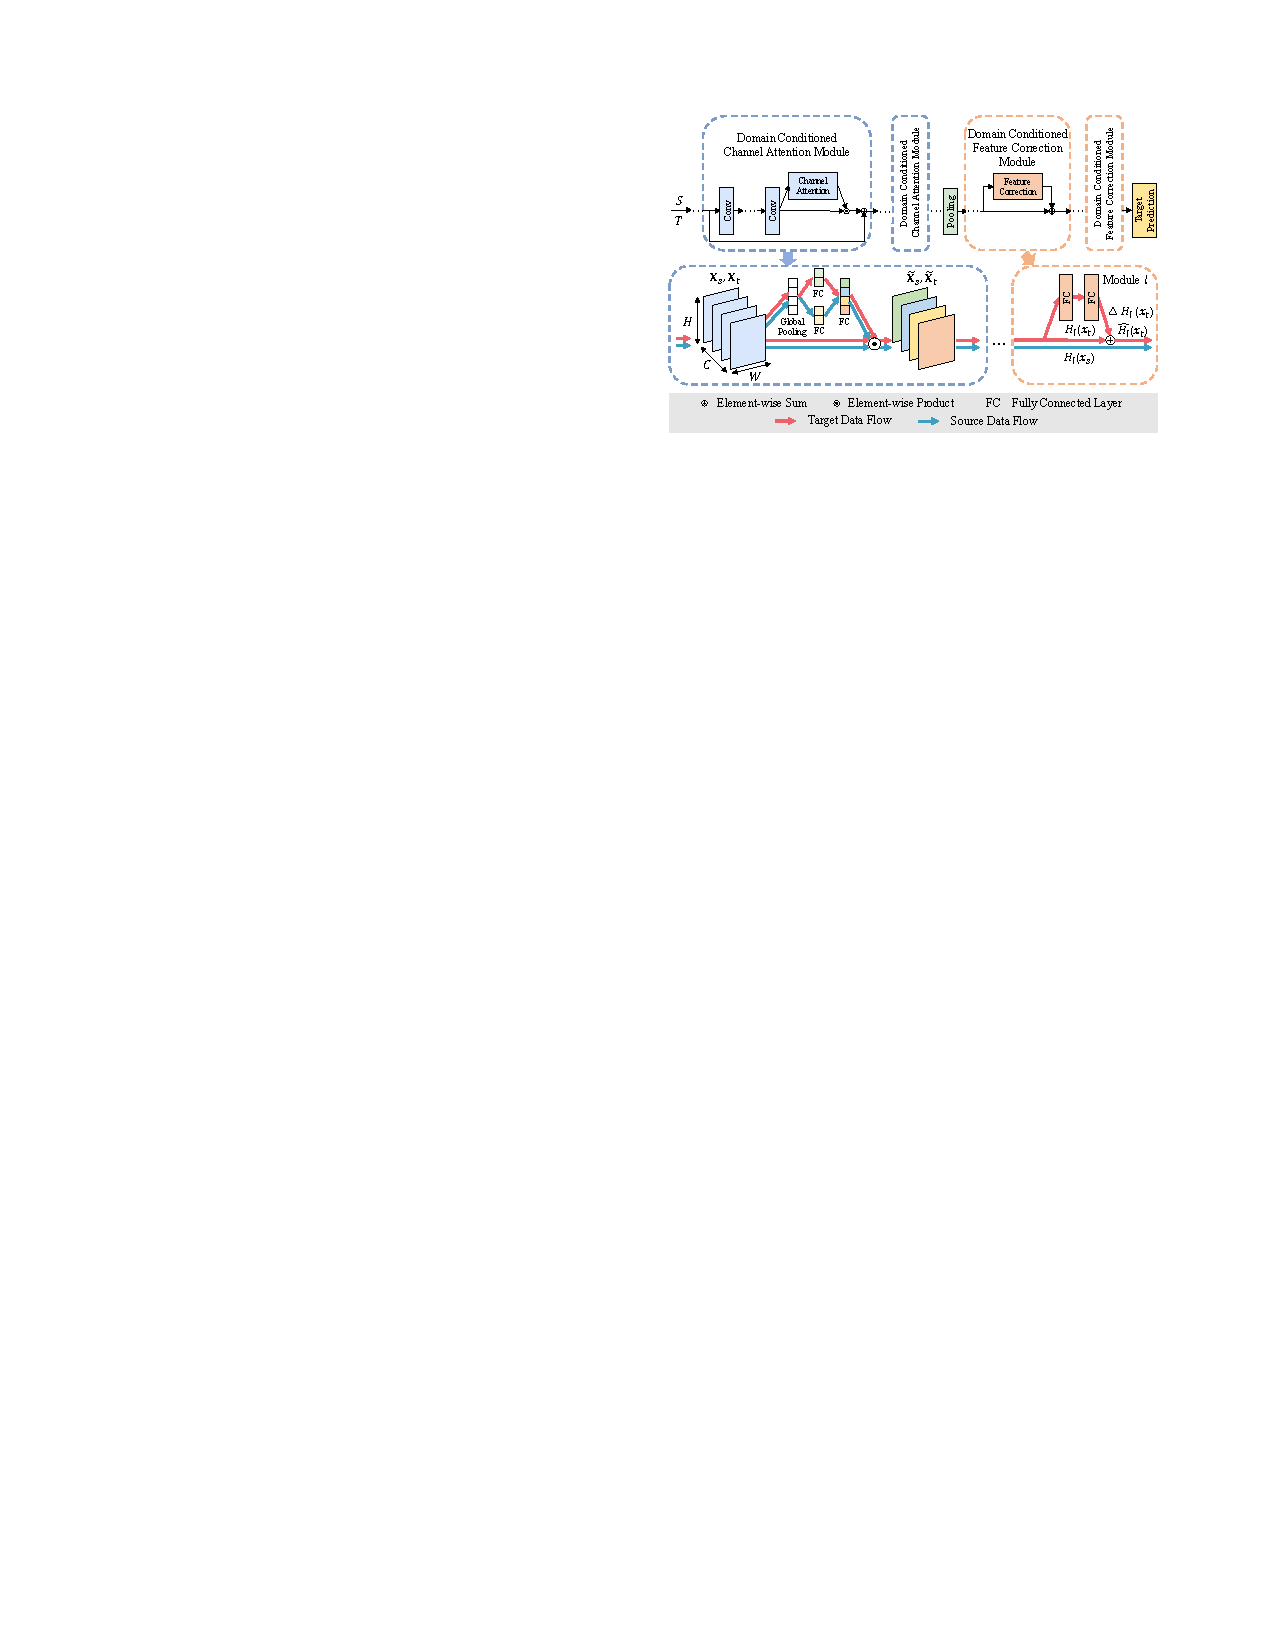
\includegraphics[width=1\textwidth]{models_state_of_the_art/DCAN_model.pdf}
  \caption{DCAN architecture proposed by Li et al. \cite{li2020}}
  \label{fig:DCAN_model}
\end{figure}

\end{comment}

%\subsection{Feature Reconstruction of Domain Shift Affected Layers}
Aljundi et al. \cite{Aljundi2016} presented a domain adaptation approach for computer vision applications. The method analyzed the domain shift effects in all convolutional layers of the neural network. Strongly affected feature maps (bad filters) were identified and reconstructed by less affected ones (good filters). Additionally, the domain discrepancy of the feature maps was measured by the Kullback-Leibler (KL) divergence. The feature maps' influence during the reconstruction process was punished accordingly. During the optimization, one filter map was considered at a time. In each filter map evaluation, those feature maps should be identified which were able to reconstruct the response of the evaluated one:
\begin{equation}
    B^{*} = argmin_{B} \{ \sum_{i=1}^{n}( y_{i}-\beta_{0}-\sum_{j=1}^{p}x_{i,j}\beta_{j})^{2} + \lambda \sum_{j=1}^{p}|\Delta_{j}^{KL}\cdot \beta_{j}| \},
\end{equation}
where $y_{i}$ is the output of the evaluated filter map for the sample $i$, $x_{i,j}$ the output of the feature map $j$ for the sample $i$, $\beta_{0}$ the residual, $B = \{\beta_{j}\}$ the coefficients, estimating the suitability of each feature map to reconstruct the output of the evaluated feature map, $n$ the number of source samples, $p$ the number of layers, $\lambda$ a tuning parameter to punish the coefficients and $\Delta_{j}^{KL}$ the KL divergence measured between the source and target data representations in layer $j$. When a layer's coefficient  $\beta_{j}$ was big, it was considered as good (small domain shift effects) and otherwise as bad (big domain shift effects). The optimization was solved by using the coordinate descent method. Afterwards, linear regression was applied to reconstruct the output of the bad layers by a weighted average of the good ones. The reconstructed layer outputs were then passed to the subsequent layers. Aljundi et al. \cite{Aljundi2016} identified the CNN's early layers to be especially relevant to counteract the domain shift. In this context Aljundi et al. \cite{Aljundi2016} also gave a great hypothetical example of how early layers of CNNs can generate domain shifts. If one imagines a neural network for recognizing facial expressions, early layers of the CNN usually detect things like colors and edges. When training such a model with young faces and testing it with those of old people, the model is confronted with wrinkles, which it has not seen during training. These wrinkles could distract the system to recognize those edges, which are relevant for identifying facial expressions. By adapting those early layers, which are responsible for edge detection, to be less prone to wrinkles, the domain shift could be reduced efficiently \cite{Aljundi2016}. 

\subsubsection{Conclusion}
The presented approach by Aljundi et al. \cite{Aljundi2016} disagrees with most domain adaptation approaches, which reduce the domain discrepancy in task-specific layers but use a shared CNN backbone across all domains. The work shows the positive effect of reducing the domain shift in the early layers of the CNN \cite{Aljundi2016}. There is no clear pattern of which layers contribute most to the domain discrepancy problem \cite{Aljundi2016}. Therefore, it is a great approach to evaluate each layer individually and adapt them adequately to reduce the domain shift. The work shows, that early layers in the CNN already suffer from and contribute to the domain shift \cite{Aljundi2016}. Often the computer vision community offers advanced solutions for complex research questions which were not intensively evaluated in real-world scenarios. For the PHM of BSDs such solutions can be taken as inspiration.

\section{Research Gap}\label{ch:research_gap}
When industrial machines run over long periods of time, varying operational conditions change the fault characteristics in the machine data \cite{AZAMFAR2020103932}. Due to the mutual influence of the machine's submodules, fault characteristics are often complex and highly dependent. Developing hand-crafted features, as they are quite common in traditional approaches, requires a lot of expertise and human labor \cite{ZHAO2019213}. Due to the lack of flexibility and robustness, hand-crafted features struggle to extract expressive information from the machine data when the corresponding fault characteristics vary over time \cite{ZHAO2019213}.
Model-based PHM systems, like those presented by Lee et al. \cite{Lee2015} and Nguyen et al. \cite{NGUYEN2019}, predict the BSD's health condition based on simplified physical models. The quality of those approaches highly depends on the exactness and sophistication of the underlying models and the corresponding parameters. If the models miss details from the real-world machines or the underlying processes, the PHM performance will be unsatisfactory \cite{ZHAO2019213}.
Data-driven PHM systems, like those proposed by Denkena et al. \cite{Denkena2021} and Li et al. \cite{LiPin2018}, use shallow machine learning classifiers in the final steps of the processing chain. These classifiers learn to use the information extracted by the hand-crafted features to make accurate predictions \cite{ZHAO2019213}. This intelligent way of combining the knowledge retrieved by the hand-crafted features might make those systems less prone to minor variations in the fault characteristics. Since the classifiers automatically learn the correlation between the hand-crafted features and the health condition classes, adapting such systems to new circumstances could be less time-consuming. Nevertheless, the system's performance highly depends on the underlying training dataset. It is unlikely that the training data includes all operational conditions and fault scenarios. It can even happen that fault classes are unknown during training. Optimizing machine learning models with limited data, which does not represent the data distributions during testing, could lead to a low diagnosis performance \cite{AZAMFAR2020103932}.

Robust PHM systems, designed to reliably handle fault characteristic variations, will bring industrial health monitoring to the next level \cite{Michau2017}. In order to achieve that, PHM systems can be extended with domain adaptation modules. This thesis should investigate the applicability and utility of deep learning based domain adaptation for health condition monitoring of BSDs. The advantages of the proposed system over regular deep learning based systems should be evaluated. It requires a lot of work to establish accurate physical models and expressive hand-crafted features, which capture the degradation of BSDs \cite{ZHAO2019213}. For this reason, it is difficult to compare the developed approach to any traditional model-based or data-driven PHM system.

Most MMD-based domain adaptation systems for PHM tasks \cite{Pandhare2021} \cite{AZAMFAR2020103932} \cite{Li2018}, apply the MMD-loss solely in task-specific layers. In the PHM context, the literature rarely discusses variations in this application of the MMD-loss. Inspired by the advances in the computer vision community \cite{li2020} \cite{Aljundi2016}, this thesis should evaluate different MMD-loss types and corresponding hyperparameters for monitoring the health condition of BSDs.

All presented approaches in chapter \ref{chapter:related_works} were evaluated on a simplified testbed. In most of the experiments executed in this process, the degradation of the monitored components was just simulated and not caused by field use. The traditional PHM approaches presented in chapter \ref{sec:traditional_approaches} did not consider varying degradation levels of LGSs while predicting the health condition status of BSDs. Pandhare et al. \cite{Pandhare2021}, Azamfar et al. \cite{AZAMFAR2020103932} and Li et al. \cite{Li2018} created a domain shift by recording data with different sensors of by retrieving data from varying operational conditions of the machine. However, in the training and testing dataset the same physical components were represented. Furthermore, the models developed by Pandhare et al. \cite{Pandhare2021} and Azamfar et al. \cite{AZAMFAR2020103932} solely monitored the preload level of BSDs.

Since the lifetime of BSDs is shorter than that of LGSs, in industrial machines, the BSDs need to be replaced in shorter intervals than the LGSs. Thus, it is very common that BSDs and LGSs with different levels of degradation are combined in industrial machines \cite{Li2018}. This implies that the developed model in this thesis should be able to predict the health condition classes of BSDs independent of the degradation of LGSs. In real-world PHM tasks, only a limited number of observations of all health condition classes are available during training. Typically, the physical components available during training differ from those during testing. Therefore, a PHM system should be developed that is robust enough to predict the health condition of new and unseen components during testing. Additionally, it should investigated how a PHM system can learn to monitor different degradation types simultaneously. A strong domain shift should be included in the dataset to generate a challenging PHM task. The developed model should be evaluated on a real-world machine with BSDs and LGSs degraded by field use. 







\chapter{Research Questions}\label{chapter:research_approach}
The thesis is centered around three main research questions, which are presented in the following. In the end of this chapter the approach to investigate those three questions is explained. These questions were defined beforehand to ensure that the developed PHM systems are analyzed properly. The questions were formulated based on common problems and challenges in the domain adaptation and PHM community. 

\section{Influence of Latent Feature Space Choice on the Domain Adaptation Performance}
Most domain adaptation approaches, just as the one presented by Azamfar et al. \cite{AZAMFAR2020103932} and Pandhare et al. \cite{Pandhare2021}, reduce the domain discrepancy in the task-specific layers but use a shared feature extractor backbone across all domains. Throughout the neural network, the feature maps contain information with different levels of abstraction. In shallow layers, more global and in deeper layers more task-specific features are extracted \cite{Aljundi2016}. Often, it is assumed that early convolutional layers extract general information and act as simple detector for things like colour or texture. As the earlier mentioned hypothetical example by Aljundi et al. \cite{Aljundi2016} shows, the influence of those layers on the emerging domain discrepancy throughout the neural network is often underestimated. Li et al. \cite{li2020} assumed that reducing the domain discrepancy just in task-specific layers might minimize but not fundamentally eliminate it. Therefore, Li et al. \cite{li2020} proposed a model which separately learned to extract domain-dependent and -independent features in the convolutional layers to reduce the domain shift. The work of Aljundi et al. \cite{Aljundi2016} shows that layers of the feature extractor are responsible for specific characteristics in deeper latent feature map representations and thus the creation of a dataset bias. Since feature maps influence all subsequent ones, propagating the biased data through the neural network facilitates the domain shift. This shows the significant contribution of the feature extractor layers to the increasing domain shift throughout the neural network. Aljundi et al. suggested the evaluation of the domain shift in convolutional layers and the reconstruction of those which are strongly affected \cite{Aljundi2016}. Inspired by the work of Azamfar et al. \cite{Aljundi2016}, this thesis investigates how applying the MMD loss in the feature extractor can improve the domain discrepancy reduction.


\section{Influence of GAMMA choice on the domain adaptation performance}
Since the source and target domains are correlated to some extent, the network itself can extract domain-independent features. The powerful feature extractor learned from the source domain can also increase the model performance on the target domain. At the same time, features that are too sensitive to the source domain can reduce the model performance on the target domain \cite{li2020}. To counteract that phenomenon, domain adaptation approaches can help to transfer knowledge learned from the source to the target domain. Nevertheless, one has to pay attention to not transfer noise or irrelevant information, since this destroys the structure of the source and target domain data and makes the classification task even more difficult \cite{li2020}. It is important to balance the MMD- and CE-loss very sensible. In this thesis, the effects of different GAMMA choices are investigated.

\section{Domain Adaptation Performance when Using a Labeled MMD-Loss}
In addition to the MMD-based domain reduction, Pandhare et al. \cite{Pandhare2021} applied a PD-alignment module, which specifically reduced the L2-distance between samples belonging to the same class but different domains. The PD-alignment required target labels. Li et al. \cite{Li2018} presented a PHM algorithm, which optimized the source domain inter- and intra-class distance while reducing the domain discrepancy with an MMD-loss. The expectation and variance of source domain samples belonging to the same class were used for the distance-based optimization. The goal of both approaches was to improve the compactness and separability of the class representations, which increases the domain overlap in the latent feature space. A stronger domain similarity facilitates the extraction of domain invariant features. Inspired by those two approaches, this thesis develops a novel labeled MMD-loss, which uses target labels to improve the domain adaptation capabilities of the system. Instead of applying a PD-alignment in addition to an MMD-loss, this novel MMD-loss directly considers the labels of the source and target domain. Like in the work of Pandhare et al. \cite{Pandhare2021}, the target labels are not used in the CE-loss.

\section{Approach}
In the course of this thesis, the performance gain in PHM systems due to domain adaptation approaches is evaluated. The proposed approaches are pre-evaluated on the dummy dataset and afterward extensively tested on a real-world dataset. Experiments on the mentioned datasets are performed for the following reasons:
\begin{itemize}
    \item Evaluation of the applicability of MMD-based domain adaptation for industrial health monitoring
    \item Analysis of the effects of MMD-based domain discrepancy reduction on the data-level
    \item Investigation of the three research questions in the context of BSD health monitoring.
\end{itemize}

The datasets, the proposed model architecture and the corresponding training strategy are presented in chapter \ref{chapter:experiments}. The results from the experiments can be found in chapter \ref{chapter:results}. 
\begin{comment}
\section{Signals used for PHM}
In the work of Pandhare et al. \cite{Pandhare2021} just vibration signals in different spatial directions are measured with sensors, installed at various locations on the BSD. Azamfar et al. \cite{AZAMFAR2020103932} additionally use sound pressure sensors to capture the acoustic level and extract torque and speed signals from the controller. In this thesis also the mechanical power, target electrical power and actual electrical power signals were extracted from the controller. Pandhare et al. and Azamfar et al. record machine data during BSD steady-state motion. In this thesis machine data is collected during different machine excitements (constant speed excitements, direction change excitements and sweep excitement) along the machine tools X-axis. These different signals were evaluated for their suitability for PHM of BSDs


Both Pandhare et al. \cite{Pandhare2021} and Azamfar et al. \cite{AZAMFAR2020103932} feed the data recorded during BSD steady-state motion as one single input to their models. During the phases of constant BSD motion, the amplitude of the signals changess. Azamfar et al. assume that the shorter sequences created by a windowing function just capture limited information about these changes and are therefore not a proper tool for PHM \cite{AZAMFAR2020103932}. In the thesis a windowing function was evaluated for the PHM of BSDs. Windowing functions make the BSD experiments less dependent from specific BSD excitements. When beeing able to check the BSD degradation with short recorded windows, one can make statements about the BSD health status with data redcorded in real time use. Extra experiments 
\end{comment}



\chapter{Experiments and Methods}\label{sec:experiments}
In the chapters \ref{sec:dummy_dataset} and \ref{sec:real_world_dataset} the synthetically generated dummy and real-world BSD datasets are presented. In the course of that, the generation of the datasets, the included domain shift problem and the resulting classification task are described. In the chapters \ref{sec:model} and \ref{sec:methods}, the proposed model architecture, as well as the corresponding training, are presented. 
\section{Dummy Dataset}\label{sec:dummy_dataset}
In the first step, different MMD-based domain adaptation approaches for PHM applications were evaluated on a synthetically generated dummy dataset. Such datasets are structured equally and show similar patterns as the corresponding real-world datasets. The complexity in such datasets and therefore the difficulty of the corresponding tasks can be tuned arbitrarily. When analyzing new and unknown methods, dummy datasets help to understand their underlying mechanisms and effects on the data level. Besides that, dummy datasets pre-evaluate the applicability of such methods for the corresponding real-world task. In this thesis, a simple dummy dataset with a domain shift was created to investigate the ability of MMD-losses to facilitate the extraction of domain-invariant features in neural networks. Since one has to deal with irregularities, outliers and noise in real-world data, it is helpful to evaluate the MMD-loss on a dataset, which is not disturbed by these effects. Similarly to PHM applications, the dummy dataset contained one-dimensional time sequences, each containing 1000 data points. In order to simulate a classification problem with two classes and two domains, the data points of each sequence were sampled from four cosine curves with characteristic amplitudes and frequencies. By adjusting the amplitude and frequency, the domain adaptation problem can be configured more or less difficult. The sampling process included certain randomness to allow variations between sequences of the same class and domain. For every sampled sequence, the characteristic amplitude and frequency of the cosine curve were perturbed. This changed the underlying characteristic of each sequence. Besides that, noise was added to each of the 1000 data points. This is necessary to generate sequences similar to noisy real-world vibration signals. Exemplary samples for both classes and domains are shown in fig. \ref{fig:samples_domain_class_dummy}.

\begin{figure}[H]
  \centering
  \includegraphics[width=.45\textwidth]{samples_domain_class_dummy/Source_Domain_Class_0_obs_0.pdf}
  \hspace{.3cm}
  \includegraphics[width=.45\textwidth]{samples_domain_class_dummy/Source_Domain_Class_1_obs_0.pdf}

  \vspace{.3cm}

  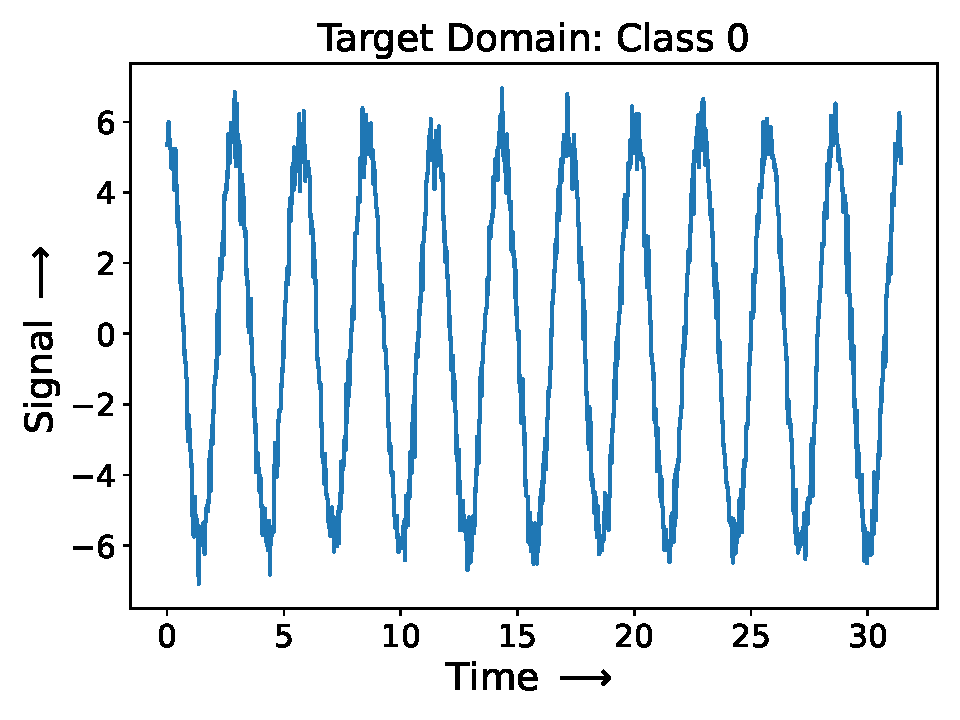
\includegraphics[width=.45\textwidth]{samples_domain_class_dummy/Target_Domain_Class_0_obs_0.pdf}
  \hspace{.3cm}
  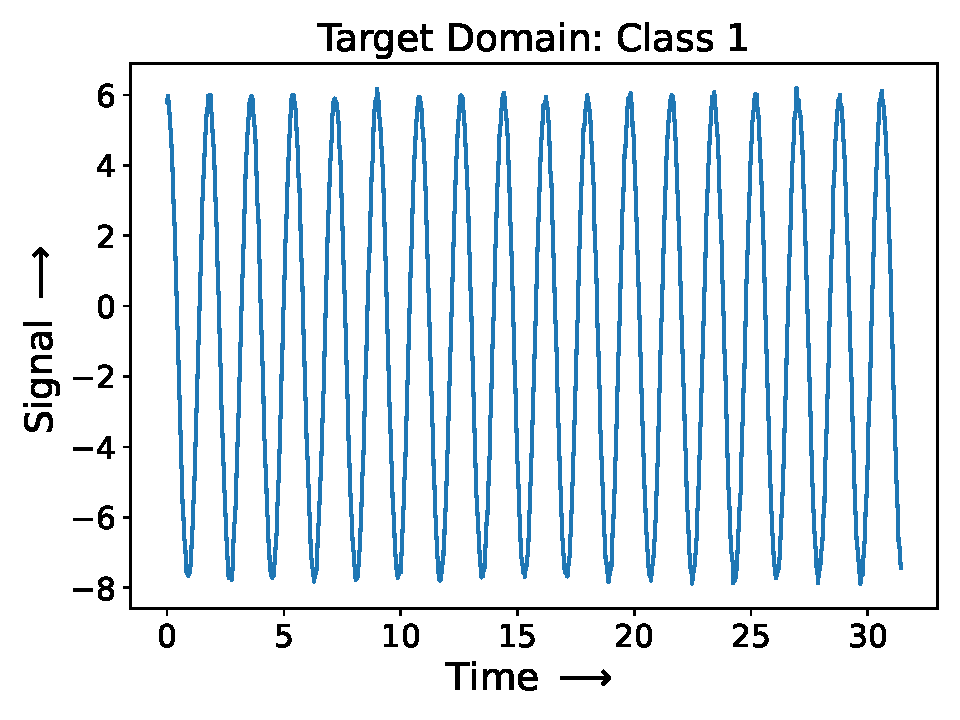
\includegraphics[width=.45\textwidth]{samples_domain_class_dummy/Target_Domain_Class_1_obs_0.pdf}

  \caption{Dummy data samples for the two classes and domains}
  \label{fig:samples_domain_class_dummy}
\end{figure}

Fig. \ref{fig:samples_domain_class_dummy_influence_noise} visualizes how the perturbation of the frequencies and amplitudes, as well as the noise added to each data point, generate quite some differences between sequences of the same class and domain.

\begin{figure}[H]
  \centering
  \includegraphics[width=.45\textwidth]{samples_domain_class_dummy_influence_noise/Source_Domain_Class_0_obs_0.pdf}
  \hspace{.3cm}
  \includegraphics[width=.45\textwidth]{samples_domain_class_dummy_influence_noise/Source_Domain_Class_1_obs_0.pdf}

  \vspace{.3cm}

  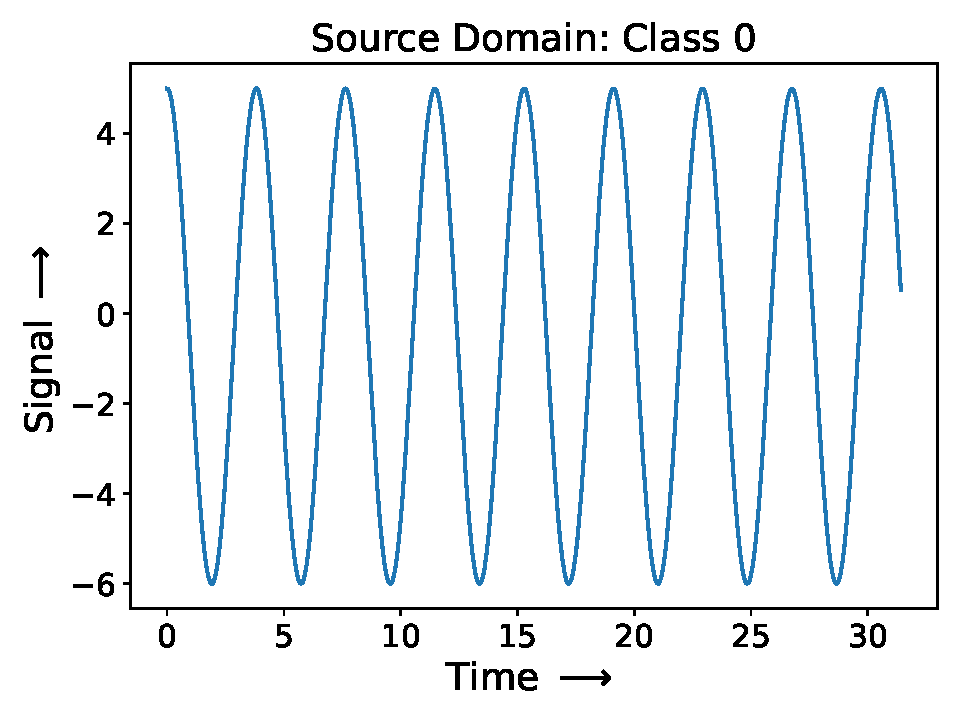
\includegraphics[width=.45\textwidth]{samples_domain_class_dummy_influence_noise/Source_Domain_Class_0_obs_1.pdf}
  \hspace{.3cm}
  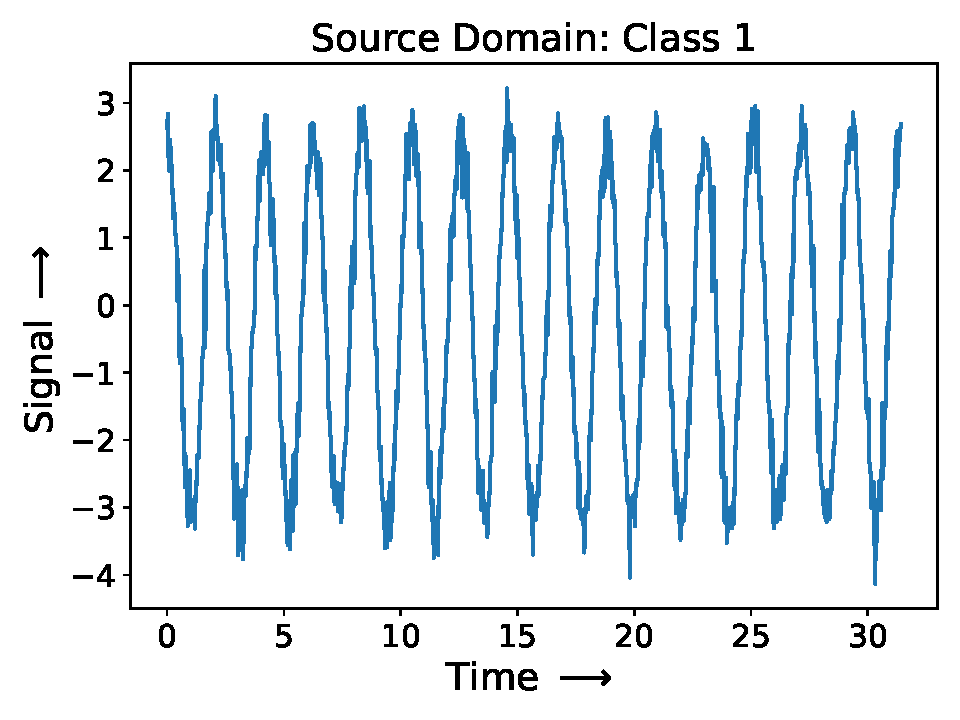
\includegraphics[width=.45\textwidth]{samples_domain_class_dummy_influence_noise/Source_Domain_Class_1_obs_1.pdf}

  \caption{Discrepancy between source samples of equal classes due to applied perturbation and noise in the sampling process}
  \label{fig:samples_domain_class_dummy_influence_noise}
\end{figure}

\section{Dataset: Ball Screw Drive} \label{sec:real_world_dataset}
Testing the developed PHM methods on a real-world dataset is essential to make statements about the method's utility and applicability for industrial PHM tasks. Milling machines are common in the industry and contain several BSDs, which suffer from degradation. The continuous evaluation of the BSD health condition is therefore essential. For this reason, the developed models were applied to a dataset recorded on an industrial milling machine. Their performance was evaluated on the PHM of the corresponding BSDs. In the following, the experimental setup including a description of the mounted sensors, the classification task, the generated domain shift problem, the data recording procedure and the resulting PHM task are presented. 

\subsection{Experimental Setup}
Data from a DMG DMC 55H duoblock milling machine of the manufacturer DMG Mori was recorded. The machine tool’s spindle, machine table, rotatory axes, peripherals and the cladding were removed. The TNC control iTNC530 HSCI from Heidenhain GmbH was used. Fig. \ref{fig:experimental_setup} shows the experimental setup. The experiments focused on the moving hanger assembly of the machine tool. Generally, the machine tool can move in three spatial directions. The dataset just included data from the machine tool movement along the x-axis. For this reason, the single-threaded shaft of the BSD and the two LGSs, which are responsible for that movement, were supervised.

\begin{figure}[H]
  \centering
  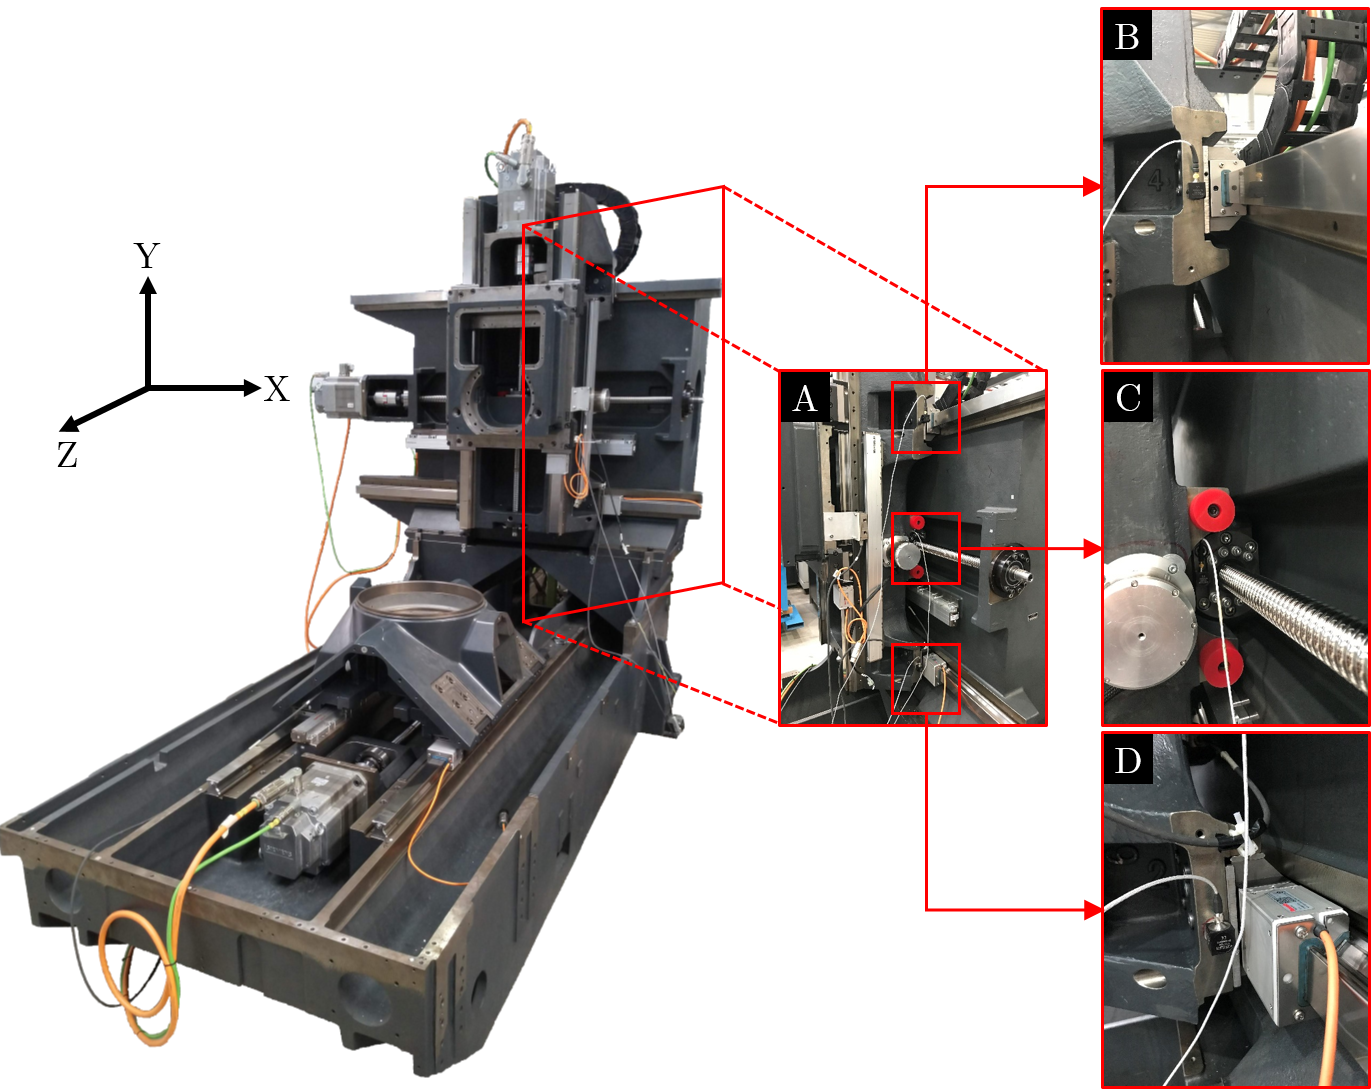
\includegraphics[width=0.9\textwidth]{experimental_setup}
  \caption {Experimental setup: A: side-view of the machine, B: upper LGS, C: threaded shaft of BSD, C: lower LGS}
  \label{fig:experimental_setup}
\end{figure}

\subsection{Sensors}
Signals from three different sources were included in the dataset. Three triaxial accelerometers recorded vibration signals and internal control data was accessed via the TNC Scope and TNC Opt. The recordings were triggered by different software programs, which were synchronized by a python script. Minor time delays between the signals could not be eliminated completely. Fig. \ref{fig:experimental_setup} shows the placement of the three triaxial Kistler 8762A10 piezo-eletric accelerometers at the upper LGS (sub-figure B), the BSD nut (sub-figure C) and the lower LGS (sub-figure D). The software tool TNC Scope was used to access the internal control data of the machine. TNC Opt is a software tool intended to optimize controllers. During the experiments, it was used to access those control data channels, which differed from those of TNC Scope.

\subsection{Definition of Health Condition Classes}
Preload classes (C1, C2, C3) were defined, specifying the preload level in BSDs and LGSs. For the BSDs also pitting damages were observed, which is why a separate pitting class (P) was defined. In total, four health condition classes were defined for the BSDs and three for the LGSs. The degradation of BSDs was specified by an ID containing one letter and either two digits for the preload classes or one digit for the pitting class. The degradation of LGSs was specified by an ID containing one letter and one digit. The letter indicates the damage types: no pitting (C) or pitting (P). The first digit in the BSD preload classes and the single digit in the LGS preload classes specify the preload level. The second digit in the BSD preload classes and the single digit in the BSD pitting class specify the observation. In the dataset, three distinct preload classes were defined. Based on the preload force (N), which was measured in the components, the recorded samples were assigned to those classes. Low preload forces result from high preload losses, which indicate strong component degradation. This lowers the precision of the machine and might lead to a complete machine failure. Preload class C3 was labeled as “healthy”, C2 as "slightly degraded" and C1 as "strongly degraded". Two sets of BSDs and one set of LGSs, each containing components of all corresponding health condition classes, were used during the data recording. To separate equally degraded BSDs from different sets, the observation digit was included in the BSD IDs. In total, ten recordings were made for each BSD and LGS combination. Table \ref{tab:recorded_combinations_of_LGS_and_BSD_health_conditions} shows all 24 combinations of differently degraded and observed BSDs and LGSs. In table \ref{tab:recorded_combinations_of_LGS_and_BSD_health_conditions} the numbers, indicating the specific BSD and LGS combinations, go up to 27. Originally the dataset included a third observation for the BSD preload class 3. In order to prevent a class imbalance, this observation was excluded from the experiments in this thesis. The forces specifying the different preload classes were defined differently for the observations. Table \ref {tab:BSDs_states} and table \ref {tab:LGSs_states} show all used BSDs and LGSs and their corresponding preload forces. Each experimental setup included two LGSs, each consisting of two counterparts, and one BSD. This is the reason, why in table \ref {tab:BSDs_states} each ID maps to one and in table \ref {tab:LGSs_states} to four preload forces.

\newpage

\begin{center}
\begin{longtable}{c c c} 
\toprule
 ID & Preload in N \\ [0.5ex] 
\midrule
 P1 & 2 070 \\ 
 P2 & 2 160 \\ 
 C11 & 950 \\ 
 C12 & 845 \\ 
 C21 & 1 450 \\ [1ex] 
 C22 & 1 293 \\ [1ex] 
 C31 & 2 390 \\ [1ex] 
 C32 & 2 328 \\ [1ex] 
\bottomrule
\caption {BSD health condition classes}
\label {tab:BSDs_states}
\end{longtable}
\end{center}

\begin{center}
\begin{longtable}{c c c} 
\toprule
 ID & Component & Preload in N \\ [0.5ex] 
\midrule
 C1 & C1 & 4 060 \\ 
    & C2 & 4 430 \\ 
    & C3 & 4 430 \\
    & F1 & 3 880 \\ 
\midrule
 C2 & B1 & 8 860 \\ 
    & B2 & 9 700 \\ [1ex] 
    & B3 & 9 070 \\ [1ex]
    & E1 & 8 230 \\ [1ex]
\midrule
 C3 & A9 & 13 470 \\ 
    & A10 & 14 530 \\ [1ex] 
    & A11 & 12 840 \\ [1ex]
    & D3 & 12 840 \\ [1ex]
\bottomrule
\caption {LGS health condition classes}
\label {tab:LGSs_states}
\end{longtable}
\end{center}

\begin{comment}
\begin{center}
\begin{longtable}{c c c c c c c c c c} 
\toprule
%\multicolumn{10}{c}{BSD}
&&&&BSD&&&&
\cmidrule(lr){3-11}
  & & C31 & C21 & C11 & P1 & C22 & C12 & C32 & P2  \\ [0.5ex] 
\cmidrule(lr){3-11}
                          & C1 & 1 & 2 & 3 & 4 & 5 & 6 & 7 & 9 \\ 
LGS                       & C2 & 10 & 11 & 12 & 13 & 14 & 15 & 16 & 18  \\ 
                          & C3 & 19 & 20 & 21 & 22 & 23 & 24 & 25 & 27  \\
\bottomrule
\caption {Combinations of LGS and BSD health condition states}
\label {tab:recorded_combinations_of_LGS_and_BSD_health_conditions}
\end{longtable}
\end{center}
\end{comment}






\begin{center}
\begin{longtable}{c c c c c c c c c c} 
\toprule
  &  &    &     &     &     \multicolumn{2}{c}{BSD}     &     &     &    \\ 
  &  & C31 & C21 & C11 & P1  & C22 & C12 & C32 & P2 \\ 
\midrule
     & \multicolumn{1}{c|}{C1} & 1 & 2 & 3 & 4 & 5 & 6 & 7 & 9 \\ 
 LGS & \multicolumn{1}{c|}{C2}& 10 & 11 & 12 & 13 & 14 & 15 & 16 & 18 \\  
     & \multicolumn{1}{c|}{C3} & 19 & 20 & 21 & 22 & 23 & 24 & 25 & 27 \\ 
\bottomrule
\caption {Combinations of LGS and BSD health condition classes}
\label {tab:recorded_combinations_of_LGS_and_BSD_health_conditions}
\end{longtable}
\end{center}


\subsection{Recording of Dataset}
For the sake of reproducibility, the experiments were executed with a fixed test cycle, which is defined in fig. \ref{fig:test_cycle}. Machine data was collected during constant speed, direction change and sweep excitation along the machine tool's X-axis. During the constant speed excitation, the machine tool was moved back and forth along the whole axis ($\Delta x$ = 600mm). During the direction change excitation, the movement of the machine tool was restricted to a small part of the axis ($\Delta x$ = 1mm) and the directions were changed with a high frequency. In the sweep excitation, the motor received a target speed in the form of a sine sweep. Before recording data, the machine was warmed up for 60min with a constant speed to create identical circumstances for all runs. For each experimental setup and speed excitation 10 experiments were recorded. 

\begin{figure}[H]
  \centering
  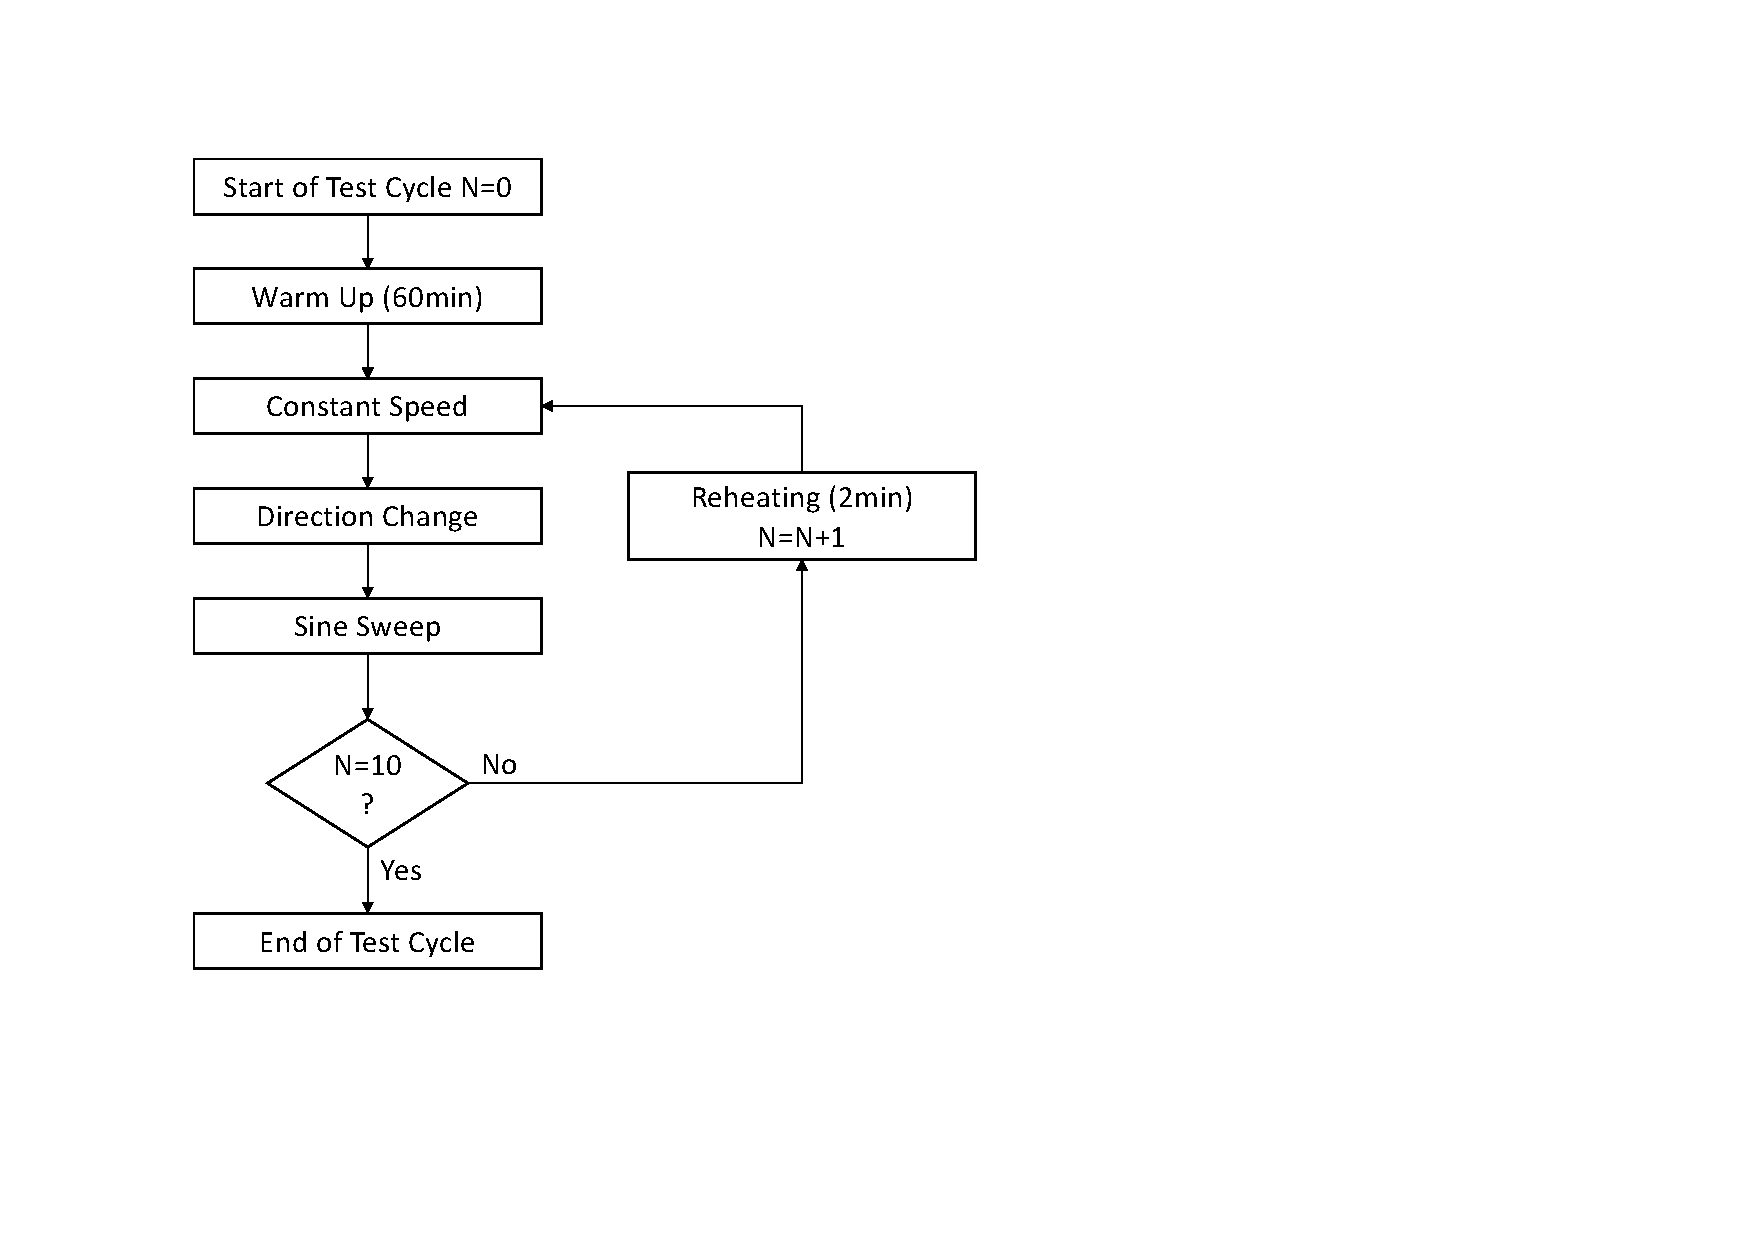
\includegraphics[width=0.7\textwidth]{test_cycle.pdf}
  \caption {Test cycle for data recording}
  \label{fig:test_cycle}
\end{figure}

In total 49 different signals were recorded. A more detailed specification of the signals can be found in the table. \ref{tab:description_of_the_49_recorded_features} in the appendix.

\subsection{Definition PHM Task on the Ball Screw Drive Dataset}
A binary health condition classification task was created by combining the BSD health condition classes C2 and C3 in a "healthy" and C1 and P1 in a "degraded" class. A domain shift was generated by combining all samples recorded with BSDs from observation 1 in the source and observation 2 in the target domain. Since the preload forces of BSDs were defined differently in both observations (see table \ref{tab:BSDs_states}), a domain shift is guaranteed. Additionally, marginal differences in the production and installation of the BSDs might increase the domain shift. The experiments of Li et al. \cite{Li2018} showed that the lifetime of BSDs is shorter than that of LGSs. This means that BSDs need to be replaced in shorter time intervals than LGSs. Therefore, it is very common that BSDs and LGSs with different levels of degradation are combined throughout the lifetime of industrial machines. This implies that the prediction of BSD health condition classes should not depend on the degradation level of LGSs. Usually, the training dataset contains just a limited number of observations of all health condition classes. Typically, the physical components available during training are different than those during testing. Nevertheless, both datasets contain samples from the same health condition classes. Therefore, it is essential to develop a robust PHM system, which can monitor the health condition of new and unseen components.

\section{Methods}\label{sec:methods}
The proposed model architecture and the corresponding training are presented in the following. All models applied to the dummy and real-world datasets have the same architecture. The model training partially deviated from the proposed one during the pre-evaluation of the approaches on the dummy dataset. In chapter \ref{sec:results_dummy_dataset}, the training variations are specified in more detail. 

\subsection{Model}
\label{sec:model}
The architecture of the proposed PHM model consists of a one-dimensional CNN and a subsequent classifier. A detailed visualization of the architecture is shown in fig. \ref{fig:proposed_model}. The CNN extracts expressive features, which are later used by the classifier to predict the health condition of the BSDs. The CNN consists of three convolutional layers. Throughout the network, the spatial dimension of the feature map is decreased and its depth increased. This helps extracting more global features in shallow and more specific and local features in deeper layers. The exact parameters of the convolutional layers are specified in table \ref{tab:parameter_conv} 
\begin{longtable}{c c c c} 
\toprule
Parameter & Conv 1 & Conv 2 & Conv 3 \\
\midrule
kernel size & 100 & 10 & 5 \\

padding size & 0 & 1 & 1 \\

stride & 1 & 1 & 1 \\
\bottomrule
\caption {Parameters in convolutional layer}
\label {tab:parameter_conv}
\end{longtable}

In order to reduce the spatial dimension of the feature maps, pooling layers are included after the convolutional layers. This reduction of the model complexity prevents problems like overfitting and exploding gradients. Batch normalization is applied after the convolutional layers. For each batch, the means and variances of the layer's input are fixed, which makes the training faster and more stable. After iteratively applying these three types of layers, the output of the CNN is flattened and normalized to a one-dimensional vector. This vector is fed to the subsequent classifier. The latent feature space dimensions of the classifier are reduced constantly. In the end, the probability for the two defined BSD health condition classes is predicted.


\begin{figure}[H]
  \centering
  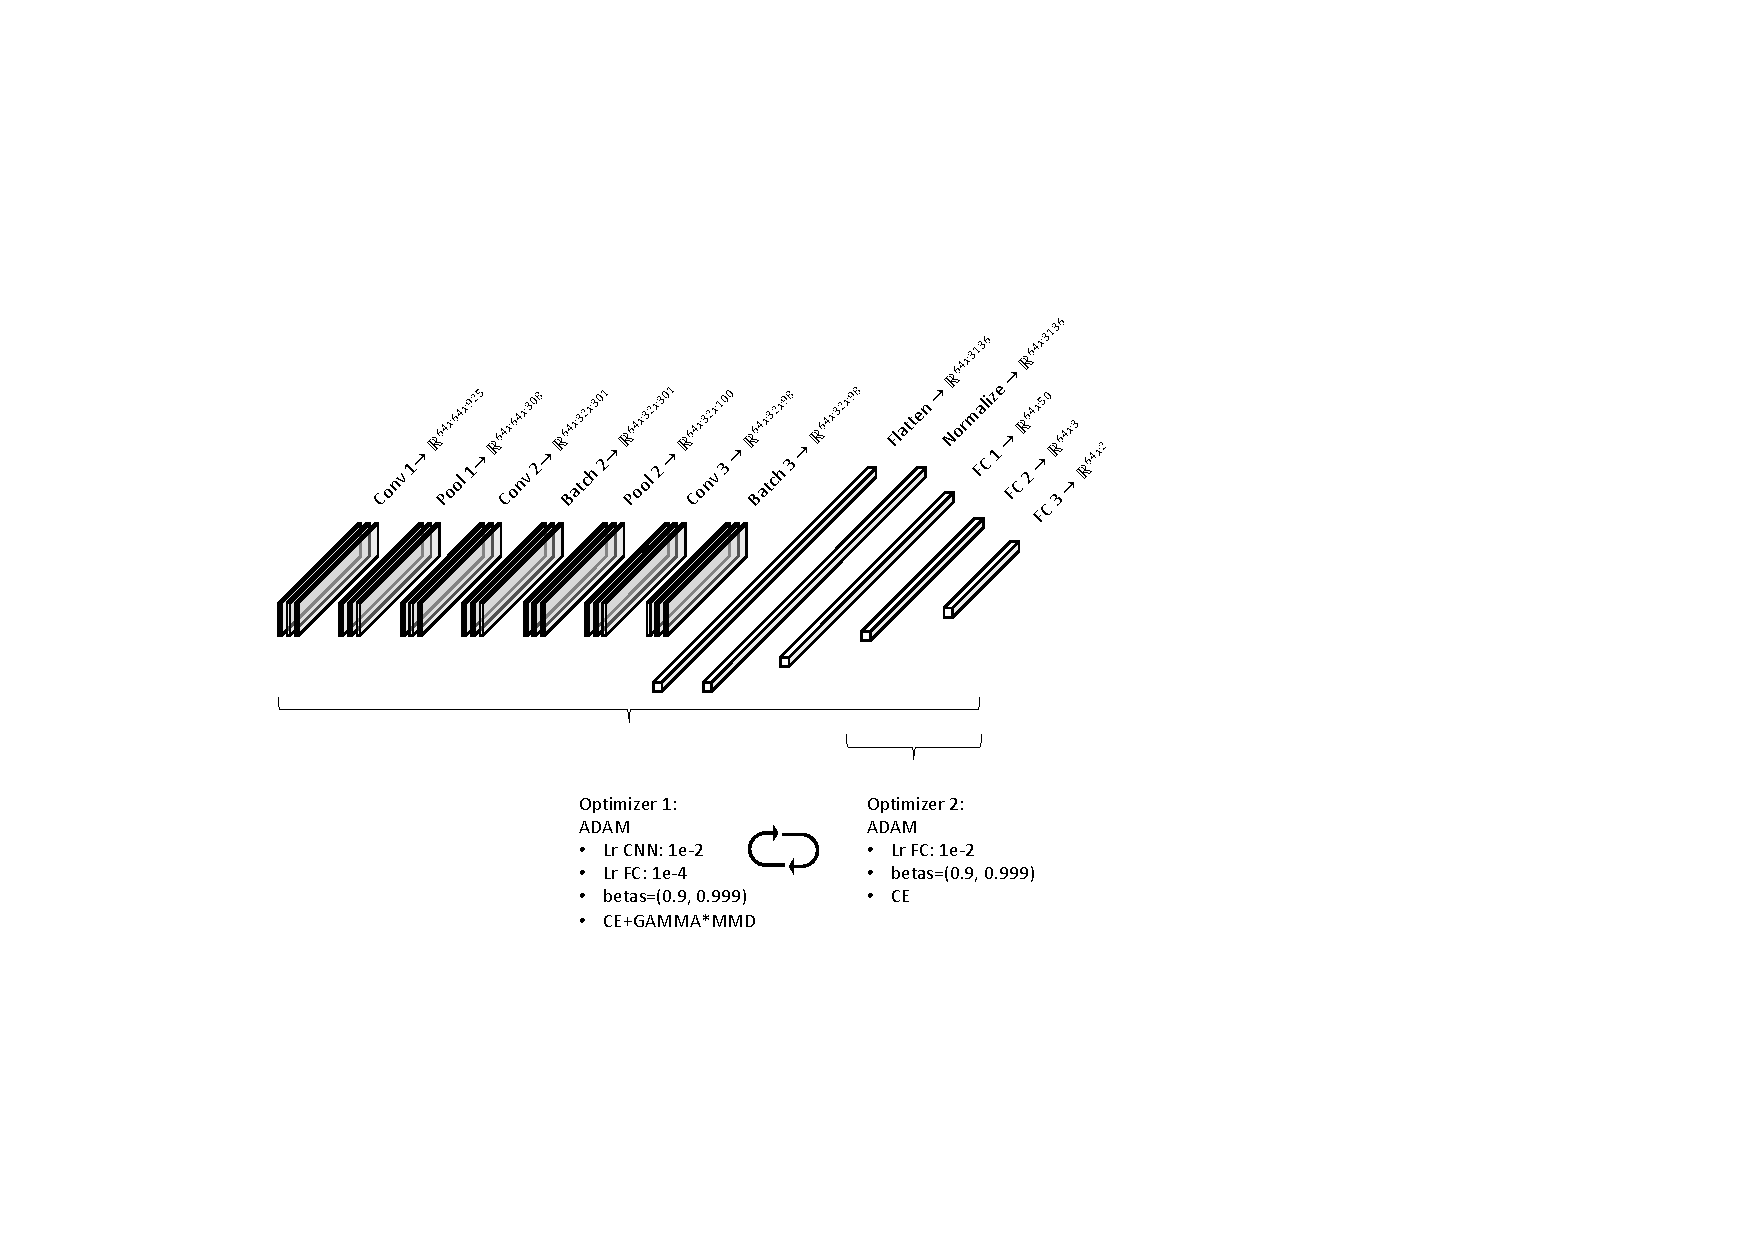
\includegraphics[width=1\textwidth]{proposed_model.pdf}
  \caption {Proposed model architecture} \label{fig:proposed_model}
\end{figure}


\subsection{Proposed Training with MMD- and CE-Loss} \label{sec:Proposed_training}

In the first step, the data used for the training is pre-processed. In the course of that, the dataloader separates the data into shorter sequences of length 1024. These windows, which can include several of the recorded 49 signals, are fed to the model as single samples. The sequenced signals are cleaned from Nan values and synchronized afterward. Separate source and target domain dataloader split the corresponding datasets into four different parts: MMD-Training (40\%), CE-Training (20\%), Validation (20\%) and Testing (20\%). Other pre-processing steps, like wavelet transforms, can easily be added to the dataloader. The repetitive training of the model is visualized in fig. \ref{fig:Training_Process_MMD}. The model training is separated into two phases. In the first phase, a weighted average of CE- and MMD-loss is used to optimize the whole network: 
\begin{equation}
    \mbox{Total Loss} = \mbox{Source CE-Loss} + \mbox{GAMMA} \cdot \mbox{MMD-Loss}, 
\end{equation}
where GAMMA is a hyperparameter balancing the influence of the CE- and MMD-loss, which needs to be defined beforehand. Different learning rates in the feature extractor and classifier allow the training intensity to be adjusted separately for the different modules. In this phase, an ADAM optimizer is applied with a learning rate of 1e-2 in the layers Conv1 - FC1 and a learning rate of 1e-4 in the layers FC2 - FC3. In the second phase, just the CE-loss is applied to optimize the layers FC2 - FC3. Again an ADAM optimizer with a learning rate of 1e-2 is used. In both optimization steps, the beta values are 0.9 and 0.999. Two-thirds of the training data is used in the first and one-third in the second training phase. The application of the two different optimizers is visualized in fig. \ref{fig:proposed_model}. The MMD-loss estimates the domain discrepancy in the latent feature maps of the neural network. The MMD-loss facilitates the extraction of domain invariant features. The domain discrepancy is measured as the squared distance between the distribution kernel embeddings in the reproducing kernel Hilbert space (RKHS). The kernel choice is of great importance for the performance of the MMD-loss. By combining several RBF kernels with bandwidth parameters 1, 2, 4, 8, 16, the model training profits from their individual strength. The source and target samples are randomly coupled up and processed by the MMD-loss. The classes of these samples are not considered in the MMD-loss. Therefore, the MMD-loss minimizes the domain discrepancy between the source and target domain of different and equal classes. The MMD-loss is applied in several layers of the feature extractor and classifier. The source CE-loss optimizes the model to increase the classification accuracy on the source domain. Fig. \ref{fig:MMD_Loss_and_CE_loss} symbolically shows how the MMD and the source CE-loss are applied in different model layers. The training is repeated until the maximum number of epochs is reached. After the training is completed, the model can be used to predict the BSD health condition classes of unseen target domain samples. 



\begin{figure}[H]
  \centering
  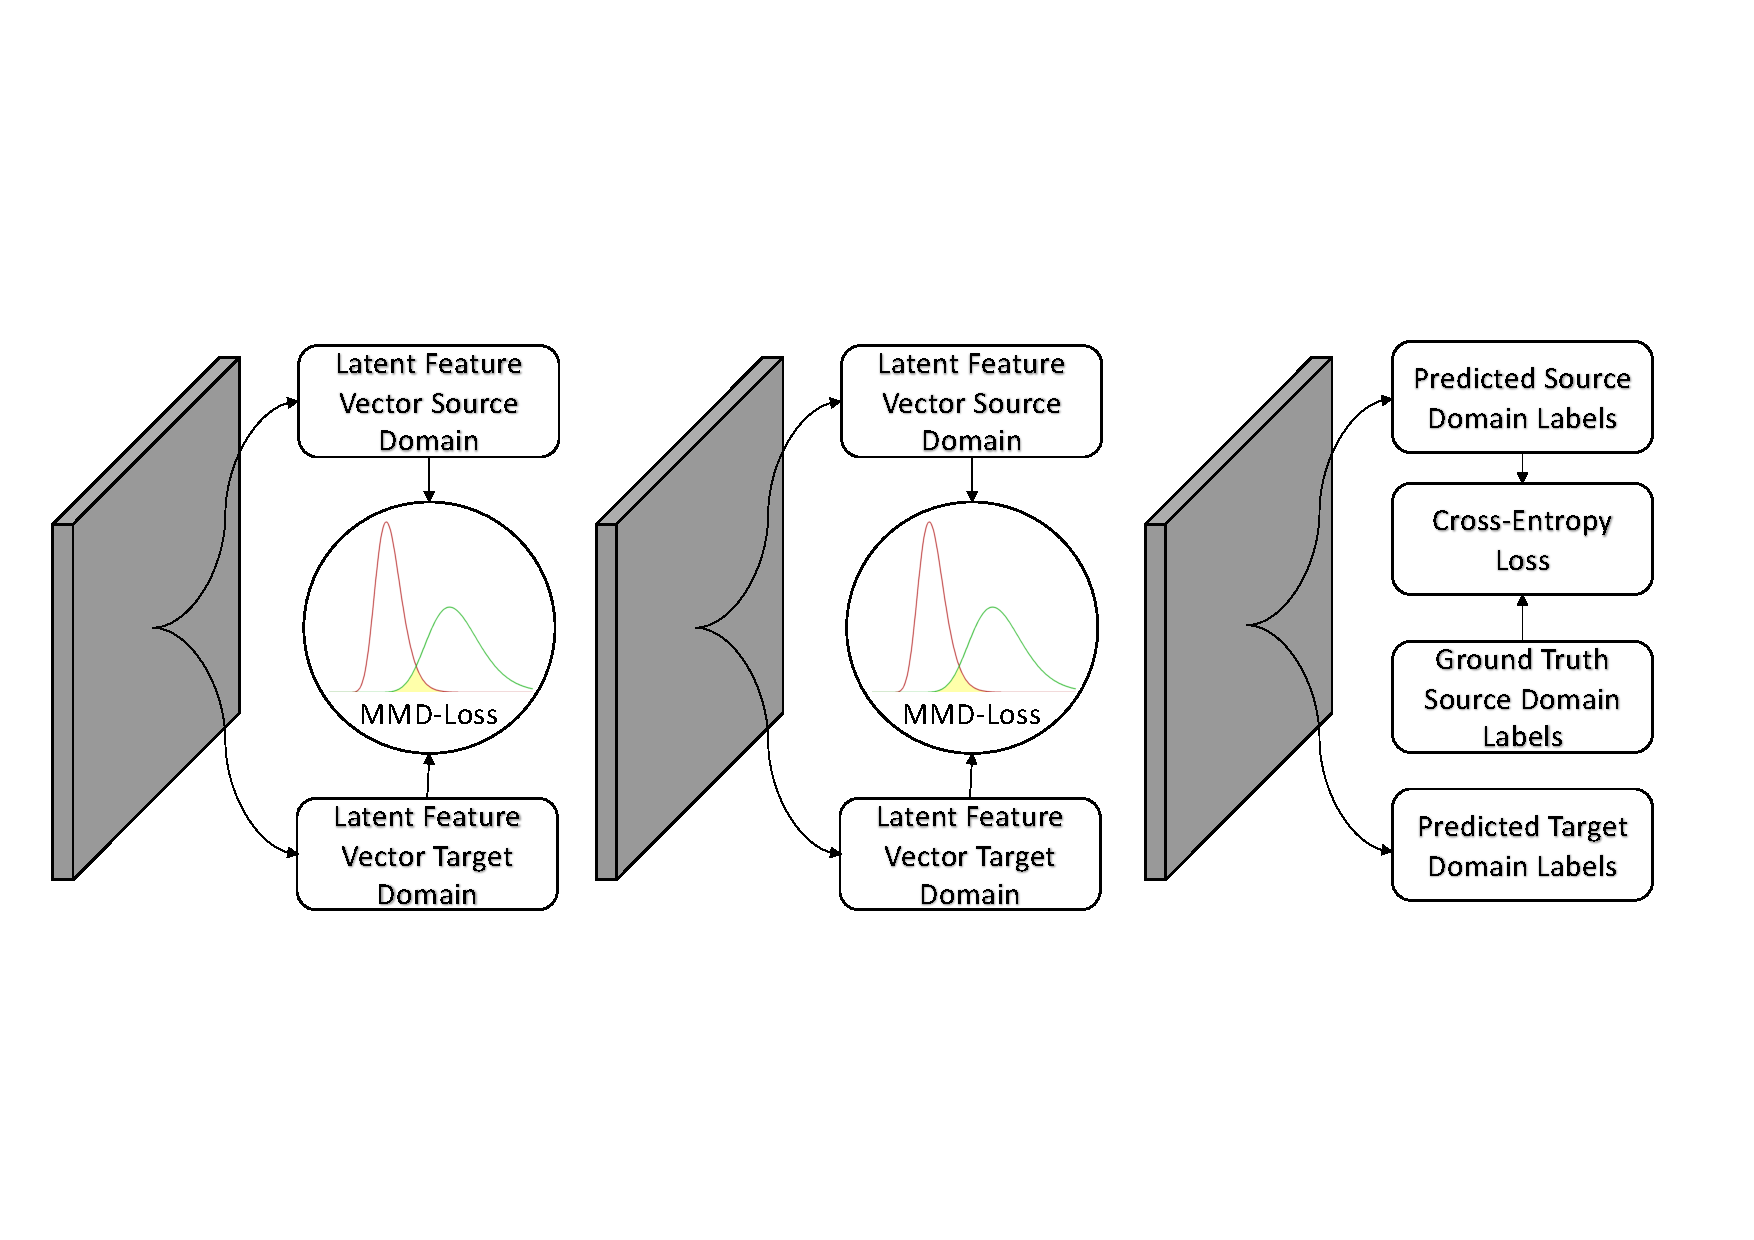
\includegraphics[width=1\textwidth]{MMD_loss_visualization.pdf}
  \caption {Application of CE- and MMD-loss during optimization of neural networks} \label{fig:MMD_Loss_and_CE_loss}
\end{figure}

\begin{figure}[H]
  \centering
  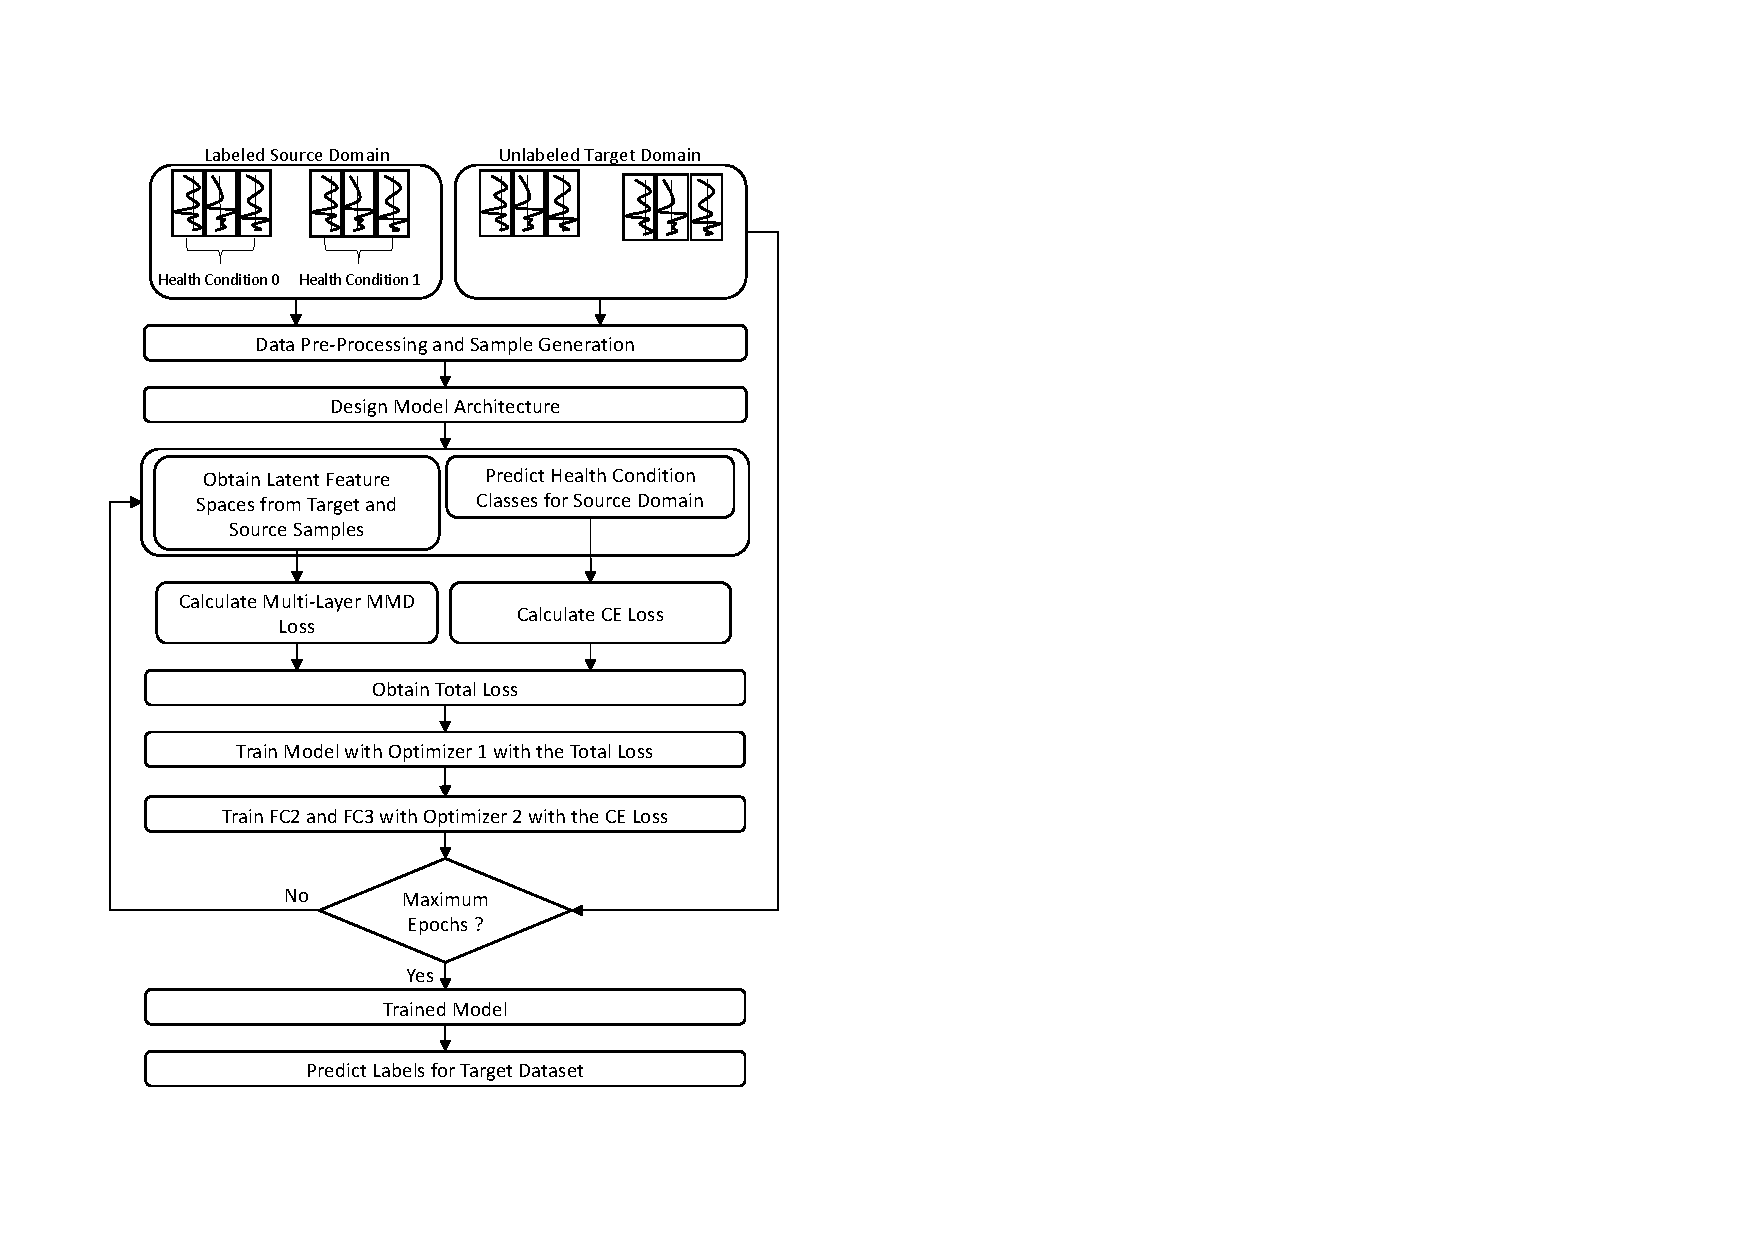
\includegraphics[width=0.8\textwidth]{training_process_mmd.pdf}
  \caption {Model training and testing} \label{fig:Training_Process_MMD}
\end{figure}


\chapter{Results}\label{chapter:results}
In the research community, simplified synthetically generated datasets are quite common to understand the underlying functionalities and mechanisms of new approaches and to evaluate their applicability for a given task. For the sake of completeness, it is necessary to test these approaches on real-world data. If that is done correctly, one can estimate the robustness and actual benefit of the approach for the real-world task. In the following, the results from different experiments on the dummy and real-world BSD datasets are described.

\section{Dummy Dataset}\label{sec:results_dummy_dataset}
Several experiments were performed on the dummy dataset to analyze the effects of the MMD-loss in a simplified setting and to make first estimates about its applicability in the PHM context. The model architecture used in these experiments was the same as described in section \ref{sec:model}. The model described in chapter \ref{cnn_mmd_dummy} was optimized as explained in section \ref{sec:Proposed_training}. In the experiments of section \ref{sec:Balancing Cross-Entropy and MMD loss} and \ref{sec:Differences of labeled and unlabeled MMD loss} the models were optimized with a single SGD optimizer and a learning rate of 0.01. In those two experiments, all layers were trained simultaneously with a weighted average of an MMD- and source CE-loss.

\subsection{Influence of GAMMA Choice on the Domain Adaptation Performance} \label{sec:Balancing Cross-Entropy and MMD loss}

The following section evaluates the influence of the weighting factor GAMMA on the training. The latent feature representations of the source and target samples in the FC2 layer are visualized in fig. \ref{fig:point_cloud_mmd}. The development of the MMD and CE-loss throughout the training are shown in fig. \ref{fig:learning_curves_influence_mmd_feature_extractor}.
\begin{itemize}
    \item [\textbf{Small GAMMA}]:
    When picking a very small GAMMA, the model can not increase the compactness and separability of the class representations in the latent feature maps. Besides that, the class representations do not overlap well for the two domains (see fig. \ref{fig:point_cloud_mmd}). For this GAMMA choice, the source CE-loss dominates the training. Instead of reducing the domain discrepancy, the model training focuses solely on predicting source samples correctly. The model can accurately predict the source domain labels but can not transfer that knowledge to the target domain. The CE-loss can be reduced very efficiently, whereas the MMD-loss increases throughout the training (see fig. \ref{fig:learning_curves_influence_mmd_feature_extractor}).
    \item [\textbf{Medium GAMMA}]:
    When GAMMA is chosen correctly, the source CE- and MMD-loss can be reduced simultaneously (see fig. \ref{fig:learning_curves_influence_mmd_feature_extractor}). A trade-off is found, where the model is optimized to correctly classify the source domain samples while reducing the domain discrepancy. Knowledge learned from the source domain is successfully transferred to the target domain. In this case, the training profits from both losses equally. An optimization with multiple goals is achieved and none of them solely dominates the training. The class distributions in the latent feature space show increased compactness and separability for both domains. The overlap between both domains is improved (see fig. \ref{fig:point_cloud_mmd}).
    \item [\textbf{Large GAMMA}]:
    When picking a very large GAMMA, the training is dominated by the MMD-loss. The correct prediction of source domain samples becomes irrelevant during the training. Since the target labels are unknown, the MMD-loss is calculated between source and target samples of the same as well as different classes. Therefore, the MMD-loss reduces the inter- and intra-class distance between the latent feature representations of the source and target domain. The compactness of the classes is increased but the separability is reduced. The optimization ends in a trivial solution, where all latent feature representations collapse to a point- or needle-like subspace (see \ref{fig:point_cloud_mmd}). The model reduces the distance between the samples of all classes and domains without aiming to solve the classification task. Throughout the training, the MMD-loss is reduced and the CE-loss increased (see fig. \ref{fig:learning_curves_influence_mmd_feature_extractor}).
\end{itemize}

\begin{figure}[H]
  \centering
  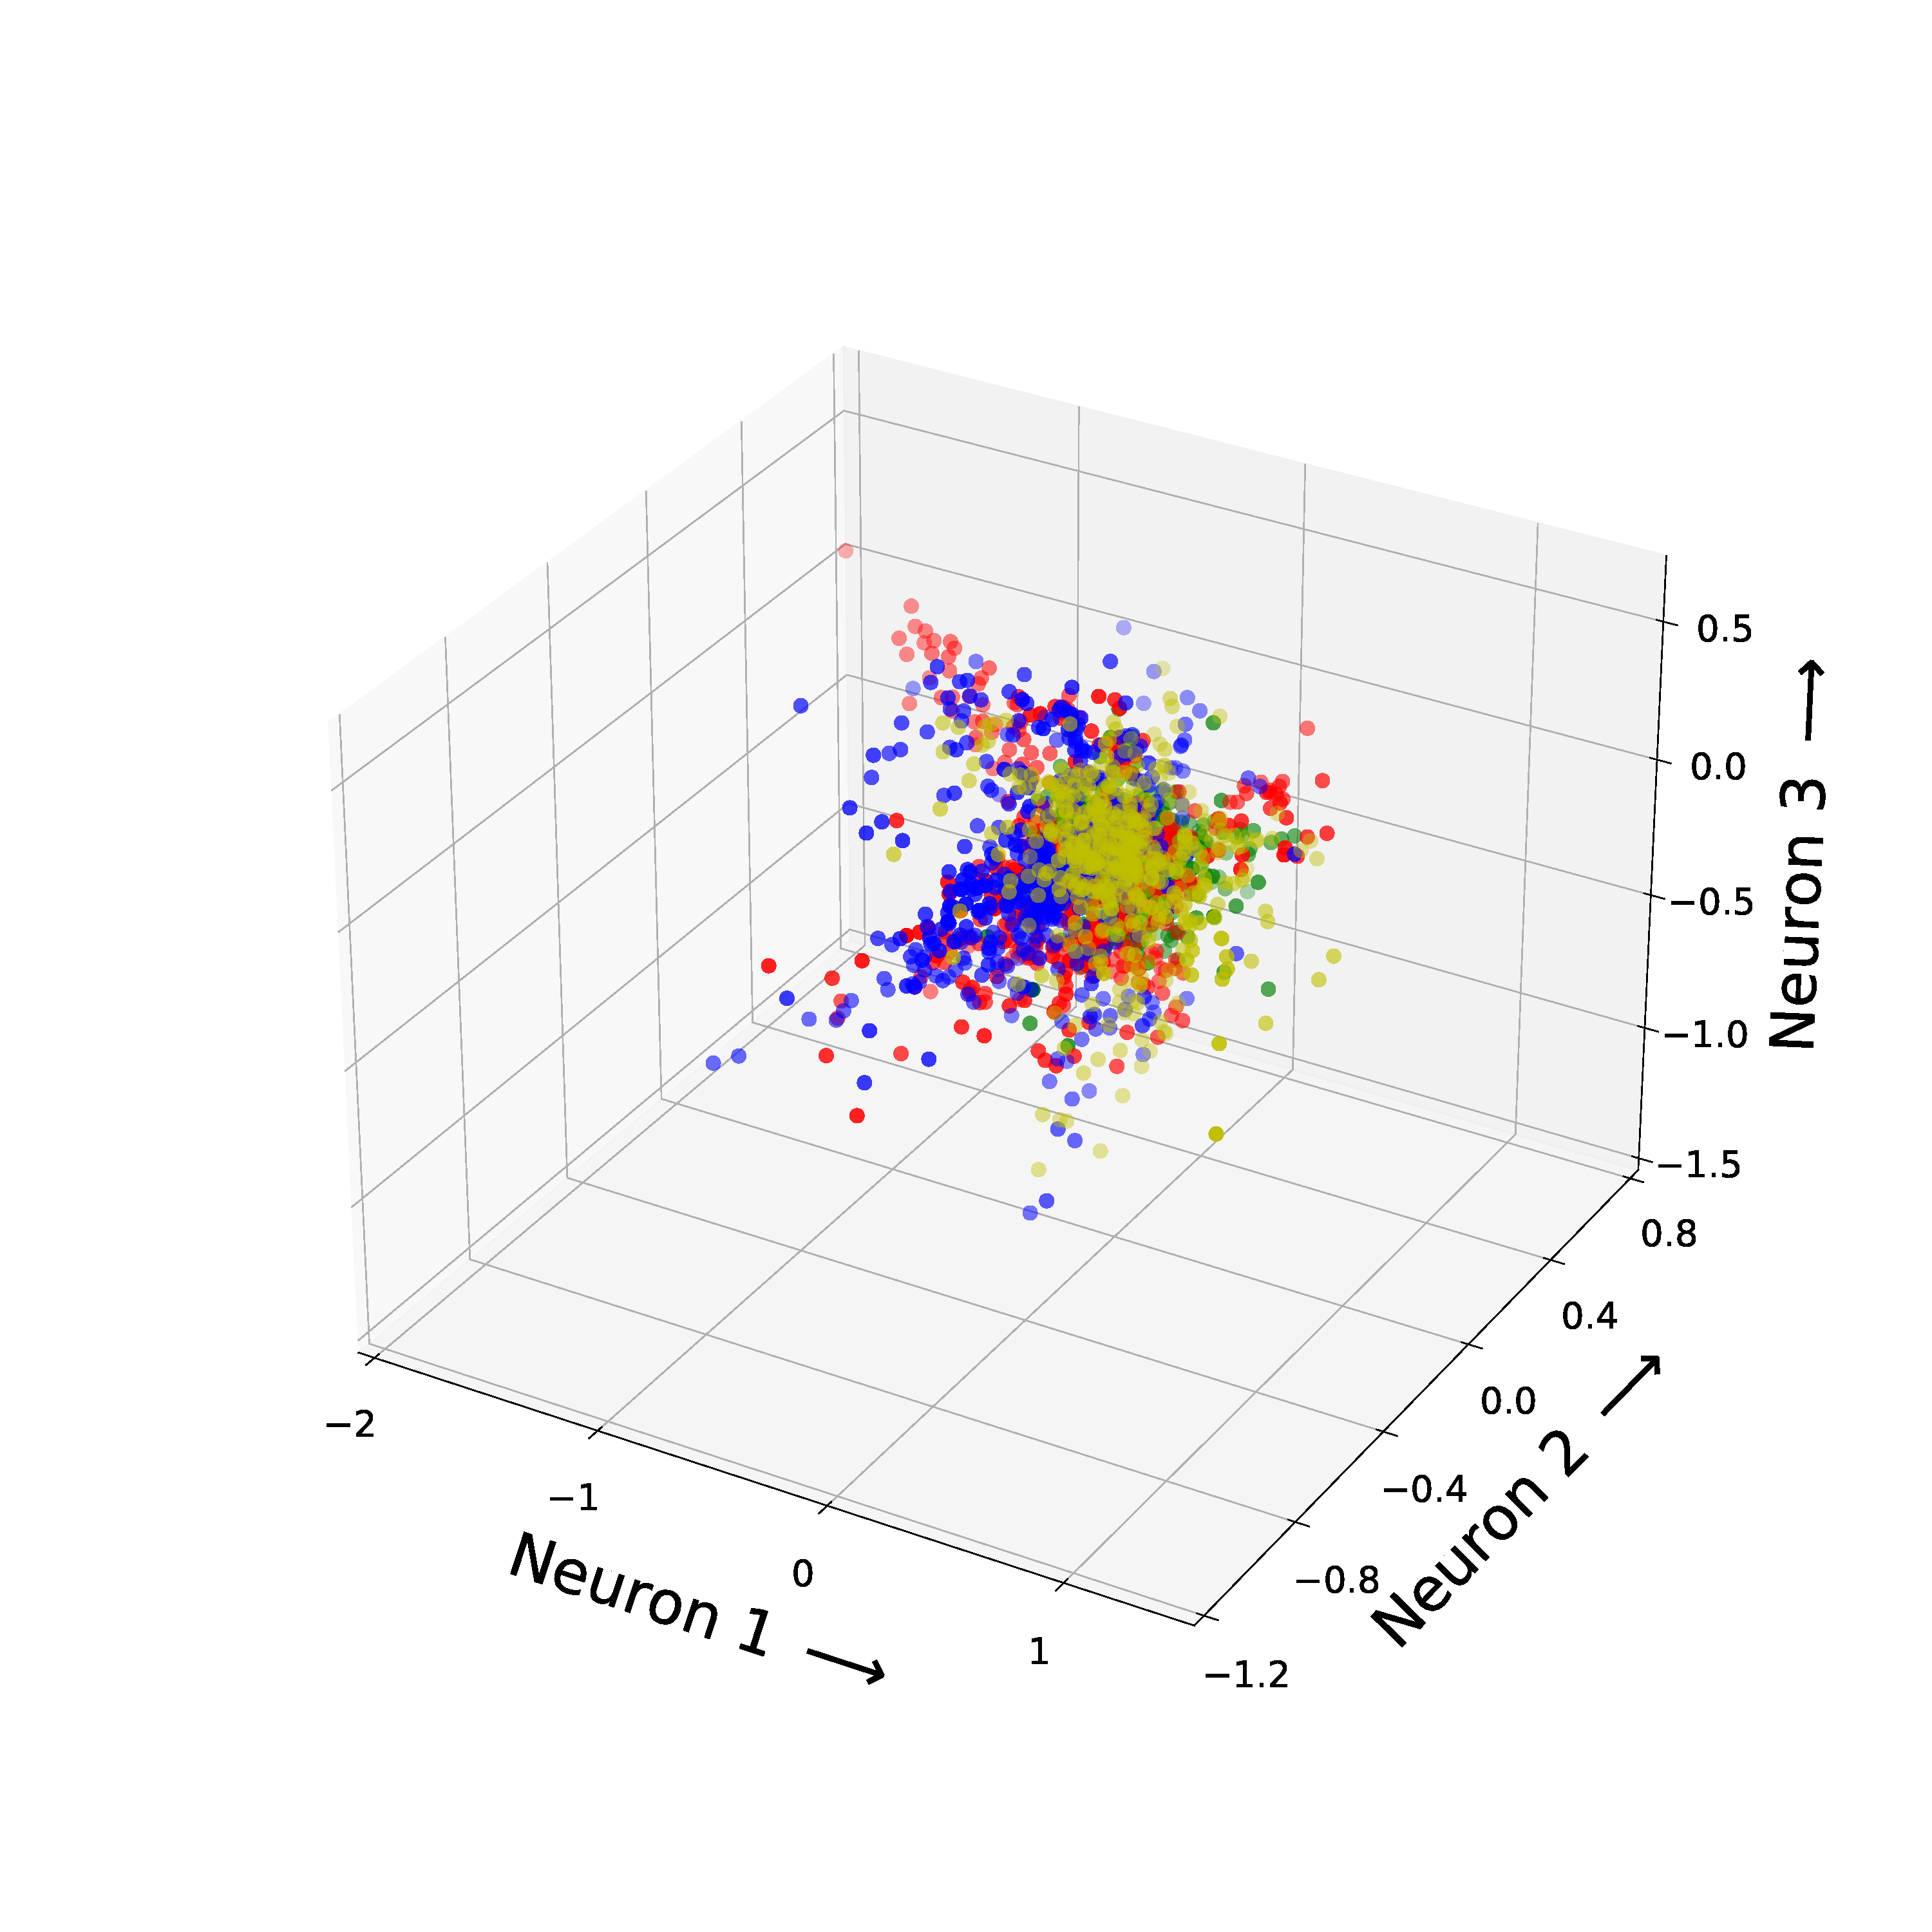
\includegraphics[width=.48\textwidth]{GAMMA_Influence_dummy_distribution/Dummy_distribution_0_GAMMA_0_001.pdf}
  \hspace{.4cm}
  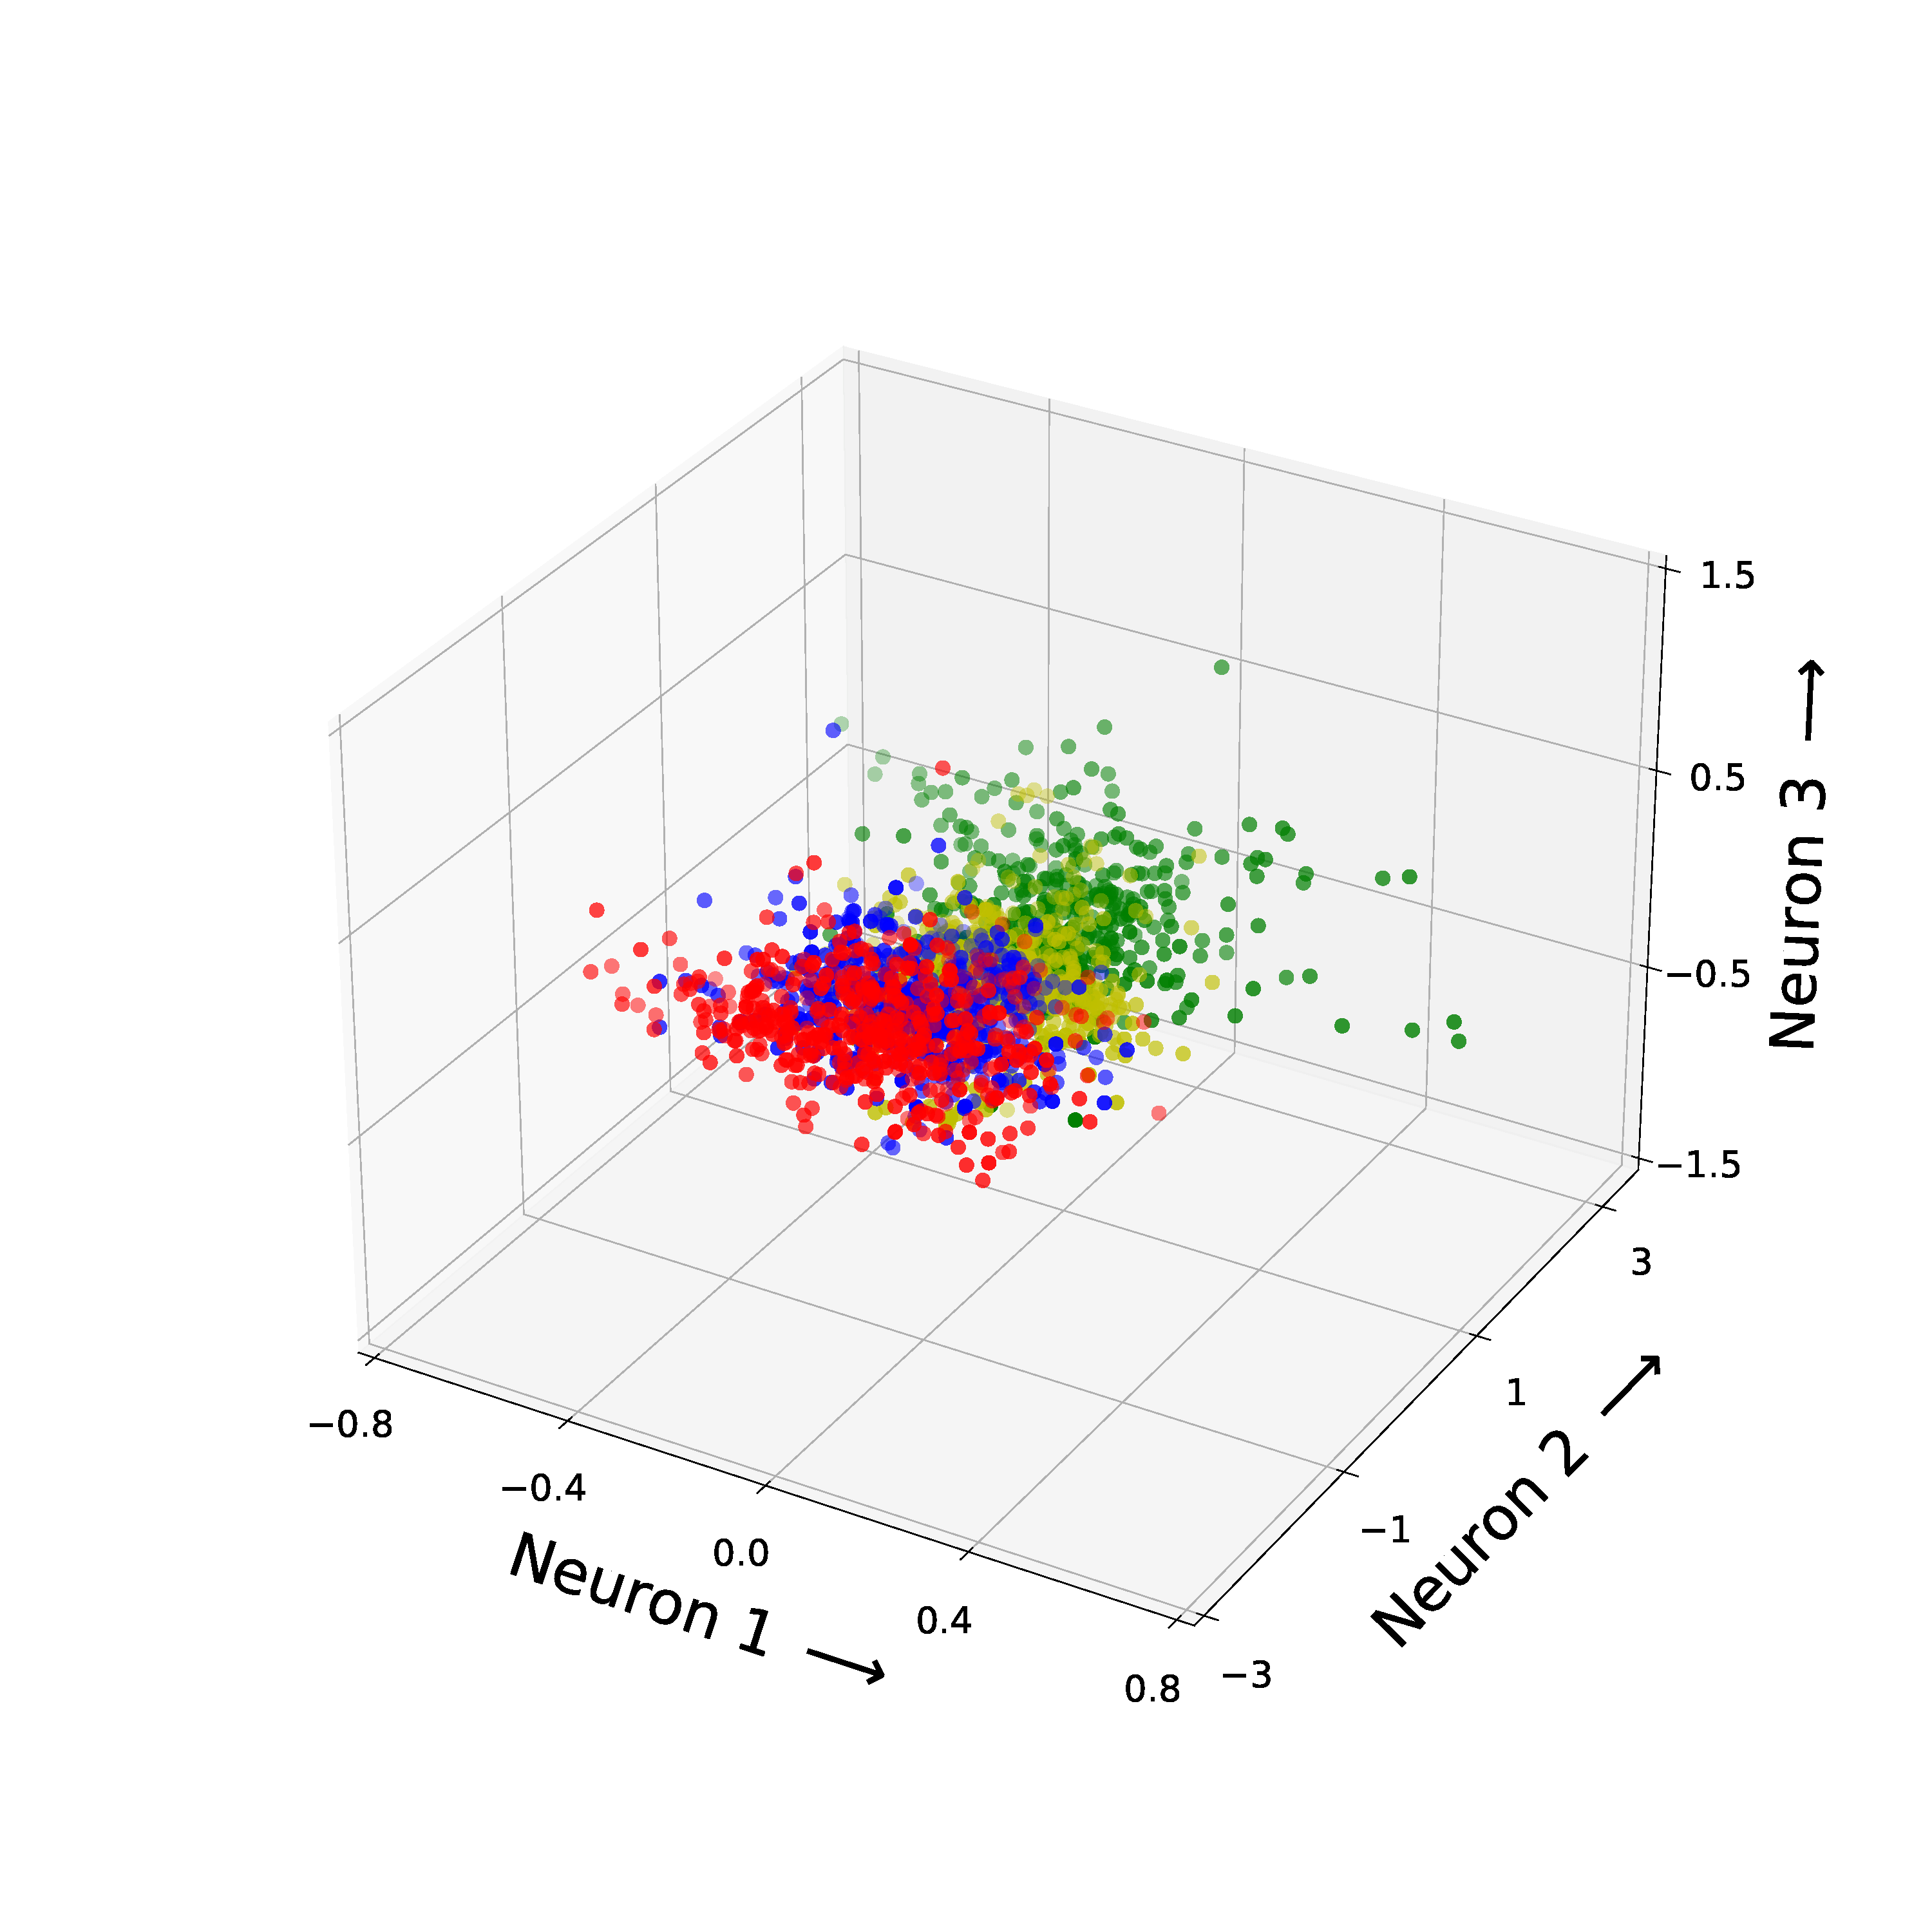
\includegraphics[width=.48\textwidth]{GAMMA_Influence_dummy_distribution/Dummy_distribution_8_GAMMA_0_001.pdf}

  \vspace{.1cm}

  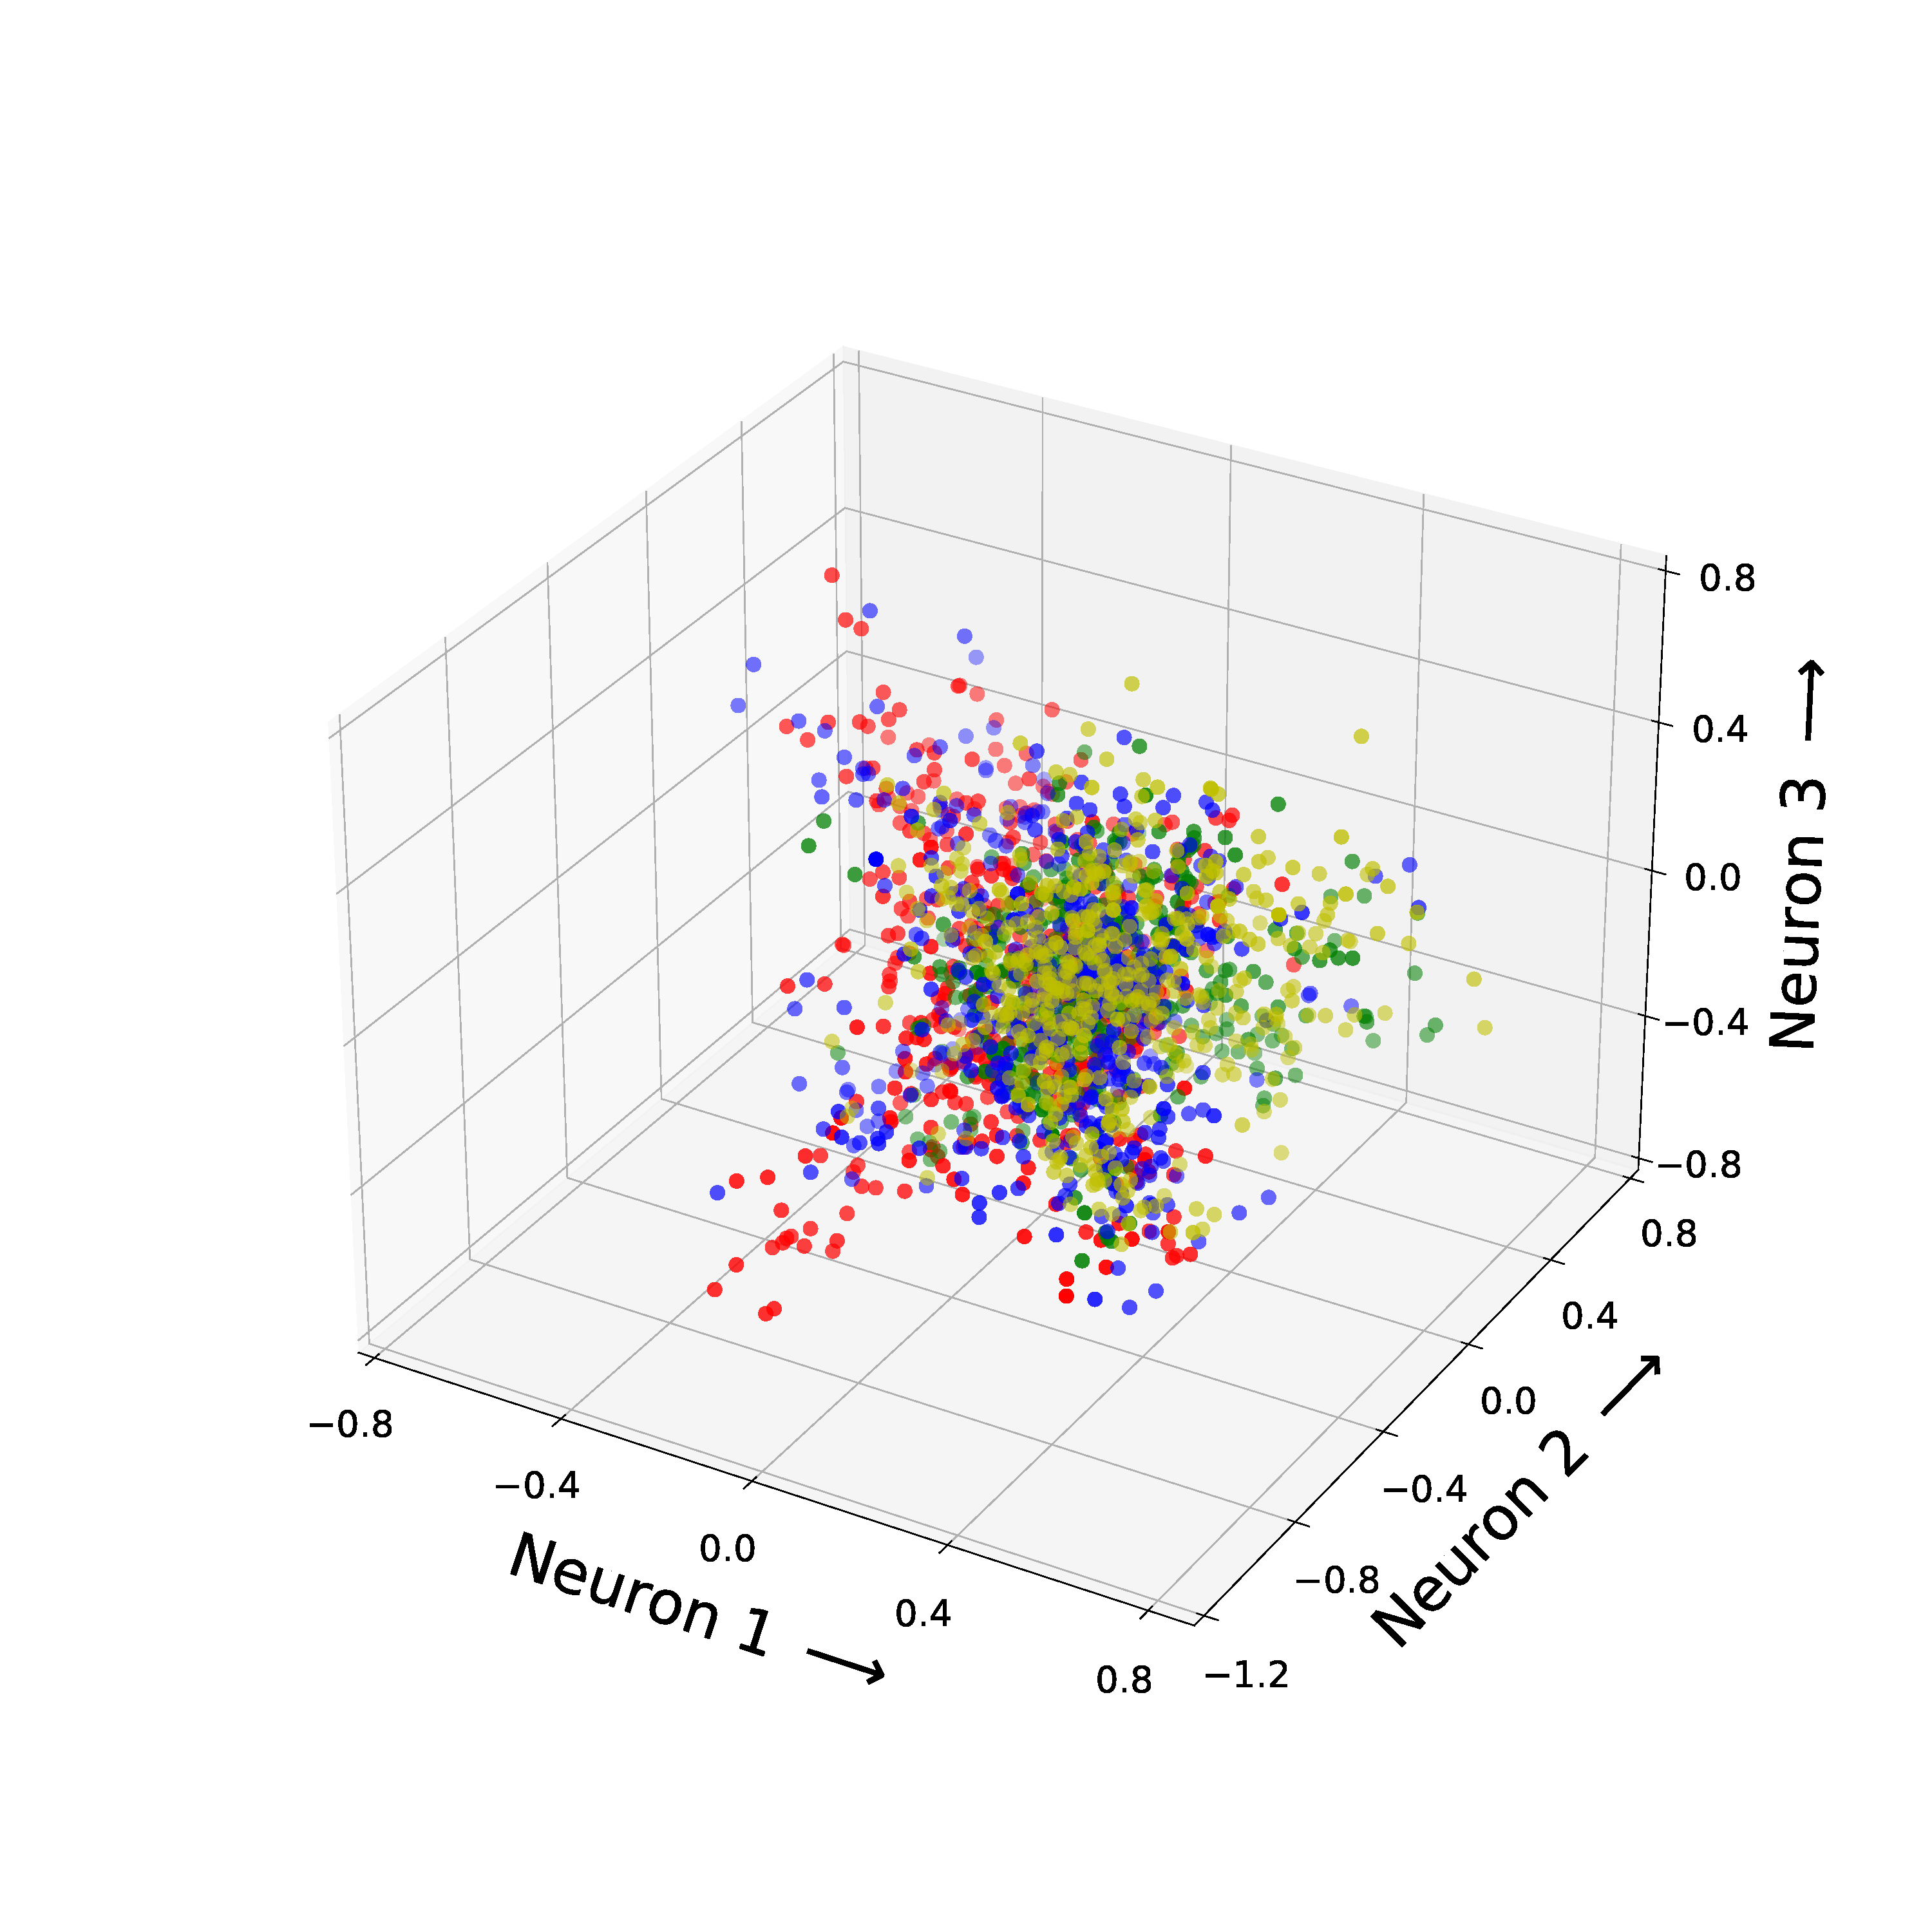
\includegraphics[width=.48\textwidth]{GAMMA_Influence_dummy_distribution/Dummy_distribution_0_GAMMA_0_1.pdf}
  \hspace{.4cm}
  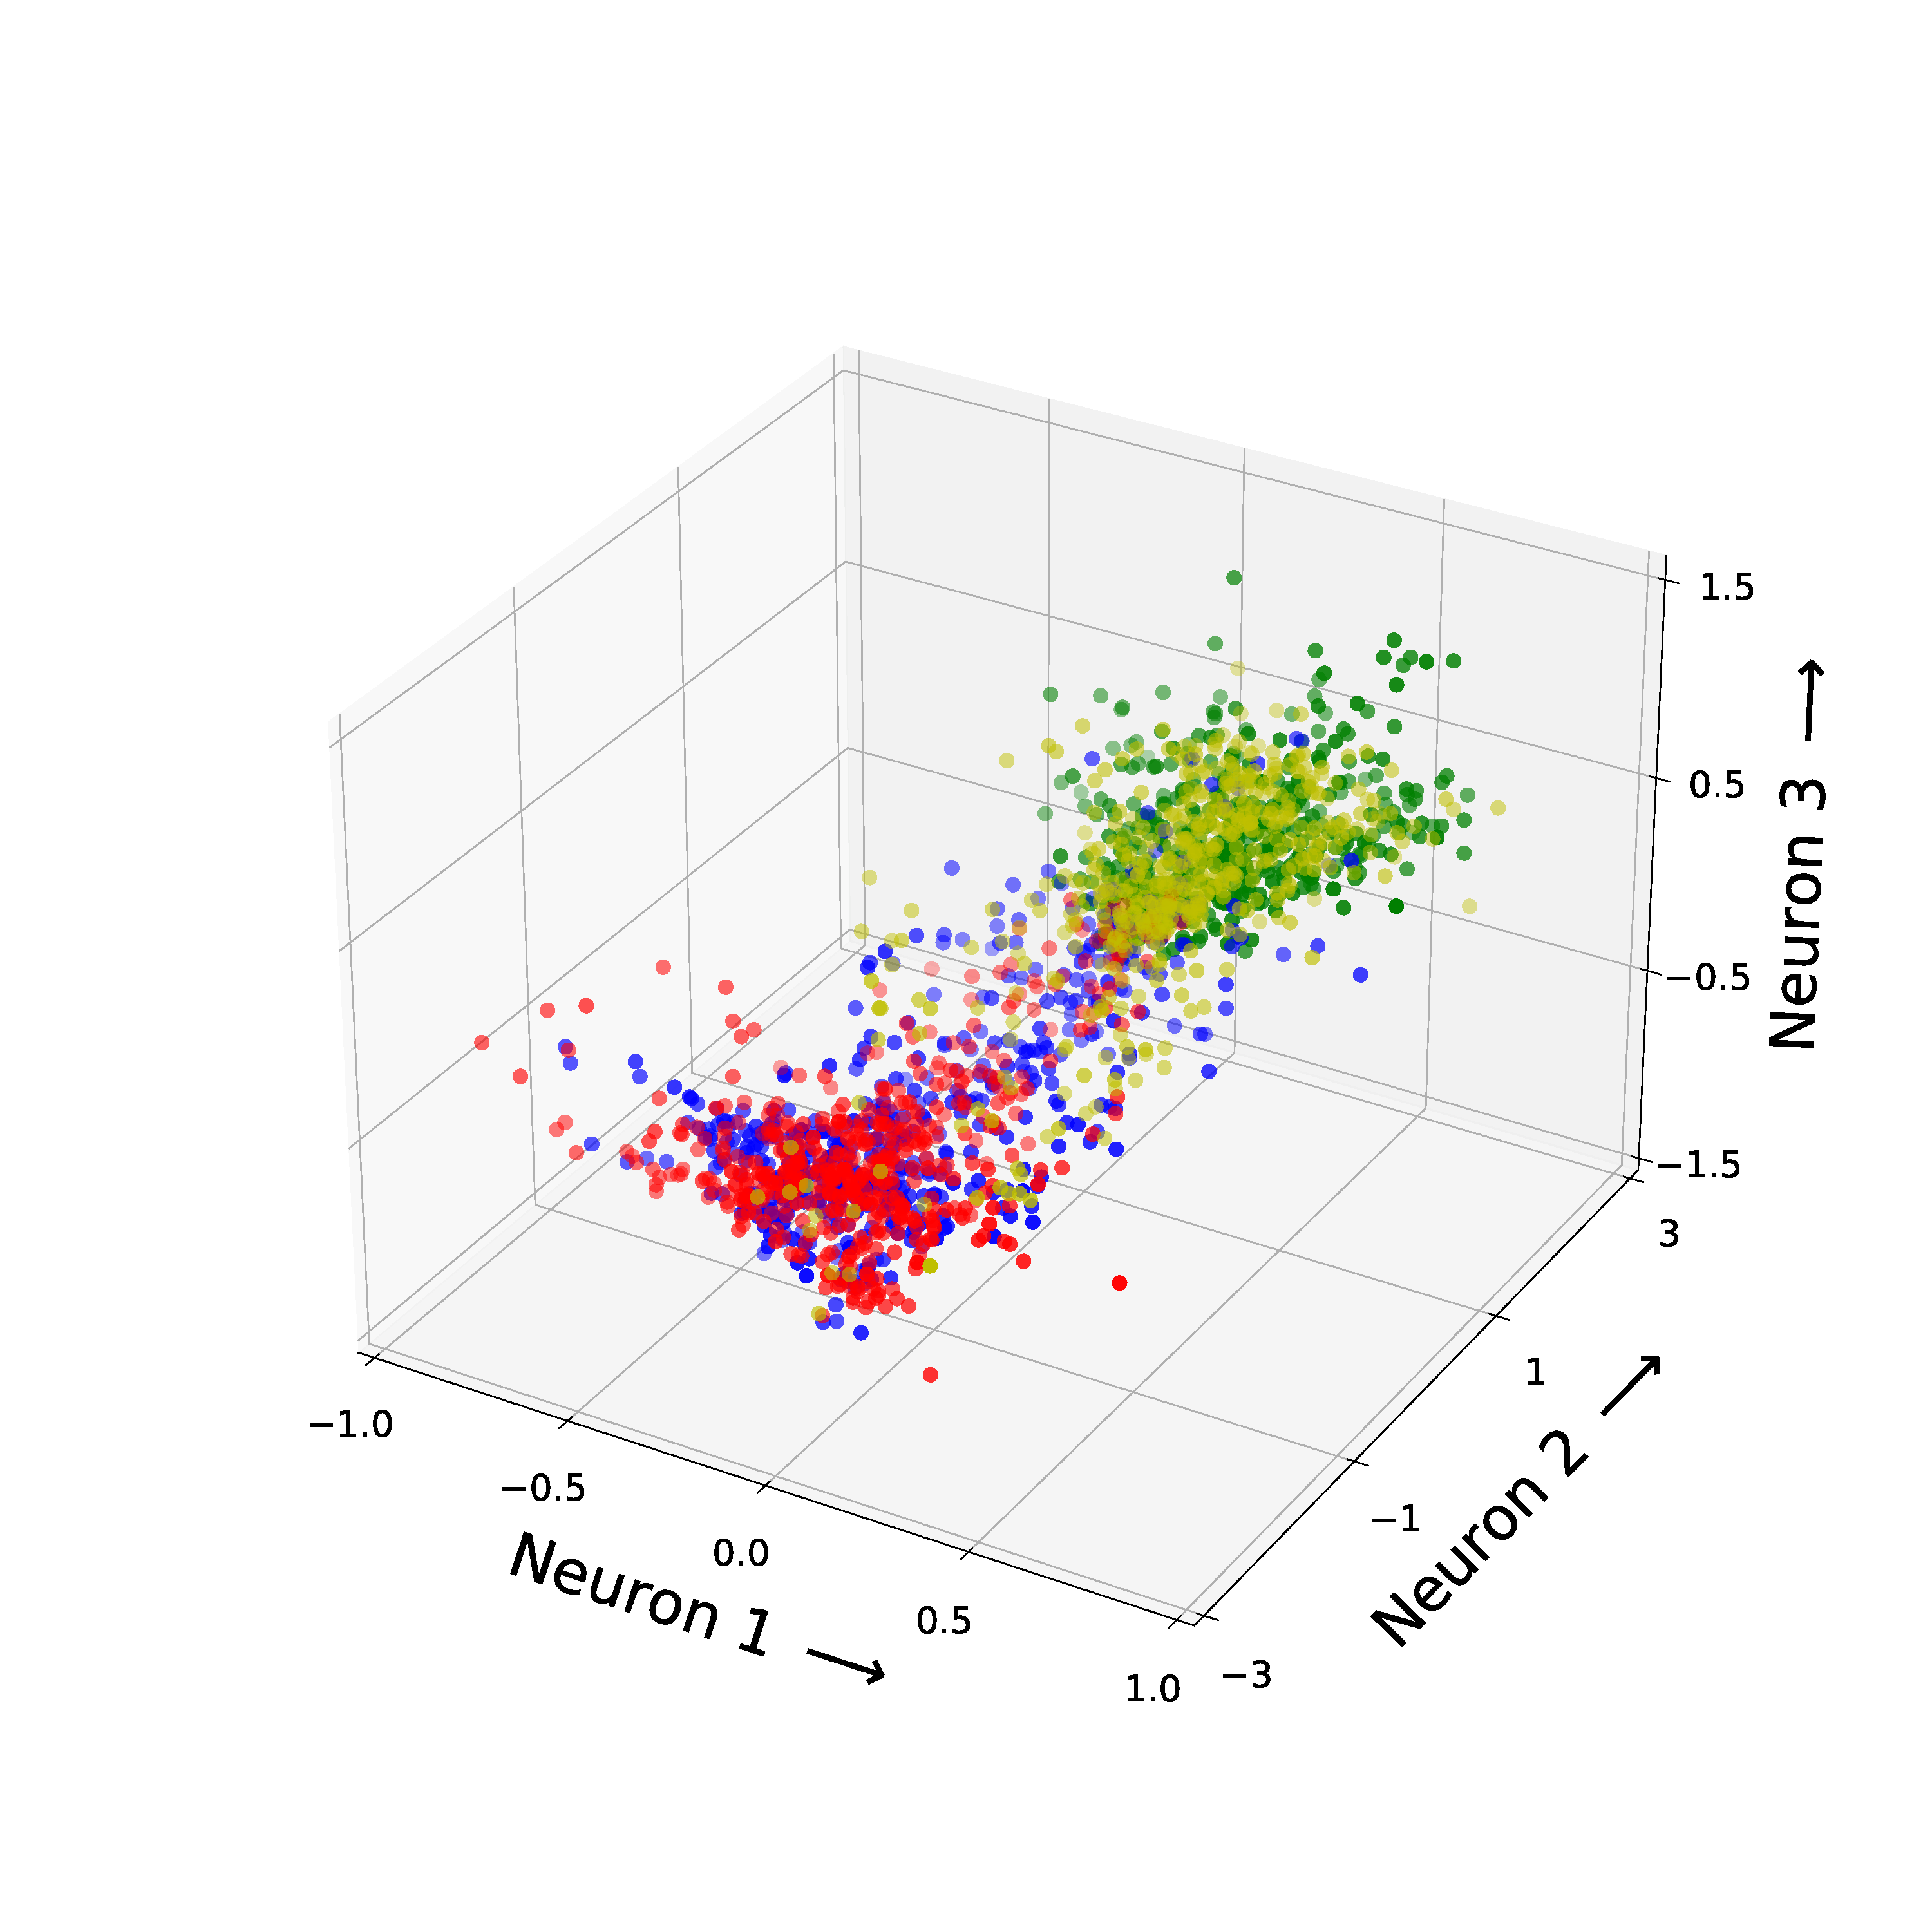
\includegraphics[width=.48\textwidth]{GAMMA_Influence_dummy_distribution/Dummy_distribution_8_GAMMA_0_1.pdf}

  \vspace{.1cm}

  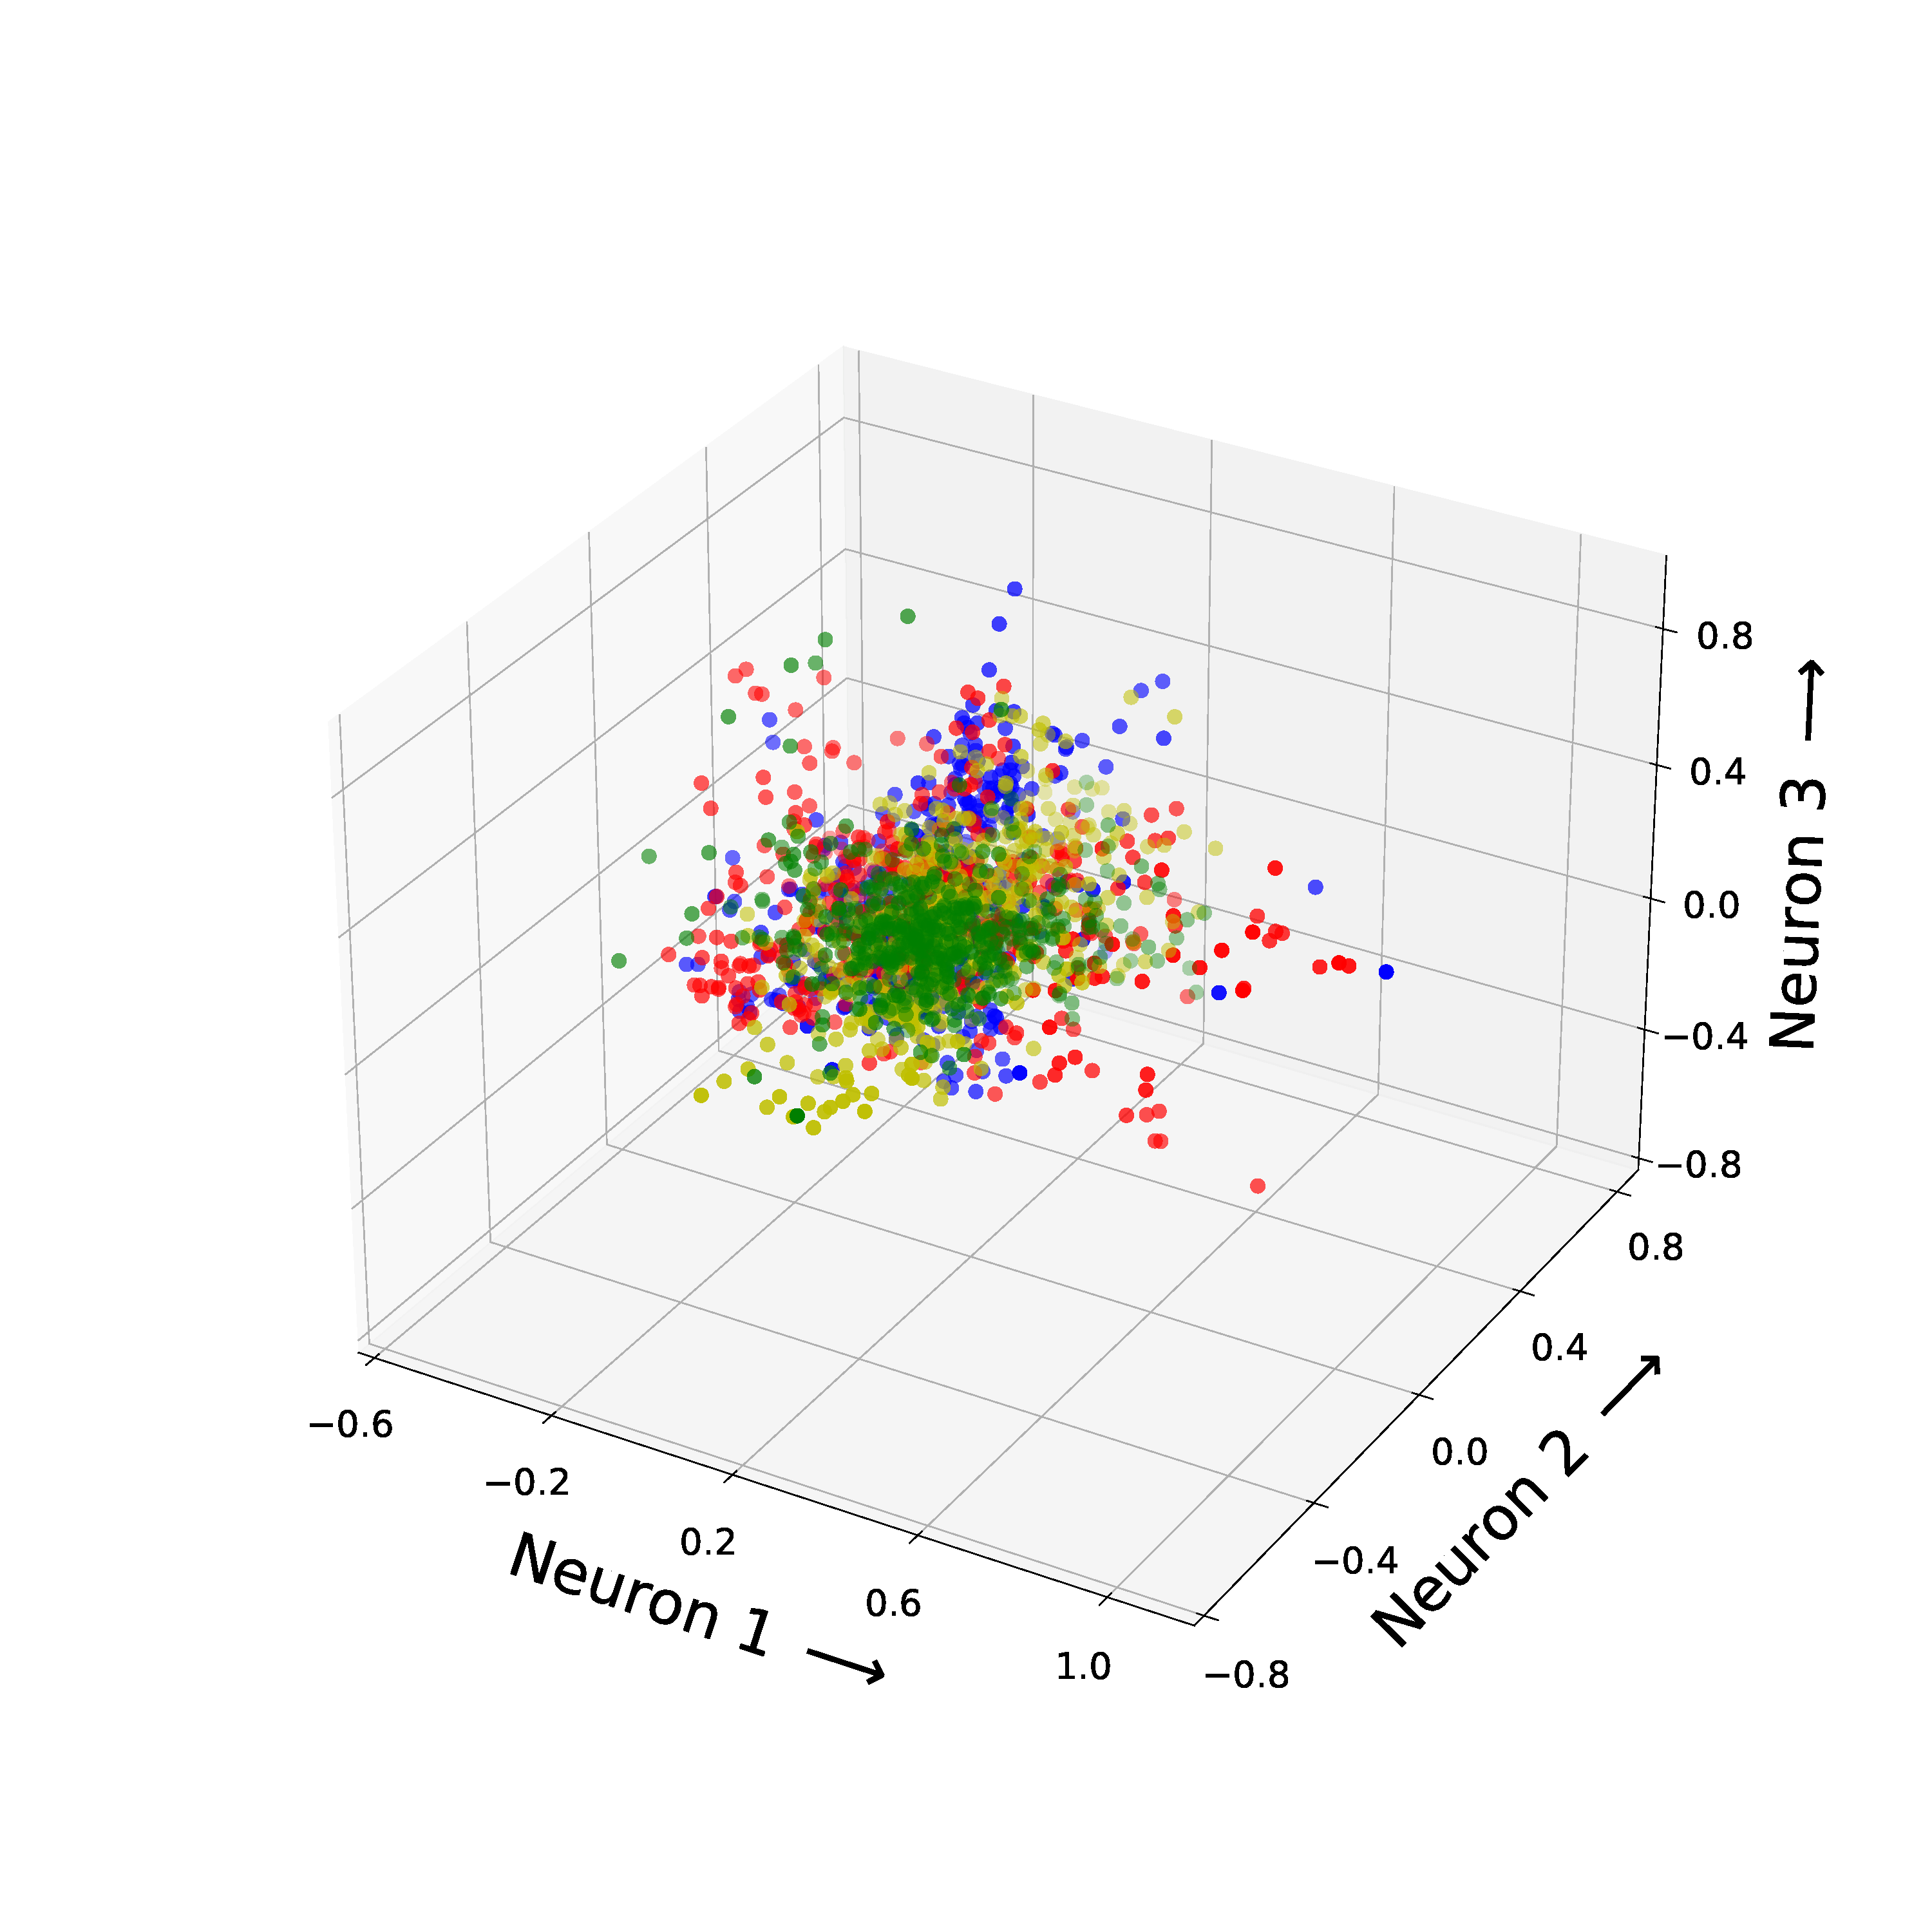
\includegraphics[width=.48\textwidth]{GAMMA_Influence_dummy_distribution/Dummy_distribution_0_GAMMA_20.pdf}
  \hspace{.4cm}
  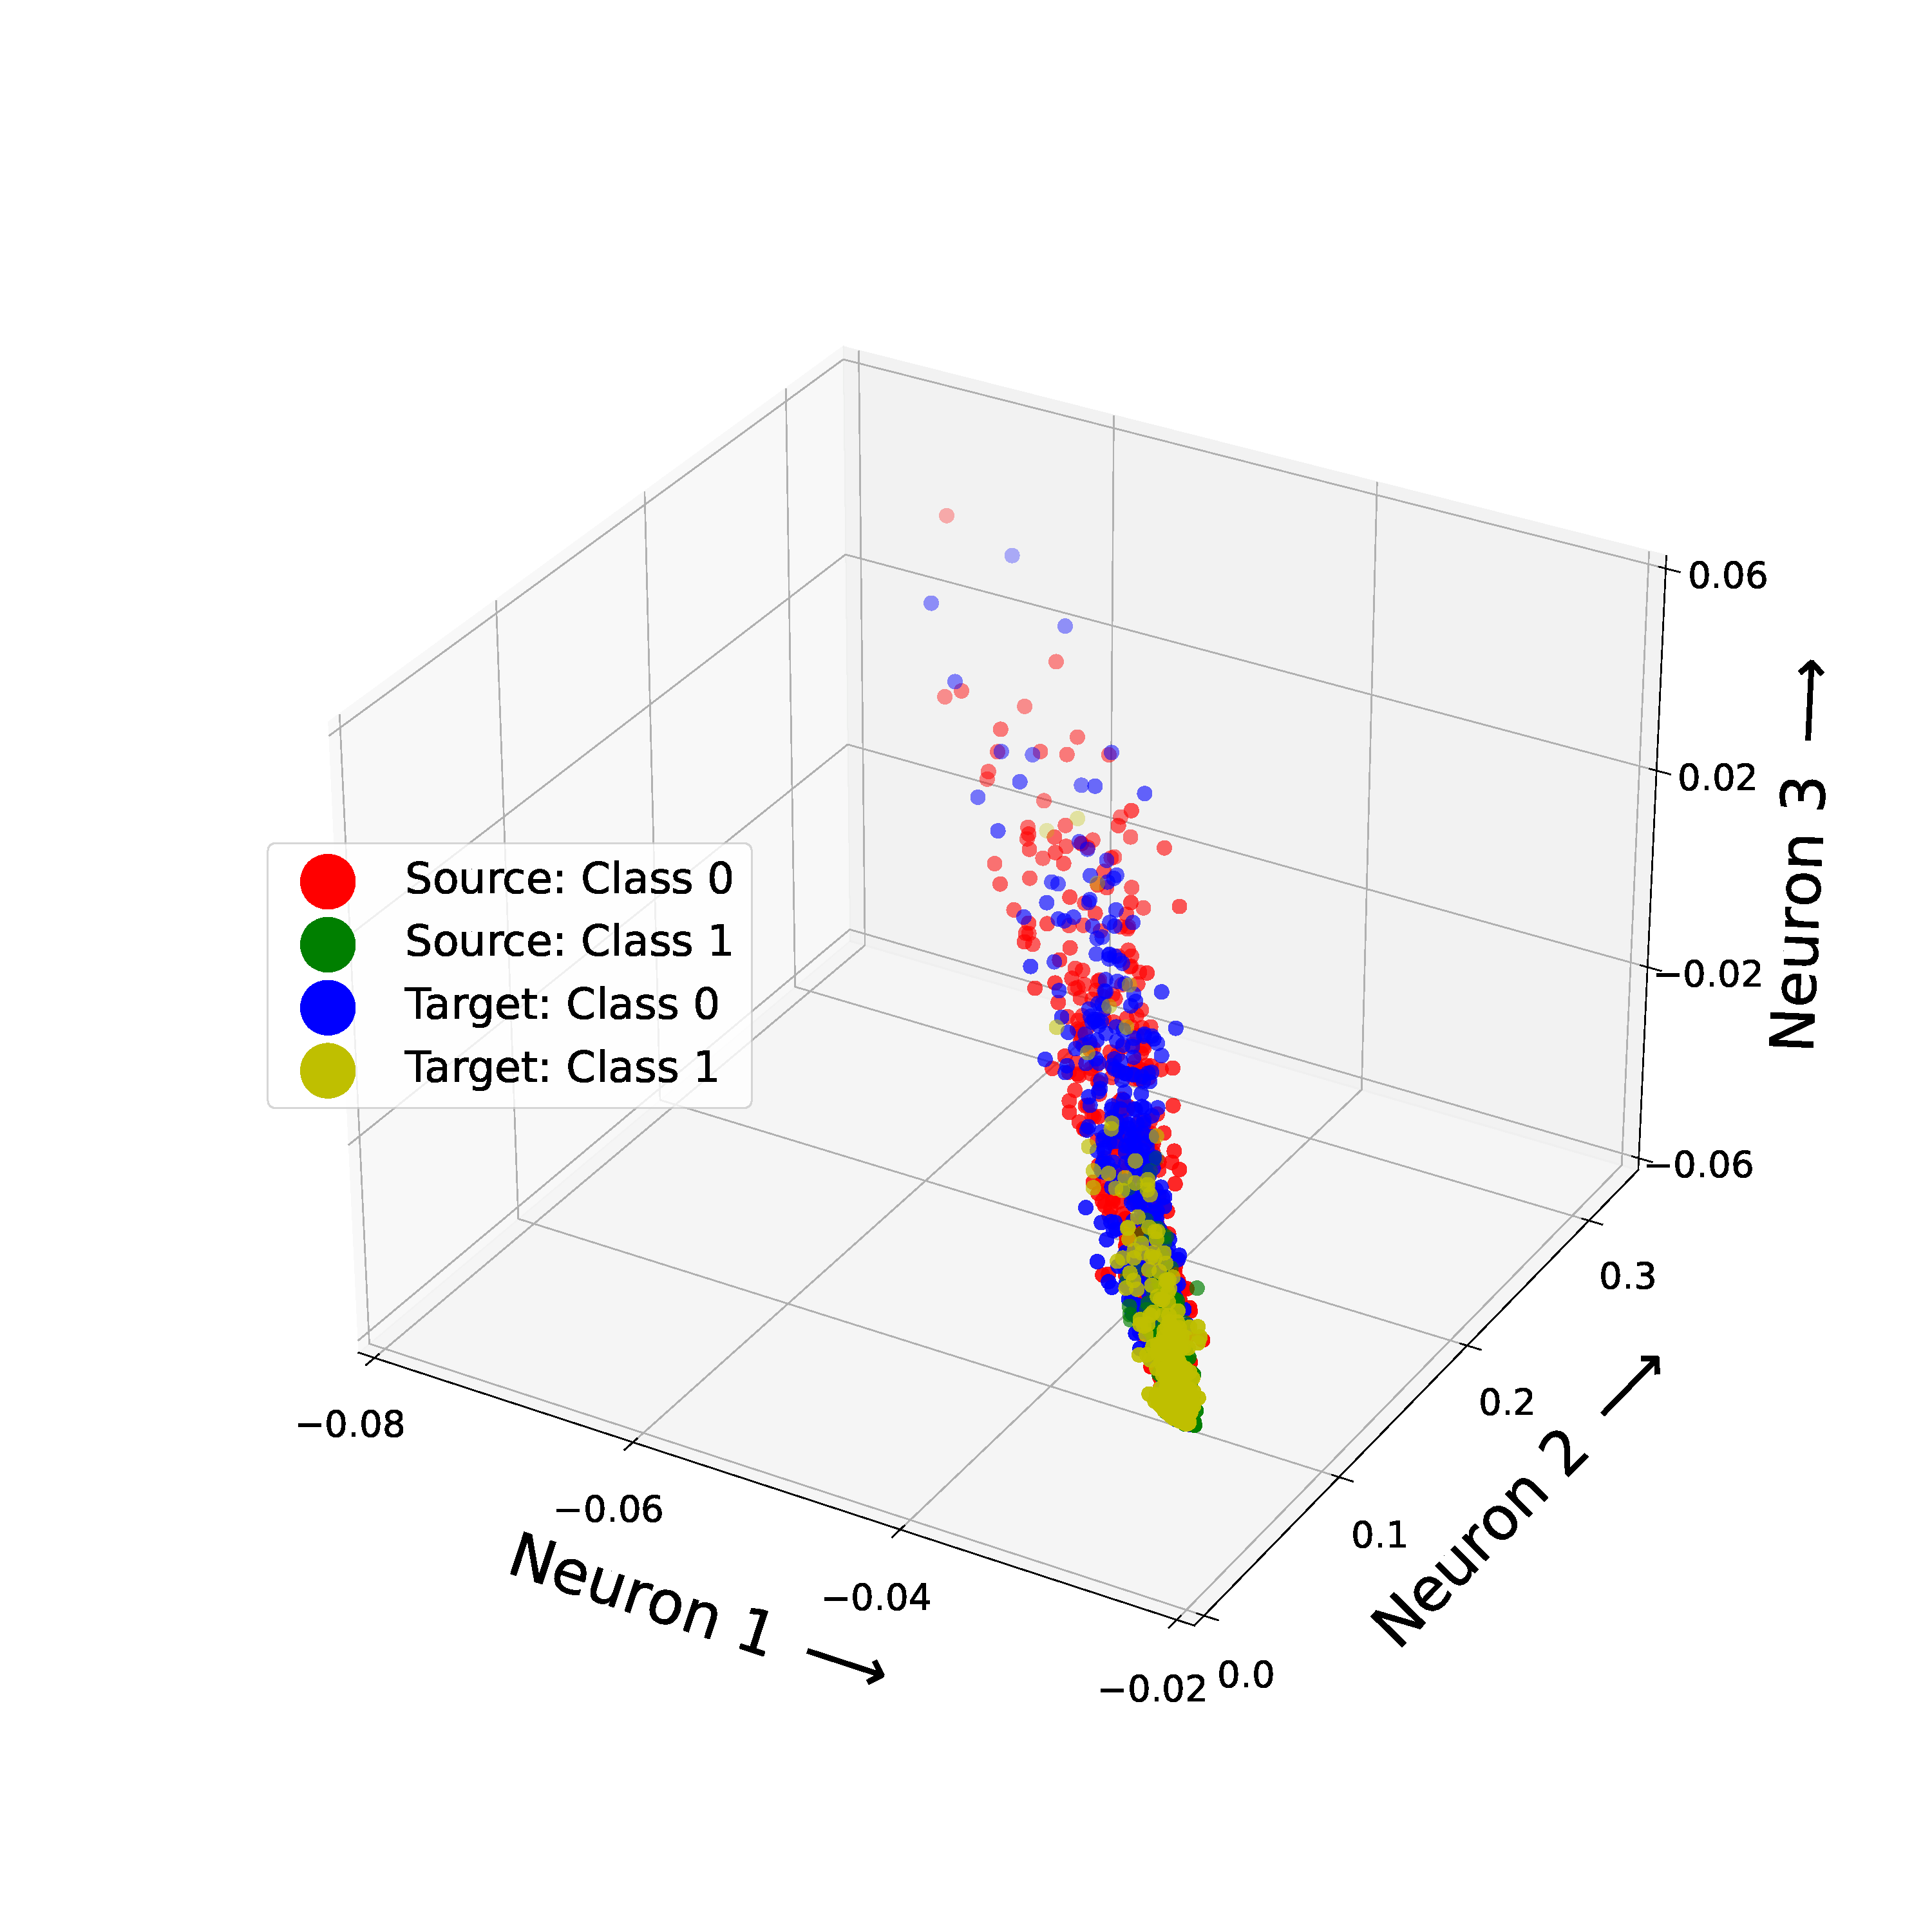
\includegraphics[width=.48\textwidth]{GAMMA_Influence_dummy_distribution/Dummy_distribution_8_GAMMA_20.pdf}
 

  \caption{Data distribution: Influence of GAMMA on Training, GAMMA = 0.05 (top), GAMMA = 0,4 (middle), GAMMA = 20 (bottom), Epoch = 0 (left) , Epoch = 8 (right)}
  \label{fig:point_cloud_mmd}
\end{figure}


\begin{figure}[H]
  \centering
  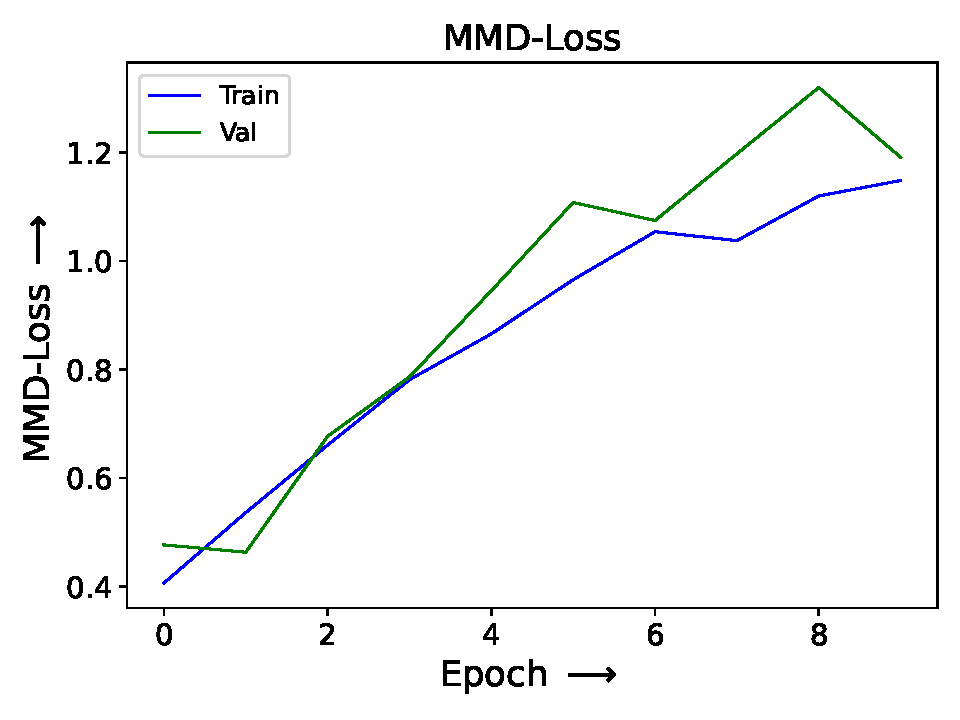
\includegraphics[width=.47\textwidth]{GAMMA_Influence_dummy_curve/MMD_Loss_GAMMA_0_001.pdf}
  \hspace{.3cm}
  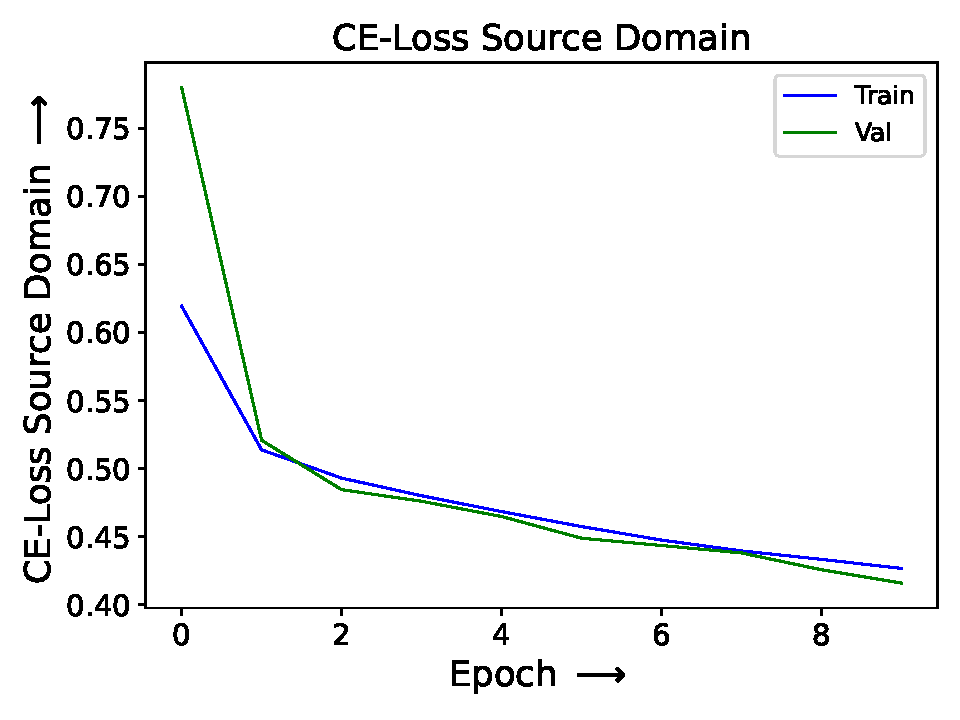
\includegraphics[width=.47\textwidth]{GAMMA_Influence_dummy_curve/CE_Loss_Source_Domain_GAMMA_0_001.pdf}

  \vspace{.1cm}

  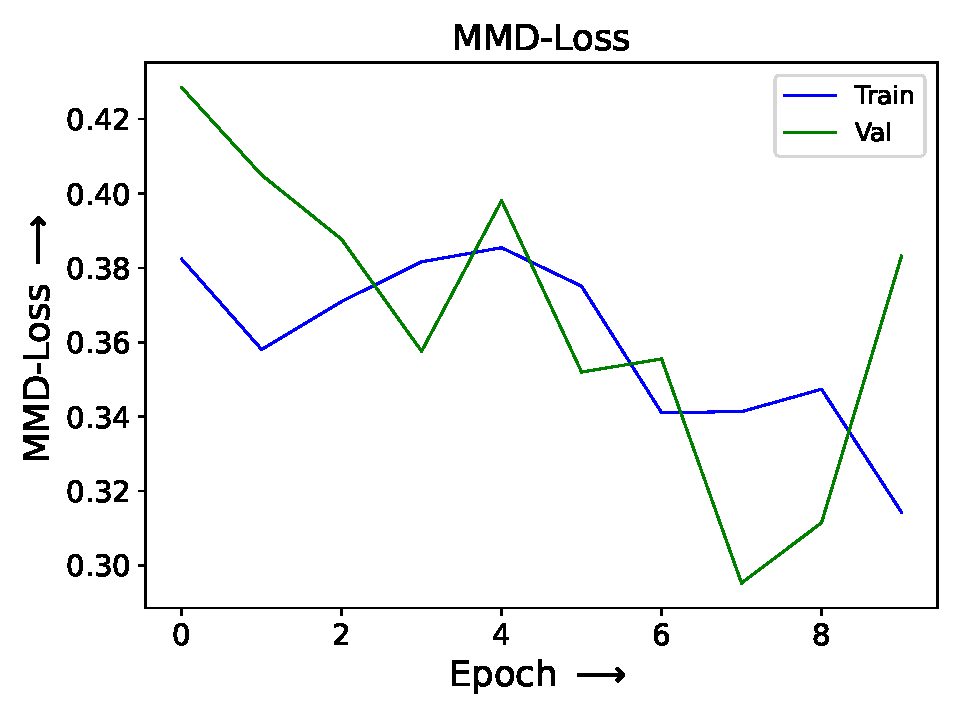
\includegraphics[width=.47\textwidth]{GAMMA_Influence_dummy_curve/MMD_Loss_GAMMA_0_1.pdf}
  \hspace{.3cm}
  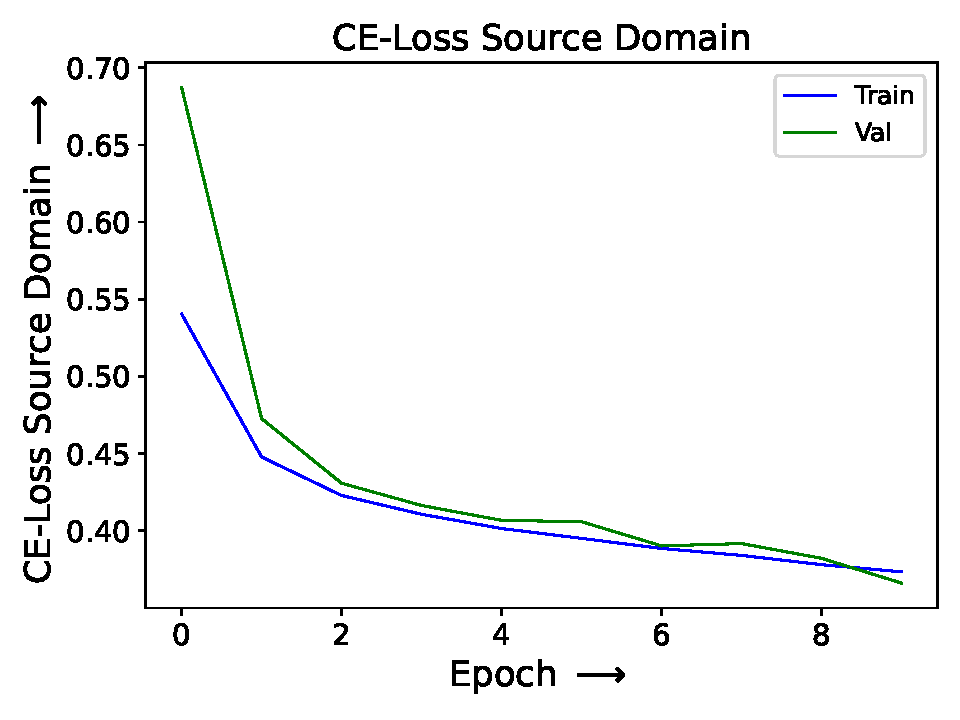
\includegraphics[width=.47\textwidth]{GAMMA_Influence_dummy_curve/CE_Loss_Source_Domain_GAMMA_0_1.pdf}

  \vspace{.1cm}

  \includegraphics[width=.47\textwidth]{GAMMA_Influence_dummy_curve/MMD_Loss_GAMMA_20.pdf}
  \hspace{.1cm}
  \includegraphics[width=.47\textwidth]{GAMMA_Influence_dummy_curve/CE_Loss_Source_Domain_GAMMA_20.pdf}

  \caption{MMD- and source CE-loss: Influence of GAMMA on Training: GAMMA = 0.001 (top), GAMMA = 0.1 (middle), GAMMA = 20 (bottom), Epoch 0 (left), Epoch 8 (right)}
  \label{fig:learning_curves_influence_mmd_feature_extractor}
\end{figure}

\subsection{Domain Adaptation Performance of a Labeled MMD-loss} \label{sec:Differences of labeled and unlabeled MMD loss}

In the unlabeled MMD-loss, the target labels are unknown. Therefore, the intra- and inter-class distance between source and target samples are minimized equally. As mentioned earlier, this increases the compactness but reduces the separability of classes in both domains. In the literature, some approaches, like the one proposed by Pandhare et al. \cite{Pandhare2021}, extend the unlabeled MMD-based model training with a distance-based optimization, which includes target labels. Usually, those approaches restrict the supervised training to the source domain. This section presents a novel labeled MMD-loss, which includes target labels and restricts the supervised training to the source domain. The domain discrepancy between source and target samples of similar and different classes is optimized separately. The labeled MMD-loss minimizes the intra-class and maximizes the inter-class discrepancy between the domains. This separate consideration of class distances allows a simultaneous improvement of the class separability and compactness. A weighted loss is applied, which combines the source CE-loss, the intra-class and the inter-class MMD-loss. This approach expects additional hyperparameters, which need to be defined beforehand. The hyperparameters GAMMA\_Intra\_Class and GAMMA\_Inter\_Class are used to balance the training scope of maximizing the inter-class distance and minimizing the intra-class distance as well as the source CE-loss:

\begin{equation}
\begin{split}
    \mbox{Total Loss} = & \mbox{GAMMA\_Intra\_Class}  \cdot \mbox{MMD\_Loss\_Intra\_Class} - \\
                              &\mbox{GAMMA\_Inter\_Class} \cdot \mbox{MMD\_Loss\_Inter\_Class} + \mbox{CE\_Loss}.
\end{split}
\end{equation}

The MMD-loss, which includes the target labels, is named "labeled MMD-loss" and otherwise "unlabeled MMD-loss". Again, fig. \ref{fig:point_cloud_labeled_unlabeled_mmd} visualizes the latent feature representations of the source and target samples in the FC2 layer. Throughout the training, the labeled MMD-loss can reduce the domain discrepancy while increasing the separability and compactness of the classes in both domains. In both domains, the distance between the classes is increased by a lot. The samples belonging to the same class are represented in a more distinct subset. The subsets corresponding to the same classes overlap more across the domains. These improvements, achieved by the labeled MMD-loss, simplify the classification problem. The labeled MMD-loss is interesting in a research aspect since it reveals the deficits of the unlabeled MMD-loss. Due to the lack of target labels, the unlabeled MMD-loss must be tuned carefully and mostly improves the compactness and domain discrepancy and not so much the separability. When the effect of the unlabeled MMD-loss becomes too strong, the separability between the classes is destroyed and the optimization ends up in the trivial solution, in which the latent feature representations of all samples collapse to a point- or needle-like subspace. In the labeled MMD-loss the domain discrepancy between samples of the same class is reduced and otherwise increased. This guarantees a simultaneous improvement of the compactness and separability. Therefore, the GAMMA choice is less sensible in the training and the MMD-loss influence can be increased. The optimization is less prone to get stuck in the just described trivial solution. This is also the reason, why in this experiment GAMMA\_Inter\_Class and GAMMA\_Intra\_Class could both be chosen to be 30. Just 20\% of labeled target labels were used in labeled MMD-loss.

\begin{figure}[htp]
  \centering
  \includegraphics[width=.44\textwidth]{labeled_vs_unlabeled_point_cloud/data_distribution_labeled_mmd_0.pdf}
  \hspace{.4cm}
  \includegraphics[width=.44\textwidth]{labeled_vs_unlabeled_point_cloud/data_distribution_labeled_mmd_8.pdf}

  \vspace{.1cm}

  \includegraphics[width=.44\textwidth]{labeled_vs_unlabeled_point_cloud/data_distribution_regular_mmd_0.pdf}
  \hspace{.4cm}
  \includegraphics[width=.44\textwidth]{labeled_vs_unlabeled_point_cloud/data_distribution_regular_mmd_8.pdf}
  
  \caption{Data Distribution: Labeled MMD (top) vs. unlabeled MMD (bottom): Epoch 0 (left) vs. Epoch 8 (right)}
  \label{fig:point_cloud_labeled_unlabeled_mmd}
\end{figure}

\subsection{Influence of Latent Feature Space Choice on the Domain Adaptation Performance}
\label{cnn_mmd_dummy}

This section analyzes the influence of applying the MMD-loss in different latent feature maps of the feature extractor and classifier. Inspired by Aljundi et al. \cite{Aljundi2016}, domain discrepancy reduction in the feature extractor layers is especially of interest. Two MMD-based approaches were evaluated, measuring the domain discrepancy in different neural network layers. Table \ref{tab:MMD_layer_choice_dummy} specifies the applied MMD-loss types in more detail.

\begin {table}[H]
\centering

\begin{tabular}{llllllll}
  \toprule
  Model          & Conv1 & Conv2 & Conv3 & Flatten & FC1 & FC2 \\
  \midrule
  
 
\vspace{.5cm}

 \parbox[t]{0mm}{\multirow{1}{*}{\rotatebox[origin=c]{90}{\thead{FC \\ MMD}}}} & - & - & - & \checkmark & \checkmark & \checkmark\\
 
\vspace{.5cm}

 \parbox[t]{0mm}{\multirow{1}{*}{\rotatebox[origin=c]{90}{\thead{FULL \\ MMD}}}} & \checkmark & \checkmark & \checkmark & \checkmark & \checkmark & \checkmark\\

  \bottomrule
\end{tabular}

\caption {MMD layer choice of presented models} \label{tab:MMD_layer_choice_dummy} 
\end {table}

The development of the source and target accuracy as well as the source CE- and MMD-loss throughout the model training are visualized in fig. \ref{fig:accuracy_cnn_and_no_cnn_mmd} and fig. \ref{fig:loss_cnn_and_no_cnn_mmd}. When including the CNN feature maps in the MMD-loss, higher source and target accuracy are achieved. Besides that, the losses, as well as the accuracy, converge faster and smoother. As Li et al. \cite{li2020} mentioned, the domain shift is not tackled sufficiently when reducing the domain discrepancy only in the final layers of the neural network. When estimating the MMD- and CE-loss solely in the final layers, it seems like the two contradicting training goals work against each other. The model training seems to get stuck in local minima, which leads to instabilities. The corresponding fluctuations can be seen in the training curves. Anyhow, one has to remember that calculating the FULL MMD-loss is quite expansive since the feature maps of the convolutional layers are complex and high-dimensional.

\begin{figure}[htp]
  \centering
  \includegraphics[width=.47\textwidth]{plots_CNN_MMD/Accuracy_Source_Domain_CNN_MMD.pdf}
  \hspace{.3cm}
  \includegraphics[width=.47\textwidth]{plots_CNN_MMD/Accuracy_Source_Domain_FC_MMD.pdf}

  \vspace{.1cm}

  \includegraphics[width=.47\textwidth]{plots_CNN_MMD/Accuracy_Target_Domain_CNN_MMD.pdf}
  \hspace{.3cm}
  \includegraphics[width=.47\textwidth]{plots_CNN_MMD/Accuracy_Target_Domain_FC_MMD.pdf}

  \caption{Source and Target Accuracy: MMD in CNN (left), MMD in FC (right)}
  \label{fig:accuracy_cnn_and_no_cnn_mmd}
\end{figure}

\begin{figure}[H]
  \centering
  \includegraphics[width=.47\textwidth]{plots_CNN_MMD/CE_Loss_Source_Domain_CNN_MMD.pdf}
  \hspace{.3cm}
  \includegraphics[width=.47\textwidth]{plots_CNN_MMD/CE_Loss_Source_Domain_FC_MMD.pdf}

  \vspace{.1cm}

  \includegraphics[width=.47\textwidth]{plots_CNN_MMD/MMD_Loss_CNN_MMD.pdf}
  \hspace{.1cm}
  \includegraphics[width=.48\textwidth]{plots_CNN_MMD/MMD_Loss_FC_MMD.pdf}

  \caption{MMD- and CE-Loss: MMD in CNN (left), MMD in FC (right)}
  \label{fig:loss_cnn_and_no_cnn_mmd}
\end{figure}

\section{Real-World Dataset}
In the following, the performance of models trained with different MMD-losses is evaluated on the real-world BSD dataset. This chapter's goal is to evaluate the benefits and problems of MMD-based domain adaptation for PHM of industrial machines. All presented models have the same architecture and optimization strategy but differ in the applied MMD-losses. The MMD-losses differ in their GAMMA and latent feature space choices. In the context of PHM of BSDs, the performance of MMD-based models is compared with a baseline model, which does not apply any MMD-loss during the training. Table \ref{tab:MMD_layer_choice}  specifies the latent feature spaces included in the different applied MMD-loss types:

\begin {table}[H]
\centering

\begin{tabular}{llllllll}
  \toprule
  Model          & Conv1 & Conv2 & Conv3 & Flatten & FC1 & FC2 \\
  \midrule
  
\vspace{.5cm}

 \parbox[t]{0mm}{\multirow{1}{*}{\rotatebox[origin=c]{90}{\thead{BASE- \\ LINE}}}} & - & - & - & - & - & -\\
 
\vspace{.5cm}

 \parbox[t]{0mm}{\multirow{1}{*}{\rotatebox[origin=c]{90}{\thead{FULL \\ MMD}}}} & \checkmark & \checkmark & - & \checkmark & \checkmark & \checkmark\\
 
\vspace{.5cm}

 \parbox[t]{0mm}{\multirow{1}{*}{\rotatebox[origin=c]{90}{\thead{FC \\ MMD}}}} & - & - & - & \checkmark & \checkmark & \checkmark\\
 
\vspace{.5cm}

 \parbox[t]{0mm}{\multirow{1}{*}{\rotatebox[origin=c]{90}{\thead{CNN \\ MMD}}}} & \checkmark & \checkmark & \checkmark & - & - & -\\

 
  \bottomrule
\end{tabular}

\caption {MMD layer choice of presented models} \label{tab:MMD_layer_choice} 
\end {table}

Similarly to the dummy dataset, the influence of the GAMMA and latent feature space choice in the applied MMD-losses on the PHM performance are examined in the chapters \ref{ch:Influence_GAMMA_real_dataset} and \ref{ch:Influence_Layer_real_dataset}. For several reasons, the previously presented labeled MMD-loss was excluded from this evaluation on the real-world BSD dataset. 
\begin{itemize}
    \item The labeled MMD-loss uses target labels, which in this evaluation no other MMD-loss type does. To achieve good comparability just models with equal prerequisites and data access during the training are considered in this evaluation.
    \item Optimization methods using target labels are impractical for real-world use. In domain adaptation tasks, neural networks are first trained on the source domain and afterward transferred to the target domain. If the optimization methods require target labels, one could train the neural networks directly on the target domain. Target labels prevent the easy model adaptation by solely including the unlabeled target dataset in the model training. Labeling a dataset is often done manually and can be quite time-consuming.
    \item The labeled MMD-loss expects additional hyperparameters. Finding those hyperparameters is more complicated and expects further experiments. The limited time in this thesis is also why the experiments on the real-world dataset are restricted to the unlabeled MMD-loss. 
\end{itemize}

In chapter \ref{ch:PHM_performance} the models are compared based on their performance on the real-world BSD dataset. In chapter \ref{ch:Performance_overview} the results from the dummy and real-world dataset are concluded once again. For the implementation of the presented models, PyTorch was used. All computations were performed on a Leibniz Supercomputing Centre7 compute node virtual machine with 20 Intel® Xeon® Gold 6148 vCPUs, one Nvidia® Tesla V100, 368 GB RAM, PyTorch v.1.4.0 and CUDA 10.1.


\subsection{Influence of GAMMA Choice on the PHM Performance}\label{ch:Influence_GAMMA_real_dataset}

In the following 3 models were trained with the FULL MMD-loss and different GAMMAs (0, 0.05, 1) on the  D:P mech./X signal for 100 epochs. Similarly to the dummy dataset, the MMD-based model training is very sensitive to the GAMMA choice. When GAMMA is chosen carefully, the domain discrepancy in the hidden layers can be reduced without decreasing the separability between the the source and target domain classes. Fig. \ref{fig:distribution_GAMMA_influence_real_data} shows the latent feature representations of the source and target domain samples in the FC2 layer. A GAMMA of 0.05 is a suitable choice for reducing the domain discrepancy while guaranteeing sufficient compactness and separability of the source and target classes. From the plots it is hard to compare the separability and compactness between different GAMMA choices. For a GAMMA of 0.05, the structure of the data distribution seems to be clearer and smoother. This raises the assumption that separating the classes in this scenario is easier. When picking a GAMMA of 0.05, especially class 1 seems to be more compact in both domains. When choosing a GAMMA of 1 the MMD-loss becomes too dominant. Noise and unimportant information are transferred between the domains. The MMD-loss reduces the distance between source and target samples from all classes. This destroys the class structure of the source and target domain, which makes the classification task impossible. In this case, the feature representations of all samples collapse to a small latent feature subspace.

\begin{figure}[H]
  \centering
  \includegraphics[width=.47\textwidth]{GAMMA_Influence_real_data/P_mech_X_data_distribution_0_GAMMA_0_0.pdf}
  \hspace{.4cm}
  \includegraphics[width=.47\textwidth]{GAMMA_Influence_real_data/P_mech_X_data_distribution_80_GAMMA_0_0.pdf}

  \vspace{.1cm}

  \includegraphics[width=.47\textwidth]{GAMMA_Influence_real_data/P_mech_X_data_distribution_0_GAMMA_0_05.pdf}
  \hspace{.4cm}
  \includegraphics[width=.47\textwidth]{GAMMA_Influence_real_data/P_mech_X_data_distribution_80_GAMMA_0_05.pdf}

  \vspace{.1cm}

  \includegraphics[width=.47\textwidth]{GAMMA_Influence_real_data/P_mech_X_data_distribution_0_GAMMA_1_0.pdf}
  \hspace{.4cm}
  \includegraphics[width=.47\textwidth]{GAMMA_Influence_real_data/P_mech_X_data_distribution_80_GAMMA_1_0.pdf}

  \vspace{.1cm}

  \caption{Data  distribution:  Influence  of  GAMMA  on  Training with D:P\_mech./X:  GAMMA  =  0  (top), GAMMA = 0.05 (middle), GAMMA = 1 (bottom), Epoch 0 (left), Epoch 100 (right)}
  \label{fig:distribution_GAMMA_influence_real_data}
\end{figure}


\subsection{Influence of Latent Feature Space Choice on the PHM Performance}\label{ch:Influence_Layer_real_dataset}
This section analyses the effects of different latent feature space choices on the MMD-based model training. All models were trained with a GAMMA of 1 on the D:I soll/X signal for 100 epochs. Each model training was repeated in five equally performed experiments. Fig. \ref{fig:target_accuracy_MMD_layer} shows the corresponding development of the target accuracy. When the MMD-loss is just applied in the FC layers, the training collapses in two of the five experiments (row 3 $\&$ 5). In the other three cases, the accuracy has a slight tendency to decrease during the training. The CNN MMD-based model training shows worse reproducibility throughout the five experiments than the FULL MMD-based model training. Often, the fluctuations on the validation data are not reduced properly throughout the training (row 1 $\&$ 4 $\&$ 5). Especially towards the end of the training, the FULL MMD-based model training seems to be more stable. Anyhow, minor fluctuations are also observable for the FULL MMD-based model training (row 3 $\&$ 4). In this thesis, the final model is picked based on its performance on the validation dataset of the target domain. In real-world scenarios, the target labels are often unknown. Often, the model at the end of the training is picked as the final one. When the model performance decreases or fluctuates throughout the training, the best possible model will not be found. For this reason, a stable model training should not be underestimated. A more detailed description of how the final models are picked is given in chapter \ref{ch:PHM_performance}. 

\begin{figure}[H]
  \centering

  \includegraphics[width=.32\textwidth]{MMD_LAYER_influence_real_data/CNN_MMD/Accuracy_Target_Domain_1.pdf}
  \hspace{.1cm}
  \includegraphics[width=.32\textwidth]{MMD_LAYER_influence_real_data/FC_MMD/Accuracy_Target_Domain_1.pdf}
  \hspace{.1cm}
  \includegraphics[width=.32\textwidth]{MMD_LAYER_influence_real_data/FULL_MMD/Accuracy_Target_Domain_1.pdf}

  \vspace{.3cm}

  \includegraphics[width=.32\textwidth]{MMD_LAYER_influence_real_data/CNN_MMD/Accuracy_Target_Domain_2.pdf}
  \hspace{.1cm}
  \includegraphics[width=.32\textwidth]{MMD_LAYER_influence_real_data/FC_MMD/Accuracy_Target_Domain_2.pdf}
  \hspace{.1cm}
  \includegraphics[width=.32\textwidth]{MMD_LAYER_influence_real_data/FULL_MMD/Accuracy_Target_Domain_2.pdf}

  \vspace{.3cm}

  \includegraphics[width=.32\textwidth]{MMD_LAYER_influence_real_data/CNN_MMD/Accuracy_Target_Domain_3.pdf}
  \hspace{.1cm}
  \includegraphics[width=.32\textwidth]{MMD_LAYER_influence_real_data/FC_MMD/Accuracy_Target_Domain_3.pdf}
  \hspace{.1cm}
  \includegraphics[width=.32\textwidth]{MMD_LAYER_influence_real_data/FULL_MMD/Accuracy_Target_Domain_3.pdf}
  
    \vspace{.3cm}

  \includegraphics[width=.32\textwidth]{MMD_LAYER_influence_real_data/CNN_MMD/Accuracy_Target_Domain_4.pdf}
  \hspace{.1cm}
  \includegraphics[width=.32\textwidth]{MMD_LAYER_influence_real_data/FC_MMD/Accuracy_Target_Domain_4.pdf}
  \hspace{.1cm}
  \includegraphics[width=.32\textwidth]{MMD_LAYER_influence_real_data/FULL_MMD/Accuracy_Target_Domain_4.pdf}
  
    \vspace{.3cm}
    
  \includegraphics[width=.32\textwidth]{MMD_LAYER_influence_real_data/CNN_MMD/Accuracy_Target_Domain_5.pdf}
  \hspace{.1cm}
  \includegraphics[width=.32\textwidth]{MMD_LAYER_influence_real_data/FC_MMD/Accuracy_Target_Domain_5.pdf}
  \hspace{.1cm}
  \includegraphics[width=.32\textwidth]{MMD_LAYER_influence_real_data/FULL_MMD/Accuracy_Target_Domain_5.pdf}


  \caption{Target Accuracy: Influence of MMD layer Choice on Training: CNN MMD (left), FC MMD (middle), FULL MMD (right)}
  \label{fig:target_accuracy_MMD_layer}
\end{figure}


\section{Overal PHM Performance}\label{ch:PHM_performance}
By evaluating models trained with different MMD-loss types, the utility and applicability of MMD-based model training for real-world PHM tasks are evaluated in this chapter. In the first step, all of the 49 signals were evaluated for their suitability in PHM systems. For this, models were trained on these signals without applying any MMD-loss. Based on the performance of these models, seven promising signals were picked for further testing. In a second step, an MMD-based model training was applied to these 7 signals. Models were optimized with FULL MMD-, FC MMD- and CNN MMD-losses and three different GAMMAs (0.05 $\&$ 0.5 $\&$ 1). All nine MMD-based model training (all combinations of MMD types and GAMMAs) and the baseline model training, which does not apply any MMD-loss, were repeated in five equally performed experiments on all seven signals. In each epoch during the MMD-based model training, the models were evaluated based on the balanced accuracy on the target domain validation dataset. Throughout the training, the best-performing model was stored. The different MMD-loss types were compared based on the performance of those stored models on the unseen target domain test dataset. The average accuracy from all five equally trained models on the target domain test dataset is shown in table \ref{tab:Mean_Accuracy}. For four of the seven signals, the FULL MMD and the other three the CNN MMD models perform best. The FC MMD models never outperform the other MMD-based models. Compared to the baseline model, the MMD-based models can increase the accuracy by up to 10.18$\%$. Table \ref{tab:Variance_Accuracy} shows the corresponding variance to the averaged accuracy in table \ref{tab:Mean_Accuracy}. The best-performing models usually show low to average variances. A low variance verifies a high degree of reproducibility throughout the repeated experiments. This demonstrates the meaningfulness of the results and proves the applicability and utility of MMD-losses for reducing the domain discrepancy in PHM tasks. Table \ref{tab:Average_Variance_Accuracy} shows the average variance over the 105 MMD-based models (7 signals, 3 GAMMAs, 5 experiments) and the 35 baseline models (7 signals, 5 experiments). From the MMD-based models, the FULL MMD models have the lowest and the FC MMD models have the highest average accuracy variance. This shows that the FULL MMD models have the highest consistency throughout the executed experiments, which were performed with varying GAMMAs on different signals. The FULL MMD models seem more robust and less sensible to GAMMA and signal choices. As mentioned in the results of the dummy dataset, a reason for the sensitivity of the FC MMD model training might be the contradicting training goals when evaluating the MMD- as well as the source CE-loss just in the FC layers. The shifting focus on different training goals during the training might lead to instabilities. In such cases, the training is more prone to getting stuck in local minima.
\begin{comment}
Windowing functions split the recorded data in shorter sequences. The generated windows should capture the degradation related patterns of the vibration signals. For this reason, the windows should be adapted according to the consistency and periodicity of the data. In this thesis a window size of 1024 was chosen. The windowing requirements are different for the different machine excitements (constant speed excitement, direction change excitement and sweep excitement). The windows are too short to capture one whole period of of forward and backward motion in the data recorded during constant speed machine excitement. The data can be separated in phases of constant speed and direction change, which each contains roughly 1000 datapoints. The windows are of equal size as the described phases in the data. Since the windows are not synchronized with those phases, they overlap to a large extent but do not cover them perfectly. The windows are big enough to capture several periods of forward and backward movements in data recorded during direction change excitement. When exciting the machine with a sweep signal the PHM system should better process the whole corresponding vibration signal. It is important to capture the changing frequencies and amplitudes during the complete sweep excitement. The best PHM results were achieved on data recorded during constant speed and  direction change excitement of the machine. This shows that the windowing did not work very well on the data recorded during sweep excitement. Generally, when choosing the window size, there is a trade-off between the window size and the number of windows generated from the data. Both extremes (few big windows and numerous small windows) might lead to problems during the training. The PHM results can probably be improved by an intelligent and adaptive preprocessing to generate suitable and synchronized data windows. Azamfat et al \cite{AZAMFAR2020103932} present such an approach. They apply a constant excitement to the machine and separate the data BSD phases of constant velocity direction change movement. The PHM system just relies on the data recorded during BSD constant velocity. The signals D:I\_ist/X (actual electrical power), D:I\_soll/X (target electrical power) and D:P\_mech./X (mechanical power) coming from the controller show high potential for the PHM task. The most suitable accelerometer installation is the one on the BSD nut. Pandahare et al \cite{Pandhare2021} discovered similar results. Often in real operational scenarios such an installation is impractical \cite{Pandhare2021}. Alternatively to the BSD nut position, this thesis shows, that the top LGS achieves better PHM results than the bottom one.
\end{comment}


\begin{sidewaystable}
\begin {table}[H]
\centering
\begin{tabular}{llllllllll}
  \toprule
  Model          & GAMMA    & D:I\_ist/X & D:I\_soll/X & D:P\_mech./X & C:z\_top & C:z\_nut & D:x\_nut & D:z\_top \\
  \midrule
  
  \vspace{1cm}
  
    \thead{BASE- \\ LINE}  & -      & 70.08 & 75.62 & 74.7 & 69.14 & 57.4 & 58.74 & 57.88\\


 
                            & 0.05   & 71.56 & 75.42 & \textbf{78.96} & 72.36 & 58.10 & 49.52 & \textbf{62,64}\\
    \thead{FULL \\ MMD}     & 0.5    & 73.78 & 74.84 & 52.78 & \textbf{75.92} & \textbf{64.76} & 50.52 & 49,94\\
    
    \vspace{1cm}
    
                            & 1      & 72.98 & 75.18 & 49.80 & 74.12 & 57.02 & 50.62 & 50.52\\


                            & 0.05   & 73.60 & 76.38 & 74.98 & 71.36 & 57.48 & 52.44 & 61.3\\
    \thead{FC \\ MMD}       & 0.5    & 70.74 & 74.86 & 72.62 & 69.32 & 59.76 & 50.12 & 53.22\\
    
    \vspace{1cm}
    
                            & 1      & 73.42 & 65.46 & 76.96 & 62.34 & 58.86 & 50.92 & 53.96\\

                            & 0.05   & 71.62 & \textbf{76.44} & 51.80 & 73.20 & 59.30 & 58.04 & 53.82\\
    \thead{CNN \\ MMD}      & 0.5    & \textbf{73.90} & 75.86 & 51.58 & 72.28 & 55.76 & 68.04 & 51.72\\
                            & 1      & 73.80 & 73.82 & 51.12 & 72.18 & 54.28 & \textbf{68.92} & 51.28\\
 \addlinespace
 \hline
 \thead{MMD\\GAIN:} &  & +3.82 & +0.82 & +4.26 & +6.78 & +7.36 & +10.18 & +4.76\\
 
  \bottomrule
\end{tabular}
\caption {Mean target test accuracy (\%)} \label{tab:Mean_Accuracy} 
\end {table}
\end{sidewaystable}

\begin{sidewaystable}
\begin {table}[H]
\centering
\begin{tabular}{llllllllll}
  \toprule
  Model          & GAMMA    & D:I\_ist/X & D:I\_soll/X & D:P\_mech./X & C:z\_top & C:z\_nut & D:x\_nut & D:z\_top  \\
  \midrule

    \vspace{1cm}

    \thead{BASE- \\ LINE}   & -      & 2.07 & 0.27 & 2.20 & 2.55 & 1.11 & 1.04 & 1.22\\
 
                            & 0.05   & 1.06 & 0.74 & \textbf{1.79} & 1.80 & 2.04 & 1.39 & \textbf{2.48}\\
    \thead{FULL \\ MMD}     & 0.5    & 0.72 & 1.44 & 3.33 & \textbf{1.72} & \textbf{1.42} & 1.23 & 1.02\\
    
    \vspace{1cm}  
    
                            & 1      & 0.76 & 0.81 & 0.87 & 6.06 & 5.57 & 0.96 & 0.79\\



                            & 0.05   & 1.96 & 0.61 & 1.86 & 1.82 & 1.63 & 3.86 & 1.60\\
    \thead{FC \\ MMD}       & 0.5    & 1.34 & 0.72 & 11.06 & 6.42 & 2.28 & 0.45 & 3.14\\
    
    \vspace{1cm}
    
                            & 1      & 0.96 & 12.01 & 5.46 & 8.18 & 2.13 & 0.93 & 2.70\\
                            & 0.05   & 2.13 & \textbf{0.53} & 2.39 & 1.12 & 4.01 & 4.18 & 7.26\\
    \thead{CNN \\ MMD}      & 0.5    & \textbf{0.25} & 1.57 & 1.08 & 1.22 & 3.27 & 3.51 & 3.22\\
                            & 1      & 0.51 & 1.25 & 2.02 & 2.51 & 4.54 & \textbf{2.54} & 2.34\\
  \bottomrule
\end{tabular}
\caption {Standard deviation target test accuracy (\%)} \label{tab:Variance_Accuracy} 
\end {table}
\end{sidewaystable}


\begin {table}[H]
\centering
\begin{tabular}{lllll}
  \toprule
  Model & BASE-LINE & FULL MMD & FC MMD & CNN MMD\\
  \midrule
  AVG VARIANCE & 1.50 & 1.81 & 3.39 & 2.45\\
  \bottomrule
\end{tabular}
\caption {Average standard deviation target test accuracy (\%)} \label{tab:Average_Variance_Accuracy} 
\end {table}

\section{Conclusion of the Experimental Results}\label{ch:Performance_overview}
In this chapter, the findings from the experiments on the dummy and real-world datasets are summarized. Variations in the underlying functionality and mechanism of the MMD-loss types became especially visible in the experiments on the dummy dataset. Performance differences between the MMD-loss types were evaluated on the real-world dataset. A novel labeled MMD-loss was developed, which considers the source and target labels. When applying the labeled MMD-loss, the domain discrepancy is reduced between samples of the same class and increased between those of different classes. This guarantees an improved compactness and separability in all classes while reducing the domain discrepancy. The experiments with the labeled MMD-loss on the dummy dataset highlighted the deficits of the unlabeled MMD-loss. Since the unlabeled MMD loss has no access to the target labels, class-specific properties like the compactness and separability can not be optimized for the target domain. The unlabeled MMD-loss reduces the domain discrepancy between all samples without considering their class labels. If the unlabeled MMD-loss becomes too dominant, the separability of the classes is reduced and the data structure is destroyed. In this case, the latent feature space representations of all samples collapse to a point- or needle-like subspace. This makes the classification more challenging. For this reason, the GAMMA choice is highly relevant and has to be picked carefully and individually for each signal. The experiments on the real-world dataset showed, that the MMD-losses, applied in early CNN layers, reduce the domain discrepancy more efficiently than those restricted to the FC layers. This greater efficiency is mainly reflected in the overall model performance and the increased training stability. In the experiments, the model optimization showed less fluctuation and higher reproducibility. When applying an MMD-loss in the feature extractor layers, the training is less sensitive to specific GAMMA and signal choices. 
\chapter{Conclusion}\label{chapter:conclusion}
In this thesis a deep learning-based PHM system for BSDs was successfully extended with a domain adaption module. A novel way of reducing the domain discrepancy in the network's feature extractor was developed. Applying the MMD-loss in the layers of the CNN and classifier reduces the model's domain discrepancy more efficiently than the more traditional approaches, which just apply the MMD-loss in the task specific layers. This greater efficiency is mainly reflected in the overall performance and the increased stability during the training. A novel labeled MMD-loss, which considers the source and target labels, revealed the main deficit of the unlabeled MMD-loss. Oftentimes, the unlabeled MMD-loss can not improve the separability equally good as the compactness and domain discrepancy throughout the training. The GAMMA choice is highly relevant for the PHM performance and has to be picked individually for each signal. An imperfect GAMMA choice reduces the separability and leads to a trivial optimization solution, where the feature representation of all samples collapse at a small subset. 

\chapter{Outlook}
In future work, the dataloader could be extended with more sophisticated pre-processing steps. Wavelet transforms or FFTs, could be applied to the raw input data to feed more expressive data to the neural network. In the literature, it is quite common to include such steps \cite{Li2018} \cite{Kang2020} \cite{Zhang2017}. Investigating to what extent such methods could increase the PHM performance would be very interesting.

In the experiments of this thesis, the best PHM results were achieved with the direction change excitation and the worst were accomplished with the sweep excitation. The excitation of the machine and, thus, the signals showing the machine’s reaction differ fundamentally in their periodicity and constant BSD velocity phases. Even though the pre-processing effort might increase, it should be investigated how the adaptation and synchronization of the data windowing to the periodicity and constant BSD velocity phases of the machine's excitation can increase the PHM performance. Azamfar et al. \cite{AZAMFAR2020103932} mention that the amplitude and frequency variations during a phase of constant BSD velocity deliver more expressive information about the machine's degradation. In the literature, regime separation strategies, which split the data into physical meaningful sequences, are widespread \cite{AZAMFAR2020103932} \cite{Pandhare2021}.

Furthermore, new domain shift problems could be generated to test the proposed PHM system. Training and testing the model on differently degraded LGSs would be a realistic and challenging task.

Moreover, the application of the labeled MMD-loss on real-world data is worth being further investigated. A labeled MMD-loss that only uses a small amount of target labels might be beneficial for some PHM tasks. If labeling some target samples is acceptable, a more effective adaptation of PHM systems might be achievable with that MMD-loss type.

There are several other approaches that should be considered for monitoring the health condition of BSDs. Recently, GANs became more popular for PHM of industrial machines \cite{Zhang2019}. The adversarial training of those models is promising for the extraction of domain-invariant features. However, the development and training of GANS is more complex. Especially when applying such models to noisy and disturbed real-world data, this might lead to training instabilities \cite{Zhang2019}. 



\begin{comment}
%%% example of different requirements to capture information from the signals of different excitation %%%
The window size was set to 1024 and the windows were not synchronized with the data. In the direction change excitation signals, the windows could capture several periods of direction change movements. In the constant speed excitation signals, the windows were generally large enough to capture all data points from the direction change phase and the constant velocity phase but the windows were not properly synchronized with those. The windows could not cover all corresponding data points in the sweep excitation signals.
\end{comment}


\begin{comment}
Also the preprocessing of the recorded machine signals could be improved. In this thesis a simple windowing function was used to separate the data in shorter sequences. Generally, the generated windows should capture the degradation related patterns of the vibration signals. For this reason, the windows should be adjusted to the consistency and periodicity of the data. The windowing requirements differ for the machine excitements (constant speed excitement, direction change excitement and sweep excitement). Generally, when choosing the window size, there is a trade-off between the window size and the number of windows generated from the data. Both extremes (few big windows and numerous small windows) might lead to problems during the training. The PHM results might be improved by applying an adaptive preprocessing to generate data windows of suitable length, which are well synchronized with the data. Lastly, also the potential performance gains due to the combination of several signals could be investigated in more detail.
\end{comment}
% TODO: add more chapters here



\appendix{}

% TODO: appendix chapter
\chapter{General Addenda}



\begin{center}
\begin{longtable}{c c c c} 
 \toprule
 Signal & Sensor & Frequency & Samples \\ [0.5ex] 
 \midrule
 C:s ist/X & TNC Scope & 10 kHz & 75000 \\ 

 C:s soll/X & TNC Scope & 10 kHz & 75000 \\ 

 C:s diff/X & TNC Scope & 10 kHz & 75000 \\ 

 C:v (n ist)/X & TNC Scope & 10 kHz & 75000 \\ 

 C:v (n soll)/X& TNC Scope & 10 kHz & 75000 \\ 

 C:P mech./X & TNC Scope & 10 kHz & 75000 \\ 

 C:Pos. Diff./X & TNC Scope & 10 kHz & 75000 \\ 

 C:I ist/X & TNC Scope & 10 kHz & 75000 \\ 

 C:I soll/X & TNC Scope & 10 kHz & 75000 \\ 

 C:x bottom & Acc & 10 kHz & 75000 \\ 

 C:y bottom & Acc & 10 kHz & 75000 \\ 

 C:z bottom & Acc & 10 kHz & 75000 \\ 

 C:x nut & Acc & 10 kHz & 75000 \\ 

 C:y nut & Acc & 10 kHz & 75000 \\ 

 C:z nut & Acc & 10 kHz & 75000 \\ 

 C:x top & Acc & 10 kHz & 75000 \\ 

 C:y top & Acc & 10 kHz & 75000 \\ 

 C:z top & Acc & 10 kHz & 75000 \\ 

 D:s ist/X & TNC Scope & 10 kHz & 75000 \\

 D:s soll/X & TNC Scope & 10 kHz & 75000 \\ 

 D:s diff/X & TNC Scope & 10 kHz & 75000 \\ 

 D:v (n ist)/X & TNC Scope & 10 kHz & 75000 \\ 

 D:v (n soll)/X & TNC Scope & 10 kHz & 75000 \\ 

 D:P mech./X & TNC Scope & 10 kHz & 75000 \\ 
 
 D:Pos. Diff./X & TNC Scope & 10 kHz & 75000 \\ 

 D:I ist/X & TNC Scope & 10 kHz & 75000 \\ 

 D:I soll/X & TNC Scope & 10 kHz & 75000 \\ 

 D:x bottom & Acc & 10 kHz & 75000 \\ 

 D:y bottom & Acc & 10 kHz & 75000 \\ 

 D:z bottom & Acc & 10 kHz & 75000 \\ 

 D:x nut & Acc & 10 kHz & 75000 \\ 

 D:y nut & Acc & 10 kHz & 75000 \\ 

 D:z nut & Acc & 10 kHz & 75000 \\ 

 D:x top & Acc & 10 kHz & 75000 \\

 D:y top & Acc & 10 kHz & 75000 \\ 

 D:z top & Acc & 10 kHz & 75000 \\ 

 S:x bottom & Acc & 10 kHz & 153601 \\ 

 S:y bottom & Acc & 10 kHz & 153601 \\ 

 S:z bottom & Acc & 10 kHz & 153601 \\ 

 S:x nut & Acc & 10 kHz & 153601 \\ 

 S:y nut & Acc & 10 kHz & 153601 \\ 

 S:z nut & Acc & 10 kHz & 153601 \\ 

 S:x top & Acc & 10 kHz & 153601 \\ 

 S:y top & Acc & 10 kHz & 153601 \\ 
 
 S:z top & Acc & 10 kHz & 153601 \\ 
 
 S:Nominal rotational speed & TNC opt & 1 kHz & 16384 \\
 
 S:Actual rotational speed & TNC opt & 1 kHz & 16384 \\ 
 
 S:Actual position of the position encoder(dy/dt) & TNC opt & 1 kHz & 16384 \\ 
 S:Actual position of the motor encoder(dy/dt)  & TNC opt & 1 kHz & 16384  \\ [1ex] 
 \bottomrule
\caption {Description of recorded signals}
\label {tab:description_of_the_49_recorded_features}
\end{longtable}
\end{center}


\begin{comment}
    

If there are several additions you want to add, but they do not fit into the thesis itself, they belong here.


\section{Generative Adversarial Network}
Generative Adversarial Networks (GANs) are generative models which recently became more and more popular. Generative models can capture the data distribution of samples seen during training. Such models are able to synthetically generate new instances belonging to the train data distribution without actually being part of that dataset. They can be used in an unsupervised or a supervised manner, which means, they are able to perform feature learning/extraction and classification. GANs include two different models. A generator network (G) learns the data distribution of the training data. Given noise, the generator network produces synthetic data. The discriminator (D) model tries to classify the seen data between synthetic generator's output and true data. D(x) represents the probability that x comes from the real data rather than from the generator. The optimization process of GANs is a minimax game process:
\begin{equation}
    \min_{G} \max_{D} \mathbb{E}_{x \sim P_{r}} [log(D(x))] + \mathbb{E}_{\tilde{x} \sim P_{g}}[log(1-D(\tilde{x}))],
    \label{eq:GAN_Training}
\end{equation}
where $P_{r}$ is the distribution of the real input data and $P_{g}$ is the data distribution from the generator's output, which is defined by  $\tilde{x}  \sim G(z)$. A Uniform or Gaussian distribution can be used to sample the noise $z \sim p(z)$. In theory the generator should be learned such that eq. \ref{eq:GAN_Training} is minimized. This is achieved if the discriminator falsely classifies the real and the synthetic generator's outputs ($D(x) \sim 0$ and $D(\tilde{x}) \sim 1$). On the other hand, the discriminator should be learned such that eq. \ref{eq:GAN_Training} is maximized, which means that the discriminator correctly labels all samples ($D(x) \sim 1$ and $D(\tilde{x}) \sim 0$). The discriminator and generator are optimized in an alternating procedure \cite{Goodfellow2014}. In order to prevent overfitting, one should alternate between k steps of optimizing D and one step of optimizing G \cite{Goodfellow2014}. The optimization of GANs proposed by Goodfellow et al \cite{Goodfellow2014} is described in the Algorithm \ref{alg.GAN_optimization}.

\begin{algorithm}
\caption{Iterative optimization of GANs}\label{alg:cap}
\begin{algorithmic}
\While{$\textrm{train iterations} < \textrm{max iterations}$}
    \While{$\textrm{discriminator optimization steps} < \textrm{k}$}
        \State $\cdot$ Sample m noise samples ${\pmb{z}^{(1)}, . . . , \pmb{z}^{(m)}}$ from noise distribution $p(\pmb{z})$
        \State $\cdot$ Sample m noise samples ${\pmb{x}^{(1)}, . . . , \pmb{x}^{(m)}}$ from real data distribution $P_{r}$
        \State $\cdot$ Update the discriminator by ascending its stochastic gradient:
        \begin{equation*}
            \nabla_{\theta_{d}} \frac{1}{m} \sum_{i=1}^{m} [log(D(\pmb{x}^{(i)})) + log(1-D(G(\pmb{z}^{(i)})))].
        \end{equation*}
    \EndWhile
    \State $\cdot$ Sample m noise samples ${\pmb{z}^{(1)}, . . . , \pmb{z}^{(m)}}$ from noise distribution $p(\pmb{z})$
    \State $\cdot$ Update the generator by descending its stochastic gradient:
    \begin{equation*}
        \nabla_{\theta_{g}} \frac{1}{m} \sum_{i=1}^{m} log(1-D(G(\pmb{z}^{(i)}))).
    \end{equation*}
\EndWhile
\label{alg.GAN_optimization}
\end{algorithmic}
\end{algorithm}

Besides that, eq. \ref{eq:GAN_Training} does not deliver sufficient gradients for gradient-based optimization of GANs. The problem is, that in early stages the generator performance is poor, such that the discriminator rejects all synthetic generator's outputs, which prevents the generator training. Instead, the generator can be trained to maximize $D(\tilde{x})$. This objective achieves the same results as eq. \ref{eq:GAN_Training} but delivers stronger gradients in early learning stages \cite{Goodfellow2014}. Fig \ref{fig:GAN_training_vizualization} shows the alternating optimization of the discriminator and generator. 

\begin{figure}[H]
  \centering
  \includegraphics[width=1\textwidth]{GAN_training_vizualization.pdf}
  \caption{When optimizing GANs the discriminator and generator are optimized simultaneously in an alternating procedure. The blue dashed line represents the discriminator probability of x belonging to the real data distribution rather than being created by the generator. The black dashed line represents the generative distribution and the green solid line the real data distribution. (a) shows a generator, discriminator pair near convergence, (b) shows the GAN performance after passing the inner loop of Algorithm \ref{alg.GAN_optimization}, which optimizes the discriminator. (c) shows the GAN performance after passing through one whole training loop in Algorithm \ref{alg.GAN_optimization}. Now the generator and the discriminator are both optimized. (d) shows the GAN performance after several training iterations. The generator completely learned the real data distribution, such that the discriminator is not able to separate between samples from the real data distribution and synthetic generator outputs \cite{Goodfellow2014}.}
  \label{fig:GAN_training_vizualization}
\end{figure}




\section{Other Related Work}
In the following sections several works in the domain adaption and PHM context are presented, which are mentioned several times thoughout the thesis. Since they are not closely related to the topic of the thesis they are described in the appendix

\subsection{Prognostics and Healthmanagement system for Rolling Bearings using a Maximum Mean Discrepancy Loss and Domain Classifier}
PHM of rolling bearing is a task with high demand in the industry. Guo et al \cite{Guo2019} propose a deep convolutional transfer learning network (DCTLN), which reduces the domain discrepancy by applying a MMD-loss and domain classifier. The architecture of the model is visualized in fig. \ref{fig:DCTLN_model}. Features are extracted by a CNN containing 16 layers including one input layer, six convolutional layers, six pooling layers, two fully connected layers, and one output layer. Each convolutional layer is combined with a consecutive pooling layer. The model three main training goals during optimization. A CE-loss ($L_{c}$) is applied to improve the prediction accuracy on the source domain data. The MMD metric ($\hat{D}$) is used to measure and reduce the domain discrepancy in the latent feature space and a domain classifier is trained to predict the corresponding domain for each sample. The  domain classification loss is defined as:
\begin{equation}
    L_{d} = \frac{1}{m} \sum_{i=1}^{m} (g_{i} log(d(x_{i})) + (1-g_{i}) log(1-d(x_{i})))
\end{equation}
The classifier is optimized solely with the source CE-loss and the domain classifier with the domain classification loss. The feature extractor is optimized with the three training goals in total:
\begin{equation}
    L = L_{c} + L_{d} + \hat{D}
\end{equation}

\begin{itemize}
    \item [\textbf{Objective 1}:] By minimizing the CE-loss the model training minimizes the health condition classification error on the source domain data.
    \item [\textbf{Objective 2}:] The domain classifier processes the features in the layer FC3 and tries to predict the corresponding domain of each sample. The model is trained to extract domain invariant features such that the error of the domain classifier is increased.
    \item [\textbf{Objective 3}:] By extracting more domain-invariant features the MMD-loss is reduced in the feature map FC2 \cite{Guo2019}. 
\end{itemize}


\begin{figure}[H]
  \centering
  \includegraphics[width=1\textwidth]{models_state_of_the_art/DCTLN_model.pdf}
  \caption{DCTLN model proposed by Guo et al \cite{Guo2019}}
  \label{fig:DCTLN_model}
\end{figure}


\subsection{Wasserstein Distance Guided Multi-Adversarial Network for Prognostics and Healthmanagment for Rolling Bearings}
Zhang et al \cite{Zhang2019} present a Wasserstein distance guided multi-adversarial network (WDMAN) for rolling bearing fault diagnosis under different working conditions. The proposed architecture consists of a CNN feature mapper and a subsequent classifier. In the fully connected layers of the classifier, several Domain Critic Networks estimate the domain discrepancy by applying the Wasserstein-distance. A source CE-loss is applied in the end of the network. The whole model and the applied losses are visualized in fig. \ref{fig:WDMAN_model}.

 \begin{figure}[H]
  \centering
  \includegraphics[width=1\textwidth]{models_state_of_the_art/WDMAN_model.pdf}
  \caption{WDMAN architecture proposed by Zhang et al \cite{Zhang2019}}
  \label{fig:WDMAN_model}
\end{figure}

In a pre-training phase, the feature mapper $\theta_{M}$ and classifier $\theta_{C}$ are optimized with the source CE-loss:
 
\begin{equation}
     L_{c}(x^{s}, x^{t}) = -\frac{1}{n^{s}} \sum_{i=1}^{n^{s}} \sum_{k=1}^{K} l(y_{i}^{s}=k) \cdot logC(M(x_{i}^{s}))_{k},
\end{equation}

where $n^{s}$ is the number of source samples, $K$ is the number of classes, $x_{i}^{s}$ and $y_{i}^{s}$ are the source samples and corresponding labels, $M(\cdot)$ and $C(\cdot)$ are the feature mapper and classifier. In the adversarial training afterwards, the model learns to extract more domain invariant features by minimizing the Wasserstein distance in the fully connected layers of the classifier. The domain critic networks try to maximize and the feature mapper to minimize the adversarial loss. The adversarial training transfers the model, trained on the source domain, to the target domain:
 
\begin{equation}
     L_{wd}(x^{s}, x^{t}) = \frac{1}{n^{s}} \sum_{x^{s} \in X^{s}} D(F(x^{s})) - \frac{1}{n^{t}} \sum_{x^{t} \in X^{t}} D(F(x^{t})),
\end{equation}

where $x^{s}$ and $x^{t}$ are the data samples drawn from the source domain $X^{s}$ and target domain $X^{t}$. The feature representations of the source and target samples in the fully connected layers are denoted as $F(\cdot)$. The domain critic networks are represented by $D(\cdot)$. In the adversarial learning, the model and discriminators are optimized in an alternating procedure:

\begin{equation}
    \min_{\theta_{F}} \max_{\theta_{D}} (L_{wd} - \lambda L_{gp}), 
\end{equation}

where $\theta_{F}$ and $\theta_{D}$ are the parameters of the feature mapper and domain critics, $\lambda$ is the penalty coefficient. Generally, the goal of the discriminators is to identify the domain of each sample. The feature mapper tries to extract domain-independent features, which precludes the discriminator predicting the correct domain. To satisfy the Lipschitz constraint condition of the Wasserstein distance, an additional gradient penalty is applied: 

\begin{equation}
     L_{gp}(\tilde{x}) = (|\nabla_{\tilde{x} \in P_{\tilde{x}}} D(\tilde{x})|_{2}-1)^{2}, 
\end{equation}
where $P_{\tilde{x}}$ is a distribution of samples coming from the line connecting a pair of points sampled from the source and target domain. The Wasserstein distance is extended with the gradient penalty. The workflow of the model is described more detailed in fig. \ref{fig:WDMAN_workflow}
 
\begin{figure}[H]
  \centering
  \includegraphics[width=.9\textwidth]{models_state_of_the_art/WDMAN_workflow.pdf}
  \caption{WDMAN workflow based on \cite{Zhang2019}}
  \label{fig:WDMAN_workflow}
\end{figure}
 
 
\subsection{Domain Conditioned Adaptation Network}
Most domain adaption approaches reduce the domain discrepancy in task-specific layers but use a shared feature extractor backbone across all domains. Li et al \cite{li2020} assume that, if the domain discrepancy is tremendously large, these methods can only reduce the domain discrepancy, but not fundamentally eliminate it. In the proposed Domain Conditioned Adaptation Network (DCAN) Li et al present some alternative and more effectively domain adaptive approach. Li et al recommend to extract domain-specific and -independent features in the feature extractor backbone. Since the source and target domains are correlated to some extend, the network itself can extract domain-independent features. The powerful feature extractor learned from the source domain can also increase the model performance on the target domain. At the same time, features which are too sensitive to the source domain can even reduce the model performance on the target domain. To counteract that phenomena, Li et al recommend to additionally extract domain-specific features in the convolutional layers. This can improve the cross-domain feature alignment in the task-specific layers. A domain conditioned feature correction module is applied to reduce the domain discrepancy in the extracted domain-specific and -independent features. Additionally, the model is optimized with a conventional supervised source and a newly proposed unsupervised target CE-loss defined as following:

\begin{equation}
    \min_{G} L_{s} = -\frac{1}{n_{t}} \sum_{j=1}^{n_{t}} \sum_{k=1}^{C_{n}} G^{(k)}(\pmb{x}_{tj})logG^{(k)}(\pmb{x}_{tj}),
\end{equation}
where $G(\cdot)$ is the learned predictive model, $n_{t}$ the number of source domain samples, $C_{n}$ the classes present in source and target domain and $\pmb{x}_{t}$ the target samples. The presented model is developed for computer vision applications and is never been evaluated in the context of PHM. Since PHM suffers from similar problems, this approach might be relevant and interesting for the PHM community. The model is visualized in fig. \ref{fig:DCAN_model}. In the following, the two domain adaption modules are described in more detail \cite{li2020}. 


\subsubsection{Domain Conditioned Channel Attention Mechanism}
Li et al \cite{li2020} use ResNet as backbone network, which allows an easy implementation of the domain conditioned channel attention module in its residual block. In the latent feature maps the processed images are represented as $\pmb{X}_{t} = [X^{1}_{t},...,X^{C}_{t}] \in \mathbb{R}^{HxWxC}$, where H and W are the spatial dimension and C the number of image channels. First, a channel-wise global average pooling layer is applied which reduces the images to  $\pmb{g}_{t} = [g^{1}_{t},...,g^{C}_{t}] \in \mathbb{R}^{1x1xC}$. Afterwards, the data is split depending on its domain and passed through different fully connected layers. The upper flow is used for target and the lower flow for source domain samples. The two different source and target domain routes share parameters. For both domains, an attention mechanism is trained jointly to learn activating different channels in the domain samples. This allows extracting more enriched domain specific features. In the fully connected layers the dimension is first reduced with a ratio ${1x1x\frac{C}{r}}$ and later reconstructed to its original size ${1x1xC}$. Relu and Sigmoid functions are applied. The domain-wise feature selection is achieved by weighting the channels of the feature representations $\pmb{X}_{s}$ and $\pmb{X}_{t}$ with the channel attention vectors $\pmb{v}_{s}$ and $\pmb{v}_{t}$ calculated by the domain conditioned channel attention module:

\begin{equation}
    \begin{aligned}
        &\pmb{\tilde{X}}_{s} = \pmb{v}_{s} \odot \pmb{X}_{s} = [v_{s}^{1} \cdot X_{s}^{1}, ..., v_{s}^{C} \cdot X_{s}^{C}]\\
        &\pmb{\tilde{X}}_{t} = \pmb{v}_{t} \odot \pmb{X}_{t} = [v_{t}^{1} \cdot X_{t}^{1}, ..., v_{t}^{C} \cdot X_{t}^{C}].
    \end{aligned}
\end{equation}

The domain conditioned channel attention module allows the model to independently learn the importance of each channel for the classification of source and target domain samples \cite{li2020}.


\subsubsection{Domain Conditioned Feature Correction}
A feature correction block is placed after each of the l task-specific layers to counteract the decreasing transferability in high-level features. At the feature correction blocks, the data simultaneously passes through the regular network and the feature correction block, which consist of FC and Relu blocks. The feature correction block estimates the domain discrepancy in the feature representation of the task-specific layer:
\begin{equation}
    \Delta H_{l}(x_{t}) = H_{l}(x_{s}) - H_{l}(x_{t}),
\end{equation}
where $H_{l}(x_{s})$ and $H_{l}(x_{t})$ are the feature representations of the source and target domain samples in the task-specific layer l and $\pmb{x}_{s}$ and $\pmb{x}_{t}$ the source and target domain samples. The feature representation of the target domain samples is corrected as following:
\begin{equation}
    \hat{H}_{l}(x_{t}) = H_{l}(x_{t}) + \Delta H_{l}(x_{t}).
\end{equation}


The discrepancy between the regular feature representation of source domain samples $H_{l}(x_{s})$ and the corrected feature representation of the target domain samples $\hat{H}_{l}(x_{t})$ is measured with a MMD-loss in several layers:

\begin{equation}
    L_{M}^{l} = |\frac{1}{n_s} \sum_{i=1}^{n_{s}} \phi(H_{l}(x_{si}) - \frac{1}{n_t} \sum_{i=1}^{n_{t}} \phi(\hat{H}_{l}(x_{ti}))|_{H_{\kappa}}^{2}, 
\end{equation}
where $H_{\kappa}$ is the reproducing kernel Hilbert space (RKHS), $\kappa$ the characteristic kernel and $\phi$ corresponding feature map. The number of source and target samples is defined by $n_{s}$ and $n_{t}$. Reducing the domain discrepancy improves the feature transferability, but also transfers noise and unimportant information between the domains. This destroys the structure of the source and target domain data and makes the classification task even more difficult. To avoid this over-transfer between source and target, the model is enforced to keep the source data constant when passing through the feature correction blocks. Since $\Delta H_{l}(x_{s}) \approx 0$ would prevent the cross-domain feature correction, another regularization term tackles that problem:
\begin{equation}
    L_{reg}^{l} = \sum_{k=1}^{C_{n}}|\frac{1}{n_{s}^{k}} \sum_{x_{si} \in S^{k}} \phi(H_{l}(x_{si})) - \frac{1}{|R|} \sum_{x_{sj} \in R} \phi(\hat{H}_{l}(x_{sj}))|_{Hk}^{2}, 
\end{equation}
where $R$ is a random subset of source domain samples and $S^{k}$ is the set of source domain samples belonging to class k \cite{li2020}.

\begin{figure}[H]
  \centering
  \includegraphics[width=1\textwidth]{models_state_of_the_art/DCAN_model.pdf}
  \caption{DCAN architecture proposed by Li et al \cite{li2020}}
  \label{fig:DCAN_model}
\end{figure}






Even sections are possible, but usually only used for several elements in, e.g.\ tables, images, etc.

\chapter{Figures}
\section{Example 1}
\cmark
\section{Example 2}
\xmark
\end{comment}

\microtypesetup{protrusion=false}
\listoffigures{}
\listoftables{}
\microtypesetup{protrusion=true}
\printglossaries
\printbibliography{}

\end{document}
